\documentclass[12pt]{ociamthesis}  % default square logo 
%\documentclass[12pt,beltcrest]{ociamthesis} % use old belt crest logo
%\documentclass[12pt,shieldcrest]{ociamthesis} % use older shield crest logo

%\usepackage[activate={true,nocompatibility},draft,tracking=true,kerning=true,spacing=true,factor=1100,stretch=10,shrink=10]{microtype}
%\DisableLigatures[T]{encoding = *, family = * }
% activate={true,nocompatibility} - activate protrusion and expansion
\usepackage{microtype}
\DisableLigatures[T]{}


% final - enable microtype; use "draft" to disable
% tracking=true, kerning=true, spacing=true - activate these techniques
% factor=1100 - add 10% to the protrusion amount (default is 1000)
% stretch=10, shrink=10 - reduce stretchability/shrinkability (default is 20/20)

%%%%%%%%%%%%%%%%%%%%%%%%%% FONTS %%%%%%%%%%%%%%%%%%%%%%%%%
%Palatino
%\usepackage[sc]{mathpazo}
%\renewcommand{\normalsize}{\fontsize{11.7pt}{13pt}\selectfont}
%\usepackage[light]{kpfonts}

% Latin modern
%\usepackage{lmodern}


% Times
%\usepackage[varg]{txfonts}

% New Century Schoolbook
%\usepackage{fouriernc}

% Minion pro
%\usepackage{MnSymbol}
%\usepackage[mathlf,textlf,minionint]{MinionPro}
% - use below for mix of text and maths numbers
%%\usepackage[mathlf,minionint]{MinionPro}
%\usepackage[T1]{fontenc}
%\usepackage{textcomp}

% Utopia
%\usepackage{fourier}

% bitstream charter
\usepackage[T1]{fontenc} 
%\usepackage[latin1]{inputenc}
\usepackage[bitstream-charter]{mathdesign}
%\usepackage[urw-garamond]{mathdesign}

% Linux libertine
%\usepackage[T1]{fontenc}
%\usepackage{libertine}

%%%%%%%%%%%%%%%%%%%%%%%%%%%%%%%%%%%%%%%%%%%%%%%%%%%%%%%%%

% Line numbers
%\usepackage[displaymath, mathlines]{lineno}
%\linenumbers

%\renewcommand{\sfdefault}{phv}

% Changing section headings
\usepackage{titlesec}
\titleformat{\section}
  {\normalfont\fontsize{14}{16}\bfseries}{\thesection}{1em}{}
\titleformat{\subsection}
  {\normalfont\fontsize{14}{16}\bfseries\itshape}{\thesubsection}{1em}{}
\titleformat{\subsubsection}
  {\normalfont\fontsize{12}{14}\bfseries\itshape}{\thesubsubsection}{1em}{}

% Paragraph indent larger 
\setlength{\parindent}{2em}


\usepackage[font=small,labelfont=sc]{caption}
%\usepackage[libertine,cmintegrals,cmbraces,vvarbb]{newtxmath}
\usepackage{hyperref}
\usepackage{xcolor}

\usepackage{amsmath}

%alphabetical lists
\usepackage{enumerate}

%chemical formulas
\usepackage[version=3]{mhchem}

%appendices in chapters
\usepackage{appendix}

%to surpress page numbers on full page figs 
\usepackage{floatpag}
\floatpagestyle{empty}

\usepackage{mdwlist}  % allows tightly spaced lists using the * command


% This part makes nicer chapter headings
% uses the fancychap package
\usepackage[Sonny]{fncychap}
\ChNameVar{\Large} 
\ChNumVar{\Huge} 
\ChTitleVar{\Large}
\ChRuleWidth{0.5pt} 
\ChNameUpperCase



% This part uses fancyhdr to make nice headers
\usepackage{fancyhdr}
\newcommand{\changefont}{%
    \fontsize{9}{12}\selectfont}
\pagestyle{fancy}
\fancyhf{}
\renewcommand{\headrulewidth}{0.5pt}
\fancyhead[RE]{\rmfamily \sc \small \nouppercase \leftmark}
\fancyhead[LO]{\rmfamily \sc \small \nouppercase \rightmark}
\fancyhead[LE]{\thepage}
\fancyhead[RO]{\thepage}
%\fancyhead[RE]{\changefont\color[gray]{0.5}\leftmark}
%\fancyhead[LO]{\changefont\color[gray]{0.5}\rightmark}
%\fancyfoot[RO,LE]{\thepage}

% No headers or footers on empty pages
\usepackage{emptypage}

% Define colours for hyperlinks
\definecolor{dark-red}{rgb}{0.4,0.15,0.15}
\definecolor{dark-blue}{rgb}{0.15,0.15,0.4}
\definecolor{medium-blue}{rgb}{0,0,0.5}
\hypersetup{
    %colorlinks, linkcolor={dark-blue},
    %citecolor={dark-red}, urlcolor={medium-blue}
    colorlinks, linkcolor={black},
    citecolor={black}, urlcolor={black}
}

%load any additional packages
\usepackage{amssymb}
\usepackage[authoryear]{natbib}
\setcitestyle{square}
%\bibliographystyle{abbrvnat}
\bibliographystyle{agufull08}
%input macros (i.e. write your own macros file called mymacros.tex 
%and uncomment the next line)
%\include{mymacros}

%\usepackage{setspace}
%\doublespacing


\title{Variability of the polar stratosphere     %your thesis title,
       and its influence on surface weather and climate}   %note \\[1ex] is a line break in the title

\author{William J. M. Seviour}             %your name
\college{Linacre College}  %your college
%\renewcommand{\submittedtext}{Draft compiled on:}
\degree{Doctor of Philosophy}     %the degree
\degreedate{October 2014}         %the degree date

%end the preamble and start the document
\begin{document}

% less strict wrapping
\sloppy

%this baselineskip gives sufficient line spacing for an examiner to easily
%markup the thesis with comments
%\baselineskip=22pt plus1pt % originally 18pt - WS

%set the number of sectioning levels that get number and appear in the contents
\setcounter{secnumdepth}{3}
\setcounter{tocdepth}{3}


\maketitle                  % create a title page from the preamble info
%\include{dedication}        % include a dedication.tex file
%\include{acknowlegements}   % include an acknowledgements.tex file
\begin{abstract}

\end{abstract}

%%% Local Variables:
%%% mode: latex
%%% TeX-master: "thesis"
%%% End:
          % include the abstract

\baselineskip=14pt plus4pt % as HA

%\begin{romanpages}          % start roman page numbering
\tableofcontents            % generate and include a table of contents
%\listoffigures              % generate and include a list of figures

\chapter*{List of acronyms and abbreviations}

\begin{description}

\item[CFC] Chlorofluorocarbon
%\item[CMCC] Centro Euro-Mediterraneo per I Cambiamenti Climatici
\item[CMIP5] Coupled Model Intercomparison Project Phase 5
\item[CP07] \citet{Charlton2007a}
\item[DJF] December to February (inclusive)
\item[ECMWF] European Centre for Medium-Range Weather Forecasts
\item[ENSO] El Ni\~no--Southern Oscillation
\item[EOF] Empirical orthogonal function
\item[EP] Eliassen-Palm
\item[ERA] ECMWF reanalysis
\item[GCM] General circulation model
\item[GEV] Generalised extreme value
%\item[GFDL] Geophysical Fluid Dynamics Laboratory
%\item[IPSL] Institut Pierre-Simon Laplace
\item[M13] \citet{Mitchell2013}
%\item[MIROC]
\item[MMM] Multi-model mean
%\item[MPI] Max Planck Institute
%\item[MRI] Meteorological Reseach Institute
\item[MSLP] Mean sea-level pressure
\item[NAM] Northern annular mode
\item[NAO] North Atlantic oscillation
\item[PNA] Pacific-North American (pattern)
\item[PSC] Polar stratospheric cloud
\item[PV] Potential vorticity
\item[$q_{850}$] PV on the 850~K potential temperature surface
\item[QBO] Quasi-biennial oscillation
\item[QG] Quasi-geostrophic
\item[SAM] Southern Annular mode
\item[SH] Southern Hemisphere
\item[SON] September to November (inclusive)
\item[SSW] Sudden stratospheric warming
\item[TEM] Transformed Eulerian-mean
\item[UTLS] Upper-troposphere/lower-stratosphere
\item[$Z_{10}$] 10~hPa geopotential height 

\end{description}



%%% Local Variables:
%%% mode: latex
%%% TeX-master: "thesis"
%%% End:


%\end{romanpages}            % end roman page numbering
%\baselineskip=22pt plus1pt % originally 18pt - WS
%\baselineskip=22pt plus4pt % as HA
\baselineskip=24pt

% Paragraph spacing
%\usepackage{parskip}
\setlength{\parskip}{6pt}


%now include the files of latex for each of the chapters etc
\chapter{Introduction}
\label{cha:intro}

\section{Overview and aims}
%original work

Traditionally the stratosphere was thought to respond passively to tropospheric
forcing from below. However, modelling and observational evidence gathered over
the last two decades has demonstrated that variability of the winter polar
stratosphere can cause significant circulation anomalies at the Earth's
surface. This influence has been shown to be particularly strong following the
rapid breakdown of the usual westerly winter stratospheric polar vortex; events
known as sudden stratospheric warmings (SSWs).

Despite these advances, important issues remain as to the dynamics of SSWs
and the stratosphere's influence on the troposphere. Most significantly:
\begin{enumerate}[i.]
\item The dynamics of SSWs are not fully understood, in particular whether
  different mechanisms may be responsible for different types of event.
\item A mechanism for the stratosphere's influence on the troposphere is not
  well developed and it is not understood why some stratospheric events have
  different impacts on the troposphere than others.
\end{enumerate}
These are significant long-standing issues, and providing a comprehensive
solution is not possible here, but it is hoped that this thesis will go some way
to addressing them. A solution to these issues is not purely of theoretical
interest since it is necessary to understand the dynamics of these phenomena in
order to represent them realistically in weather and climate prediction
models. Indeed, model biases in atmospheric dynamics have been shown to be a
major source of uncertainty in seasonal forecasts \citep{Smith2012} and regional
climate change projections \citep{Shepherd2014}. With an eye on this
application, this thesis also aims to assess the representation of the
stratosphere and its connection with the troposphere in climate and seasonal
forecast models.

The main original contributions of this thesis to the scientific literature are
summarised below:
\begin{enumerate}[i.]
\item In Chapter \ref{cha:moments} a new method to diagnose stratospheric polar
  vortex variability and classify split and displaced vortex events is
  introduced and tested. This is the first semi-Lagrangian (or vortex-centric)
  method that can be easily and robustly applied to climate model
  simulations. Reanalysis data are then used to compare anomalies at the
  tropopause and the surface following the split and displaced vortex
  events. Although there may be some significant differences, the relatively
  short observational record hinders the statistical significance of these
  results.

\item In Chapter \ref{cha:models} this method is applied to carry out the first
  multi-model comparison of split and displaced vortex events and their
  influence on the troposphere. It is found that there is a wide range of biases
  in the representation of the stratospheric polar vortex among models, at least
  some of which may be attributable to differences in vertical resolution. It is
  also shown that there are consistent differences between the tropospheric
  response to split and displaced vortex events among the models. These
  differences, and the large number of events studied, allows some inference of
  the mechanisms behind the different surface responses.

\item In Chapter \ref{cha:seas} the predictability of the stratospheric polar
  vortex is assessed in a stratosphere-resolving seasonal prediction
  system. Little skill is found in the prediction of the strength of the
  Northern Hemisphere stratospheric polar vortex or the occurrence of split or
  displaced vortex events on seasonal timescales. However, significant skill is
  found in the case of the Southern Hemisphere vortex. This enables the skillful
  prediction of interannual variability in ozone depletion beyond the lead time
  of previous forecasts. Furthermore, it is demonstrated that the stratospheric
  skill significantly enhances the skill of tropospheric forecasts several
  months ahead.

\end{enumerate}

\section{Relation to published work}
Chapter \ref{cha:moments} is largely based on a paper written by myself, Daniel
Mitchell and Lesley Gray published in \emph{Geophysical Research Letters}
\citep{Seviour2013}, although the analysis has been significantly extended and
re-written. The work in Chapter \ref{cha:seas} was undertaken as part of a CASE
studentship with the UK Met Office, and the part which relates to the Southern
Hemisphere is based on a paper written by myself, Steven Hardiman, Lesley Gray,
Neal Butchart, Craig MacLachlan, and Adam Scaife published in \emph{Journal of
  Climate} \citep{Seviour2014}. Additionally, a paper based on Chapter
\ref{cha:models} is in preparation and is expected to be submitted in the near
future.

In the above papers, all the writing is my own and I carried out all the
analysis and produced the figures. However, I am of course very grateful for the
constructive comments of my coauthors in the preparation of these papers as well
as my reviewers; Harry Hendon (from the Centre for Australian Weather and
Climate Research), and three of whom are anonymous.

\section{Thesis structure}

The next chapter introduces the necessary background of the current
understanding of the dynamics of the polar stratosphere, including the
differences between the Northern and Southern Hemispheres and SSWs. It also
reviews the role of dynamics in polar stratospheric ozone depletion, the
atmospheric annular modes, and the observational, modelling, and theoretical
evidence for the stratosphere's influence on the troposphere. The original
results described above are presented in Chapters \ref{cha:moments},
\ref{cha:models}, and \ref{cha:seas}. Conclusions and possible extensions to
the work in this thesis are discussed in Chapter \ref{cha:conclusions}. 



%%% Local Variables:
%%% mode: latex
%%% TeX-master: "thesis"
%%% End:








\chapter{Background}
\label{cha:background}


The stratosphere is the layer of the Earth's atmosphere that lies above the
troposphere and is bounded by the tropopause below and the stratopause
above. The height of the tropopause varies from about 15~km in altitude in the
tropics to 7~km at high latitudes, while the stratopause lies at approximately
50~km. The defining feature of the stratosphere is a temperature gradient
increasing with height (in contrast to the troposphere below), caused by the
presence of ozone which absorbs ultraviolet radiation\footnote{For this reason,
  the region of the stratosphere with the highest ozone concentrations is often
  called the ``ozone layer''.}  and thereby heats the surrounding
atmosphere. This temperature gradient makes the stratosphere stable against
vertical convection and results in very different dynamical behaviour to the
troposphere. In this chapter, our current understanding of the dynamics of the
polar stratosphere are reviewed (Section \ref{sec:dynam-polar-strat}), as well
as the relationship between dynamics and polar stratospheric ozone depletion
(Section \ref{sec:polar-strat-ozone}), and stratosphere-troposphere coupling
(Sections \ref{sec:annular-modes} and \ref{sec:strat-trop-coupl}).

\section{Dynamics of the polar stratosphere}
\label{sec:dynam-polar-strat}


\subsection{Zonal-mean circulation}

Each winter the polar region descends into a polar night and the stratosphere
cools by infrared radiation to space. This sets up a strong equator-to-pole
temperature gradient which increases the vertical zonal wind shear in accordance
with the thermal wind balance relation
\begin{equation}
\frac{\partial u_g}{\partial z} = -\frac{R}{fH}\frac{\partial T}{\partial y} \,, 
\end{equation} 
where $u_g$ is the geostrophic zonal velocity\footnote{That is, the zonal wind
  balanced by pressure gradient forces.}, $u_g = -f^{-1}\partial Z/\partial y$,
$Z$ is geopotential height, $f$ is the Coriolis parameter, $f=2\Omega\sin\phi$,
and $R$ is the specific gas constant. Here, a beta-plane geometry is used such
that $f=f_0+\beta y$, where $f_0=f(\phi_0)$ and
$\beta = 2\Omega a^{-1}\cos\phi_0$, $a$ is the Earth's radius and $\phi_{0}$ is
a reference latitude. $H$ is the scale height given by $H = RT_s/g$, where $T_s$
is a reference temperature and $g$ is the acceleration due to gravity. This
equation relies on hydrostatic and geostrophic approximations but is
approximately satisfied on seasonal timescales. Hence, the meridional
temperature gradient results in a region of westerly winds in the winter
hemisphere, surrounding the pole; this is known as the \emph{stratospheric polar
  vortex}.\footnote{Alternative names for this that often appear in the
  literature are \emph{polar night jet} or \emph{polar night vortex}. These
  names are not used here because the vortex persists outside of the polar
  night.}

\begin{figure}
 \centering
 \noindent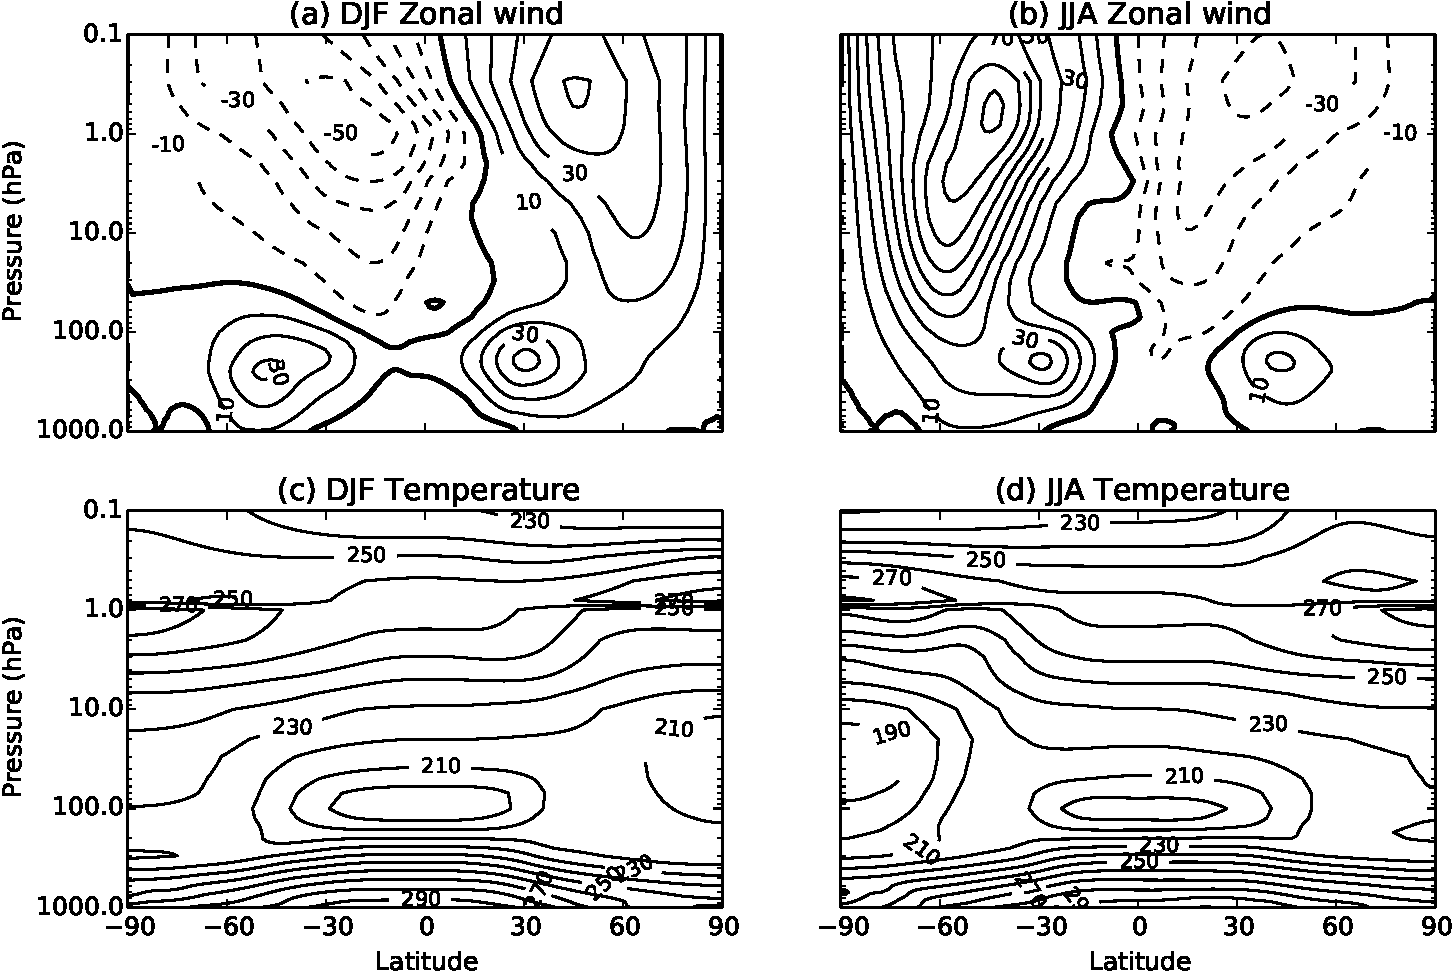
\includegraphics[width=\textwidth]{figures/chapter-intro/zmzw_zmT_clim.pdf}
 \caption[Zonal-mean zonal wind and temperature climatology.]{December-January
   (DJF) (a,c) and July-August (JJA) (b,d) averages of zonal-mean zonal wind
   ($\mathrm{m~s^{-1}}$) (a,b) and temperature (K) (c,d). Dashed contours
   represent negative values. Data is from the ERA-Interim reanalysis
   (1979-2010).}
 \label{fig:zmzw_zmT_clim}
\end{figure}

Figure \ref{fig:zmzw_zmT_clim} shows zonal-mean zonal wind and temperature
averaged over the boreal winter (December-February; DJF) and austral winter
(July-August; JJA) using data from 1979-2010 from the ERA-Interim reanalysis
(details in Section \ref{sec:reanalysis-data}). In both cases the westerly
vortex in the winter hemisphere can be seen along with a local minimum in
temperature at the winter pole in the lower stratosphere. Easterly winds are
present in the summer hemisphere. The maximum strength of the polar vortex
occurs at midlatitudes between 0.1-1~hPa in the mesosphere, and is stronger in
the Southern Hemisphere (SH) with a maximum of $90~\mathrm{ms^{-1}}$ than the
Northern Hemisphere (NH) with a maximum of $50~\mathrm{ms^{-1}}$. The winter
polar stratosphere is also approximately 20~K colder in the SH than the NH.

\begin{figure}
 \centering
 \noindent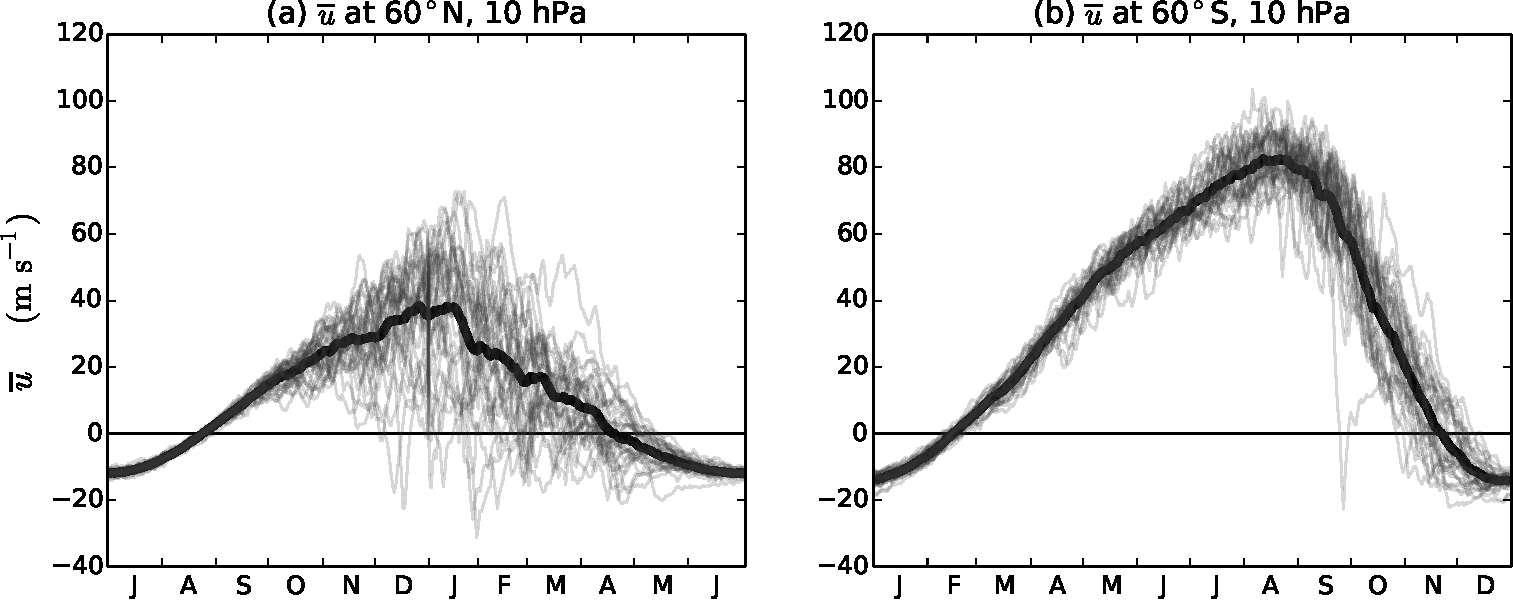
\includegraphics[width=\textwidth]{figures/chapter-intro/zmzw_NH_SH.pdf}
 \caption[Comparison of NH and SH polar vortex seasonal cycle.]{Seasonal cycle
   of NH (a) and SH (b) polar vortex strength, measured by $\overline{u}$ at
   60$^{\circ}$N/S, 10~hPa. The annual mean is shown in a thick black line and
   individual years in thin grey lines. Both time series are centred on their
   respective winters. Data is from the ERA-Interim reanalysis (1979-2010).}
 \label{fig:zmzw_NH_SH}
\end{figure}

The maximum strength of the vortex in the stratosphere occurs at approximately
$60^{\circ}$N/S with little variation through the depth of the
stratosphere. Figure \ref{fig:zmzw_NH_SH} shows the annual cycle and variability
of zonal-mean zonal wind at 10~hPa $60^{\circ}$N and $60^{\circ}$S. As well as
being weaker on average than the SH, the winter NH stratospheric polar vortex
can also be seen to be significantly more variable than the SH. There are a
number of years in the NH for which $\overline{u}$ becomes negative during the
winter, but only one such year in the SH (these events are discussed further in
Section \ref{sec:strat-sudd-warm}). A further clear feature of both NH and SH is
that variability during the summer is much less than that during winter. Also,
the transition to summer easterlies (known as the final warming) occurs
relatively earlier in the seasonal cycle in the NH than the SH. All these
observations are due almost entirely to the influence of wave phenomena in the
stratosphere, as described in the next section.


\subsection{Waves in the stratosphere}
\label{sec:plan-waves-strat}

\subsubsection{Planetary waves}
\label{sec:planetary-waves}

Large-scale Rossby or planetary waves\footnote{Here, as is common in the
  stratospheric literature, ``wave'' is taken to mean any deviation from the
  zonal-mean state.} play a vital
role in the dynamics of the extratropical stratosphere. They mostly enter the
stratosphere from the troposphere, where they are forced, for example, by air
flow around topography, latent heat release, or nonlinear evolution of
tropospheric eddies \citep{Scinocca1998}. These large-scale waves approximately
satisfy the quasi-geostrophic (QG) approximation of hydrostatically balanced
incompressible flow with low Rossby number, $\mathrm{Ro} = U/f_oL \ll 1$, where
$U$ and $L$ are characteristic velocity and length scales respectively
\citep{Andrews1987}. Under this approximation and in the absence of friction,
the following relation, known as the \emph{quasi-geostrophic potential vorticity
  equation}, holds:
\begin{equation}
D_gq_g = f_0\rho_0 \frac{\partial}{\partial z}
\frac{\rho_0Q}{\partial\theta_{0}/\partial z} \, . 
\label{eq:qgpv}
\end{equation}
Where
\begin{equation}
D_g \equiv \frac{\partial}{\partial t} + u_g\frac{\partial}{\partial x} +
v_g\frac{\partial}{\partial y} \, , 
\end{equation}
and 
\begin{equation}
  q_g = f_0 + \beta y - \frac{\partial v_g}{\partial x} + \frac{\partial u_g}{\partial
    y} + \rho_o^{-1}\frac{\partial}{\partial
    z}\left(\rho_of_0\frac{\theta_e}{\partial\theta_{0}/\partial z}\right) \, , 
\end{equation}
is the quasi-geostrophic potential vorticity. Here, $v_g$ is the geostrophic
meridional velocity, $v_g = f^{-1}\partial Z/\partial x$, $Q$ is the diabatic
heating rate, $\rho_0$ is a reference density and $\theta_0$ is a reference
potential temperature, $\theta_0 = T_s(p_s/p)^\kappa$, where
$p_s=1000~\mathrm{hPa}$, and $\kappa = R/c_p \approx 2/7$, where $c_p$ is the
specific heat capacity of air at constant pressure. $\theta_e$ represents the
departure from $\theta_0$, and is assumed to be small in the sense that
$|\partial\theta_e/\partial z| \ll |\partial\theta_0/\partial z|$. An important
consequence of Equation \ref{eq:qgpv} is that $q_g$ is conserved following the
geostrophic wind for adiabatic flow ($Q=0$), and therefore acts as a tracer.
\footnote{Throughout most of this thesis, Ertel's potential vorticity, $q$,
  is used. This is defined by
\begin{equation*}
  q = \frac{1}{\rho}\zeta\cdot\nabla\theta \, , 
\end{equation*}
where
$\zeta$ is the absolute vorticity. \citet{Charney1962} showed that when the
quasi-geostrophic approximation is valid
\begin{equation*}
\left(\frac{\partial q}{\partial s}\right)_{\theta=\mathrm{const.}} \approx
\frac{1}{\rho_0}\frac{\partial \theta_0}{\partial z}\left(\frac{\partial
    q_g}{\partial s}\right)_{z=\mathrm{const.}} \, ,
\end{equation*}
where $s = t$, $x$ or $y$. Hence, a similar conservation law as for
$q_g$ applies to $q$, which is conserved on isentropic (e.g., constant
$\theta$) surfaces.  }

In the case of approximately zonal flow $[\overline{u}(y,z),0,0]$, Equation
\ref{eq:qgpv} can be linearised to give
\begin{equation}
\left(\frac{\partial}{\partial t} + \overline{u}\frac{\partial}{\partial
    x}\right)q_g' + v'\frac{\partial\overline{q_g}}{\partial y} = f_0\rho_0 \frac{\partial}{\partial z}
\frac{\rho_0Q'}{\partial\theta_{0}/\partial z} \, ,
\label{eq:linear_qgpv} 
\end{equation}
where primes represent deviations from the zonal mean (e.g., $q_g =
\overline{q_g} + q_g'$). It can be shown that Equation \ref{eq:linear_qgpv}
supports wave-like solutions, with vertical propagation dependent upon the
condition:
\begin{equation}
0 < \overline{u}-c < \overline{u}_c \equiv \beta(k^2+l^2+\epsilon/4H^2)^{-1} \,,
\end{equation}
which is known as the \emph{Charney-Drazin criterion} after
\citet{Charney1961}. Here, $c$ is the wave's zonal phase speed, $k$ and $l$ are
the zonal and meridional wavenumbers respectively, and $\epsilon = f_0^2/N^2$,
where $N^2 = H^{-1}Re^{-\kappa z/H}\partial\theta_0/\partial z$ is the static
stability. In the case of waves whose phase is stationary with respect to the
ground ($c=0$), this simplifies to
\begin{equation}
0 < \overline{u} < \overline{u}_c\, . 
\label{eq:charney-drazin}
\end{equation}
It is therefore apparent that in order for planetary waves to propagate
vertically (such as from the troposphere to the stratosphere), a westerly flow
must be present that is not too strong. Additionally, this maximum speed is
dependent on wavenumber, such that a lower wavenumber can propagate in a
stronger westerly flow. While the assumptions here are not representative of the
real atmosphere (such as purely zonal flow, and small deviations from the zonal
mean), this criterion does capture the most important features of the relation
between zonal assymmetries and the zonal flow, and similar relations can be
found for more complex background states \citep{Andrews1987}.

An important consequence of the Charney-Drazin criterion for stratospheric flow
is that the strength of the stratospheric polar vortices shown in Figures
\ref{fig:zmzw_zmT_clim} and \ref{fig:zmzw_NH_SH} is often sufficient to exclude
all but the lowest wavenumbers (typically zonal wavenumbers 1--3; hereafter
referred to as `wave-$n$') from propagating upwards from the troposphere. Hence
the length-scale of typical stratospheric zonal asymmetries is much larger than
that of the troposphere.

\bigskip When planetary waves reach a \emph{critical surface}, where propagation
is prohibited (for instance, a region where $\overline{u} = c$), the above
linear analysis breaks down. In this scenario waves can ``break'', imparting
momentum onto the zonal flow. There is therefore a two-way interaction between
the zonal flow and planetary waves; a phenomenon known as \emph{wave-mean flow
  interaction}. Wave breaking was studied in an idealised two-dimensional model
by \citet{Stewartson1978} and \citet{Warn1978}. They found momentum to be
absorbed in a narrow \emph{critical layer} close to the critical surface, with
potential vorticity (PV) contours being irreversibly stretched and mixed in
increasingly fine scales; a process known as a `potential enstrophy cascade'
\citep[e.g.,][]{Rhines1979}. They also showed that the critical layer is
initially absorbing, but becomes a reflecting surface after some time. Time
varying results from a version of the Stewartson-Warn-Warn model from
\citet{Andrews1987} are shown in Figure \ref{fig:cats_eyes}. Similar wave
breaking behaviour was first observed in the real stratosphere by
\citet{McIntyre1983} using isentropic maps of Ertel's potential vorticity,
including the irreversible deformation of PV contours of the kind shown in
Figure \ref{fig:cats_eyes}.

\begin{figure}
 \centering
 \noindent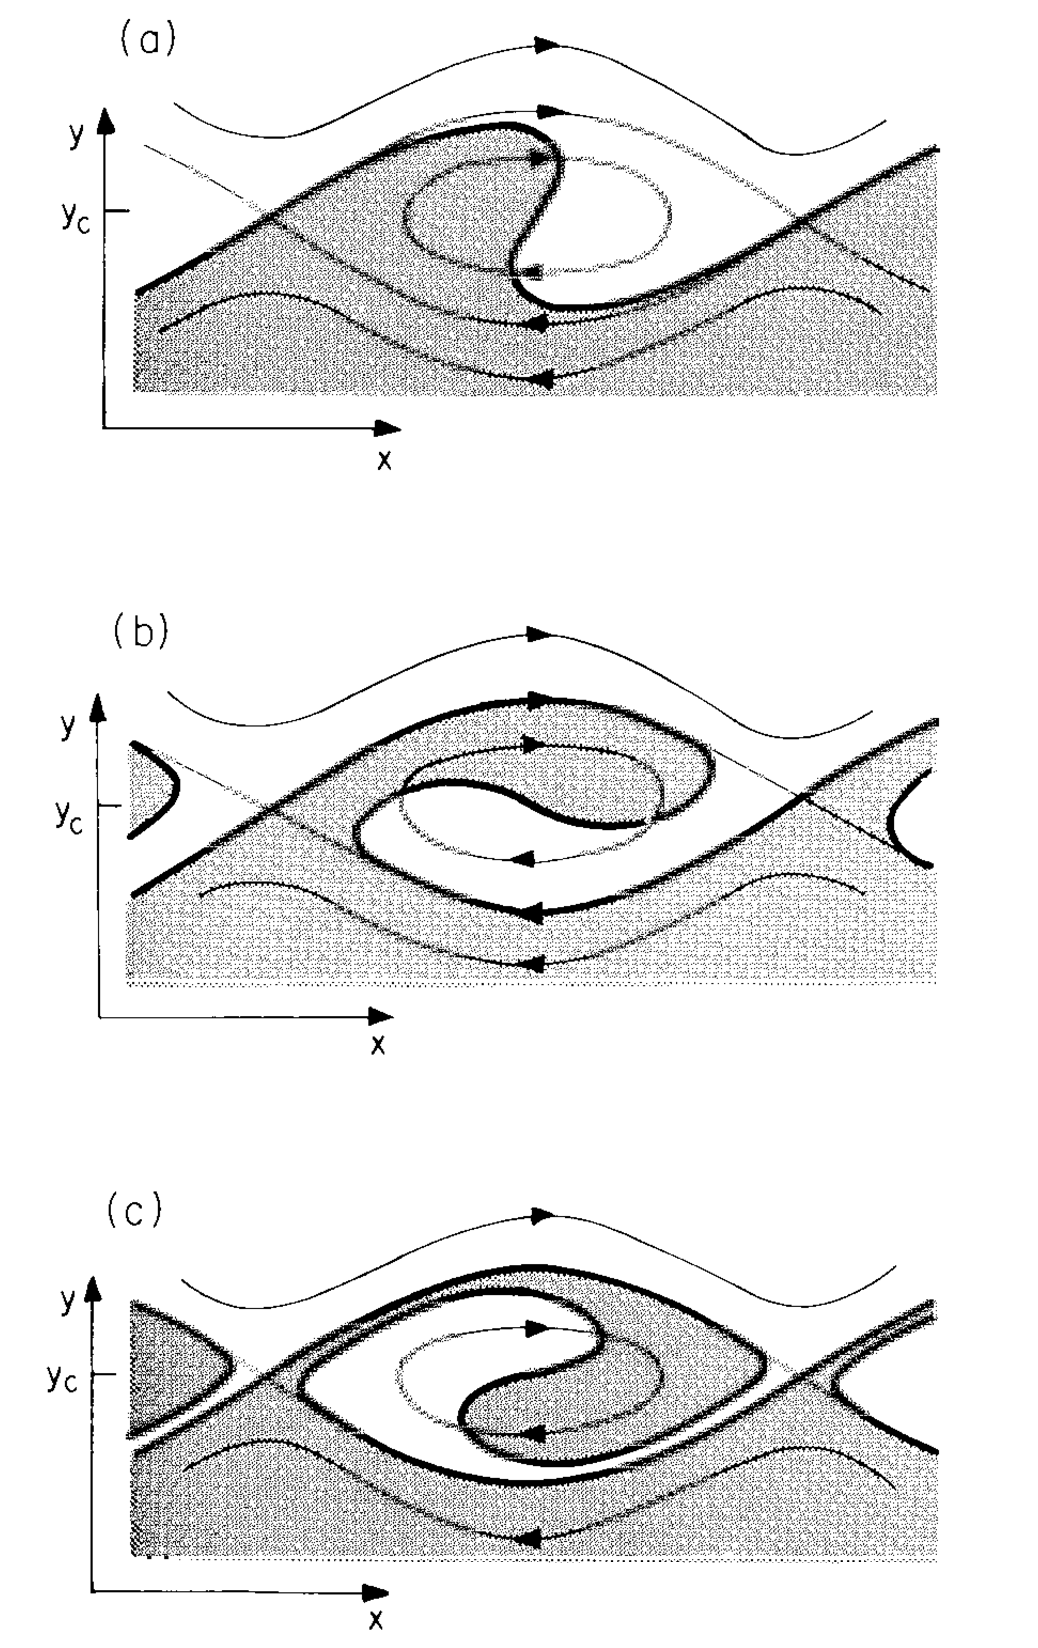
\includegraphics[width=0.6\textwidth]{figures/chapter-intro/breaking_wave_AHL.pdf}
 \caption[Results from a Stewartson-Warn-Warn model of wave
 breaking.]{Stewartson-Warn-Warn time-dependent analytical solution of a Rossby
   wave nonlinear critical layer (time advancing in even steps from
   (a)-(b)-(c)). The flow is periodic in $x$ and the $y$ scale is greatly
   exaggerated and the initial critical line was at $y=y_c$. The thin lines
   indicate streamlines and lens shaped regions of closed streamlines are known
   as ``Kelvin's cats' eyes''. The thick line shows the position of the absolute
   vorticity contour $\zeta=\zeta_c$, that initially lay along $y=y_c$ (in this
   barotropic model, the quasi-geostrophic potential vorticity, $q_g$, reduces
   to $\zeta$). Hence, $\zeta<\zeta_c$ in the stippled region and
   $\zeta>\zeta_c$ in the unstippled region. In (a) it can be seen that $v>0$
   for most of the stippled region, indicating partial absorption, whereas in
   (b) and (c) $v\leq0$ in the stippled region indicating reflection. Figure
   from \citet{Andrews1987}.}
 \label{fig:cats_eyes}
\end{figure}

A further effect of wave breaking is the induction of a \emph{residual
  circulation}, $[0, \overline{v}^*, \overline{w}^*]$, where $\overline{v}^*$ and
$\overline{w}^*$ are the transformed Eulerian-mean (TEM) meridional and vertical
velocities given in spherical coordinates by
\begin{equation}
  \overline{v}^* = \overline{v} - \frac{1}{\rho_0}\frac{\partial}{\partial z}
  \left(\frac{\rho_o\overline{v'\theta'}}{\partial\overline{\theta}/{\partial z}}\right) \, , 
\end{equation}
\begin{equation}
\overline{w}^* = \overline{w} + \frac{1}{a\cos\phi}\frac{\partial}{\partial\phi}
\left(\frac{\cos\phi\overline{v'\theta'}}{\partial\overline{\theta}/{\partial
      z}}\right) \, ,
\end{equation}
which approximates the Lagrangian-mean circulation under time-averaged
conditions \citep{Andrews1976,Dunkerton1978,Holton1990}. Under the TEM
formalism, the zonal momentum equation becomes
\begin{equation}
\frac{\partial\overline{u}}{\partial t} +
\overline{v}^*\left(\frac{1}{a\cos\phi}\frac{\partial}{\partial\phi}(\overline{u}\cos{\phi})
  - f \right) + \overline{w}^*\frac{\partial\overline{u}}{\partial z} =
\frac{\mathbf{\nabla \cdot F}}{\rho_oa\cos\phi} + \overline{X} \equiv \overline{\mathcal{F}}
\label{eq:zonal_momentum}
\end{equation}
where $\overline{X}$ represents frictional terms and $\mathbf{F}=[0,F^\phi,F^z]$
is the Eliassen-Palm (EP) flux with components
\begin{equation}
F^\phi = \rho_0a\cos\phi\left(\frac{\partial\overline{u}}{\partial
    z}\frac{\overline{v'\theta'}}{\partial\overline{\theta}/\partial z} -
  \overline{v'u'}\right) \, ,
\end{equation}
\begin{equation}
F^z =
\rho_0a\cos\phi\left(\left[f-\frac{1}{a\cos\phi}\frac{\partial}{\partial\phi}(\overline{u}\cos\phi)\right]\frac{\overline{v'\theta'}}{\partial\overline{\theta}/\partial
      z} - \overline{w'u'}\right) \, .
\end{equation}
$\mathbf{F}$ can be interpreted as the flux of wave activity
\citep{Andrews1987}, and therefore $\mathbf{\nabla\cdot F}<0$ (convergence)
represents a dissipation of wave activity, as is the case in wave breaking. It
can be seen that for a steady zonal flow ($\partial\overline{u}/\partial t = 0$)
in the absence of wave driving ($\mathbf{\nabla\cdot F} = 0$) or friction
($\overline{X} = 0$), a solution of Equation \ref{eq:zonal_momentum} is
$\overline{v}^*=0, \overline{w}^*=0$.  However, in the presence of these forcing
terms, a non-zero residual circulation will be induced. Climatologically, this
circulation consists of wave-driven poleward and downward motion in the
extratropics which is balanced by upwelling in the tropics; a pattern which
forms a significant part of the Brewer-Dobson circulation\footnote{Strictly, the
  Brewer-Dobson circulation represents the meridional transport of tracers, and
  so also involves two-way mixing (i.e. transport without net transfer of mass)
  \citep{Hall1994}.}. The downward motion near the poles can be easily seen from
Equation \ref{eq:zonal_momentum} in the steady case; since $\overline{v}^*$ must
become small near the poles (by conservation of mass), and
$\partial\overline{u}/\partial z > 0$ in the polar vortex, if
$\mathbf{\nabla\cdot F} < 0$, then $\overline{w}^*<0$. It is observed that this
circulation is strongest in the winter hemisphere due to the fact that more
planetary waves can propagate and break in the winter westerly flow than the
summer easterly flow (due to the Charney-Drazin criterion). Furthermore, during
periods of enhanced wave breaking the residual circulation accelerates and there
is more descent and adiabatic heating at high latitudes. This is important in
the physical understanding of sudden stratospheric warming events, described in
Section \ref{sec:strat-sudd-warm}.


\subsubsection{Gravity waves}

Gravity waves are another type of atmospheric wave important in the dynamics of
the polar stratosphere. These waves owe their existence to buoyancy restoring
forces and can be generated by a number of processes such as air flow over
topography (orographic gravity waves), convection or frontogenesis
(non-orographic gravity waves). As with planetary waves, the differences in the
land masses of the two hemispheres leads to orographic gravity wave activity
being much greater in the NH. These waves make a net easterly contribution to
the winter zonal flow \citep[e.g.,][]{Seviour2012}, and so act to enhance the
residual circulation. Their typical length scales are much shorter than can be
resolved in general circulation models or reanalyses, and so they are usually
parametrised, appearing as the term $\overline{X}$ in the zonal momentum
equation (Equation \ref{eq:zonal_momentum}).
\begin{center}
\line(1,0){250}
\end{center}

Together, the Charney-Drazin criterion and the effects of planetary and
gravity wave driving on the zonal flow can expain almost all hemispheric
differences seen in Figures \ref{fig:zmzw_zmT_clim} and \ref{fig:zmzw_NH_SH}:
Greater topography results in more planetary and gravity wave generation in the
NH, both of which cause a net deceleration of the westerly polar vortex, thereby
causing the NH vortex to be weaker than the SH. This also explains why the NH
vortex is warmer than the SH, as the greater NH wave activity induces a stronger
residual circulation with enhanced descent and adiabatic warming at high
latitudes. Additionally, the strength of the SH vortex is such that it prohibits
the vertical propagation of planetary waves from the troposphere throughout much
of the winter, meaning that the SH vortex is less variable than the NH. Both
hemispheres show very little variability in the summer easterly flow because
planetary wave propagation is prohibited in this regime.


\subsection{Sudden stratospheric warmings}
\label{sec:strat-sudd-warm}
%footnote on name
First observed by \citet{Scherhag1952} in radiosonde measurements over Berlin,
the extreme events visible in Figure \ref{fig:zmzw_NH_SH} whereby the winter
circulation temporarily becomes easterly\footnote{For a discussion of more
  precise definitions of SSWs, see Section \ref{sec:moments-introduction}.} are
known as sudden stratospheric warmings\footnote{Following \citet{Butler2014a} it
  is suggested that the term ``sudden stratospheric warming'' is preferable to
  the common alternative ``stratospheric sudden warming''. This is because there
  are other varieties of stratospheric warming (such as final warmings or
  Canadian warmings), but not other varieties of atmospheric sudden warming.}
(SSWs). These events occur approximately 5-7 times per decade in the NH, but
only one such event has been observed in the almost 60 year observational record
in the SH (in 2002). They are called ``warmings'' because associated with the
circulation reversal is a dramatic increase in temperature; as much as 50~K in
the space of a few days in the mid-stratosphere.\footnote{A recent study
  \citep{Neef2014} has even suggested that SSWs have a sufficiently strong
  influence on the Earth's angular momentum that they have a detectable
  influence on the length of the day.}

Initially these events were thought to result from either solar storms or
baroclinic instability of the stratospheric polar vortex. However,
\citet{Matsuno1970, Matsuno1971} proposed a model of SSWs which relies on the
influence of tropospherically forced planetary waves. This model (or
modifications thereof) remains the most widely accepted dynamical view of SSWs
at present. The mechanism proceeds as follows:
\begin{enumerate}[i.]
\item A packet of enhanced planetary wave activity enters the stratosphere where
  it reaches a critical surface and breaks. This decelerates the zonal flow over
  a broader critical layer, and if strong enough causes it to reverse.
\item Hence a new critical surface is formed at a lower level (where
  $\overline{u}=0$), and wave breaking occurs at this level. The process
  continues as the critical layer descends to the lower stratosphere.
\item At the same time, wave breaking induces an enhanced residual circulation
  with greater descent and adiabatic warming at high latitudes. If strong
  enough, this can act to reverse the meridional temperature gradient, further
  enhancing the easterly flow by thermal wind balance. 
\item When the critical surface is close to the tropopause, planetary wave
  activity is essentially prohibited from entering the polar
  stratosphere. Radiative cooling to space then acts to cool the polar
  stratosphere and the vortex reforms over a period of approximately 2-4 weeks.
\end{enumerate}

This mechanism considers the effect of planetary waves on the zonal-mean
flow. However, it has been observed that SSWs generally occur as either a split
or displacement of the vortex, mostly depending (though not exclusively; see
Section \ref{sec:moments-introduction}, \citep{Waugh1997}) on whether wave-2 or
wave-1 activity is dominant. An example of each of these events is shown in
Figure \ref{fig:charlton_polvani_ssw}. \citet{Charlton2007} and
\citet{Matthewman2009} studied the dynamics of these two types of events in
reanalysis data and noted some differences. Most significantly, split vortex
events were observed to occur near-barotropically, with two smaller vortices
centred over Canada and Siberia throughout the depth of the stratosphere. On the
other hand, displaced vortex events were observed to be more baroclinic,
starting first in the upper stratosphere with a vortex centred over Canada, the
centre of which rotates westward with height and is centred over Siberia in the
lower stratosphere.


\begin{figure}
 \centering
 \noindent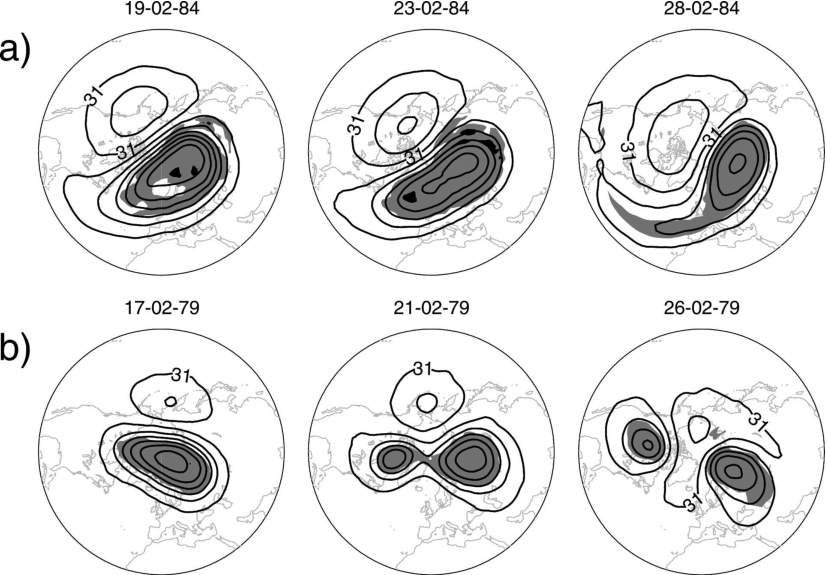
\includegraphics[width=\textwidth]{figures/chapter-intro/charlton_polvani_SSW.pdf}
 \caption[Examples of a split and displaced vortex event from
 \citet{Charlton2007}]{Polar stereographic plot of geopotential height
   (contours) on the 10~hPa pressure surface. Contour interval is 0.4~km, and
   shading shows potential vorticity greater than
   $4.0 \times 10^{-6} \mathrm{K~kg^{-1}~m^2~s^{-1}}$. (a) A vortex displacement
   type warming that occurred in February 1984. (b) A vortex splitting type
   warming that occurred in February 1979. Figure from \citet{Charlton2007}.}
 \label{fig:charlton_polvani_ssw}
\end{figure}

This different behaviour of split and displaced vortex events is not accounted
for by the \citet{Matsuno1970, Matsuno1971} model above, and so may suggest that
other mechanisms are important in the generation of SSWs. For instance,
\citet{ONeill1988} and \citet{Scott2006} have suggested that SSWs can be
generated by a cyclone-anticyclone interaction between the Aleutian high and the
polar vortex. These studies showed that a smaller anticyclone can act to
significantly distort the polar vortex, although such interactions are greatest
for circulation ratios higher than are typically found in the polar
stratosphere. Other studies have suggested that SSWs can arise through the
resonant excitation of normal modes of the stratosphere by planetary waves
\citep{Tung1979}. Significantly, \citet{Plumb1981} found that the planetary wave
forcing need not be at exactly the resonant frequency of the mode (an occurrence
which is probably unlikely), but that the two can be brought to resonance by a
process known as nonlinear ``self-tuning''. \citet{Smith1989} found behaviour
suggestive of this process in simulations of a SSW. More recently,
\citet{Esler2005} and \citet{Esler2006} suggested that a relevant mode in the
case of split vortex events is the barotropic mode of the atmosphere, which may
explain the more barotropic nature of split vortex events.

Further weight is given to these mechanisms which do not rely on strong
transient tropospheric forcing by the occurrence of the 2002 SH SSW, since this
forcing is much weaker in the SH (several studies of the dynamics of this event
can be found in the March 2005 special issue of \emph{Journal of Atmospheric
  Sciences}). Indeed, \citet{Esler2006} provided evidence that this event may
have been influenced by resonant excitation of the barotropic mode.

%It should also be noted that other studies have suggested that SSWs can occur
%even in the case of no tropospheric stationary forcing \citep{Kushner2005}.

Several studies have also discussed the role of the polar vortex being in a
favourable (or `preconditioned') state prior to SSWs
\citep[e.g.,][]{McIntyre1982}. In a simple dynamical model, \citet{Scott2004}
demonstrated that planetary wave breaking is enhanced by the presence of steep
PV gradients at the vortex edge, which are likely to be present in an
anomalously strong vortex. Indeed, \citet{Limpasuvan2004} found evidence for an
anomalously strong vortex 30-40 days prior to SSWs, while \citet{Charlton2007}
found this effect to be stronger prior to split vortex events than displaced
vortex events. 

Overall, while significant advances in understanding the dynamics of SSWs have
been made, several uncertainties remain. Tropospherically-driven wave activity
is certainly an important factor but the roles (if any) of cyclone-anticyclone
interactions or resonance are less certain. Moreover, it is not clear whether
different mechanisms may be more or less important in driving split and
displaced vortex events.


\section{Polar stratospheric ozone depletion}
\label{sec:polar-strat-ozone}

The Antarctic ozone hole is a large region of severely depleted ozone
concentrations in the lower-mid stratosphere which occurs during the austral
spring. During its formation ozone is often be completely destroyed at some
altitudes. A similar, but much smaller depletion is observed in the NH
\citep[e.g.,][]{Manney1997}. Following its discovery by \citet{Farman1985}, a
chemical and dynamical theory of the ozone hole was rapidly developed which
largely attributes this rapid ozone depletion to the presence of anthropogenic
chlorofluorocarbon (CFC) compounds \citep{McElroy1986,Solomon1986}. This theory
is summarised as follows:
\begin{enumerate}[i.]
\item The strong zonal winds of the stratospheric polar vortex act to confine
  air over the polar regions, with little mixing with midlatitudes
  \citep{Schoeberl1991}. This results in a region of very cold temperatures
  which allow the formation of polar stratospheric clouds (PSCs; these require
  temperatures below approximately 195~K to form \citep{Newman2010}).
\item Heterogeneous chemical reactions can take place on the surface of PSCs which
  act to convert `reservoir' chlorine species such as \ce{ClONO2} and \ce{HCl}
  into forms that can accelerate ozone depletion, for instance
  \citep{Solomon1986}:
  \begin{equation*}
    \ce{ClONO2 + HCl ->[\ce{PSC}] Cl2 + HNO3}
  \end{equation*}
\item As sunlight returns to the vortex region in spring, \ce{Cl2} is rapidly
  photolysed and reacts with oxygen to form \ce{ClO}. This can then
  catalytically destroy ozone through a reaction sequence such as the following
  suggested by \citet{Molina1987}:
  \begin{align*}
    \cee{ClO + ClO &->[\ce{M}] ClOOCl \\
         ClOOCl + $h\nu$ &-> ClOO + Cl \\
         ClOO &->[\ce{M}] Cl + O2 \\
         2(Cl + O3 &-> ClO + O2) \\
         $\mathrm{Net:~}$ 2O3 &-> 3O2} 
  \end{align*}
  where $\nu$ is the frequency of light,
  $h$ is Planck's constant, and M a third body (necessary for conservation of
  momentum). Several other reaction sequences are also possible, for instance
  involving bromine species.

\item A further effect of PSCs is that their particles fall out of the
  stratosphere and thereby remove nitrogen compounds
  (\ce{NO$_x$}) from the polar lower stratosphere \citep{Toon1986}.
  \ce{NO$_x$} compounds are important because they can react with with \ce{ClO}
  to form reservior compounds. For instance the reaction
  \begin{equation*}
    \ce{ClO + NO2 ->[\ce{M}] ClONO2}
  \end{equation*}
  removes \ce{ClO} from the ozone-depleting sequence above. Hence a reduction of
  \ce{NO$_x$} due to PSCs leads to an increase in ozone depletion.

\item After some time, radiative heating of the stratosphere is sufficient to
  prevent the formation on PSCs, so ozone depletion halts. This heating is
  further accelerated by the increased wave breaking in the polar stratosphere
  which can take place as the vortex weakens (due to the Charney-Drazin
  criterion) and thereby induce an enhanced residual circulation. Following the
  final breakdown of the vortex and transition to summer easterlies (final
  warming), the ozone-depleted air is mixed to lower latitudes.
\end{enumerate}

\begin{figure}
 \centering
 \noindent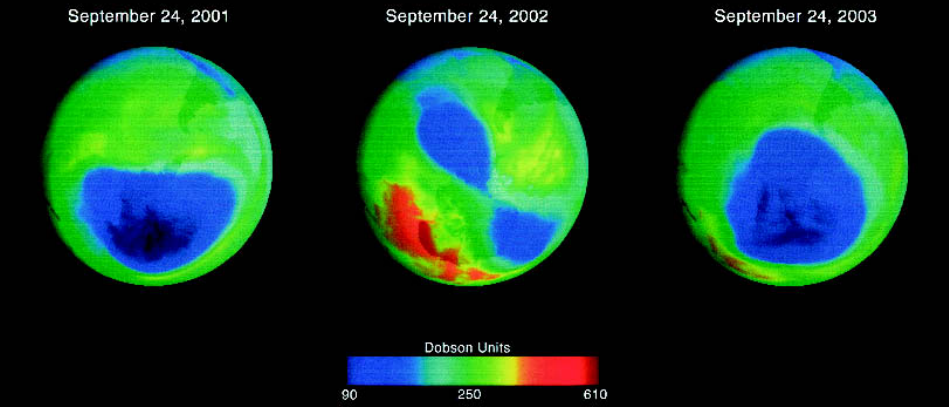
\includegraphics[width=\textwidth]{figures/chapter-intro/2002_SSW.png}
 \caption[]{Comparison of the (middle) first split ozone hole on record (2002)
   and (left) the Antarctic ozone hole at the same time one year earlier (2001)
   and (right) one year later (2003). The hole is dark blue and magenta. In
   2001, the ozone layer thinning over Antarctica reached
   $26.5 \times 10^6~\mathrm{km^2}$ , larger than the size of the entire North
   American continent. Due to higher Antarctic winter temperatures, the 2002
   ``hole'' seems to be about 40\% smaller. In 2003, Antarctic winter
   temperatures returned to normal and the ozone hole returned to its usual
   state. Figure from \citet{Shepherd2005}.}
 \label{fig:2002_SSW}
\end{figure}

Importantly, the stratospheric dynamics described in Section
\ref{sec:dynam-polar-strat}, play an important role in ozone depletion. As
discussed in Section \ref{sec:planetary-waves}, wave breaking in the
stratosphere acts to drive a residual circulation, with descent and adiabatic
warming over the pole. Enhanced descent and warming over the pole acts to
inhibit the formation of PSCs which are necessary for the above heterogeneous
chemical reactions which cause ozone depletion. A stronger meridional
circulation also acts to transport more tropical ozone-rich air to the polar
regions, further acting to increase ozone concentrations. Another mechanism in
which wave breaking acts to inhibit ozone depletion is by actively stripping
away filaments of ozone-depleted air from the polar vortex \citep{Waugh1994}. It
is this greater wave activity in the NH then that explains why the extent of
ozone depletion is much less in the NH than the SH.

%Moreover, it has been demonstrated that interannual variability in wave driving
%can account for most of the interannual variability of ozone depletion through
%this mechanism \citep{Salby2012}.

In the extreme event of SSWs, the ozone hole can be severely disrupted. This can
be seen in Figure \ref{fig:2002_SSW}, where a clear split of the ozone hole is
visible during the 2002 SH SSW, which contrasts with the more zonally symmetric
distributions seen at the same times in 2001 and 2003. The magnitude of the 2002
ozone hole can also be seen to be reduced; a result of an enhanced residual
circulation causing warmer stratospheric temperatures. The importance of this
link between dynamics and chemistry for predicting interannual variability in
ozone depletion is discussed further in Sections \ref{sec:ozone-depletion} and
\ref{sec:seas-discussion}.

\section{Annular modes}
\label{sec:annular-modes}
Before discussing the influence of the stratosphere on the troposphere, it is
necessary to introduce the concept of the annular modes which are often analysed
in studies on this topic (as well as in this thesis). The northern and southern
annular modes (NAM and SAM) are the leading modes of large-scale variability in
the two hemispheres
\citep{Baldwin1999,Thompson2000a,Thompson2000,Limpasuvan1999,Limpasuvan2000}. They
are commonly defined to be the leading empirical orthogonal function
(EOF)\footnote{EOFs are the eigenvectors of the spatially weighted covariance
  matrix of a variable. EOF analysis is also known as principal component
  analysis \citep{Wilks}.} of extratropical monthly-mean geopotential height
calculated at each pressure surface \citep[e.g.,][]{Baldwin1999}, with an index
of the respective principal component or the projection of daily data onto the
EOF pattern. \citet{Baldwin2009} introduced an alternative using zonal-mean
geopotential height, which is therefore less computationally expensive to
calculate. The annular modes at the surface are also often calculated from mean
sea-level pressure \citep[e.g.,][]{Gong1999}, where they may also be referred to
as the Arctic and Antarctic oscillation (although in this thesis, the terms
\emph{surface NAM/SAM} are used).

Figure \ref{fig:annular_modes} shows linear regressions of zonal-mean
geostrophic winds and lower tropospheric geopotential height on the NAM and SAM
indices as defined by \citet{Thompson2000a}. It can be seen that the
near-surface NAM structure is more zonally asymmetric than the SAM, with centres
of action located over the Atlantic and Pacific oceans, and the SAM has a more
clearly `annular' structure. The vertical structure of the NAM and SAM appears
near barotropic, although with a slight poleward tilt with
height.\footnote{\citet{Thompson2014} have recently argued that the barotropic
  and baroclinic aspects of the SAM can be viewed as two independent modes of
  variability.} The magnitude of the zonal wind signature also increases with
height, reaching a maximum in the upper troposphere/lower stratosphere in the
SH, and the mid-stratosphere in the NH.

Despite this near-barotropic appearance, annular mode variability has quite
different physical interpretations in the troposphere and
stratosphere. Stratospheric variability is associated with approximately zonally
symmetric strengthening and weakening of the stratospheric polar vortex, while
tropospheric variability is more closely associated with meridional shifts in
the eddy-driven jets \citep{Limpasuvan1999}. Furthermore, stratospheric annular
mode variability is largely confined to winter, while tropospheric variability
has a much less pronounced seasonal cycle.

It can be seen from Figure \ref{fig:annular_modes}(d) that the Atlantic centre
of action of the NAM resembles the familiar North Atlantic Oscillation (NAO)
pattern. Indeed, the surface NAM and NAO have been observed to be highly
correlated \citep{Ambaum2001}. This has led to some debate as to whether the NAM
represents a physical mode of variability of which the NAO is just a regional
manifestation, or whether the NAM is simply a statistical artifact of more
regional variability. This point is addressed in Section
\ref{sec:meas-strat-trop}.

% Mention recent thompson 2014 and baroclinic mode etc. 
\begin{figure}
 \centering
 \noindent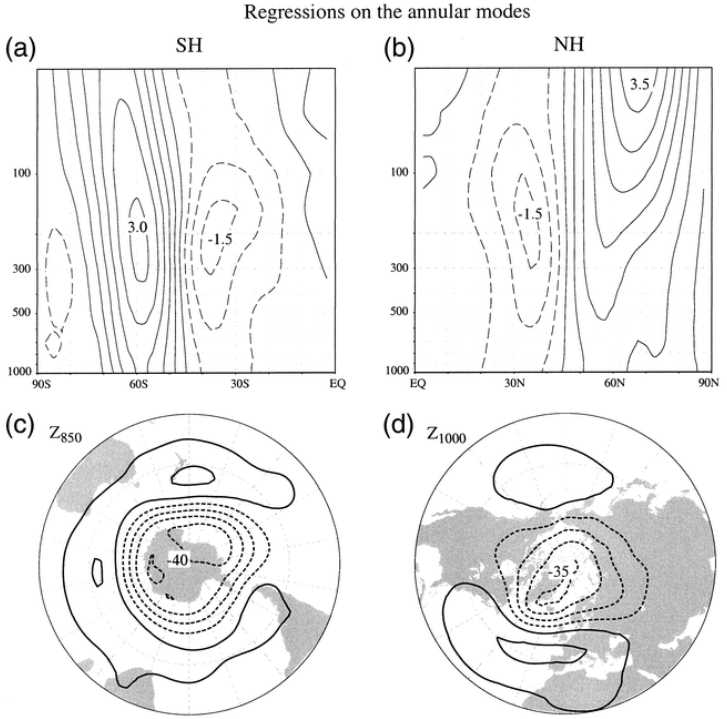
\includegraphics[width=0.7\textwidth]{figures/chapter-intro/annular_modes_TW2.png}
 \caption[Annular mode patterns from \citet{Thompson2000a}]{(top) Zonal-mean
   geostrophic wind and (bottom) lower-tropospheric geopotential height
   regressed on the standardised indices of the annular modes (the AO and its SH
   counterpart) based upon monthly data, Jan 1958--Dec 1997. Left panels are for
   the SH, right panels are for the NH. Units are $\mathrm{m~s^{-1}}$ (top) and
   m per std dev of the respective index time series (bottom). Contour intervals
   are 10~m ($-15,~-5,~5,~\dots$) for geopotential height and
   $\mathrm{0.5~m~s^{-1}}$ ($-0.75,~-0.25,~0.25$) for zonal wind. Figure from
   \citet{Thompson2000a}.}
 \label{fig:annular_modes}
\end{figure}


\section{Stratosphere-troposphere coupling}
\label{sec:strat-trop-coupl}

So far this chapter has dealt with the dynamics of the stratosphere as
responding passively to tropospheric forcing from below. Indeed, this was the
dominant view until the last two decades \citep[e.g.,][]{Andrews1987}. However
observational evidence supported by modelling studies and some theoretical
arguments, have now provided evidence that variability of the polar stratosphere
can significantly influence tropospheric weather and climate. This section
reviews this evidence.



\subsection{Observational evidence}
\label{sec:observ-evid}

The accumulation of observational evidence for a two-way dynamical link between
the polar stratosphere and the troposphere began in the early
1990s. \citet{Kodera1990} found that the strength of the NH upper stratospheric
polar vortex during December was correlated with the strength of the
tropospheric eddy-driven jet in February. However, they did not investigate the
mechanism for this relation, and suggested it may be radiative. Further evidence
was provided by \citet{Nigam1990} who found barotropic and baroclinic modes of
the zonal-mean zonal wind which vary coherently in the troposphere and
stratosphere. This analysis was extended by \citet{Baldwin1994} who found
significant correlations between stratospheric and tropospheric EOFs of daily NH
geopotential height (patterns which would now be referred to as annular
modes). However, they found that the strongest correlations occurred with the
troposphere leading, and while suggesting that the stratosphere may exert some
influence on the troposphere, they concluded that the direction of causality was
mostly upwards.

These studies were followed by several others which looked at the co-variability
of the stratospheric and tropospheric annular modes, and demonstrated links
between the strength of the polar vortex and surface temperature and sea level
pressure patterns \citep{Perlwitz1995, Thompson1998,Baldwin1999}. However, it
was \citet{Baldwin2001a} who first demonstrated that the
stratosphere-troposphere link is particularly strong following extreme
weakenings or strengthenings of the stratospheric polar vortex. Figure
\ref{fig:baldwin_dunkerton} shows a time series of the NAM during the winter of
1998--1999, which includes two such weak vortex events (in December and
February), characterised by a negative stratospheric NAM (these events are
highly correlated with SSWs). It is apparent that the NAM signal appears to
descend in the case of the latter event (but not the former) and consistent
anomalies remain in the troposphere for approximately one month. This timescale
is much longer than the usual timescales of tropospheric NAM variability
\citep[e.g.,][]{Simpson2011} but is more representative of the time taken for
the stratosphere polar vortex to recover following a SSW.

%\begin{figure}
% \centering
% \noindent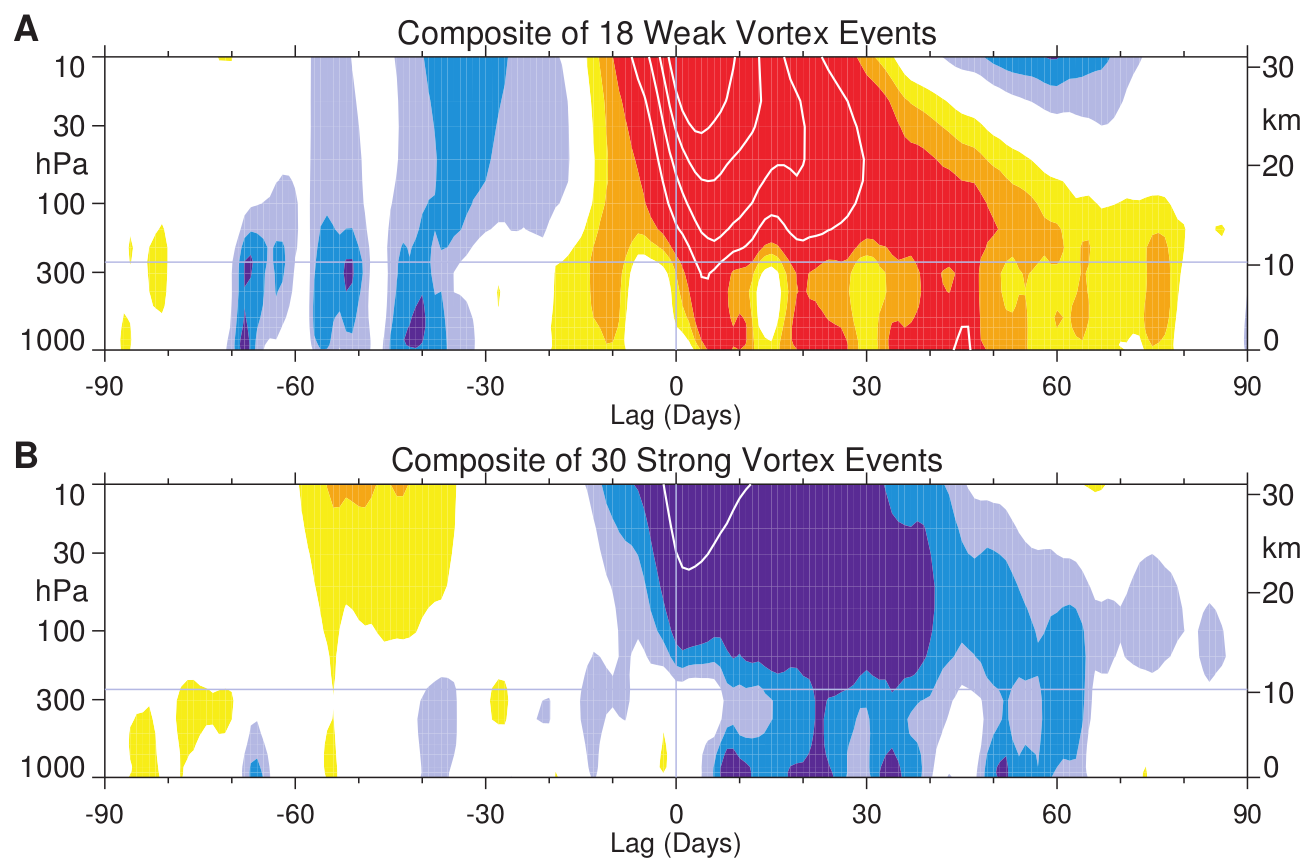
\includegraphics[width=\textwidth]{figures/chapter-intro/Baldwin_Dunkerton.png}
% \caption[NAM composite from \citet{Baldwin2001a}]{Composites of time-height
%   development of the northern annular mode for (A) 18 weak vortex events and
%   (B) 30 strong vortex events. The events are determined by the dates on which
%   the 10-hPa annular mode values cross –3.0 and +1.5, respectively. The indices
%   are nondimensional; the contour interval for the colour shading is 0.25, and
%   0.5 for the white contours. Values between −0.25 and 0.25 are unshaded. The
%   thin horizontal lines indicate the approximate boundary between the
%   troposphere and the stratosphere. Figure from \citet{Baldwin2001a}.}
% \label{fig:baldwin_dunkerton}
%\end{figure}

\begin{figure}
 \centering
 \noindent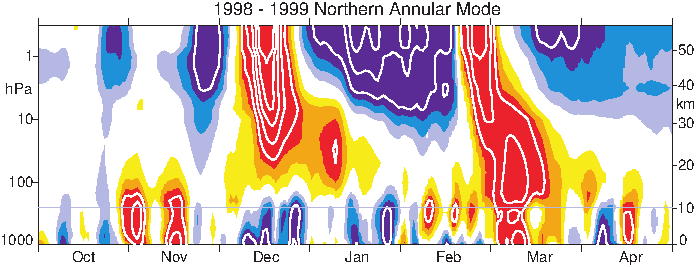
\includegraphics[width=\textwidth]{figures/chapter-intro/Baldwin_Dunkerton_98-99.pdf}
 \caption[NAM time series from \citet{Baldwin2001a}]{Time-height development of
   the northern annular mode during the winter of 1998--1999. The indices have
   daily resolution and are nondimensional. Blue corresponds to positive values
   (strong polar vortex), and red corresponds to negative values (weak polar
   vortex). The contour interval is 0.5, with values between $-0.5$ and 0.5
   unshaded. The thin horizontal line indicates the approximate boundary between
   the troposphere and the stratosphere. Figure from \citet{Baldwin2001a}.}
 \label{fig:baldwin_dunkerton}
\end{figure}

Most observational studies of stratosphere-troposphere coupling have focused on
the NH because of the greater stratospheric variability there. However,
\citet{Thompson2002a} argued that a long-term strengthening of the SH
stratospheric polar vortex resulting from ozone depletion may be causing trends
in the tropospheric SAM through a dynamical link. This was supported by
\citet{Thompson2005}, who performed an analysis similar to \citet{Baldwin2001a},
finding long-lived tropospheric SAM anomalies following strengthenings and
weakenings of the SH stratospheric polar vortex (although these have a much
smaller magnitude to the NH equivalents). They also found a strong tropospheric
SAM signal following the 2002 SH SSW.

More recent studies of tropospheric anomalies following stratospheric events
have focused on more localised extreme weather events in addition to the
annular modes. Several such studies have found associations between weakenings
of the NH stratospheric polar vortex and an increased likelihood of extreme cold
events over North America, northern Europe and eastern Asia \citep{Thompson2002,
  Kolstad2010, Tomassini2012}. These extreme cold events are often linked with
persistent `blocking' weather patterns,\footnote{These are characterised by a
  persistent anticyclonic anomaly that causes a reversal in the
  upper-tropospheric meridional gradient of a quantity such geopotential height
  \citep[e.g.,][]{Tibaldi1990}.}  and a number of studies have investigated the
association between stratospheric variability and blocking. Although
\citet{Taguchi2008} found no statistically significant change in blocking
frequency during periods before or after SSWs, several studies have asserted an
upwards link, with blocking events preceding a weakened polar vortex
\citep{Quiroz1986, Andrews1987, ONeill1994}. More recent studies have further
investigated whether blocking in particular locations precedes split or
displaced vortex events, although these have reached conflicting conclusions
\citep{Martius2009, Woollings2010c, Castanheira2010}. A downwards link between
stratospheric variability and the likelihood of blocking events was suggested by
\citet{Kodera1995}. \citet{Woollings2010c} and \citet{Davini2014} have recently
found more evidence for this link, including stratosphere-leading relationships
between stratospheric variability and high-latitude blocking which may be
associated with the stratospheric impact on the tropospheric NAM. Overall
however, the nature of link between stratospheric variability and blocking
remains uncertain and is a topic of active research.

\begin{figure}
 \centering
 \noindent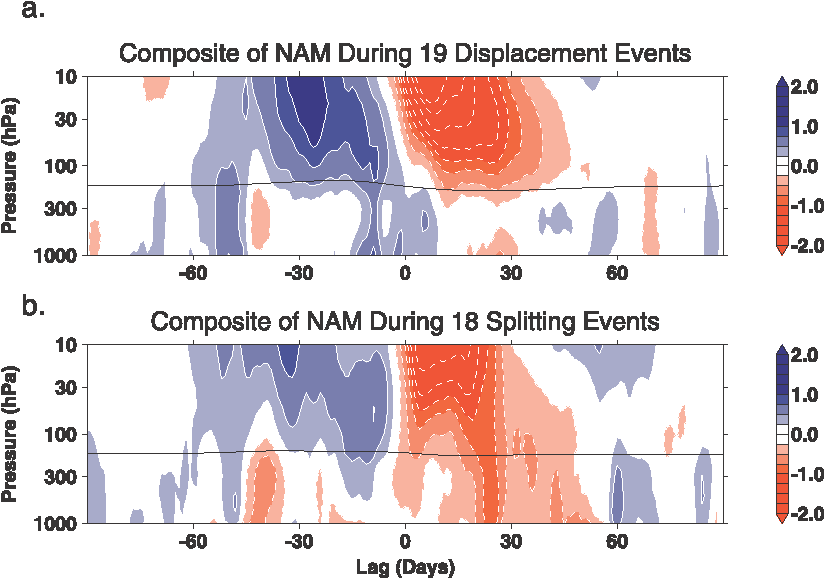
\includegraphics[width=\textwidth]{figures/chapter-intro/M13.pdf}
 \caption[NAM composite from \citet{Mitchell2013}]{Composites of the
   time--height evolution of the NAM during (a) 19 vortex displacement events
   and (b) 18 splitting events. The horizontal line is a composite of the
   thermal tropopause level for the two types of event. Lag 0 shows the onset of
   an event as measured at 10~hPa. Contour intervals are 0.25 and the region
   between $-0.25$ and 0.25 is unshaded. Figure from \citet{Mitchell2013}. }
 \label{fig:M13}
\end{figure}


It has been observed that some SSW events, while appearing to have similar
magnitudes in the stratosphere, have very different signatures in the
troposphere \citep[e.g.,][]{Baldwin2001a,Tomassini2012} (See also the two events
shown in Figure \ref{fig:baldwin_dunkerton}). This issue was addressed by
\citet{Nakagawa2006} and \citet{Mitchell2013}, who compared tropospheric
anomalies following SSWs dominated by wave-1/wave-2 activity and displaced/split
vortex events respectively (these two classifications are related but not
identical: e.g., \citet{Waugh1997}, Section
\ref{sec:moments-introduction}). These studies found stronger stratospheric
anomalies following wave-2/split vortex SSWs than following wave-1/displaced
vortex SSWs.\footnote{Using the method developed in Chapter \ref{cha:moments},
  of the two weak vortex events illustrated in Figure
  \ref{fig:baldwin_dunkerton}, the first is identified as a displaced vortex
  event and the second as a split vortex event. Their tropospheric NAM may
  therefore be expected to be different, although no firm conclusions should be
  reached from the study of just two events.} This result is illustrated in
Figure \ref{fig:M13}, which shows composites of the NAM following the split and
displaced vortex events identified by \citet{Mitchell2013}. It can be seen that
tropospheric anomalies are stronger following split vortex events and persist
for up to two months, while the NAM signal following displaced vortex events
appears not to descend below the tropopause even though its stratospheric
magnitude is greater. \citet{Mitchell2013} went on to link these different NAM
signals to an increase in high-latitude blocking following split vortex events,
and a weaker blocking signal following displaced vortex events. On the other
hand \citet{Charlton2007}, using a different classification method, found
little difference in the tropospheric signals following split and displaced
vortex events. This discrepancy between these studies highlights the importance
of the classification method of split and displaced vortex events (or of
tropospheric variability); an issue which is addressed in Chapter
\ref{cha:moments}.

It is not only mid-winter stratospheric variability which has been suggested to
influence tropospheric weather. \citet{Hardiman2011} found differences
in NH springtime sea-level pressure anomalies following two types of
stratospheric final warming; more radiatively driven final warmings where the
transition to easterlies happens first in the upper stratosphere and descends
with time, and more dynamically driven final warmings where the transition to
easterlies happens first in the midstratosphere.  

A significant limitation of the above observational studies, which employ
composite or correlation analysis, is that they cannot in themselves demonstrate
\emph{causality}. For example, there may be the possibility that a third factor
(such as sea-surface temperatures) affects both the troposphere and stratosphere
separately. To address this, a number of modelling studies have been carried out
which measure the tropospheric response to some imposed stratospheric
perturbation. These are described in the next section.


% extreme events
% splits and displacements
% - + sd blocking incl Martius 2009
% hardiman fws

\subsection{Modelling evidence}
\label{sec:modelling-evidence}
Modelling investigations into a possible stratospheric influence on the
troposphere predate the observational evidence described above. In a general
circulation model (GCM) study, \citet{Boville1984} showed that changes to upper
tropospheric and lower stratospheric zonal mean zonal winds have a significant
effect on mid-troposphere wave fields, although the wind changes imposed in his
model were larger than those in reality. Using more realistic wind variations,
\citet{Jacqmin1985} found the troposphere to be largely insensitive to changes
in the state of the stratosphere. However, several more recent studies using
models with a more realistic representation of stratospheric dynamics, have
found a consistent tropospheric response to an imposed stratospheric torque
\citep[e.g.,][]{Polvani2002,Norton2003, Taguchi2003}. This tropospheric response
is found to resemble the negative phase of the NAO or NAM following a weakening
of the vortex, and as such is consistent with the observational results
discussed in the previous section.

Figure \ref{fig:jung_barkmeijer} shows the results from another such study by
\citet{Jung2006}, who imposed a weakening of the stratospheric polar vortex
using an adjoint method. Differences of zonal-mean zonal wind at four time
periods following the imposition of this forcing are shown for the composite of
60 forecasts. It can be seen that anomalies are initially confined to the
stratosphere but descend to the troposphere after approximately 20
days. \citet{Jung2006} also found surface anomalies associated with this forcing
to resemble the negative phase of the NAO, though with the southern node shifted
slightly eastwards. Interestingly, they found an almost opposite surface
response when a strengthening of the stratospheric polar vortex was
imposed. This indicates that the surface response may be linear, potentially
providing some information about the mechanism responsible for the response, as
discussed in the next section.

\begin{figure}
 \centering
 \noindent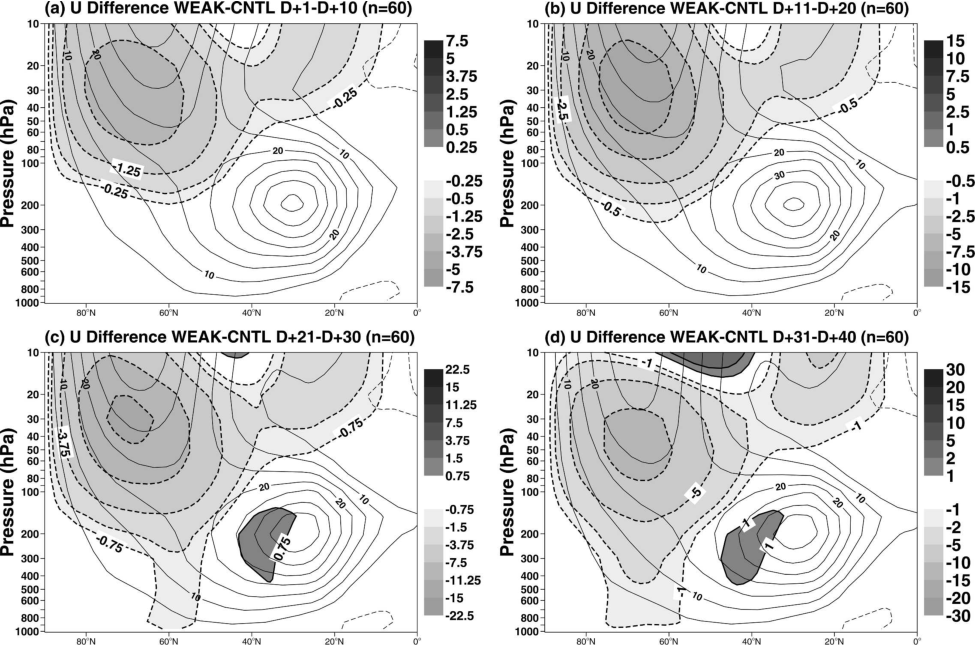
\includegraphics[width=\textwidth]{figures/chapter-intro/Jung_Barkmeijer.pdf}
 \caption[Numerical simulation results from \citet{Jung2006}]{Difference of
   average zonal-mean zonal winds (shading in $\mathrm{m~s^{-1}}$) between the
   weak polar vortex (WEAK) and the control experiment (CNTL) for 10-day
   averages: (a) D +1 to D +10, (b) D +11 to D +20, (c) D +21 to D +30, and (d)
   D + 31 to D +40. Shown is the average over 60 different cases (40-day
   integrations). Notice that the contour interval for the differences changes
   linearly with the forecast range. Also shown are zonal-mean zonal winds from
   the control integration (contour interval is $\mathrm{5~m~s^{-1}}$). Figure
   from \citet{Jung2006}.}
 \label{fig:jung_barkmeijer}
\end{figure}

This tropospheric response to an imposed torque was shown to also operate on
long time scales by \citet{Scaife2005}. They found that when a long-term
acceleration of the stratospheric polar vortex was imposed from the
1960s--1990s, in line with observations, their model more faithfully reproduced
the long-term trend towards a more positive phase of the NAO over this time. It
is however, important to note that this does not necessarily imply that
stratospheric changes were driving the trend in reality.

In contrast to the studies above, which have calculated the tropospheric
response to an imposed stratospheric forcing, \citet{Simpson2011} removed the
stratospheric influence by damping the polar stratosphere to a climatological
seasonal cycle. In doing so, they found that the effect of the stratosphere is
to lengthen SAM timescales\footnote{The SAM/NAM timescale is defined as the lag
  (in days) for its autocorrelation to fall by 1/$e$.} during the austral late
spring/early summer, and to lengthen NAM timescales during the boreal
winter-spring.

A criticism of studies with an imposed damping or torque is that they may not be
simulating a balanced, realistic, or physical state (for instance, the imposed
torque may not conserve angular momentum). As such, several studies have taken
place using free-running GCMs. \citet{Plumb2003} found using a simple
free-running stratosphere-only model that descending annular mode-like signals
of the kind shown in Figure \ref{fig:baldwin_dunkerton} can be simulated only by
changing the forcing at the lower boundary. They therefore conclude that
observations of this kind do not necessarily indicate a downwards influence from
the stratosphere. However, \citet{Gerber2008} undertook a similar study,
comparing relatively simple GCM simulations with varying representations of the
stratosphere. They altered the strength and variability of the stratospheric
polar vortex independently of the troposphere by varying the stratospheric lapse
rate, finding that simulations with a more variable polar vortex also had longer
timescales of the tropospheric NAM (a result similar to that of
\citet{Simpson2011}, although using a free-running model). This lengthened
timescale, in turn, was related to the long-lived tropospheric anomalies
following SSWs. Using the same model, \citet{Gerber2009} performed a series of
ensemble forecasts of model-simulated SSW events. They compared events in which
the initial tropospheric NAM was negative and positive, finding a negative NAM
to be much more likely following the SSW event in both cases. Hence, they
conclude that the stratosphere does indeed exert a significant downwards
influence on the troposphere in their model.

A further class of model investigation has been to compare models with a
well-resolved stratosphere with models with a coarser stratospheric resolution;
known as `high-top' and `low-top' models respectively \citep{Huebener2007,
  Sigmond2008, Cagnazzo2009, Sassi2010, Scaife2011, Charlton-Perez2013}
(discussed in greater detail in Section \ref{sec:models_introduction}). These
have all indicated a more realistic representation of tropospheric variability
and long-term trends is achieved with improved vertical
resolution. Additionally, in a case study of the cold European winter
2005--2006, \citet{Scaife2008} found increased blocking activity in a model with
greater stratospheric resolution. On the other hand, in a multi-model comparison
of blocking, \citet{Anstey2013} found a stronger relationship between blocking
frequency and upper-troposphere/lower-stratosphere vertical resolution than with
model lid height. Overall, large biases remain in models' representation of
blocking. A difficulty of these studies is that there are often several
differences between high- and low-top models besides their vertical resolution
(such as their parametrisation schemes), so it is difficult to pin down any
differences between the simulations to a stratospheric influence
alone. \citet{Hardiman2012a} attempted to address this issue by comparing model
simulations which differ only in their vertical resolution above 15~km. They
found the climatology and trends of surface temperature to be largely
insensitive to the increased vertical resolution, although stronger surface
anomalies following SSWs and a more realistic trend in the NAO were found in the
high-top model.

Several studies have investigated the influence of the stratosphere on the skill
of medium-range forecasts (also discussed in Section
\ref{sec:seas-introduction}). These have demonstrated improvements in the
medium-range predictive skill of high-top relative to low-top models
\citep{Marshall2010,Roff2011}, and enhanced predictability when forecasts are
initialised at the time of anomalously negative stratospheric NAM or SSWs
\citep{Kuroda2008,Mukougawa2009,Sigmond2013}. These studies therefore further
indicate a downwards influence of stratospheric variability on the troposphere. 



% Scaife and Knight cold 2006
% Simpson timescales
% blocking in models
% forecasts e.g. Charlton

\subsection{Mechanisms}
\label{sec:mechanisms}

The results described in the previous two sections provide strong evidence that
the stratosphere does indeed exert a significant influence on tropospheric
weather and climate. Even so, may uncertainties about the exact nature of the
influence remain; observational studies are always open to the criticism that
they do not demonstrate causality, and modelling studies that they contain large
model biases or are simulating an unrealistic scenario. A coherent picture of
stratosphere-troposphere coupling also requires a physical understanding of the
mechanism by which this takes place. Several such mechanisms have been proposed,
and are briefly described below:



\bigskip\noindent\textsc{Radiative effects.} It is well known that stratospheric (particularly
lower-stratospheric) temperature increases following SSWs lead to increasing
downwelling longwave radiation entering the troposphere.  \citet{Ramanathan1977}
argued that this warming could reduce the available potential energy accessible
to tropospheric eddy activity. Similarly, the stratospheric cooling associated
with ozone depletion leads to a reduction in downwelling longwave radiation
entering the troposphere \citep{Forster1997a}. \citet{Grise2009} used a
radiative transfer model to asses the impact of these radiation changes, finding
a significant impact on surface polar temperatures, although they did not assess
the circulation response. Indeed, relatively few studies have assessed the
impact of radiative processes in stratosphere-troposphere coupling in the light
of more recent observations. Despite this, it is unlikely that radiative effects
play a large role in the observed stratosphere-troposphere coupling since
relatively realistic coupling can be simulated in a model lacking interactive
ozone or a detailed radiation scheme.

\bigskip\noindent\textsc{Baroclinic instability.} The growth rate of baroclinic
eddies is related to the vertical shear in zonal wind throughout the troposphere
\citep{Eady1949}. Some studies have suggested that lower stratospheric zonal
wind anomalies which penetrate into the upper troposphere affect this vertical
wind shear, and so the growth of baroclinic eddies \citep{Wittman2007,
  Chen2008}. Hence, we may expect reduced tropospheric eddy activity at
mid-to-high latitudes following SSWs, due to weaker lower stratosphere/upper
troposphere zonal winds. \citet{Scaife2011} also used this relationship to
demonstrate that an increase in European winter storminess and equatorward shift
in the North Atlantic storm track projected under climate change are consistent
with a weakening and equatorward shift of the stratospheric polar vortex. It is
less clear whether the change in baroclinic eddy activity is sufficient to lead
to the annular mode signals of the kind shown in Figure
\ref{fig:baldwin_dunkerton}, although tropospheric eddies have been demonstrated
to be important in driving annular mode variability \citep{Limpasuvan1999}.

\bigskip\noindent\textsc{Downward control.} Under steady-state or time-mean
conditions, the `downward control' principle of \citet{Haynes1991} shows that
the streamfunction, $\psi$, of the TEM residual circulation is given by
\begin{equation}
  \psi(\phi,z) =
  \int_z^{\infty}\left(\frac{\rho_0a\overline{\mathcal{F}}\cos^2\phi}{\partial\overline{m}/\partial\phi}\right)_{\phi=\phi(z')}\mathrm{d}z'\, ,
\end{equation}
where $\overline{\mathcal{F}}$ is the total wave driving term from Equation
\ref{eq:zonal_momentum}, and
$\overline{m}=a\cos\phi(\overline{u}+a\Omega\cos\phi)$ is the angular momentum
per unit mass. Strictly, the integration is along a line of constant angular
momentum, but this is approximated as vertical (an approximation which breaks
down near the equator). Hence, it can be seen that under these conditions the
residual circulation at a given altitude depends only on the wave drag above
that altitude.

This relation therefore shows that circulation induced by stratospheric wave
drag extends to the Earth's surface, although it should be noted that the above
assumptions (particularly steady-state) do not strictly hold in the real
atmosphere. \citet{Thompson2006} suggested that this induced residual
circulation (or `balanced response') is sufficient to explain the observed
stratosphere-troposphere coupling. Others, however, have argued that the
observed annular mode-like tropospheric response cannot be generated in the
zonal-mean framework of downward control, necessitating feedbacks involving
tropospheric eddies \citep{Kushner2004, Song2004}.


\bigskip\noindent\textsc{Planetary wave reflection/refraction.} The critical
surface formed
in the stratosphere during SSW events acts to reflect upward-propagating
planetary waves, as described in Section
\ref{sec:planetary-waves}. \citet{JudithPerlwitz2003} argued that these
reflected planetary waves re-enter the troposphere and affect the tropospheric
wave structures, leading to the observed tropospheric response. \citet{Shaw2010}
have further suggested that strong two-way coupling exists in the presence of
both a vertical reflecting surface and a strong meridional PV gradient, which
act to create a wave guide.

Other studies have suggested that it is the refraction of planetary waves at
lower levels, in the upper-troposphere/lower stratosphere (UTLS), that is most
important for communicating stratospheric anomalies to the surface
\citep{Limpasuvan2000,Hartmann2000}. Indeed, \citet{Chen1992} showed that
planetary wave propagation is very sensitive to small changes in this region
(also discussed by \citet{Haynes2005}).

\bigskip\noindent\textsc{Local adjustment to PV anomalies.} Under the QG
approximation, PV anomalies, $q'$, can be related to geopotential height
anomalies, $Z'$, through
\begin{equation}
  q' = \mathcal{L}(Z')\, ,
\end{equation}
where $\mathcal{L}$ is a linear Laplacian-like operator \citep{Charney1962}. It
follows that the geopotential anomalies (and with QG approximations, other
dynamical fields) associated with a given PV anomaly can be derived by inverting
this operator. The geopotential height anomalies associated with a given PV
anomaly can be thought to be localised in that they decay with a typical
vertical and horizontal scales $H$ and $L$, which are the scale height and
horizontal scale of the QG flow respectively\footnote{It follows from this that
  PV-inversion is global in the sense that knowledge of the PV field everywhere
  is needed in order to fully determine the other dynamical fields.}. In the
case of lower-stratospheric PV anomalies, their influence may therefore extend
to the troposphere. \citet{Hartley1998} and \citet{Black2002} performed such
PV-inversions to calculate the tropospheric effect of stratospheric PV
anomalies. They found stratospheric PV anomalies to contribute significantly to
anomalies at the tropopause, which extend to the Earth's surface.

\begin{figure}
  \centering
  \noindent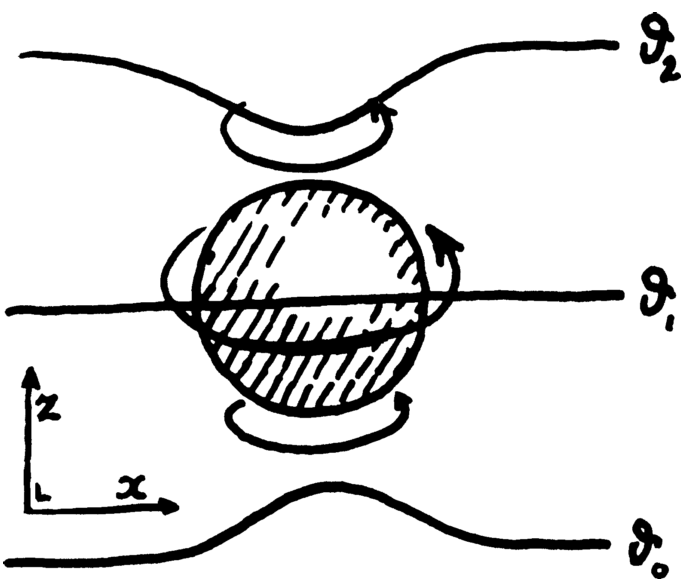
\includegraphics[width=0.4\textwidth]{figures/chapter-intro/ambaum_hoskins.png}
  \caption[Schematic from \citet{Ambaum2002}]{Schematic of the bending of
    isentropic surfaces (labelled $\theta_0$, $\theta_1$, and $\theta_2$) toward
    a positive potential vorticity anomaly. The arrows represent winds
    associated with the potential vorticity anomaly, becoming weaker away from
    the anomaly. Figure from \citet{Ambaum2002}.}
  \label{fig:ambaum_hoskins}
\end{figure}

It can be argued that PV-inversion does not constitute a `mechanism' since it is
not a time-dependent relationship and does not imply a direction of
causality. However, \citet{Ambaum2002} developed a physical mechanism analogous
to PV-inversion, as follows. Anomalies of PV act to bend isentropic surfaces
\citep{Hoskins1985}, as illustrated in Figure \ref{fig:ambaum_hoskins}. At high
latitudes, the tropopause lies approximately on a potential vorticity surface,
also the potential temperature of the tropopause will be conserved for adiabatic
changes (Section \ref{sec:planetary-waves}). Hence, the tropopause will also
bend in the presence of a stratospheric potential vorticity anomaly; moving
upwards for a positive anomaly, and downwards for a negative anomaly. This
deformation of the tropopause will then lead to hydrostatic and geostrophic
adjustment of the tropospheric column below, which can be thought of in terms of
the conservation of angular momentum, with a stretched tropospheric column
leading to an increase of vorticity and lower pressure. It is therefore be
expected that a strengthening of the stratospheric polar vortex would be
associated with negative sea-level pressure anomalies over the pole, and a
weakening with positive pressure anomalies, which is consistent with the
observed annular mode relationships (Section \ref{sec:observ-evid}).

Importantly, \citet{Ambaum2002} noted a stratosphere-leading time-lagged
relationship between the strength of the stratospheric polar vortex, the
tropopause height and the NAO, with the stratosphere acting to integrate the
NAO. This therefore represents a time-dependent and causal mechanism for
stratosphere-troposphere coupling.
\begin{center}
\line(1,0){250}
\end{center}


The above list is not exhaustive but represents the most prominent proposed
mechanisms. It is clear that several of these mechanisms are not mutually
exclusive and so it is likely that more than one is at work in the real
atmosphere. Furthermore, a difficulty in distinguishing the relative importance
of the different mechanisms is that they are largely consistent with
observations, particularly in the tropospheric annular mode response to changes
in stratospheric polar vortex strength. It is therefore important to identify
situations in which mechanisms make different predictions and test these against
reality and numerical simulations.

One such situation is in the response to zonally asymmetric stratospheric
anomalies. For instance, the planetary wave reflection and downward control
mechanisms are largely sensitive only to zonal-mean quantities. Hence, it might
be expected that under these mechanisms the tropospheric response to two equal
zonal-mean stratospheric anomalies would be the same, even if the anomalies have
different zonal asymmetries. On the other hand, the tropospheric response via
adjustment to PV anomalies would be expected to be local to the stratospheric
anomalies.

It is the aim of Chapters \ref{cha:moments} and \ref{cha:models} to diagnose
zonally asymmetric stratospheric variability, specifically split and displaced
vortex events, in observations and model simulations. Part of the motivation for
this analysis is then to study the tropospheric response in order to test the
relative importance of the above mechanisms.

% Look at Song and Robinson 2004 for basis of mechanisms review
% Radiative Grise, Waugh
% SH coupling T&W


%\begin{figure}
% \centering
% \noindent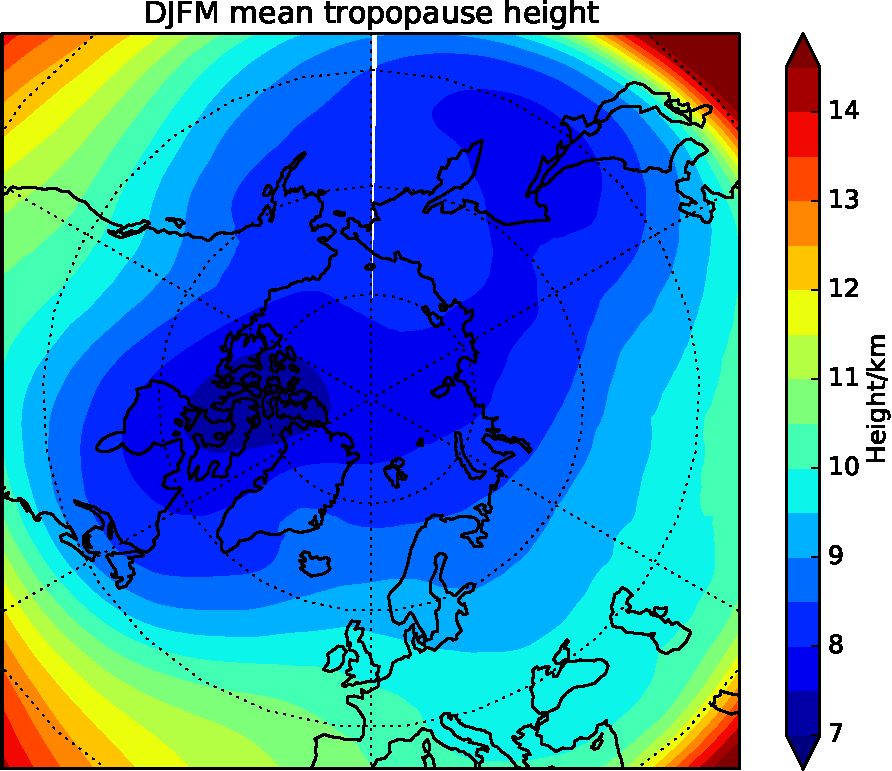
\includegraphics[width=0.5\textwidth]{figures/chapter-intro/mean_tropopause_height.pdf}
% \caption[]{ }
% \label{fig:cmip5_mslp_diff}
%\end{figure}



%%% Local Variables:
%%% mode: latex
%%% TeX-master: "thesis"
%%% End:








\chapter{A geometrical description of vortex variability}
\begin{quotation}
  Much of the work contained in this chapter is based upon \citet{Seviour2013},
  published in \emph{Geophysical Research Letters}, although the analysis
  presented here has been significantly extended.
\end{quotation}

\label{cha:moments}

% To Do: 
% - Discussion of sensitivity of the clustering algorithm
% - Description of dripping paint plot
% - Significance for dripping paint plot
% - CP07 and M13 events in table (or maybe disagreeing events highlighed
%   - plot disagreeing events seperately to check
% - Possibly add seasnal cycle of moment diagnostics with percentiles 



\section{Introduction}
\label{sec:moments-introduction}
A quantitative description of stratospheric polar vortex variability is
desirable for a number of reasons; it allows for the comparison of different
studies, observational data sets, and model simulations, as well as permitting
robust definitions of extreme events.  Traditional methods to quantify vortex
variability have been based on zonal-mean diagnostics, such as the zonal-mean
zonal wind \citep[e.g.,][]{Andrews1987}. This was motivated both by the
simplicity of these diagnostics and the physical reasoning that the strength of
the zonal flow controls the propagation of planetary waves \citep[][Section
\ref{sec:plan-waves-strat}]{Charney1961}. \citet{McInturff1978} provided the
first quantitative definition of SSWs\footnote{In the literature, this is often
  called ``the WMO definition''.} (referred to in that text as ``major
stratospheric warmings'') using zonal mean quantities as below.
\begin{quotation}
\emph{A stratospheric warming can be said to be major if at 10~mb or below the
latitudinal mean temperature increases poleward from 60 degrees latitude and an
associated circulation reversal is observed (i.e., mean westerly winds poleward
of 60$^{\circ}$ latitude are succeeded by mean easterlies in the same area).}
\end{quotation}
A number of variations of this definition have since appeared in the
literature. Most commonly, the temperature gradient criterion has been neglected
and/or zonal wind reversals at a particular latitude (usually $60^{\circ}$N)
used instead of the stricter criterion of a reversal everywhere poleward of
$60^{\circ}$N \citep[e.g.,][]{Labitzke2000, Christiansen2001,
  Reichler2012}. 

Although the reversal of zonal-mean zonal wind is physically relevant for the
propagation of planetary waves, the choice of $60^{\circ}$N and 10~hPa in the
definition of SSWs is less physically significant. Indeed, different numbers of
SSWs are identified if these locations are varied. \citet{Butler2014a} found
that a greater number of events are identified if the threshold is located
either equatorward or poleward of $60^{\circ}$N. Some studies have aimed to
avoid this sensitivity to spatial location by quantifying vortex variability
through empirical orthogonal function (EOF) analysis, using fields over a larger
area. This includes the Northern Annular Mode (NAM) (calculated either from the
three-dimensional geopotential height field \citep{Baldwin2001a} or zonal-mean
geopotential height \citep{Baldwin2009}), EOFs of zonal wind
\citep{Limpasuvan2004}, and vertical profiles of polar cap-averaged temperature
\citep{Kuroda2004}. SSW events are then defined by a threshold in the principal
component of the relevant EOF.

As it has become increasingly recognised that SSWs generally occur as either
split or displaced vortex events, studies have aimed to objectively distinguish
these two types of event. Commonly this has been achieved through Fourier
decomposition of the zonal wave structure. For instance, \citet{Nakagawa2006}
defined SSWs through a polar temperature criterion and then split these events
into two groups depending on whether the 150~hPa Eliassen-Palm (EP) flux prior
to the events was dominated by zonal wavenumber one or two. \citet{Charlton2007}
(hereafter CP07) introduced a new classification method, which does not rely on
Fourier decomposition; first they identified events using the traditional wind
reversal at $60^{\circ}$N, 10~hPa criterion, then they calculated the circulation
around the two largest contours of relative vorticity on the vortex edge. If
these two contours have a circulation ratio of 2:1 or lower the event is
classified as a split, and all other events are automatically classed as
displacements. 

Both Fourier decomposition of the zonal wave structure and the method of CP07
rely on an Eulerian framework, with fields analysed at a fixed spatial
location. \citet{Waugh1997} first applied two-dimensional moment diagnostics
(otherwise known as elliptical diagnostics) to the stratospheric polar vortex to
provide an alternative semi-Lagrangian (or vortex-oriented) framework. These
diagnostics are calculated by fitting an ellipse to a contour and then
determining its properties such as the centre, orientation, aspect ratio, and
area (a further diagnostic, excess kurtosis--a measure of the `peakedness' of
the distribution--was introduced by \citet{Matthewman2009}). This allows the
movement and elongation of the vortex to be quantified. \citet{Waugh1997} also
compared these diagnostics to the traditional Fourier decomposition. He showed
that wave-1 and 2 amplitudes relate most strongly to the displacement and
elongation of the vortex respectively, however, these relationships were not
found to be strong, with correlations of daily values less than 0.5. These weak
relationships were attributed to the fact that planetary wave propagation can be
affected by changes in the meridional PV gradient, even if the vortex shape and
location are fixed. Furthermore, the wave-1 amplitude depends to some extent on
the elongation of the vortex as well as the location of the centre (and
similarly for the wave-2 amplitude). He concluded that it is difficult to
extract quantitative information about the shape and location of the vortex
based on wave amplitudes alone, highlighting the advantages of the moment
diagnostics.

\citet{Hannachi2010} then applied a hierarchical clustering algorithm to daily
values of the area, centroid latitude, and aspect ratio diagnostics and found
that the vortex falls preferably into three clusters corresponding to
undisturbed, split, and displaced states. These groupings were used by
\citet{Mitchell2013} (hereafter M13) to identify split and displaced vortex
events; if the vortex remained in the split or displaced cluster for at least
five consecutive days it was classified as the corresponding
event. Significantly, as discussed in Section \ref{sec:observ-evid}, M13
demonstrated that split vortex events penetrated deep into the troposphere and
resulted in significant surface anomalies, while anomalies associated with
displaced vortex events do not descend far below the tropopause. This is in
agreement with \citet{Nakagawa2006} who found tropospheric anomalies to be
larger following SSWs with dominant wave 2 amplitude, however, it contrasts with
CP07, who found little difference in the tropospheric impact of split and
displaced vortex events. This highlights the potential importance of the method
of classification of split and displaced vortex events in any study.

In this chapter we wish to develop a method for the classification of split and
displaced vortex events with the following properties:
\begin{itemize}
\item It is based on vortex moment diagnostics.
\item It can be easily applied to a range of data sets, including climate model
  simulations.
\item It is computationally inexpensive. 
\end{itemize}
The motivation for the use of moment diagnostics includes their advantages in
quantifying the shape and location of the vortex, as noted above. This, in turn,
is desirable because the location of the vortex near the tropopause may be
important for understanding the regional tropospheric effect of stratospheric
anomalies \citep[e.g.,][Section \ref{sec:mechanisms}]{Ambaum2002}. Previous
calculations of vortex moment diagnostics have been based on the distributions
of quasi-conservative tracers such as PV on isentropic surfaces
\citep{Mitchell2011} or long-lived tracer (e.g., N$_{2}$O) concentrations
\citep{Waugh1997}. These quantities have strong meridional gradients allowing
for clear determination of the vortex edge \citep{Nash1996}. Unfortunately, many
climate models do not output PV or tracer concentrations, and these are often
computationally expensive or impractical to calculate. As such, we wish to
develop a method which uses geopotential height, a variable which is output by
all contemporary climate models. This effort will also allow us to test the
robustness of the result of M13 regarding the different surface impacts of split
and displaced vortex events using a semi-independent classification method and
extended data set.

The remainder of this chapter is structured as follows. The next section
introduces the necessary theoretical background for the calculation of moment
diagnostics. Section \ref{sec:methodology} describes the methods used for the
classification of split and displaced vortex events, and compares these events
with those determined by M13 and CP07. Section \ref{sec:moments_analysis}
contrasts the surface impacts of split and displaced vortex events calculated
using the new method and discusses potential mechanisms behind any differences. 


% Stratospheric sudden warmings (SSWs) are extreme events in which the strong
% westerly winds that usually dominate the winter polar stratosphere become highly
% disturbed (here, for reasons outlined below, we use the term SSW to encompass a
% wider range of variability than its traditional definition). These events lead
% to the mixing of mid-latitude air into the polar vortex region, causing an
% increase in temperatures by several tens of kelvin over the course of a few
% days. Traditional methods to identify stratospheric sudden warmings (SSWs) have
% relied on either zonal-mean \citep{Andrews1987} or annular mode
% \citep{Baldwin2001a} diagnostics. Neither method explicitly deals with the
% inherent zonal asymmetry in vortex variability. In particular, SSWs are observed
% to occur in one of two manners: displaced vortex events, where the vortex moves
% far from the pole, and split vortex events, where the vortex separates into two
% `child' vortices. These two types have a very different spatial structure and
% evolution timescale \citep{Matthewman2009}. Displaced and split vortex events
% are predominantly associated with vertically propagating Rossby waves of
% wavenumber 1 and 2 respectively, and many previous studies have classified SSWs
% based on wavenumber \citep[e.g.][]{Nakagawa2006}. However, this method does not
% provide a description of the location of the polar vortex itself, which
% theoretical arguments suggest may be important for understanding
% stratosphere-troposphere coupling \citep{Ambaum2002}. In an improvement to these
% traditional SSW definitions, \citet{Charlton2007} (hereafter CP07) introduced a
% classification in which a split vortex event is identified when two vortices
% with a circulation ratio of 2:1 or higher are present, and all other SSWs are
% automatically classed as displaced vortex events. However, they maintained the
% traditional SSW identification which requires there to be a reversal of the
% zonal-mean zonal wind at 10~hPa and $60^{\circ}$N.

% An increased understanding of stratospheric variability can be gained by using
% vortex-centric diagnostics, such as two-dimensional (2D) vortex moments
% \citep{Waugh1997, Waugh1999, Mitchell2011, Mitchell2011a}, which provide a
% geometrical description of the vortex and have no reliance on zonal-mean
% properties. Using a classification based on these diagnostics,
% \citet{Mitchell2013} (hereafter M13) identified a greater number of SSWs than
% CP07. This is primarily because they did not use a zonal mean threshold
% criterion. Importantly, M13 also demonstrated that split vortex events
% penetrated deep into the troposphere and resulted in significant surface
% anomalies, while anomalies associated with displaced vortex events do not
% descend far below the tropopause. Their result supported a similar conclusion by
% \citet{Nakagawa2006}, who found that the impact of events associated with an
% enhanced upward flux of wavenumber-2 planetary waves was more likely to reach
% the surface. These results underline the need to correctly identify the precise
% type of SSW, in order to understand stratosphere-troposphere coupling within
% climate models.

% Distinguishing between displaced and split vortex events using the method of M13
% requires the use of potential vorticity (PV), which is not commonly output by
% climate models. For this reason, previous attempts to apply PV-based techniques
% in a multi-model study have led to the majority of models being excluded
% \citep{Mitchell2012a}. Furthermore, their method used a hierarchical clustering
% technique \citep{Hannachi2010}, which is very sensitive to the exact shape of
% the distribution of vortex variability, so is unsuitable for application to a
% range of models with different climatologies. In this chapter, we develop an
% improved method which; (a), is based on the geometry of the vortex, but requires
% only the 10~hPa geopotential height; and (b), identifies events using a simple
% threshold instead of a clustering technique. We apply this new method to the
% ERA-40 and ERA-Interim reanalysis datasets and demonstrate that the method
% captures a similar number of events which are in good agreement with, and at
% least as extreme as, those of M13.

\section{Vortex moment diagnostics}
\label{sec:vort-moment-diagn}

The moments, $M_{n}$, of a one-dimensional distribution can be classified by
their order, $n$, and provide familiar parameters. These are the area under the
distribution (0th order), mean (1st order), variance (2nd order), skewness (3rd
order), and kurtosis (4th order), given by
\begin{equation}
M_{n} = \int_{S} x^{n}f(x)~\mathrm{d}x \, ,
\end{equation}
where $S$ represents the extent of the distribution, $f(x)$, to be integrated
over. The extension of this for a two-dimensional distribution is
straightforwardly
\begin{equation}
M_{nm} = \iint_{S} x^{n}y^{m}f(x,y)~\mathrm{d}x\mathrm{d}y \, ,
\label{eq:2D_moment}
\end{equation}
where the order of the moment is now defined as $m+n$, meaning it is possible to
have different diagnostics with the same order (e.g., $M_{01}$,
$M_{10}$). Although these diagnostics can be further extended to three
dimensions, this has been demonstrated to be highly computationally expensive
\citep{Li1994}, and would require assumptions about the lower and upper bounds
of the vortex region. We therefore calculate two-dimensional moment diagnostics
for the stratospheric polar vortex on quasi-horizontal surfaces. We use two
variables; geopotential height ($f(x,y) = Z(x,y)$) on the 10~hPa pressure level,
and potential vorticity ($f(x,y) = q(x,y)$) on the 850~K potential temperature
(isentropic) surface, which lies close to 10~hPa. Following \citet{Waugh1997},
the calculation of moment diagnostics is simplified by transforming the
spherical data $q(\phi,\lambda)$ and $Z(\phi,\lambda)$, where $\phi$ is latitude
and $\lambda$ longitude, to Cartesian coordinates using the polar stereographic
projection
\begin{equation}
x = \frac{\cos\lambda\cos\phi}{1 \pm \sin\phi}\, , \quad
y = \frac{\pm\sin\lambda\cos\phi}{1 \pm \sin\phi}\, , 
\end{equation}  
where the positive sign is used in the NH and negative in the
SH.

In order to calculate moment diagnostics for the stratospheric polar vortex we
must first isolate the vortex region by defining the vortex edge. Different
methods have previously been used for this calculation; \citet{Waugh1999} used
the mean PV at the maximum of the mean meridional PV gradient, while
\citet{Matthewman2009} defined the vortex edge on a daily basis, using the
average value of PV poleward of $45^{\circ}$N nine days before the onset of a
SSW (their SSWs were defined by zonal-mean zonal wind reversal, as in CP07). A
more complex method due to \citet{Nash1996}, starts by transforming PV to
`equivalent latitude' \citep{Butchart1986} coordinates, before defining the
vortex edge as the position of the largest gradient in a plot of PV against
equivalent latitude. This method was applied in \citet{Mitchell2011} to
calculate the vortex edge. 

None of the three methods outlined above are found to be appropriate for the
present study. We wish to directly compare the PV and geopotential
height-derived moments, but the methods of \citet{Waugh1999} and
\citet{Nash1996} rely on meridional gradients in PV and so may not be
transferable to geopotential height. Furthermore, the method of
\citet{Matthewman2009} is impractical because we wish to define the events from
the moment diagnostics, so will not know their dates before
calculation. Instead, we pick a simple definition; PV ($q_{b}$) or geopotential
height ($Z_{b}$) on the vortex edge is defined as the value of the
December-March (DJFM) mean at $60^{\circ}$N for the NH and the
June-September (JJAS) mean at $60^{\circ}$S for the SH. This is
seen to lie close to contours defined by the above methods, and results are
insensitive to small changes in the latitude chosen.

Having defined the vortex edge, we extend the method \citet{Matthewman2009} to
isolate the vortex region by introducing a transformed PV field, $\hat{q}$,
given by
\begin{equation}
 \hat{q}(x,y) = 
 \begin{cases}
   q(x,y) - q_{b} & \text{if $q(x,y) > q_{b}$} \, , \\
   0 & \text{if $q(x,y) \leq q_{b}$} \, , 
 \end{cases}
\end{equation}
and similarly for geopotential height 
\begin{equation}
 \hat{Z}(x,y) = 
 \begin{cases}
   Z(x,y) - Z_{b} & \text{if $Z(x,y) < Z_{b}$} \, , \\
   0 & \text{if $Z(x,y) \geq Z_{b}$} \, . 
 \end{cases}
\end{equation}
By substituting $f(x,y) = \hat{q}(x,y)$ or $f(x,y) = \hat{Z}(x,y)$ in equation
\ref{eq:2D_moment} it is then possible to calculate the moment diagnostics. The
zeroth order moment diagnostic, $M_{00}$ can be used to define the `equivalent
area', $A_{\mathrm{eq}}$ \citep{Matthewman2009}, as
\begin{equation} 
A_{\mathrm{eq}} = \frac{M_{00}}{q_{b}}\quad \text{or} \quad A_{\mathrm{eq}} = \frac{M_{00}}{Z_b}\, ,
\end{equation}
depending on whether PV or geopotential height based diagnostics are
calculated. Because $M_{00} \approx Aq$, where A is the vortex area, the
equivalent area can be considered a measure of both vortex strength and
area. The first order moment diagnostic can be used to calculate the vortex
centroid,
\begin{equation}
(\bar{x}, \bar{y}) = \left( \frac{M_{10}}{M_{00}}, \frac{M_{01}}{M_{00}} \right)
\, . 
\end{equation}

In order for higher order moment diagnostics to be useful, the moment equation
(\ref{eq:2D_moment}), must be transformed to the \emph{centralised moment}
form \citep{Hall2005}. This calculates moments relative to the vortex centroid,
and is given by
\begin{equation}
J_{mn} = \iint_{S} f(x,y)(x-\bar{x})^n(y-\bar{y})^m~\mathrm{d}x\mathrm{d}y \, .
\end{equation}
Two useful parameters can be derived from the second-order centralised moment
diagnostics, the vortex orientation, $\psi$ (defined as the angle between the
major axis of the ellipse and the $x$-axis) and the aspect ratio, $r$ (defined
as the ratio of the lengths of the major to minor axes), given by
\begin{equation}
\psi = \frac{1}{2} \tan^{-1} \left( \frac{2J_{11}}{J_{20}-J_{02}} \right) \, ,
\end{equation}
\begin{equation}
r = \left| \frac{(J_{20}+J_{02})+\sqrt{4J_{11}^2+(J_{20}-J_{02})^2}}
  {(J_{20}+J_{02})-\sqrt{4J_{11}^2+(J_{20}-J_{02})^2}} \right|^{1/2} \, .
\end{equation}
Using the area, centroid, orientation, and aspect ratio, the \emph{equivalent
  ellipse} can be uniquely defined. Figure \ref{fig:displaced_ellipse} shows the
equivalent ellipse calculated from both PV and geopotential height fields over a
16-day period centred on a displaced vortex event (classified using the method
in Section \ref{sec:methodology}). It can be seen that the equivalent ellipse
provides a qualitatively good fit to the vortex, although this is less good in
Figures \ref{fig:displaced_ellipse}(c,f) when the vortex becomes less elliptical
and filamentation occurs. Greater fine-scale structure and filamentation is
visible in the PV field due to its quasi-conservative properties, however
reasonable agreement can be seen between the PV and geopotential height
ellipses. 

\begin{figure}
 \centering
 \noindent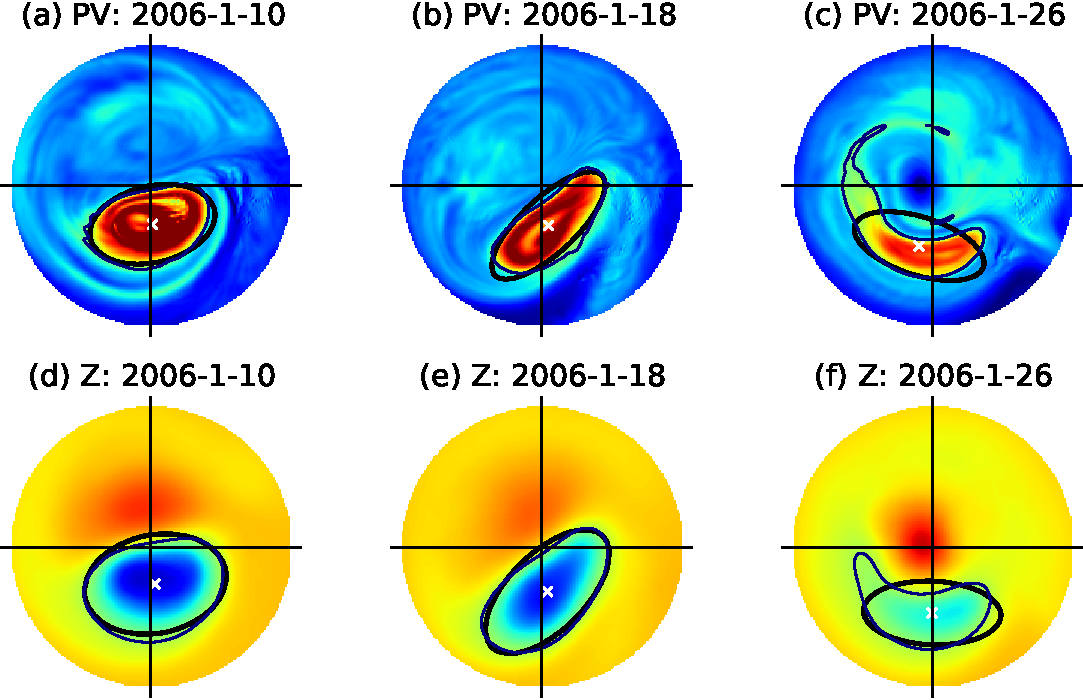
\includegraphics[width=\textwidth]{figures/chapter-moments/PV_GPH_2006.pdf}
 \caption[Equivalent ellipse for a displaced vortex event.]{PV on the 850~K
   $\theta$ surface (a,b,c) and geopotential height at 10~hPa (d,e,f) 8 days
   before (a,d), at onset (b,e), and 8 days following the onset (c,f) of a
   displaced vortex event. Contours of $q_{b}$ and $Z_{b}$ are shown in thin
   black lines, the equivalent ellipse in a thick dark line, and its centroid
   with a white cross. Data are transformed to Cartesian coordinates with a
   polar stereographic projection.}
 \label{fig:displaced_ellipse}
\end{figure}

Equivalent ellipses for an example of a split vortex event are shown in Figure
\ref{fig:split_ellipse}. It can be seen that after the vortex has separated the
equivalent ellipse becomes less physically significant, as it spans the two
vortices. \citet{Matthewman2009} introduced the 4th order moment diagnostic,
``excess kurtosis'', in order to identify splits of the polar vortex; it is
given by
\begin{equation}
\kappa_4 = M_{00}\frac{J_{40}+2J_{22}+J_{04}}{(J_{20}+J_{02})^2}-\frac{2}{3}\left[\frac{3r^4+2r^2+3}{(r^2+1)^2}\right]\,.
\end{equation}
This has the property of being negative for a vortex with a ``pinched'' shape,
zero for a perfectly elliptical vortex, and positive for a vortex with a strong
central core. When negative kurtosis was detected \citet{Matthewman2009} split
the PV field into two regions along the minor axis of the equivalent ellipse and
re-calculated moment diagnostics for the vortices in these regions separately.

In this study we do not make use of the excess kurtosis or calculate separate
diagnostics for split vortices for three reasons. First, as a 4th order
diagnostic it is a highly skewed variable, making its use in event
classification problematic (this was also found by
\citet{Hannachi2010}). Second, this procedure is more computationally expensive,
requiring about three times the number of calculations during split vortex
events. Third, kurtosis is highly sensitive to horizontal resolution
\citep{Mitchell2011}, and so may not be a suitable diagnostic in the comparison
of climate models with different resolutions. Hence, we calculate single moment
diagnostics even when the vortex has split, but bear in mind that these may not
represent the properties of any real vortex.

Code for the calculation of moment diagnostics using the method described in
this section is available from
\url{https://github.com/wseviour/vortex-moments}. Additionally, a comparison of
aspect ratio and centroid latitude with zonal wavenumber amplitudes is given in
Section \ref{sec:comp-zonal-wave}.

\begin{figure}
 \centering
 \noindent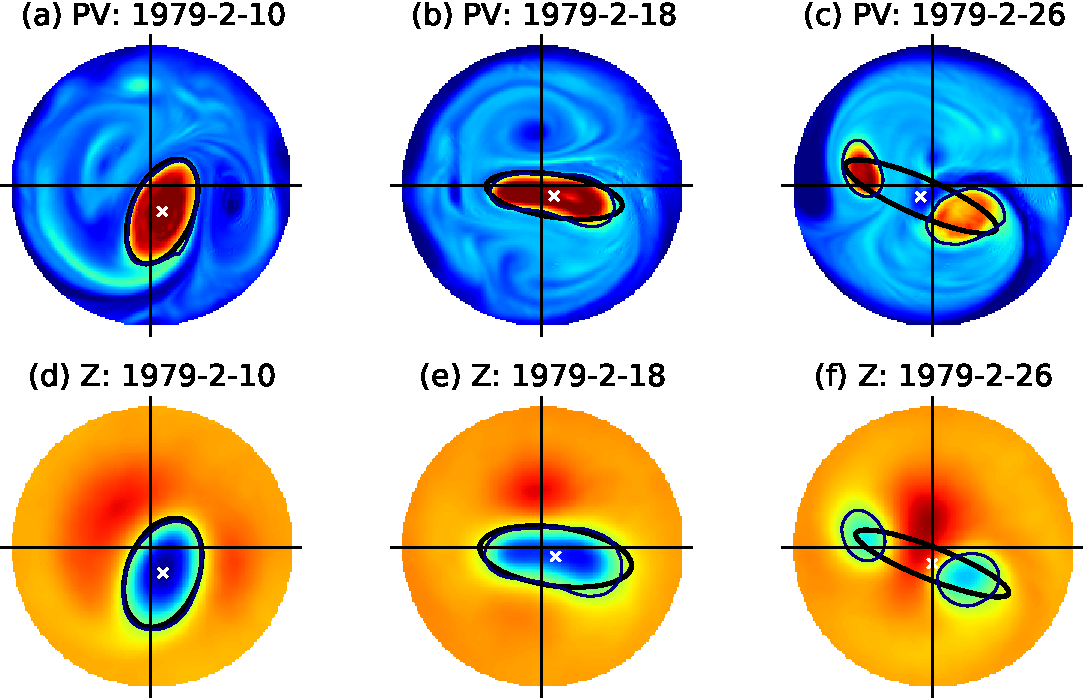
\includegraphics[width=\textwidth]{figures/chapter-moments/PV_GPH_1979.pdf}
 \caption[Equivalent ellipse for a spit vortex event.]{As Figure
   \ref{fig:displaced_ellipse} but for a split vortex event.}
 \label{fig:split_ellipse}
\end{figure}


\section{Data and methods}
\label{sec:methodology}

\subsection{Reanalysis data}
\label{sec:reanalysis-data}
For the analysis in this chapter NH winter daily-mean data for
December-March (DJFM) are employed from the European Centre for Medium-Range
Weather Forecasts (ECMWF) reanalyses. The ERA-40 data set \citep{Uppala2005} is
used from 1958-1978 and ERA-Interim \citep{Dee2011} from 1979-2009. The
combination of these two data sets is chosen in order to maximise the total
number of years entering the analysis (ERA-40 runs only to 2002), as well as to
compare results from the more recent ERA-Interim with previous studies using
only ERA-40, such as \citet{Charlton2007} and \citet{Mitchell2013}.

ERA-Interim is similar to ERA-40 but uses a four-dimensional variational data
assimilation system (4D-Var) as opposed to the 3D-Var system used in ERA-40. It
also has higher horizontal and vertical resolution, improved humidity analysis,
model physics, data quality control, bias handling and other improvements as
noted in \citet{Simmons2007}. The majority of observational data for the
stratosphere entering both reanalyses are from radiosonde and satellite
measurements. It is important to note that in the pre-satellite era (1958-1971)
observations in the stratosphere were much more sparse, leading to greater
errors in reanalyses during this time \citep{Uppala2005}.

A number of studies have evaluated the stratospheric circulation in ERA-40 and
ERA-Interim against other observations or reanalyses. \citet{Randel2004} found
ERA-40 to closely match measurements of the zonal stratospheric circulation
derived from radiosonde, rocketsonde and lidar
measurements. \citet{Karpetchko2005} found that the representation of the polar
vortices in ERA-40 agrees well with the NCEP/NCAR reanalysis, and CP07
demonstrated that this also holds for the occurrence of
SSWs. \citet{Seviour2012} showed that the strength of the stratospheric
meridional mean stratospheric circulation in ERA-Interim agrees well with
previous reanalysis, but that the residual vertical velocity is more smoothly
represented.

In order to perform a consistent analysis across the two data sets, ERA-Interim
data is linearly interpolated to the lower resolution ERA-40
($1.125^{\circ} \times 1.125^{\circ}$) Gaussian grid. PV is also interpolated
from pressure levels to the 850~K isentropic surface (which lies close to
10~hPa), as this quantity has the property of being conserved under adiabatic
flow. Both in the calculation of the vortex edge (climatological mean $q$ or $Z$
at $60^{\circ}$N/S) and the moment diagnostics themselves, no clear jumps were
seen between ERA-40 and ERA-Interim data sets. As such, the two are considered
together with no bias corrections. For the remainder of this thesis, this
combined ERA-40 and ERA-Interim data set is referred to as \emph{ERA}.


\subsection{Moment diagnostic calculation}
\label{sec:vort-geom-calc}

In order to calculate the moment diagnostics, the values of PV and geopotential
height on the vortex edge ($q_b$ and $Z_b$) must first be determined. These are
the $60^{\circ}$N DJFM/$60^{\circ}$S JJAS mean values of PV at 850~K ($q_{850}$)
and 10~hPa geopotential height ($Z_{10}$) respectively. They are found to be
$q_b = 460$~PVU ($\mathrm{1~PVU = 10^{-6}~Km^2kg^{-1}s^{-1}}$) and
$Z_b = 30.2$~km for the NH, and $q_b = 618$~PVU and $Z_b = 29.0$~km for the
SH. Using these values the moment diagnostics are calculated from ERA data for
1958--2009 using the method described in Section \ref{sec:vort-moment-diagn}.

As discussed in Section \ref{sec:vort-moment-diagn} the excess kurtosis
diagnostic is not used in the present analysis. In the interests of simplicity,
only the aspect ratio and centroid latitude diagnostics are used to identify
events, and the centroid longitude, orientation and equivalent area are not
used. The aspect ratio and centroid latitude are the most intuitive diagnostics
for this purpose, with a high aspect ratio and poleward centroid latitude
expected during split vortex events, and a low aspect ratio and equatorward
centroid latitude expected during displaced vortex events.

Figure \ref{fig:pv_z_moments_distribution} shows the distributions of these two
quantities calculated from $q_{850}$ and $Z_{10}$ for the NH vortex. The
centroid latitude distributions are almost identical, with a peak near
$80^{\circ}$N which is in agreement with previous studies
\citep{Waugh1999,Mitchell2011}. The aspect ratio distributions have a similar
shape, with a peak at about 1.3, but the PV based diagnostic has a larger
tail. This is because the PV field contains more small-scale filamentary
structures than geopotential height (e.g. Figures \ref{fig:displaced_ellipse}
and \ref{fig:split_ellipse}), making high aspect ratios more likely. As well as
having similar distributions, the time series of the PV and geopotential height
derived diagnostics (not shown) are significantly correlated, with correlation
coefficients of 0.9 for daily centroid latitude and 0.6 for aspect
ratio. Overall, these results suggest that geopotential height-derived moment
diagnostics are appropriate for the identification of split and displaced vortex
events.


\begin{figure}
  \centering
  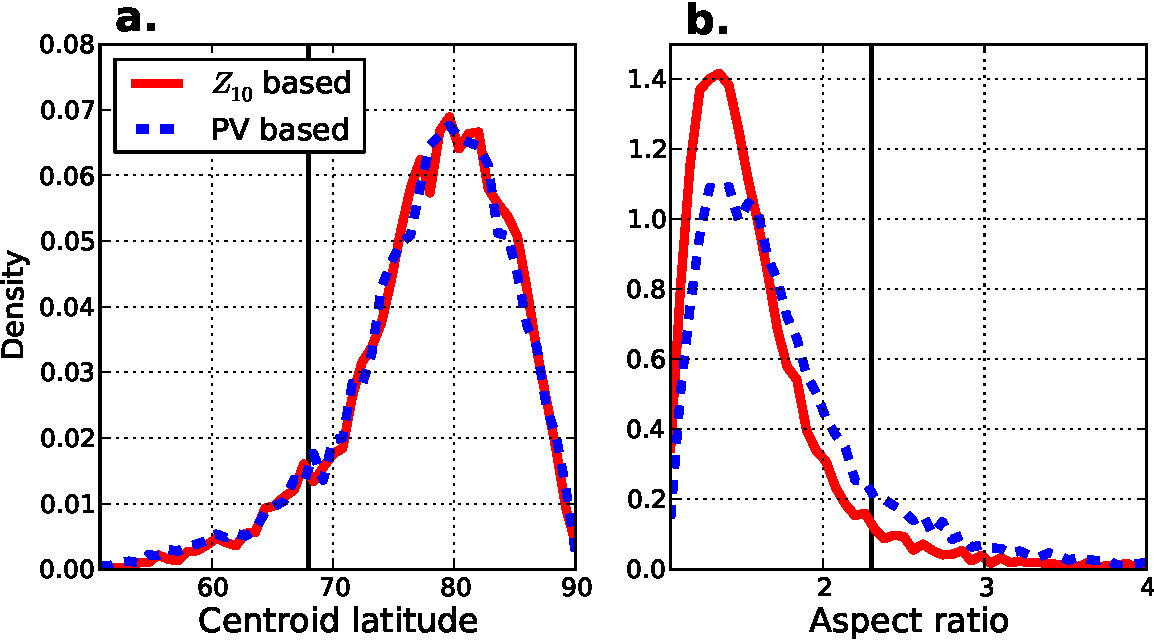
\includegraphics[width=\textwidth]{figures/chapter-moments/moments_distribution_crop.pdf}
  \caption[NH distributions of $Z_{10}$ and PV-based moment
  diagnostics.]{Distributions of the December-March centroid latitude (a) and
    aspect ratio (b), of the NH stratospheric polar vortex over
    1958--2009. Diagnostics are calculated from geopotential height at 10~hPa
    ($Z_{10}$) and potential vorticity at 850~K (PV). Thresholds of
    66$^{\circ}$N in centroid latitude and 2.4 in aspect ratio are used to
    define events, and are indicated by the black vertical lines.}
  \label{fig:pv_z_moments_distribution}
\end{figure}

\begin{figure}
  \centering
  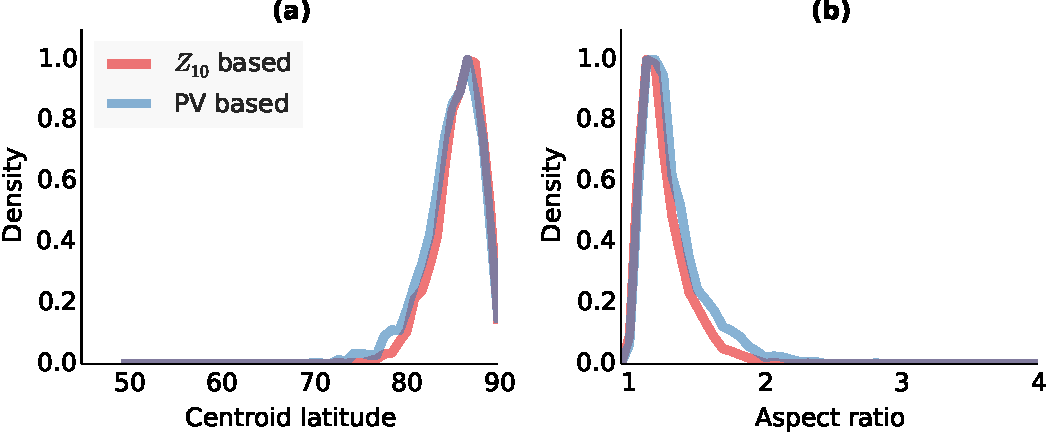
\includegraphics[width=\textwidth]{figures/chapter-moments/moments_distribution_crop_sh.pdf}
  \caption[SH distributions of $Z_{10}$ and PV-based moment diagnostics.]{As
    Figure \ref{fig:pv_z_moments_distribution} but for moment diagnostics
    calculated for the SH stratospheric polar vortex over
    June-September.}
  \label{fig:pv_z_moments_distribution_sh}
\end{figure}

Figure \ref{fig:pv_z_moments_distribution_sh} shows the same distribution as
Figure \ref{fig:pv_z_moments_distribution}, but for the SH vortex aspect ratio
and centroid latitude. As in the case of the Northern Hemisphere, the
geopotential height and PV-based distributions have very similar shapes, with
the PV-based aspect ratio having a slightly larger tail. Comparing the Northern
and SH distributions it can be seen that there is much less variability in both
aspect ratio and centroid latitude in the Southern Hemisphere. This is because
of the reduced planetary wave propagation into the SH stratosphere, in turn a
result of lesser forcing from orography and land-sea temperature contrasts. The
peak in the Southern Hemisphere centroid latitude is at about $86^{\circ}$S; the
same as that found by \citet{Waugh1999}.

A result of this reduced SH vortex variability is that only one SSW has been
observed in the SH (discussed further in Chapter \ref{cha:seas}). The rest of
this chapter relates to the classification and impacts of split and displaced
vortex events and so focuses only on the NH. However, it should be noted that
all the methods below can also be applied to the SH.


\subsection{Event identification}
\label{sec:event-definition}

Previous attempts to identify SSW events have used a clustering method
\citep{K.Coughlin2009,Hannachi2010}. These methods attempt to classify the
vortex state for each day into a number of groups, which may be specified
beforehand or determined by the clustering algorithm. Individual days within the
same cluster should be physically similar, while those in different clusters
distinct. More precisely, clustering aims to maximise the between-cluster
variance while minimising the within-cluster variance. In the case of the
stratospheric polar vortex, clusters may represent, for instance, stable, split,
and displaced states. Events are then typically defined by the vortex persisting
in a particular cluster for a number of days.

\begin{figure}
 \centering
 \noindent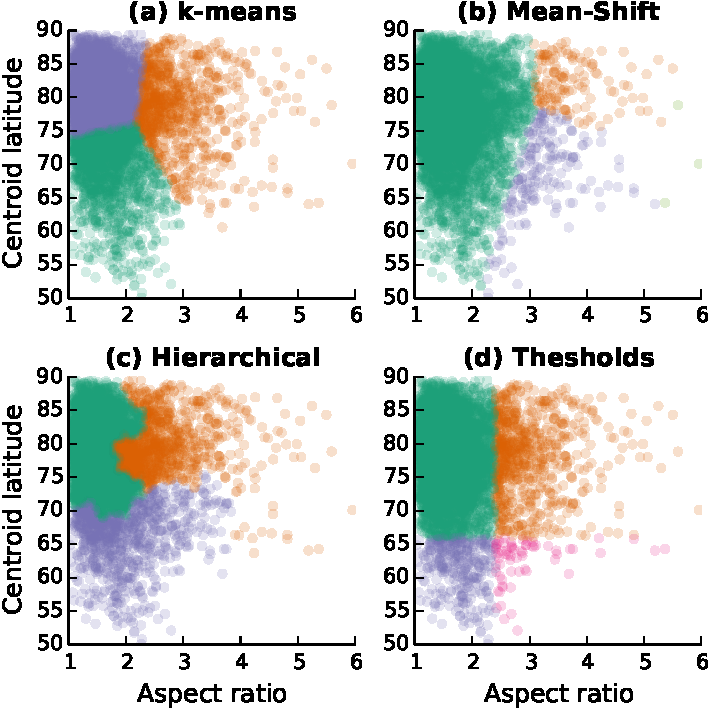
\includegraphics[width=0.7\textwidth]{figures/chapter-moments/clustering.pdf}
 \caption[Clustering algorithms applied to the moment diagnostics.]{Three
   clustering algorithms and a threshold division applied to the moment
   diagnostics in centroid latitude-aspect ratio space. For the $K$-means and
   hierarchical algorithms three clusters were specified. The mean-shift
   algorithm determined the number of clusters to be 4.}
 \label{fig:clusters}
\end{figure}

A large number of clustering algorithms exist, and some may be more appropriate
than others for certain uses. Here, three different algorithms are applied to
the moment diagnostics in centroid latitude-aspect ratio space, and their
outcomes shown in Figure \ref{fig:clusters}(a,b,c). Details of the three
algorithms are given below:

\bigskip\noindent\textbf{(a) \textit{K}-means} clustering requires the number of
clusters, $K$, to be specified beforehand (in Figure \ref{fig:clusters},
$K=3$). The algorithm begins by randomly selecting $K$ data points to be the
centroids of the initial clusters, all other data points are assigned to the
cluster with the nearest centroid. Having assigned the initial cluster
membership, the algorithm proceeds as follows:
\begin{enumerate}[1.]
\item Compute the centroids (the vector means), $\mathbf{\overline{x}}_k$ of
  each cluster.
\item Calculate the qdistance between the current data point, $\mathbf{x}_i$,
  and each of the $K$ $\mathbf{\overline{x}}_k$s. (Various distance measures can
  be used; in Figure \ref{fig:clusters}(a), the Euclidean distance is used).
\item If $\mathbf{x}_i$ is not in the group with the closest mean then reassign
  it to that group, otherwise repeat step 2 for $\mathbf{x}_{i+1}$.
\end{enumerate}
This is repeated until a full cycle through each $\mathbf{x}_i$ produces no
reassignments. An advantage of this method is that it is computationally
efficient, but the major disadvantage is that the number of clusters must be
pre-determined. Several methods exist to estimate the ideal number of clusters,
which generally have the aim of finding the best compromise between minimising
within-cluster variance and maximising between-cluster
variance. \citet{K.Coughlin2009} applied $K$-means clustering to several
variables representing the stratospheric polar vortex. They used the method of
\emph{silhouette values} \citep{Rousseeuw1987} to determine the ideal number of
clusters to be two (representing stable and disturbed vortex states). However,
three clusters has been imposed in Figure \ref{fig:clusters} in order to attempt
to identify stable, split, and displaced states.


\bigskip\noindent\textbf{(b) Mean-shift} clustering aims to discover `blobs' in
a data set. It works by updating candidates for centroids to be the mean of the
points within a given region. That is, given a candidate centroid $\mathbf{x}_i$
for iteration $t$, the candidate is updated according to
\begin{equation}
  \mathbf{x}^{t+1}_{i} = \mathbf{x}^t_i + \mathbf{m}(\mathbf{x}^t_i) \, ,
\end{equation}
where $\mathbf{m}$ is the mean shift vector. This is calculated as
\begin{equation}
  \mathbf{m}(\mathbf{x}_i) = \frac{\sum_{\mathbf{x}_j \in N(\mathbf{x}_i)}K(\mathbf{x}_j-\mathbf{x}_i)\mathbf{x}_j}{\sum_{\mathbf{x}_j
      \in N(\mathbf{x}_i)}K(\mathbf{x}_j-\mathbf{x}_i)} \, ,
\end{equation}
where $K(\mathbf{x}_j-\mathbf{x}_i)$ is a kernel function which determines the
weight of nearby points. Typically, and in Figure \ref{fig:clusters}(b), a
Gaussian kernel is used,
$K(\mathbf{x}_j-\mathbf{x}_i) = e^{-c\|\mathbf{x}_j-\mathbf{x}_i\|^2}$.
$N(\mathbf{x}_i)$ represents the set of points for which
$K(\mathbf{x}_i) \ne 0$. This shifting is repeated until $\mathbf{m}$
converges. Following this calculation, the candidates are then filtered to
remove near duplicates. The greatest advantage of this method is that it
automatically sets the number of clusters, so no prior assumptions about the
data set are required. A disadvantage is that it requires multiple nearest
neighbour searches during each iteration, and so may not be scalable to large
data sets. In Figure \ref{fig:clusters}(b) the number of clusters was determined
to be four (because the fourth cluster is very small it is not easily visible in
Figure \ref{fig:clusters}(b), but represents points with high aspect ratio).

\bigskip\noindent\textbf{(c) Hierarchical} clustering proceeds by calculating a
series of nested clusters. To begin with, all data points are considered each as
a separate cluster and then at each iteration the nearest two clusters are
merged. There are a number of methods to identify the distance between clusters
when those clusters consist of more than one member. Following
\citet{Hannachi2010} the \emph{complete-linkage} method is used here, defining
the distance as the largest distance between members in the two groups. As with
the $K$-means clustering, the number of clusters desired must be pre-determined,
otherwise the algorithm will run to completion with a single cluster consisting
of all data points. Again, many methods exist to determine the optimum number of
clusters. \citet{Hannachi2010} used the gap statistic method
\citep{Tibshirani2001} with vortex area, centroid latitude, and aspect ratio
moment diagnostics, and found a slight preference for three clusters. As such,
three clusters are used in Figure \ref{fig:clusters}(c).


\bigskip Figure \ref{fig:clusters} demonstrates that the three clustering methods
produce very different results. As well as the size and extent of the clusters,
there is also disagreement between this and past studies on the optimum number
of clusters; \citet{K.Coughlin2009} found two clusters using a silhouette values
method, \citet{Hannachi2010} found three clusters using the gap statistic, while
the mean-shift algorithm applied here produces four clusters. Further
sensitivity tests were performed by randomly removing 1\% of the data and
re-calculating the clustering. It was found that very different clusters were
calculated with this small alteration to the data, suggesting that these
clusterings may not be robust if applied to different data sets, such as climate
model simulations. The likely reason for this sensitivity is that the data
itself is not highly clustered; as can be seen in Figure
\ref{fig:pv_z_moments_distribution} no clear bi-modality is present. Rather, it
is more appropriate to view the split and displaced vortex states as the tails
of a distribution rather than distinct clusters or regimes.

For the reasons above, clustering methods are deemed inappropriate for the
present study, and a simpler, more robust, thresholds-based method is
introduced. Days with an aspect ratio $>2.4$ (11\% of all days) or a centroid
latitude $<66^{\circ}$N (5\% of all days) are classified as split and displaced
states respectively. A small number of days lie beyond both thresholds, and
these are classified as a mixed state (1\% of all days). The vast majority of
days (83\%) lie in the stable state, where neither threshold is exceeded. The
choice of thresholds is somewhat subjective but the results presented below are
not sensitive to the exact choice of threshold. They were chosen to give a
similar frequency of split and displaced vortex events (identified using the
method below) as CP07 and M13. 

\citet{Mitchell2011} found that above certain thresholds the aspect ratio and
centroid latitude follow a generalised Pareto distribution, which is used to
model extreme values \citep{Cole}. Both thresholds chosen here lie beyond these
extreme value thresholds of their respective distributions (these were found to
be 2.3 for aspect ratio and $72^{\circ}$N for centroid latitude). Some
theoretical motivation for the aspect ratio threshold can also be provided by
the theoretical stability of an idealised elliptical vortex. \citet{Love1893}
found that the Kirchoff ellipse (an elliptical patch of uniform vorticity in a
quiescent fluid) is linearly unstable if the aspect ratio exceeds 3. The aspect
ratio threshold of 2.4 used here lies below this limit, and so under this
idealised model it might expect that some split vortex events do not display a
full separation into two vortices.

Having classified each day into these four groups (split, displaced, mixed, and
stable), a persistence criterion is introduced in order to identify split and
displaced vortex \emph{events}. A displaced vortex event requires the centroid
latitude to remain equatorward of 66$^{\circ}$N for 7 days or more, while a
split vortex event requires the aspect ratio to remain higher than 2.4 for 7
days or more. A mixed event is identified if both thresholds are exceeded for 7
days or more. The onset date is defined as the day that the appropriate
threshold is first exceeded, and to ensure that no events are counted twice,
these onset dates are required to be spaced at least 30 days apart, chosen to
reflect radiative timescales in the lower stratosphere \citep{Newman1997}. Using
this method with geopotential height data, 17 displaced and 18 split vortex
events (listed in Table 3.1) are identified over the 52 winters, an average of 7
per decade (no mixed events were identified). This frequency lies between the
values of CP07 (6 per decade) and M13 (8 per decade). Although data is
restricted to DJFM in this analysis, no measures are taken to exclude early
final warmings which may occur in late March. This is motivated by the fact that
these are highly dynamically driven events which may have significant impacts on
the troposphere \citep{Hardiman2011}. The events defined here may therefore
include some which would traditionally be classed as final warmings (i.e. the
zonal-mean zonal wind does not return to westerly after the event). For this
reason, these events are not referred to as SSWs, but simply as split and
displaced vortex events.

\begin{figure}[htbp]
 \centering
 \noindent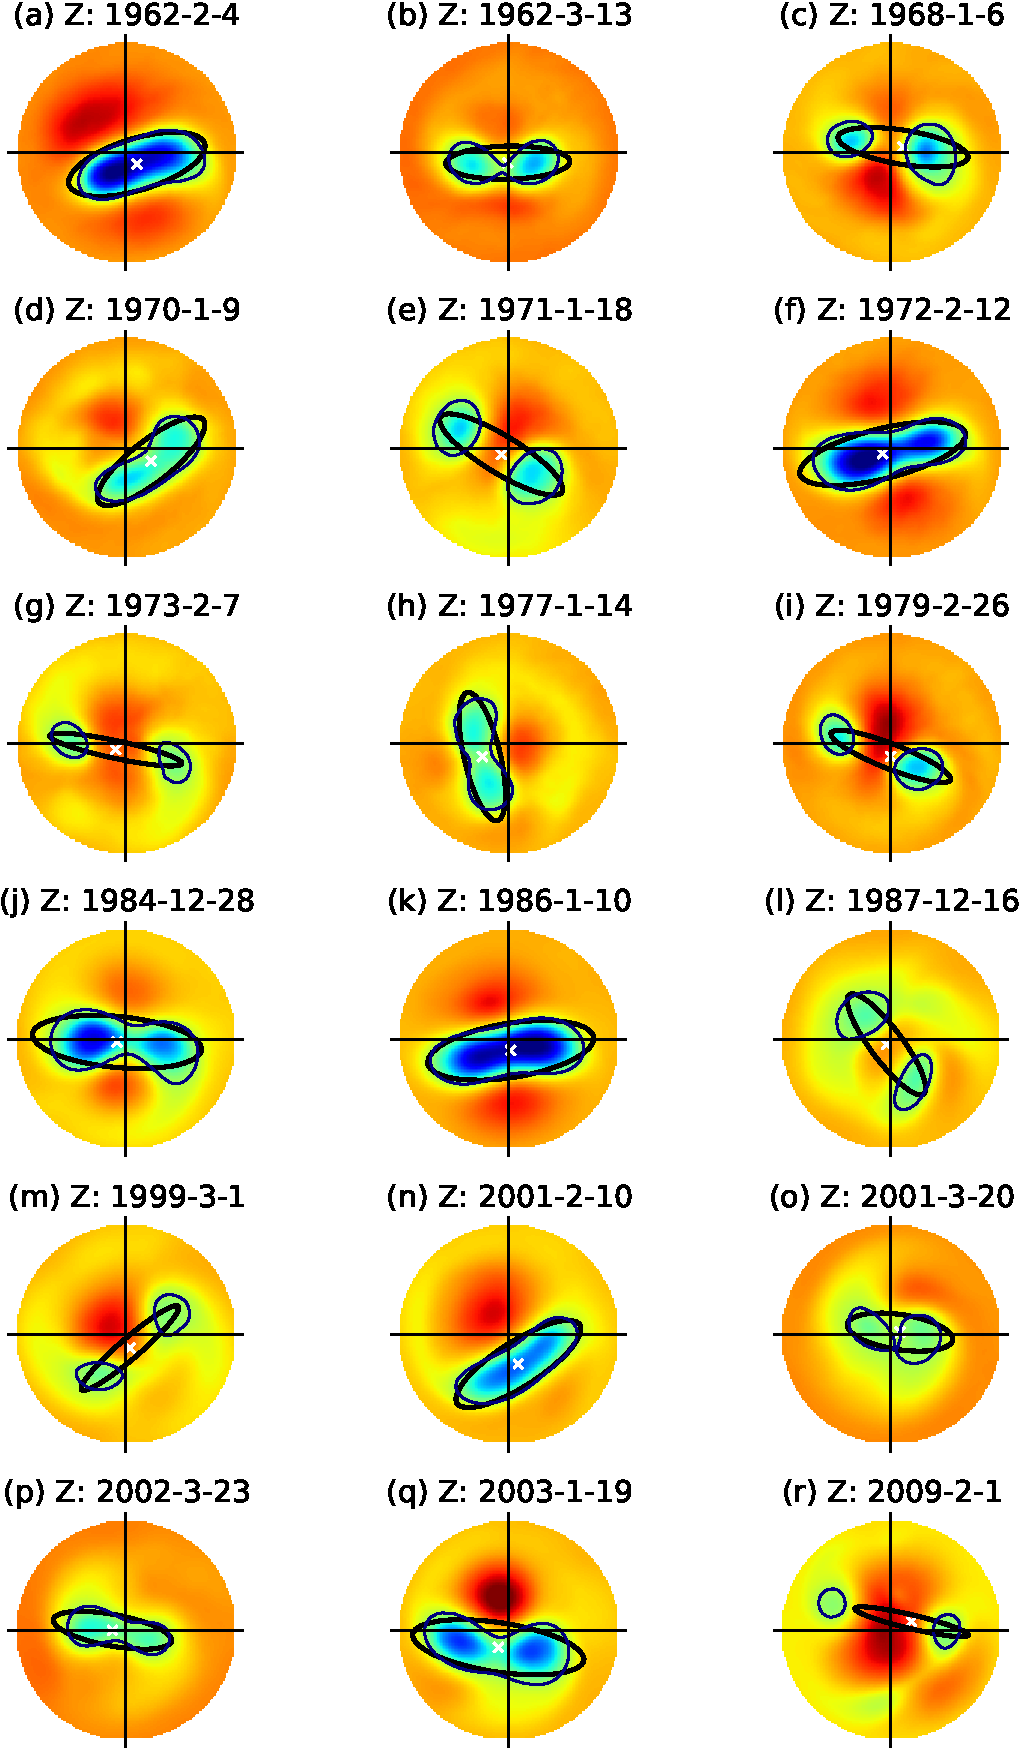
\includegraphics[width=0.8\textwidth]{figures/chapter-moments/GPH_all_events_splits.pdf}
 \caption[Geopotential height at the peak of split vortex events.]{10~hPa
   geopotential height at the peak of each of the 18 split vortex events
   identified in ERA. The peak is defined as the day with the largest aspect
   ratio during the two weeks following the onset date. The vortex edge is shown
   as a thin black contour, the equivalent ellipse the thick black contour and
   its centroid as a white cross. Data are transformed to Cartesian coordinates
   with a polar stereographic projection.}
 \label{fig:gph_all_events_splits}
\end{figure}

\begin{figure}[htbp]
 \centering
 \noindent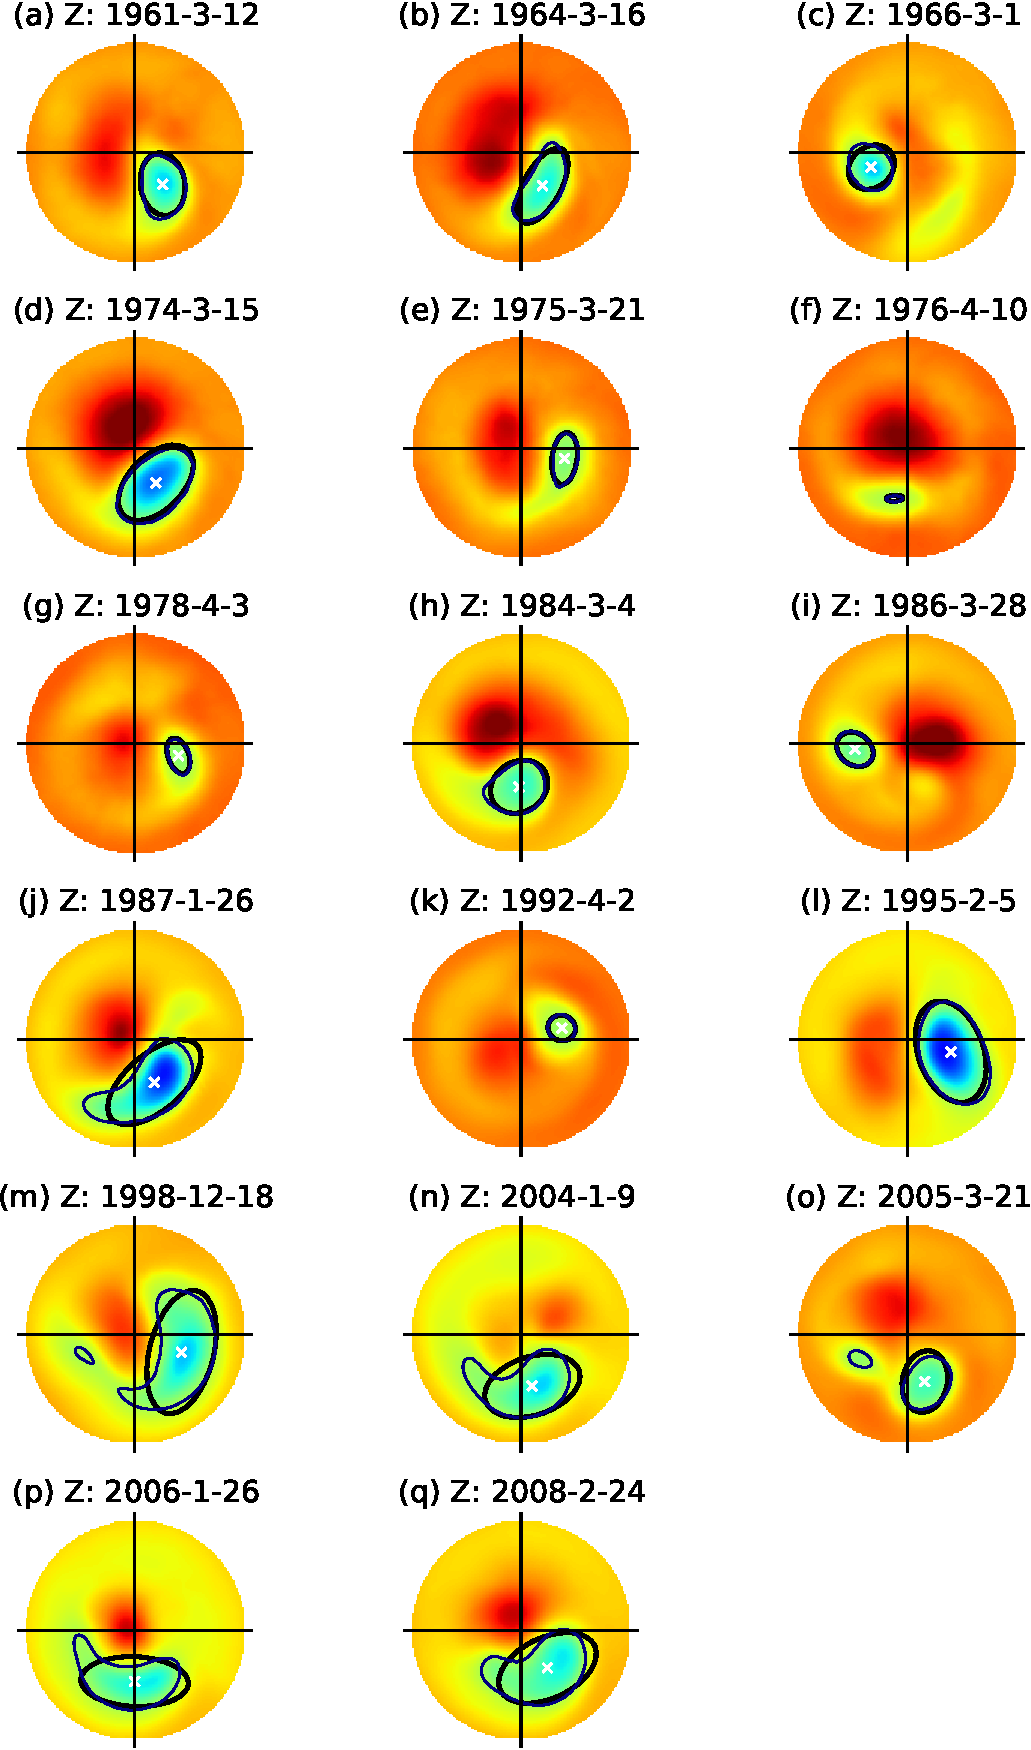
\includegraphics[width=0.8\textwidth]{figures/chapter-moments/GPH_all_events_displs.pdf}
 \caption[Geopotential height at the peak of displaced vortex events.]{As Figure
   \ref{fig:gph_all_events_splits} but for the 17 displaced vortex events
   identified in ERA.}
 \label{fig:gph_all_events_displs}
\end{figure}

Figures \ref{fig:gph_all_events_splits} and \ref{fig:gph_all_events_displs} show
geopotential height at the peak of each of the split and displaced vortex
events. The peak is defined as the day with the maximum aspect ratio or minimum
centroid latitude in the two weeks following the onset date of split and
displaced vortex events respectively. Almost all of the split vortex events show
two clearly separated vortices or a pinched vortex shape, which is approximately
symmetrical about the North Pole. Two exceptions are Figures
\ref{fig:gph_all_events_splits}(a) and (k), in which the vortex is highly
elliptical but not clearly split. Figure \ref{fig:gph_all_events_splits}(n)
shows an event with a highly elliptical vortex that is also somewhat displaced
from the pole, indicating that it has some displaced nature. The majority of
split vortex events are seen to occur along the $90^{\circ}$E-$90^{\circ}$W
axis, in line with the climatological wave-2 pattern \citep{Andrews1987}. Figure
\ref{fig:gph_all_events_splits}(h) shows an exception to this, with an
orientation orthogonal to the majority of events.

The displacement events mostly show a smaller and weaker vortex, owing to the
fact that they are more common later in winter (see Figure
\ref{fig:z_m13_cp07_histogram}). Some events, particularly those occurring in
late March, are also likely to be events which would traditionally be defined as
final warmings. It can be seem that the majority of displacement events occur in
the direction of the 0-90$^{\circ}$E quadrant, again in line with the
climatological wave-1 pattern. However, there are some exceptions to this, for
instance Figures \ref{fig:gph_all_events_displs} (c) and (i), which  show a
westward-displaced vortex. 



\subsection{Comparison with CP07 and M13}

\begin{table}
  \begin{centering}
    \begin{tabular}{llcrr}  \hline
    No. & Event onset & Event type & $\Delta \mathrm{T}_{10}$~(K) &
                                                                    $\overline{u}_{10}~(\mathrm{m~s^{-1}})$ \\ \hline
    1*  & 1961-3-9    & D          & 10.2       & 2.7 \\
    2*  & 1962-1-30   & S          & 1.9        & 38.9 \\
    3*  & 1962-3-7    & S          & -1.0       & 16.9 \\
    4*  & 1964-3-15   & D          & 11.9       & 1.3 \\
    5$\dagger$  & 1966-2-26   & D          & 2.5        & -5.9 \\
    6   & 1967-12-29  & S          & 13.0       & 19.4 \\
    7$\dagger$   & 1970-1-5    & S          & 8.5        & -4.0 \\
    8   & 1971-1-15   & S          & 10.8       & -1.7 \\
    9*  & 1972-2-4    & S          & -1.6       & 33.6 \\
    10$\dagger$  & 1973-2-4    & S          & 7.3        & -6.6 \\
    11* & 1974-3-12   & D          & 5.3        & -4.8 \\
    12* & 1975-3-16   & D          & 7.6        & -8.0 \\
    13* & 1976-3-31   & D          & 8.2        & -13.3 \\
    14$\dagger$  & 1977-1-7    & S          & 7.6        & -5.5 \\
    15*$\dagger$ & 1978-3-25   & D          & 2.5        & -9.3 \\
    16  & 1979-2-18   & S          & 5.6        & -0.4 \\
    17  & 1984-2-25   & D          & 11.6       & -4.4 \\
    18  & 1984-12-25  & S          & 15.0       & -1.7 \\
    19* & 1986-1-7    & S          & 3.4        & 29.9 \\
    20* & 1986-3-21   & D          & 9.1        & -12.2 \\
    21  & 1987-1-20   & D          & 8.3        & -7.7 \\
    22  & 1987-12-10  & S          & 9.8        & -3.0 \\
    23* & 1992-3-22   & D          & 7.6        & -4.4 \\
    24*$\dagger$ & 1995-2-2    & D          & 5.6        & 7.7 \\
    25  & 1998-12-15  & D          & 8.2        & 8.1 \\
    26  & 1999-2-24   & S          & 6.6        & -12.7 \\
    27  & 2001-2-7    & S          & 5.2        & -7.2 \\
    28* & 2001-3-15   & S          & -6.8       & 12.1 \\
    29* & 2002-3-21   & S          & -1.5       & 5.1 \\
    30  & 2003-1-17   & S          & 6.1        & 16.8 \\
    31  & 2004-1-2    & D          & 5.8        & -4.8 \\
    32* & 2005-3-11   & D          & 3.1        & -5.0 \\
    33  & 2006-1-17   & D          & 4.2        & -14.3 \\
    34  & 2008-2-18   & D          & 4.6        & 2.3 \\
    35  & 2009-1-18   & S          & 13.2       & 16.9 \\ \hline
    \end{tabular}
    \caption{A summary table of displaced (D) and split (S) vortex events,
      identified from 10~hPa geopotential height data from 1958--2009.
      $\Delta \mathrm{T}_{10}$ represents the mean area-weighted
      $50^{\circ}$-$90^{\circ}$N cap temperature anomaly at 10 hPa calculated 5
      days either side of the event onset date. $\overline{u}_{10}$ represents
      $\overline{u}$ at $60^{\circ}$N and 10~hPa averaged over the same
      period. Asterisks (*) represent those numbers that do not coincide
      (i.e. within 10 days and of the same type) with events defined by CP07 and
      daggers ($\dagger$) events which do not coincide with events of M13.}
  \end{centering}
  \label{tab:events}
\end{table}

The split and displaced vortex events identified using the above method are now
compared with those of the CP07 and M13 methods. Table 3.1 identifies those
events which do not coincide with the events of CP07 and M13, where `coincide'
indicates events within 10 days and of the same type. Of the 35 events
identified, 16 were found not to coincide with events of CP07 (10 displacement
and 6 split). Six events were found not to coincide with those of M13 (3
displacement and 3 split), although this comparison only covers the 28 events
from 1958-2002, as it was not possible to reproduce the M13 method over the
longer period studied here because of the difficulties with hierarchical
clustering discussed in Section \ref{sec:event-definition}. Just two completely
new events were identified (i.e. not coinciding with either CP07 or M13); these
are the displaced vortex events with onset dates 1978-3-25 and 1995-2-2.

Table 3.1 also shows polar cap averaged 10~hPa temperature anomalies
($\Delta \mathrm{T}_{10}$), averaged 5 days either side of the event to give a
measure of the event magnitude. The events of CP07 show a larger average anomaly
than events identified with the current method, although the two are not
statistically significantly different: CP07 average 8.6~K [6.1, 10.9] split and
7.8~K [5.5, 9.9] for displaced vortex events, while the current method averages
5.7~K [3.0, 8.3] for split and 6.8~K [5.5, 8.2] for displaced vortex events
(numbers in square brackets represent the 95\% uncertainty range, calculated
using a bootstrap test). It can be seen that while the vast majority of events
show positive values of $\Delta \mathrm{T}_{10}$ (i.e. warming), four events
show negative values. All of these events are also identified by M13, and they
attributed the negative values to the presence of a strong, cold vortex prior to
the event. Zonal-mean zonal wind at $60^{\circ}$N and 10~hPa
($\overline{u}_{10}$), averaged over the same period is also shown in Table
3.1. The majority of events show negative values, in line with the traditional
wind reversal criterion, although some show positive values. Again this results
from a strong vortex prior to these events, as well as the fact that the new
method detects some events with a distorted but strong vortex (seen in Figures
\ref{fig:gph_all_events_splits} and \ref{fig:gph_all_events_displs}).

% Mean values 
% -----------
% DT: Split: 5.7 pm 5.7 (3.0, 8.3)
%     Displ: 6.8 pm 2.9 (5.5, 8.2)
%     Split (CP07): 8.6 pm 4.6 (6.1, 10.9)
%     Displ (CP07): 7.8 pm 3.9 (5.5, 9.9)


The seasonal distribution of split and displaced vortex events identified by the
current method ($Z_{10}$), M13, and CP07, is shown in Figure
\ref{fig:z_m13_cp07_histogram}. In all three methods split vortex events are
more frequent in early-mid winter, with a peak in January. For displaced vortex
events, both the current method and M13 show a skew towards events occurring
later in winter. However, there is less similarity with the CP07 distribution of
displaced vortex events. CP07 indicates an approximately flat distribution
throughout winter, and many fewer displaced vortex events overall. It should be
noted that the seasonal distribution of split vortex events from the moment
based methods does not arise from the underlying climatology of aspect ratio,
which remains approximately constant throughout winter (e.g., Figure
\ref{fig:cmip5_moments_stats_seas}). The centroid latitude does however, show a
small equatorwards trend throughout winter, which may to some extent account for
the seasonal distribution of displaced vortex events \citep{Mitchell2011}.

\begin{figure}
  \centering
  \noindent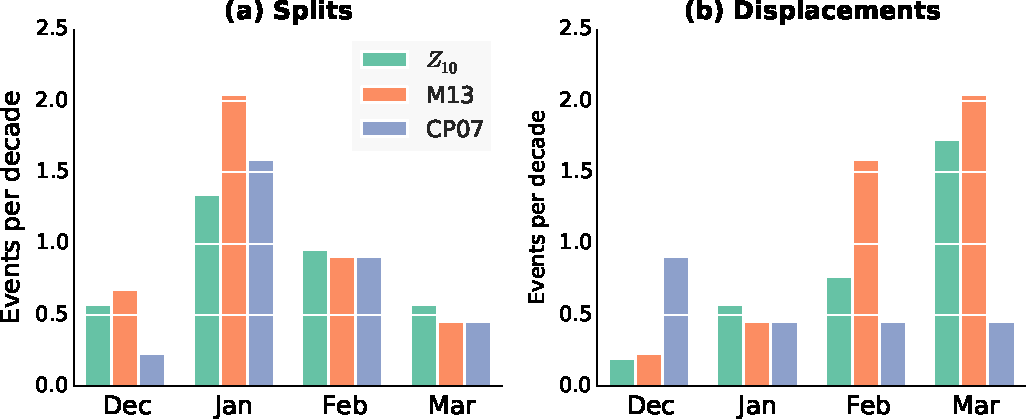
\includegraphics[width=\textwidth]{figures/chapter-moments/splits_displacements_histogram.pdf}
  \caption[Seasonal distribution of displaced and split vortex
  events.]{Histogram of the seasonal distribution of displaced and split vortex
    events, from the new geopotential height-based method ($Z_{10}$), M13 and
    CP07.}
  \label{fig:z_m13_cp07_histogram}
\end{figure}

\begin{figure}
 \centering
 \noindent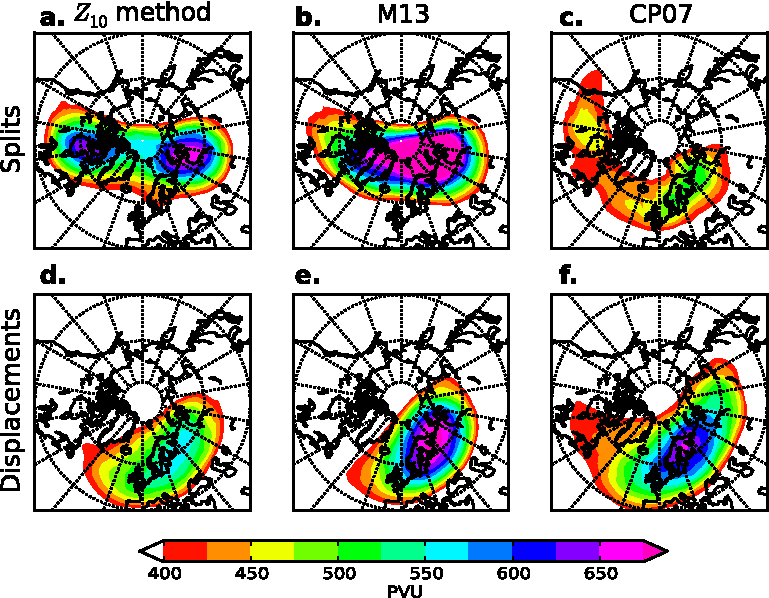
\includegraphics[width=\textwidth]{figures/chapter-moments/pv_composites_colbar_crop.pdf}
 \caption[PV composites for split and displaced vortex events.]{Composites of
   potential vorticity at the 850~K isentropic surface from the ERA reanalysis
   over 1958--2009. Composites are taken over the 5 days following the onset date
   of split vortex events (a,b,c) and displaced vortex events (d,e,f). The
   new ($Z_{10}$) method (a,b) is compared with that of M13 (b,e) and CP07
   (c,f).}
 \label{fig:pv_composites_m13_cp07}
\end{figure}

Figure \ref{fig:pv_composites_m13_cp07} compares the average shape of the
stratospheric polar vortex following the split and displaced vortex events
identified by the three methods. Composites of PV in the mid-stratosphere
(850~K) are shown averaged 5 days following each event. For the split vortex
events, the new method ($Z_{10}$) method clearly shows two separated
vortices, one centred over Canada and the other over Siberia. For the M13 events
the split vortex composite shows the vortex stretched across the same
$90^{\circ}$W-$90^{\circ}$E line, although not as clearly split, while the
composite for the CP07 events looks very different. This has a weak vortex
centred over Canada, with the other over Northern Europe in a similar location
to the composite for displaced events. All three composites for displaced events
show a vortex centred over Northern Europe, but this extends most westward in
the CP07 composite, suggesting that there may be some contamination from
misdiagnosed split vortex events.

Overall, Figure \ref{fig:pv_composites_m13_cp07} demonstrates that the new
method succeeds (in a composite sense) in identifying displaced and split vortex
events at least as well as the methods of M13 or CP07. When comparing the three
methods, CP07 is the clear outlier. This is most likely because the CP07
approach employs a zonal-mean threshold which cannot accurately capture some
extreme events (as discussed in M13).


\subsection{Comparison with zonal wave amplitudes}
\label{sec:comp-zonal-wave}

Many studies have characterised stratospheric polar variability by its zonal
wave structure \citep[e.g,][]{Randel1988,Yoden1999,Nakagawa2006,Bancala2012}. It
is therefore instructive to compare this wave analysis with the moment
diagnostics developed above. Here this is carried out for the displaced and
split vortex events shown in Figures \ref{fig:displaced_ellipse} and
\ref{fig:split_ellipse} respectively. A similar comparison was shown by
\citet{Waugh1997} and \citet{Waugh1999}, and the results here are consistent
with their findings.

Zonal wavenumber decomposition is carried out by taking the Fourier transform of
the 60$^{\circ}$N, 10~hPa geopotential height field over all longitudes. The
amplitude of wave-$n$ on a given day is then given by the modulus of the $n$th
Fourier component on that day. In ERA data, the amplitude of DJFM wave-2 is, on
average, about 30\% that of wave-1, and wave-3 13\% of wave-1, indicating a
Charney-Drazin filtering of zonal wavenumbers, as discussed in Section
\ref{sec:planetary-waves}.

The correlation of geopotential height-derived daily aspect ratio and the wave-2
amplitude over DJFM is 0.30 and that of centroid latitude and wave-1 amplitude
$-0.22$, both of which are highly statistically significant. Figure
\ref{fig:wave_moments_ts} illustrates these relationships for the example split
and displaced vortex events previously shown in Figures
\ref{fig:displaced_ellipse} and \ref{fig:split_ellipse} . In the case of the
1979 split vortex event the wave-2 amplitude peaks approximately 5 days before
the peak of the aspect ratio. Wave-2 amplitude is also more variable than aspect
ratio in early winter, although the two are correlated at this time. In the case
of the 2006 displaced vortex event, the difference is even greater. The wave-1
amplitude peaks about three weeks before the centroid latitude, and is actually
anomalously small at the peak of centroid latitude. Before and after the event,
the wave-1 amplitude and centroid latitude are highly correlated.

A result of these differences is that not all split vortex events are defined as
wave-2 warmings and not all displaced vortex events as wave-1 warmings. For
example, the split vortex events with onset dates 1973-2-7, 1987-12-10, and
1999-2-24 are classified as wave-1 warmings by \citet{Bancala2012}. However, the
structure of the vortex appears clearly split in these three examples (see
Figures \ref{fig:gph_all_events_splits} (g), (l) and (m)), highlighting the
differences in these classifications.

The physical reasons for these differences are investigated in Figure
\ref{fig:wave_moments_vortex}. This compares the vortex structure at the peak
wave amplitude and peak aspect ratio/centroid latitude for the two events. For
the 1979 split vortex event, the vortex appears split at both times but there is
a greater separation between the vortices at the time of maximum aspect
ratio. The wave-2 amplitude is greatest at the earlier time, however, because
the vortices (particularly the eastern vortex) are stronger. Similarly for the
2006 event, at the time of maximum wave-1 amplitude the vortex is not displaced
far from its average position but its strength means that the wave-1 amplitude
is greater than the much more displaced vortex found later. Generally, the
sensitivity of wave amplitudes to vortex strength means that wave amplitudes may
actually decline during periods of intense wave breaking due to the weakening of
the vortex, even if that vortex is significantly distorted.

Overall, these results show that as the vortex departs from zonal symmetry
linear wave theory breaks down and changes in the wave-1 and wave-2 amplitudes
cannot be simply interpreted as changes in the position and elongation of the
vortex respectively.


\begin{figure}
 \centering
 \noindent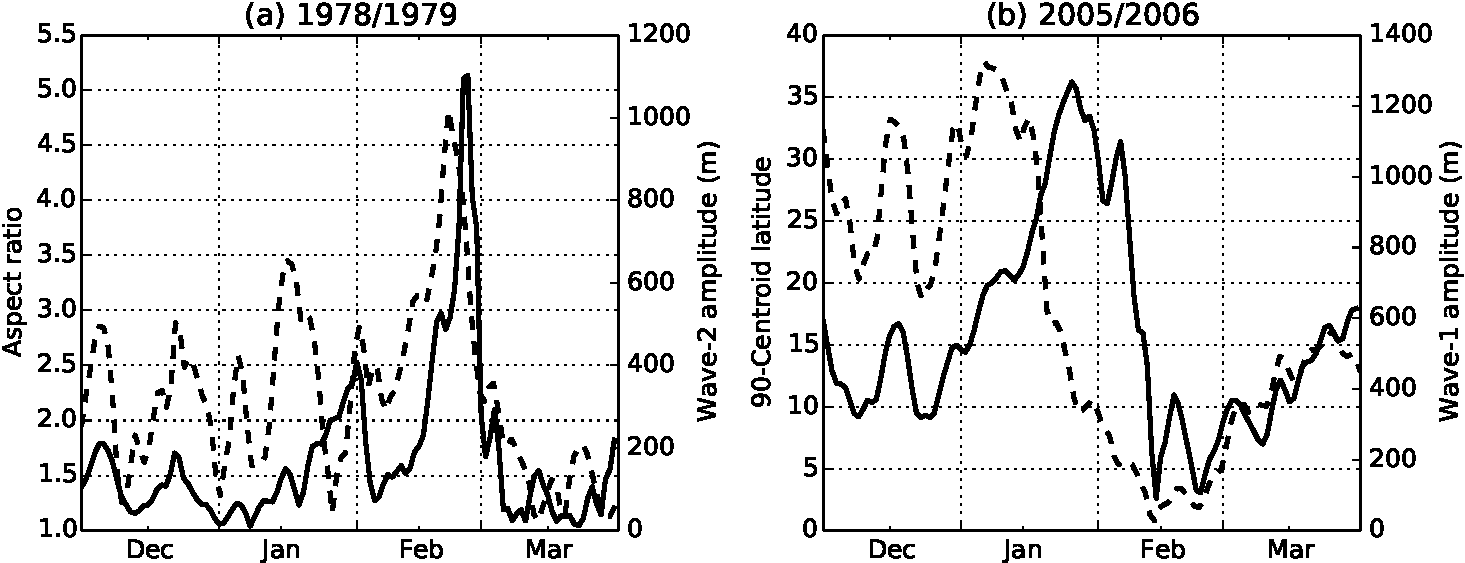
\includegraphics[width=\textwidth]{figures/chapter-moments/waves_moments_ts.pdf}
 \caption[Wave amplitude and moment diagnostic time series.]{(a) Aspect ratio
   (solid line) and wave-2 amplitude (dashed line) over the winter
   1978-1979. (b) Centroid latitude (solid line) and wave-1 amplitude (dashed
   line) over the winter 2005-2006. Centroid latitude is expressed as its
   deviation from the North Pole.}
 \label{fig:wave_moments_ts}
\end{figure}

\begin{figure}
 \centering
 \noindent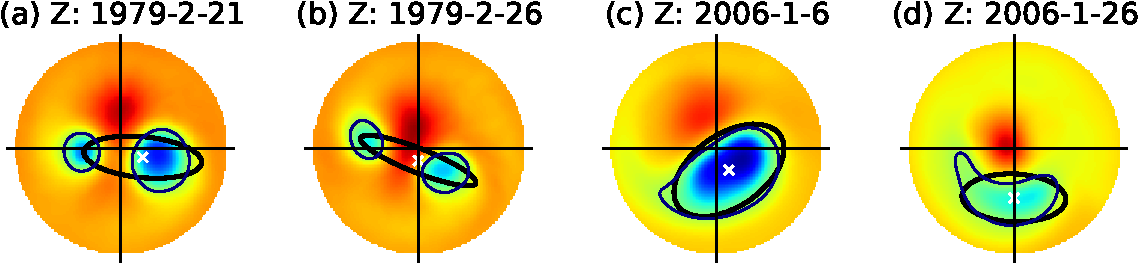
\includegraphics[width=\textwidth]{figures/chapter-moments/wave_moment_vortices.pdf}
 \caption[Vortices at maximum of moment diagnostics and wave amplitudes.]{10~hPa
   geopotential height on the day of maximum wave-2 amplitude (a) and maximum
   aspect ratio (b) for the 1979 split vortex event; and maximum wave-1
   amplitude (c) and minimum centroid latitude (d) for the 2006 displaced vortex
   event. The vortex edge contour, equivalent ellipse, and centroid latitude are
   shown as Figure \ref{fig:displaced_ellipse}.}
 \label{fig:wave_moments_vortex}
\end{figure}


\section{Stratosphere-troposphere coupling}
\label{sec:moments_analysis}

\subsection{Tropospheric response}

Having verified that this new method identifies split and displaced vortex
events as skillfully as previous methods, it is now possible to study their
influence on the troposphere. This is motivated by the result of M13 who, as
discussed in Section \ref{sec:observ-evid}, found tropospheric anomalies to be
larger following split vortex events that displaced vortex events. Figure
\ref{fig:dripping_paint}(a,b) shows time-height composites of the NAM over the
90 days following split and displaced vortex events. Here the method of
\citet{Baldwin2009} is used to define the NAM as the leading empirical
orthogonal function (EOF) of daily wintertime (November-April) zonal mean
geopotential height anomalies poleward of $20^{\circ}$N. The anomalies are
calculated by subtracting the seasonal cycle which has been smoothed with a
90-day low-pass filter. The daily NAM anomalies are then determined by
projecting daily geopotential anomalies onto the leading EOF patterns. Finally,
the NAM is normalised so that the time series at each level has unit variance.

\begin{figure}
 \centering
 \noindent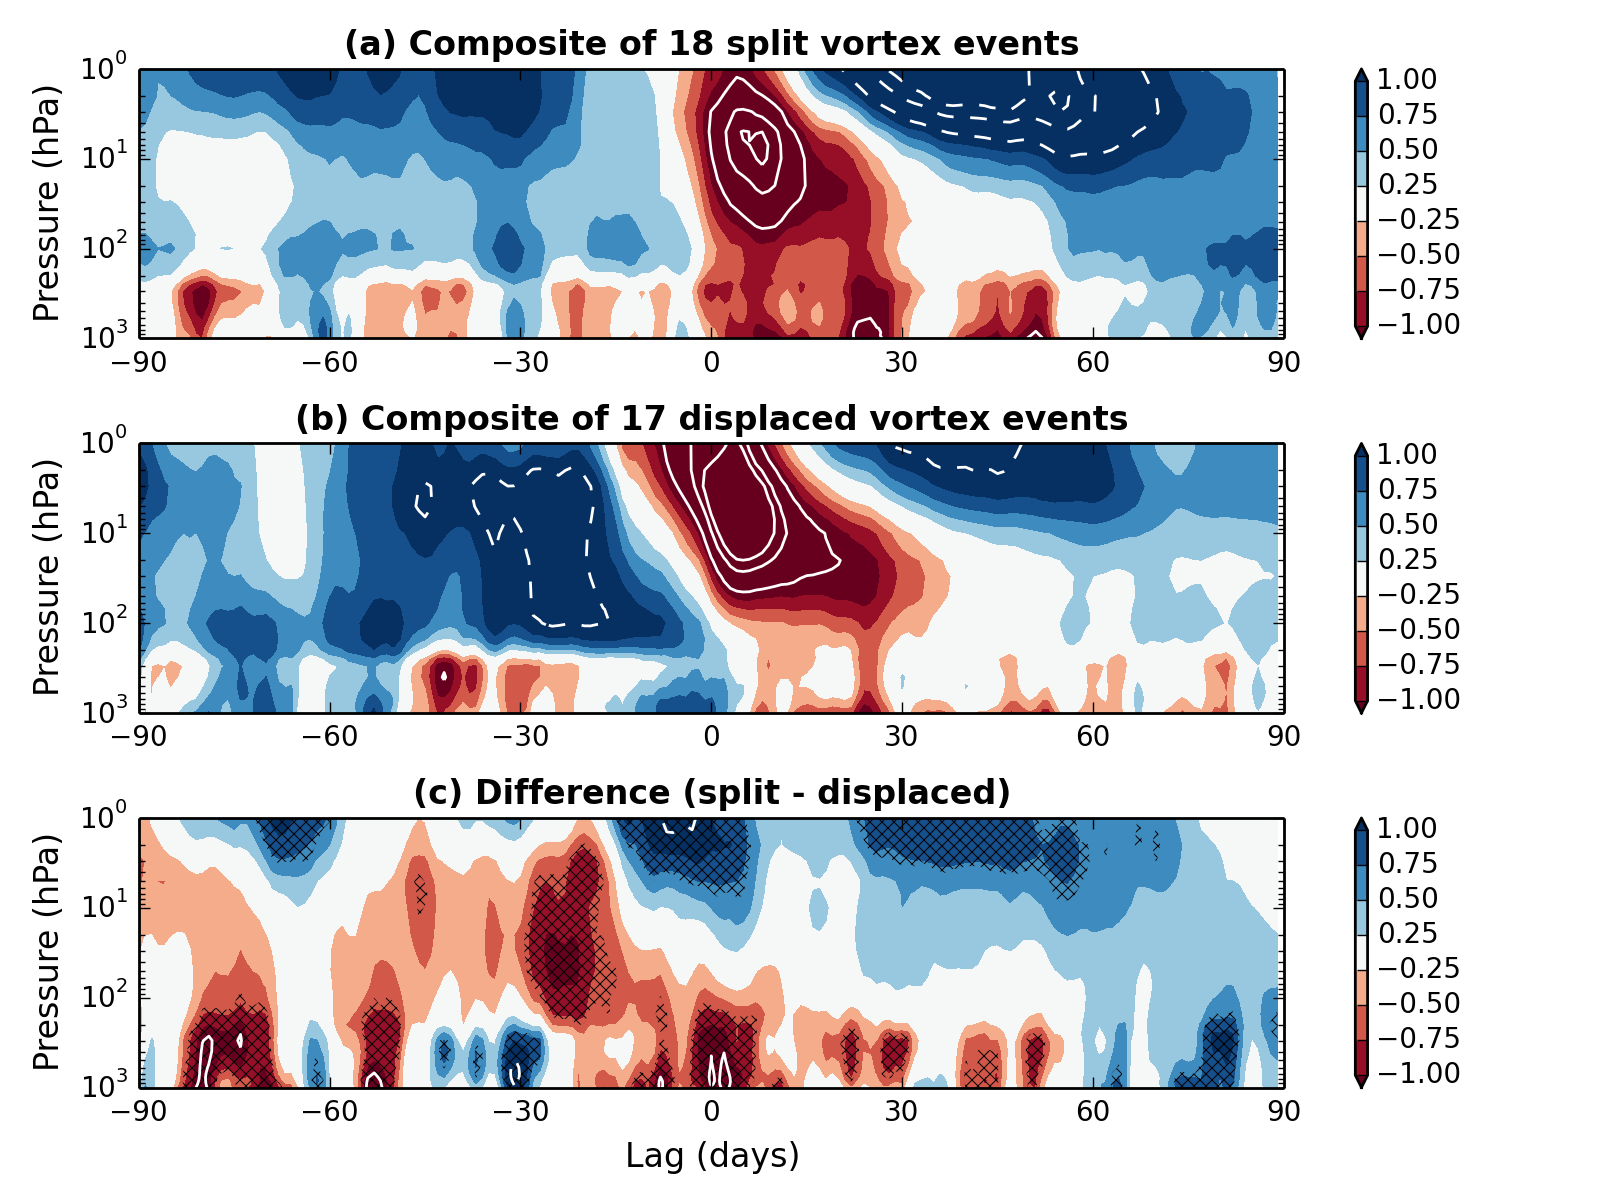
\includegraphics[width=\textwidth]{figures/chapter-moments/dripping_paint.png}
 \caption[NAM composites for split and displaced vortex events.]{Composites of
   the time-height evolution of the NAM during (a) 17 vortex displacement events
   and (b) 18 splitting events. (c) shows the difference in these composites,
   and hashed regions represent those that are 95\% significant according to a
   two-tailed bootstrap test. Lag 0 is at the onset of an event as measured at
   10 hPa. Contour intervals are 0.25 and the region between -0.25 and 0.25 is
   unshaded. Data is from the ECMWF Reanalyses 1958--2009.}
 \label{fig:dripping_paint}
\end{figure}


In agreement with M13, it can be seen that the tropospheric NAM is more negative
during the 60 days following split vortex events than displaced vortex
events. Also similar to M13 is the fact the vertical evolution for the two
events greatly differs, with split vortex events occurring almost
instantaneously throughout the depth of the atmosphere and displaced vortex
taking almost two weeks to propagate through the stratosphere. The
near-barotropic nature of split vortex events suggests that resonant excitation
of the barotropic normal mode \citep{Esler2005} may be an important influence in
this case.
% Furthermore, the rapid onset of split vortex events is ... (Love 1893).

The difference in the NAM composites (split minus displaced) is shown in Figure
\ref{fig:dripping_paint}(c). Statistical significance of this difference is
calculated with the null hypothesis that there is no difference between the NAM
response to split and displaced vortex events, and assessed using a two tailed
bootstrap test with the following procedure:
\begin{enumerate}[i.]
\item The labels `split' and `displacement' are randomly re-assigned to the 35
  events.
\item NAM composites and the composite difference of these randomly assigned events
  are calculated. 
\item The above steps are repeated $10~000$ times, to form a distribution
  of random composite differences. If the true composite difference lies
  $<2.5\%$ or $>97.5\%$ within this distribution, then it can be said to be 95\%
  significant.
\end{enumerate}
Some significant differences are seen between the split and displaced vortex
composites. For instance, a more positive stratospheric NAM is seen to precede
displaced vortex events, while the dipole in the upper stratospheric and
tropospheric NAM near lag 0 represents the difference in baroclinicity of the
two types of event. Some regions of significant differences are seen in the
tropospheric NAM 0-60 days after the event, but there are also some regions that
are not significant. Care must be taken when interpreting the importance of
small significant regions these may arise by chance, even if no physical
relationship exists.

\begin{figure}
 \centering
 \noindent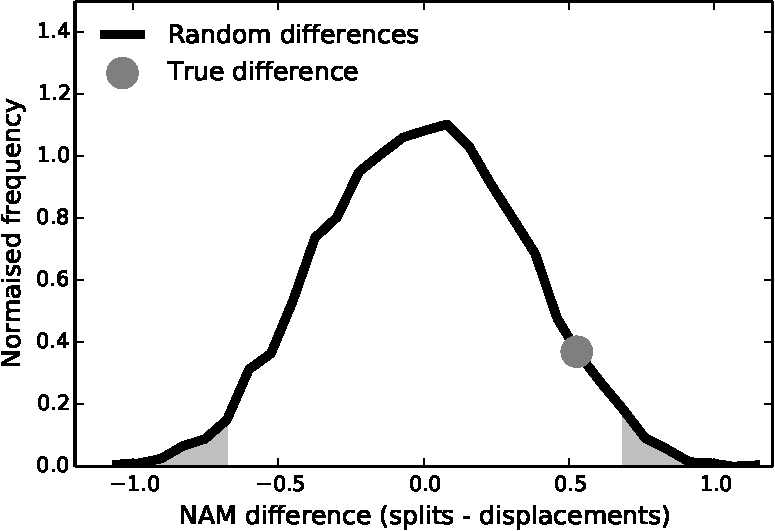
\includegraphics[width=0.6\textwidth]{figures/chapter-moments/nam_difference_sig.pdf}
 \caption[Significance test of surface NAM difference]{Distribution of 0-30 day
   mean surface NAM composite differences between split and displaced vortex
   events, formed by randomly shuffling the labels `split' and `displacement'
   between events. The 95\% significant region (according to a two-tailed test;
   i.e. $<2.5$\% and $>97.5$\%) is shaded and the true composite difference is
   at the 94th percentile.}
 \label{fig:nam_comp_diff}
\end{figure}

The difference in the tropospheric anomalies following split and displaced
vortex events can be tested more robustly by examining surface anomalies
averaged over the 30 days following onset. This difference is again tested using
the bootstrap procedure outlined above. The distribution of randomly calculated
surface NAM composite differences, and the actual surface NAM composite
difference are shown in Figure \ref{fig:nam_comp_diff}. It can be seen that the
true NAM difference does not lie in the 95\% significant region, so the null
hypothesis that there is no difference between surface NAM anomalies following
split and displaced vortex events cannot be rejected. It should be noted that
the statistical test here is different to that carried out by M13. They tested
whether the surface NAM following split and displaced vortex events were
different from randomly selected winter dates, finding that anomalies following
splits are, but those following displacements are not. They did not, however,
test the \emph{difference} between split and displaced vortex events.

\begin{figure}
 \centering
 \noindent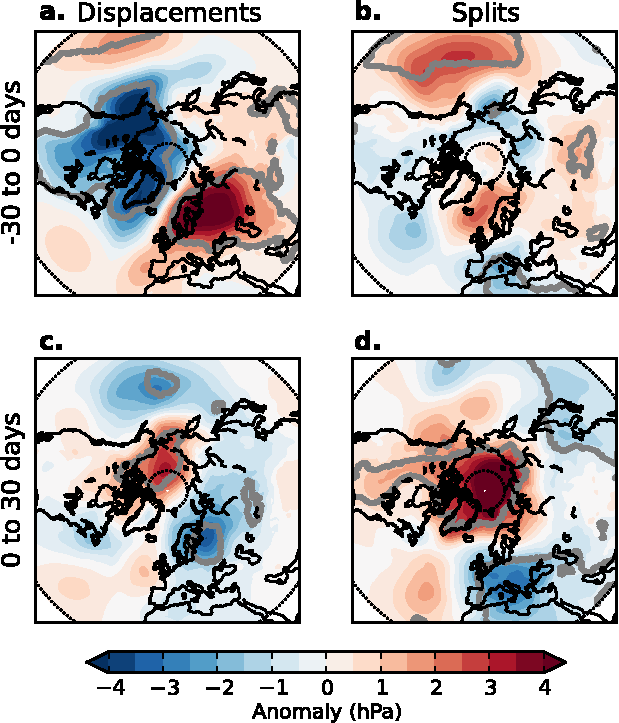
\includegraphics[width=0.7\textwidth]{figures/chapter-moments/mslp_composites_colbar_crop.pdf}
 \caption[Mean sea-level pressure composites for split and displaced vortex
 events.]{Composites of mean sea-level pressure anomalies in the 30 days before
   (a,b) and 30 days after (c,d) the onset dates of displaced (a,c) and split
   (b,d) vortex events from the $Z_{10}$ method. Data are from the ECMWF
   renalyses (1958--2009). Anomalies are calculated for each day and gridpoint
   from the climatology for that day of the year and gridpoint. Grey contours
   indicate regions of greater than 95\% statistical significance according to a
   bootstrap significance test.}
 \label{fig:mslp_composites}
\end{figure}

The surface NAM does not provide the full description of surface variability,
and so in Figure \ref{fig:mslp_composites} composites of MSLP 30 days before and
30 days following the onset dates of displaced and split vortex events are
presented. Statistical significance is calculated against the null hypothesis
that anomalies before and after split and displaced vortex events are
indistinguishable from other winter dates. This is again estimated from a
two-tailed bootstrap test, in which $10~000$ composites of equal size are formed
from randomly selected winter dates, and the percentile of the true composite
calculated from this distribution.

The strongest precursor is found for displaced vortex events, with a wave-1
pattern that is similar to the climatological stationary wave pattern
\citep[e.g.,][]{Garfinkel2008}, suggesting increased wave-1 propagation into the
stratosphere. However, the strongest anomalies following events occur after
split vortex events, with a pattern resembling the negative phase of the NAM,
though with a southern centre of action shifted towards Europe. A further
difference between the split and displaced vortex composites is that there is a
more negative MSLP anomaly over Scandinavia and Siberia following displaced
vortex event. Overall, the main features of Figure \ref{fig:mslp_composites}
compare very well with the corresponding diagnostics from M13.



\subsection{Tropopause response}

\begin{figure}
 \centering
 \noindent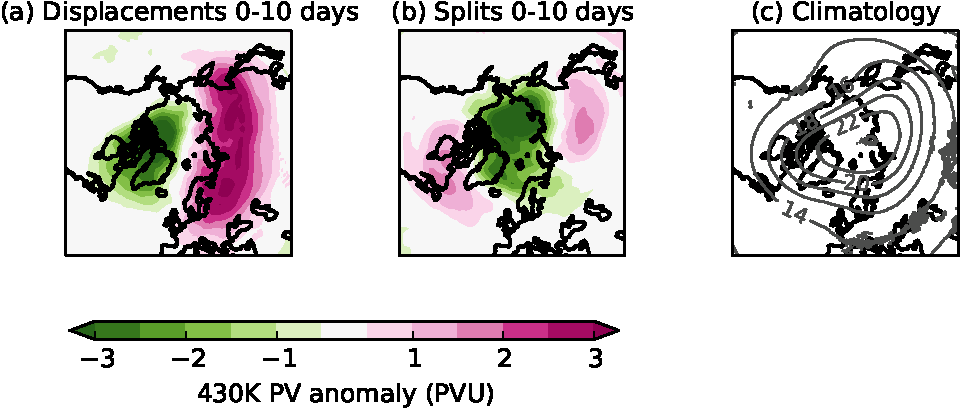
\includegraphics[width=\textwidth]{figures/chapter-moments/PV_430K.pdf}
 \caption[Composites of 430~K PV]{Composite of PV anomalies on the 430~K
   isentropic surface averaged over the 10 days following displaced (a) and
   split (b) vortex events. DJFM average of 430~K PV (c). Units are PVU and the
   contour interval is 2~PVU. Data are restricted to the ERA-Interim period
   (1979--2009), meaning a total of 10 displaced and 10 split vortex events enter
   the composites. }
 \label{fig:430K_PV}
\end{figure}
 

\begin{figure}
 \centering
 \noindent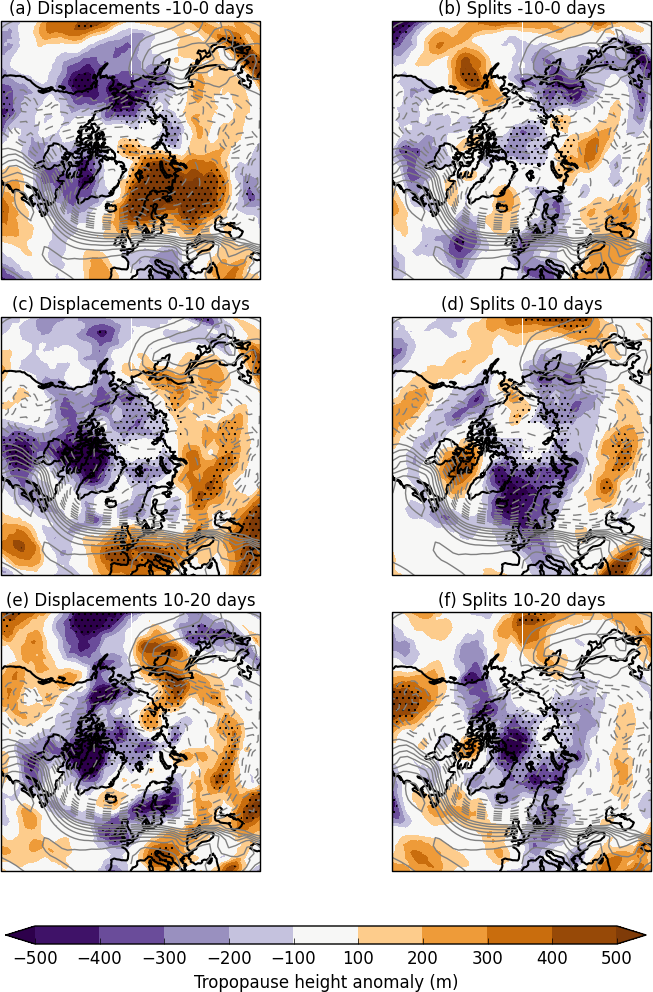
\includegraphics[width=0.8\textwidth]{figures/chapter-moments/tropopause_height_composites_nam_crop.png}
 \caption[Tropopause height composites for split and displaced vortex
 events.]{Composites of tropopause height anomalies averaged 10 days before
   (a,b), 10 days after (c,d) and 10-20 days after displaced and split vortex
   events (filled contours). Anomalies are calculated for each day and gridpoint
   from the climatology for that day of the year and gridpoint. Stippling
   indicates regions of greater than 95\% statistical significance according to
   a Monte-Carlo significance test. Grey contours indicate the first EOF of NH
   mean sea-level pressure, which explains 33\% of the variance (dashes
   represent negative values).}
 \label{fig:tropopause_height}
\end{figure}

The mechanism of the stratosphere's influence on the troposphere proposed by
\citet{Ambaum2002} states that changes in the PV near the tropopause affect the
tropopause height and induce tropospheric anomalies below (more details are
given in Section \ref{sec:mechanisms}). In order to investigate this mechanism,
composites of PV anomalies at the 430~K isentropic surface (which lies close to
100~hPa; just above the tropopause), over the 10 days following displaced and
split vortex events are shown in Figures \ref{fig:430K_PV}(a,b). Data at this
isentropic level were not available for ERA-40 so these composites are limited
to the ERA-Interim (1979-2009) period, meaning 10 events of each type enter the
composites. The shorter 10-day period was chosen to reflect the typical time
scale for the split or displacement of the vortex, rather than the longer time
scale taken for the re-formation of the vortex. However, composites taken over
30 days, as in Figure \ref{fig:mslp_composites}, show similar structure but with
reduced magnitude (similarly, composites taken over 5 days, as in Figure
\ref{fig:pv_composites_m13_cp07}, show slightly increased magnitude). In the
displaced composite case a region of high PV is seen over Siberia and
Scandinavia, consistent with the movement of the vortex over this region. Note
that this is shifted further east than the position of the vortex at 850~K
($\sim 10$~hPa) (Figure \ref{fig:pv_composites_m13_cp07}(d)), again indicating
the more baroclinic nature of displaced vortex events (this westward tilt with
height was also found by \citet{Matthewman2009}). The split vortex composite
shows two regions of raised PV which are approximately co-located with the two
vortices at 850~K.

Again following the reasoning of \citet{Ambaum2002}, composites of tropopause
height averaged over the 10 days before, 0-10 days after, and 10-20 days after
split and displaced vortex events are now shown in Figure
\ref{fig:tropopause_height} (these composites now use the full ERA (1958-2009)
data set). The measure of tropopause height used is that of \citet{Wilcox2012},
who construct a blended thermal and dynamical tropopause. Significance is again
calculated using a two-tailed bootstrap test.

In line with the MSLP anomalies shown in Figure \ref{fig:mslp_composites},
tropopause height anomalies are seen to be larger prior to displaced vortex
events, with a wave-1-like structure. Following the events, tropopause height
anomalies are seen to approximately mirror the stratospheric PV anomalies
(Figure \ref{fig:430K_PV}). That is, following displaced vortex events an
elevated tropopause is seen over Europe and Scandinavia, with a lowered
tropopause over Canada, and following split vortex events two regions of
elevated tropopause are present over Canada and Siberia with a depression in
between.

It is possible to quantitatively examine (although only approximately) whether
these tropopause anomalies are consistent with the changes in stratospheric PV
above. Changes in tropopause pressure, $\Delta p_{\mathrm{trop}}$, are related
to changes in stratospheric PV, $\Delta q$, through
\begin{equation}
\Delta q \approx -q(1+\mathrm{Bu})\frac{\Delta
  p_{\mathrm{trop}}}{p_{\mathrm{trop}}} \, , 
\label{eqn:pv_trop}
\end{equation}
where $\mathrm{Bu}$ is the Burger number, which is approximately equal to one
for any PV anomaly \citep{Ambaum2002}. The change in tropopause height,
$\Delta h_{\mathrm{trop}}$ can be calculated using the hydrostatic relation
\begin{equation}
\Delta h_{\mathrm{trop}} = -\frac{\Delta p_{\mathrm{trop}}}{p_{\mathrm{trop}}}
\frac{R T_{\mathrm{trop}}}{g} \, , 
\end{equation} 
where $T_{\mathrm{trop}}$ is the tropopause temperature. Hence
\begin{equation}
\Delta h_{\mathrm{trop}} = \frac{\Delta q}{q}
\frac{RT_{\mathrm{trop}}}{g(1+\mathrm{Bu})} \, .
\end{equation}
From Figures \ref{fig:430K_PV}(a,b) a typical 430~K PV anomaly is 2~PVU, and the
background climatology is approximately 20~PVU (Figure \ref{fig:430K_PV}(c)), so
$\Delta q/q \approx 0.1$. With a typical value of
$T_{\mathrm{trop}} = 210~\mathrm{K}$, this then gives a change of tropopause
height of $\Delta h_{\mathrm{trop}} \approx 300~\mathrm{m}$, which is indeed
approximately in line with the tropopause height anomalies seen in Figure
\ref{fig:tropopause_height}. This, along with the fact that the pattern in
tropopause height anomalies approximately mirrors that of stratospheric PV
anomalies, suggests that these tropopause height anomalies are induced by
changes in stratospheric PV above.

Also shown in Figure \ref{fig:tropopause_height} is the surface NAM pattern (the
leading EOF of DJFM daily MSLP). It can be seen that following split vortex
events more than displaced (especially days 0-10), the negative tropopause
height north of Iceland aligns more closely with the minimum in the NAM (this
region is also a node of the NAO). This may be significant if it is expected
that the fluctuation-dissipation theorem (FDT) holds in the tropospheric
response to stratospheric forcing. For systems in which the FDT holds, the
response of a system projected on a mode of variability should linearly scale
with the projection of the forcing on that mode \citep{Ring2008}. Under the
assumption that the tropopause height perturbation represents the ``forcing'',
this may project more strongly on the NAM/NAO following split vortex events,
consistent with a greater surface response to these events. Overall, however,
the pattern correlations between the split and displaced vortex tropopause
height anomalies and the NAM are not statistically significantly different
because the tropopause height field is very noisy. In order to give a more
detailed analysis a greater number of events would be needed.


\section{Conclusions}

Recent research has demonstrated the need to distinguish between split and
displaced stratospheric polar vortex events because of their different dynamics
and impacts on the troposphere. However, previous methods to identify these
events are impractical for application to climate model or seasonal prediction
simulations because they are highly sensitive to model climatology or rely on
non-standard variables. Motivated by this, we have developed a new method to
identify displaced and split vortex events which requires only geopotential
height at 10~hPa. The method is summarised as follows:
\begin{enumerate}[i.]
\item To identify the vortex region, a single contour of 10~hPa geopotential
  height is selected. This is the value of the DJFM mean zonal-mean at
  $60^{\circ}$N.
\item Using this contour the centroid latitude and aspect ratio moment
  diagnostics can be calculated.
\item Events are identified using a threshold criterion: Displaced events are
  said to occur if the centroid latitude remains equatorward $66^{\circ}$N for 7
  days or more. Split events are said to occur if the aspect ratio remains above
  2.4 for 7 days or more. In order to ensure that events are not counted twice,
  no two events may occur within 30 days.
\end{enumerate}
Results show that vortex moment diagnostics derived from geopotential height in
this way are highly correlated with those derived from PV, although fewer high
aspect ratio values are seen. The use of geopotential height here is motivated
by the fact that it is commonly output by climate models, whereas PV is
not. However, in cases where PV is available (such as in reanalyses) its use is
preferable because of its quasi-conservative properties and smaller-scale
features. The above method can be easily adapted for use with PV-based vortex
moments.

Analysis of the stratosphere following events identified by this method
demonstrates that it is able to accurately identify split and displaced vortex
events. Most of the events identified coincide with those of M13, and about
half with events identified by CP07. Composite analysis indicates that the
position of the stratospheric polar vortex following these events is at least as
extreme as that from the previous methods. 

Having identified these events, their impact on the troposphere has been
investigated. Composites of the NAM indicate a more negative surface NAM over
the month following split vortex events than following displaced vortex
events. This supports the finding of M13, using a different event identification
method and extended data set. However, using a bootstrap test the composite
\emph{difference} of the surface NAM is not found to be statistically
significant.

Anomalies of tropopause height following split and displaced vortex events are
found to be co-located with lower-stratospheric PV anomalies. They are also of a
magnitude consistent with being induced by changes in the stratospheric polar
vortex. Surface anomalies induced by changes in tropopause height may therefore
explain the different surface anomalies following split and displaced vortex
events. However, it is not possible to draw firm conclusions on this because of
the relatively small number of events and the noise of the MSLP and tropopause
height fields.

Overall, statistically significant results about the difference in the
tropospheric response to split and displaced vortex events will require a larger
number of events. This is achieved through the analysis of climate model
simulations in the next chapter.  





%%% Local Variables:
%%% mode: latex
%%% TeX-master: "thesis"
%%% End:








\chapter{Representation of vortex variability in climate models}
\label{cha:models}


\section{Introduction}
\label{sec:models_introduction}

Over the past decade an increasing number of climate models have included a
well-resolved stratosphere, with model lids above the stratopause. For example,
the fifth Coupled Model Intercomparison Project (CMIP5) \citep{Taylor2012}
includes 15 models with an uppermost level above the stratopause, whereas the
previous intercomparison project, CMIP3, includes only five
\citep{Cordero2006}. The CMIP5 model simulations are significant in that they
are evaluated in the the Intergovernmental Panel on Climate Change (IPCC) Fifth
Assessment Report (AR5) \citep{Stocker2013}. This change in model stratospheric
resolution has been largely motivated by an increased understanding of the
stratosphere's influence on tropospheric climate (discussed in
\citet{Gerber2012} and Chapters \ref{cha:introduction} and \ref{cha:moments}).

The effect of this greater stratospheric resolution was studied by
\citet{Charlton-Perez2013}, who compared stratospheric variability between
high-top and low-top models within the CMIP5 ensemble (they defined ``high-top''
as a model lid above 1~hPa, and ``low-top'' below). They found that the low-top
models have a weaker and less realistic representation of daily to interannual
polar stratospheric variability than high-top models, and attributed this to the
fact that the low-top models simulate fewer SSW events than high-top. This is
combined with a slightly weaker tropospheric NAM response in the two months
following SSW events in the low-top compared to high-top models.

These results are supported by similar studies which compared natural
variability in high and low-top versions of the same model. \citet{Cagnazzo2009}
found that a high-top model gave a more realistic representation of the
influence of ENSO on the NH extratropical stratosphere. Similarly,
\citet{Hardiman2012a} showed the influence of the QBO on the extratropics as
well as decadal trends in the NAO were more realistically simulated by the
high-top than the low-top model. These differences have again been linked to the
different simulation of SSW events in high- and low-top models
\citep{Sassi2010}.

Other studies have compared simulations of climate change with high- and low-top
models. \citet{Huebener2007} linked a increased weakening of the stratospheric
polar vortex in high-top simulations to a more southward shift of the NH winter
storm track, which in turn affects trends in North Atlantic temperatures and
precipitation. \citet{Manzini2014} investigated climate change simulations of
high- and low-top models in the CMIP5 ensemble. They found that the inter-model
spread in the simulation of changes of stratospheric polar vortex winds accounts
for a significant fraction of the inter-model spread of trends in the surface
NAM under climate change. Interestingly, \citet{Manzini2014} also show that
global surface temperature trends under climate change (and so climate
sensitivity) are larger for high-top compared to low-top models. However, when
comparing pairs of high- and low-top versions of the same (or similar) models,
little in climate sensitivity difference is detected, and they conclude that
this difference is unlikely to have a physical basis.

Despite these findings about the differences between high- and low-top models,
it is important to note that a model lid above the stratopause is not a
sufficient condition for the accurate representation of stratospheric processes
or stratosphere-troposphere coupling. Indeed, \citet{Charlton-Perez2013} found
that the frequency of SSWs in high-top CMIP5 models varies widely, from about
2.5 to 8 events per decade. 

In this chapter we apply the methods developed in Chapter \ref{cha:moments} to
evaluate the representation of stratospheric polar vortex variability in
the CMIP5 climate models. Motivated by these results which demonstrate a more
realistic representation of tropospheric and stratospheric climate in high-top
models, we select only models with a lid height above the stratopause. In doing
this we extend the work of \citet{Charlton-Perez2013} to consider the
two-dimensional structure of the polar vortex using moment diagnostics,
including the identification of split and displaced vortex events.

The only previous study to apply vortex moment diagnostics to climate model
simulations is that of \citet{Mitchell2012a}. They studied models from the
second Chemistry-Climate Model Validation (CCMVal-2) project, although their
analysis was limited because only three models of the 18 in CCMVal-2 provided
the daily PV which was necessary for the calculation of moment diagnostics. They
also did not classify split and displaced vortex events in their analysis. Using
the new methods developed in Chapter \ref{cha:moments}, we are now able to
calculate moment diagnostics and classify split and displaced vortex events
using geopotential height from a much larger number of models.

There are three main objectives to this investigation. First, we wish to
evaluate the current state of models' representation of the stratospheric polar
vortex and stratosphere-troposphere coupling, including whether there are any
consistent biases among models. Second, we aim to determine if there is a
relationship between model parameters (such as horizontal and vertical
resolution) and biases in their representation of vortex variability. This may
motivate future model improvements to reduce these biases. Third, we will
investigate whether the increased sample size of the CMIP5 ensemble can be used
to better understand the mechanism behind the different tropospheric response to
split and displaced vortex events, which was described in Chapter
\ref{cha:moments}.

\subsection{CMIP5 model simulations}

For this analysis only climate models with a lid height above the stratopause
are selected from the CMIP5 ensemble. In total, 13 such models were available
from 8 different modelling centres. Although another two (CESM1-WACCM and
MIROC-ESM) are listed in the CMIP5 ensemble, appropriate data was not found to
be available for these models in the CMIP5 archive
(\url{http://pcmdi3.llnl.gov/esgcet/home.htm}). These models are listed in Table
\ref{tab:models}. It can be seen that 12 of the 13 models have an uppermost
level which is in the upper mesosphere (70-80~km), but CanESM2 has a
significantly lower lid which is very close to the stratopause.

Historical simulations have been used throughout this analysis. These include
observed climate forcings, such as from greenhouse gasses, ozone depletion,
land-use change, tropospheric and stratospheric aerosols and solar
variability. The simulation period considered is limited to 1958-2005, so that
it coincides with the ERA-40/ERA-Interim reanalysis period (CMIP5 historical
simulations end at 2005). Limiting the model simulation analysis to the same
period as observations may be important becasue several studies have suggested
that external forcing, such as volcanic eruptions and solar variability, has a
significant impact on stratospheric variability
\citep[e.g.,][]{Kodera1994,Gray2010,Mitchell2011a}. In order to achieve the
largest possible ensemble size, all available ensemble members have been used
for each model, which leads to different numbers of years entering the ensemble
from different models.

\begin{table}[htbp]
\small
\centering
\begin{tabular}{lcccccc} \hline
Model          & Ensemble size & Lid/ km & Levels & dh/km & d$z_{1}$/km & d$z_{2}$/km \\ \hline
CanESM2        & 5 & 48.1    & 35     & 268          & 1.48         & 2.30          \\
CMCC-CESM      & 1 & 80.6    & 39     & 536          & 1.49         & 1.89          \\
CMCC-CMS       & 1 & 80.6    & 95     & 268          & 0.65         & 0.68          \\
GFDL-CM3       & 5 & 76.3    & 48     & 191          & 1.32         & 1.75           \\
HadGEM2-CC     & 3 & 84.1    & 60     & 144          & 0.82         & 1.18          \\
IPSL-CM5A-LR   & 5 & 70.4    & 39     & 254          & 1.21         & 1.75          \\
IPSL-CM5A-MR   & 3 & 70.4    & 39     & 169          & 1.21         & 1.75          \\
IPSL-CM5B-LR   & 1 & 70.4    & 39     & 254          & 1.21         & 1.75          \\
MIROC-ESM-CHEM & 1 & 87.8    & 80     & 399          & 0.77         & 0.73          \\
MPI-ESM-LR     & 3 & 80.6    & 47     & 268          & 0.87         & 1.70            \\
MPI-ESM-MR     & 3 & 80.6    & 95     & 268          & 0.65         & 0.68          \\
MRI-CGCM3      & 1 & 80.6    & 48     & 107          & 0.88         & 1.87          \\
MRI-ESM1       & 1 & 80.6    & 48     & 107          & 0.88         & 1.87 \\ \hline 
\end{tabular}
\caption[CMIP5 model parameters.]{Parameters of the CMIP5 models studied in this
  chapter. Where the model lid is defined in terms of a pressure, its height was
  estimated using $z=-H\mathrm{ln}(p/p_{0})$ with $H=7$~km and
  $p_{0}=1000$~hPa. Following \citet{Anstey2013}, horizontal resolution, d$h$, 
  is estimated at 45$^{\circ}$N and vertical resolution is shown averaged over 
  two regions; 5-15~km (d$z_{1}$) and 15-30~km (d$z_{2}$).} 
\label{tab:models}
\end{table}




\section{Vortex mean state and variability}
\subsection{Moment diagnostics}
\label{sec:moment-diagnostics}

\begin{figure}[htbp]
 \centering
 \noindent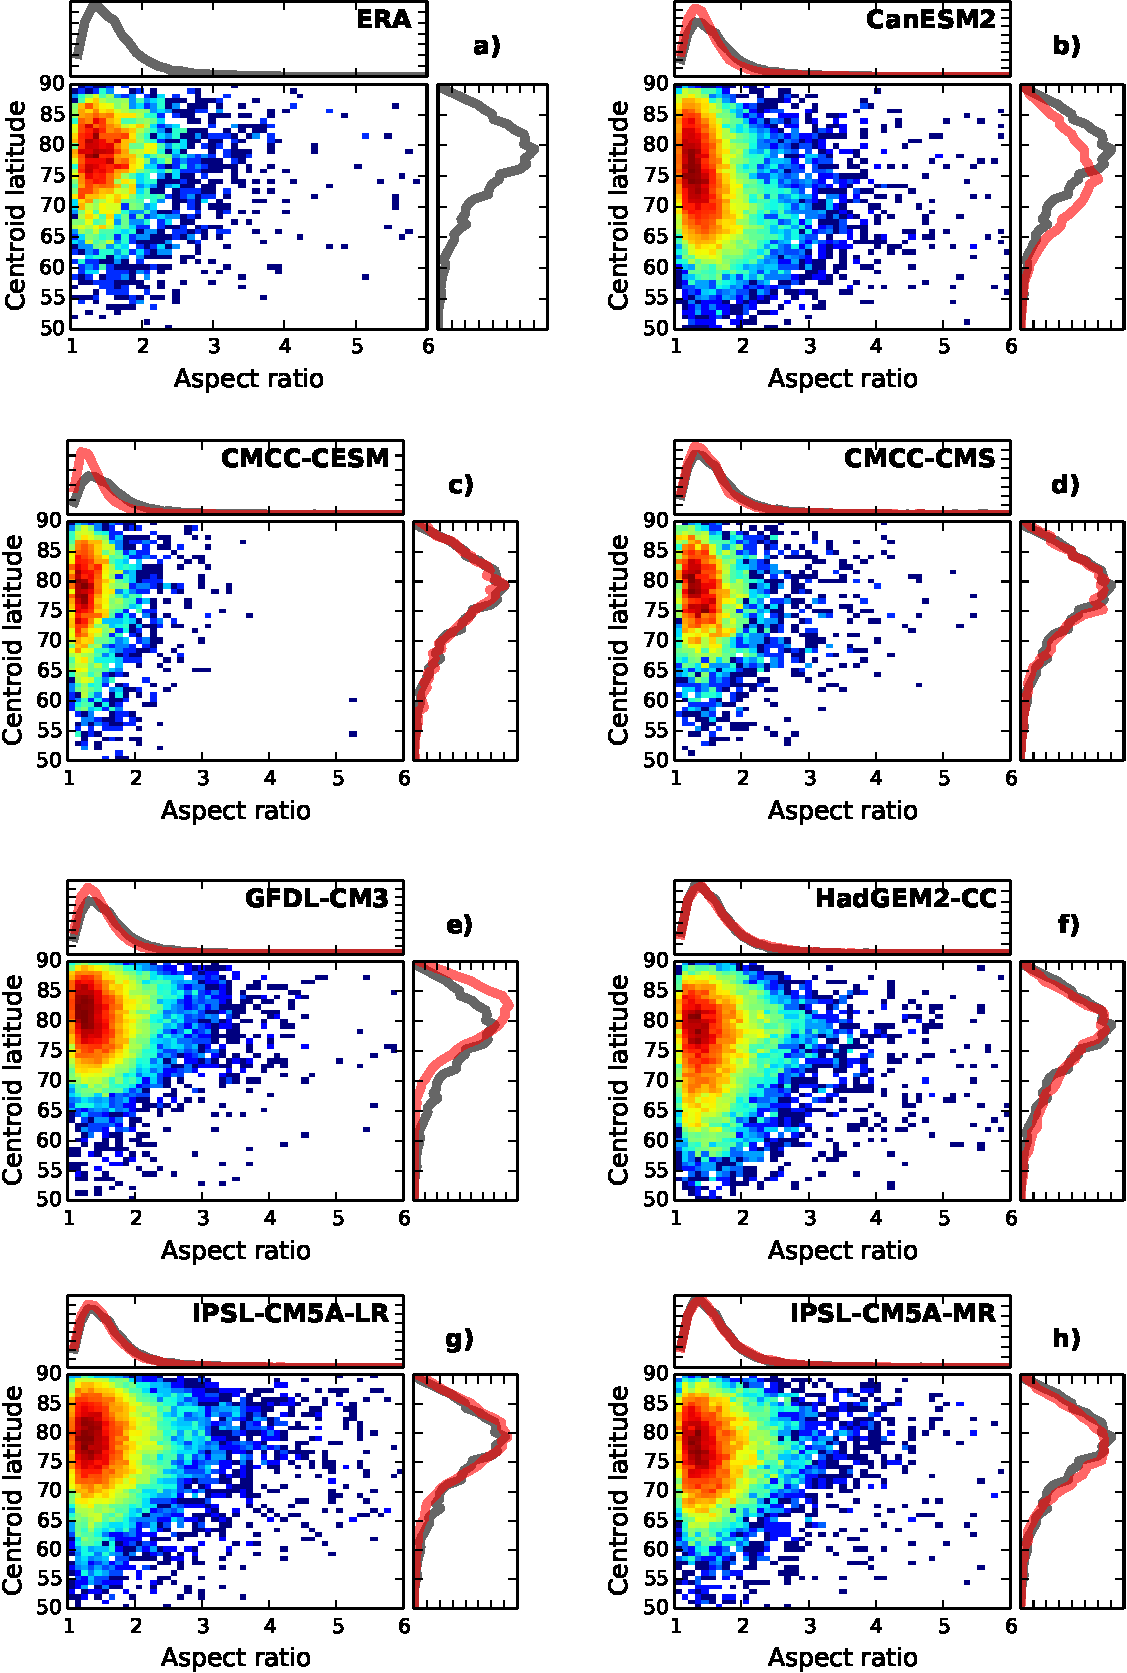
\includegraphics[width=\textwidth]{figures/chapter-models/moments_stats1.pdf}
 \caption[Distributions of moment diagnostics for the CMIP5
 models.]{Distributions of centroid latitude and aspect ratio for the ERA (grey
   lines) (a) and the CMIP5 models (red lines). Joint distributions are shown
   with a logarithmic scale such that red squares represent the densest
   regions.}
 \label{fig:cmip5_moments_stats}
\end{figure}

\begin{figure}[htbp]
 \ContinuedFloat
 \centering
 \noindent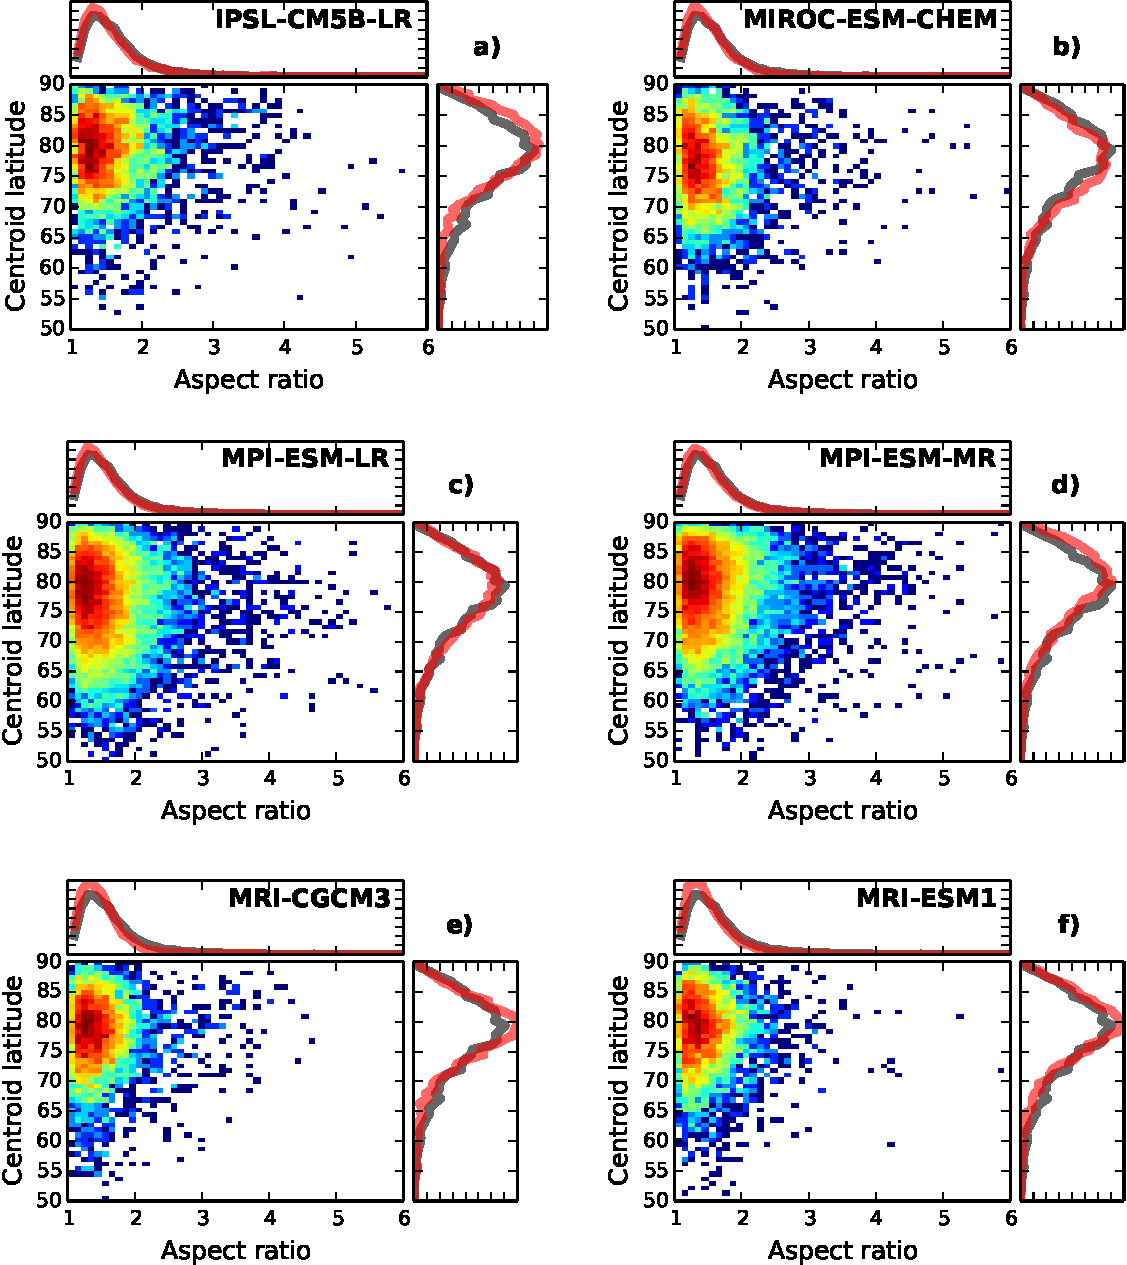
\includegraphics[width=\textwidth]{figures/chapter-models/moments_stats2.pdf}
 \caption[]{(Continued)}
\end{figure}


The centroid latitude and aspect ratio moment diagnostics are calculated for
each of the CMIP5 models over DJFM from the 10~hPa geopotential height field,
using the method described in Section \ref{sec:vort-geom-calc}. For each model
the value of the DJFM mean geopotential height at 60$^{\circ}$N and 10~hPa is
used to define the appropriate contour for the calculation of the moment
diagnostics. This accounts for biases in the mean geopotential height between
different models.

The resulting joint distributions of daily centroid latitude and aspect ratio
from each of the models are shown in Figure \ref{fig:cmip5_moments_stats}, along
with that from the ERA-40/ERA-Interim reanalysis (hereafter ERA) calculated in
Chapter \ref{cha:moments}. For each model the joint distribution histogram is
plotted with a logarithmic colour scale which is normalised according to the
number of days entering each box. As discussed in Chapter \ref{cha:moments}, it
can be seen that the joint distribution for ERA has an approximately triangular
distribution with high aspect ratio/poleward centroid latitude, and low aspect
ratio/equatorward centroid latitude being relatively more common than
high aspect ratio/equatorward centroid latitude. This shape of distribution is
well replicated by most of the models, although CanESM2 has a significantly
different shape, with the high aspect ratio/equatorward centroid latitude being
more common. 

No clear consistent biases among models emerge from this analysis. CanESM2 has a
modal centroid latitude which is about $5^{\circ}$ too far equatorward compared
to reanalysis. Contrastingly, GFDL-CM3 has a modal centroid latitude about
$2.5^{\circ}$ more poleward than observed. CMCC-CESM displays a clear bias in
the aspect ratio, with a distribution much less skewed towards high values than
in reanalysis.

The winter seasonal cycle of aspect ratio and centroid a latitude in the CMIP5
models is shown in Figure \ref{fig:cmip5_moments_stats_seas}. For the mean
aspect ratio and centroid latitude, the majority of models agree well with
reanalysis. CMCC-CESM has a consistently too low mean aspect ratio, while
GFDL-CM3 has a consistently too poleward mean centroid latitude, indicating that
these biases are not strongly seasonally dependent. On the other hand, the large
equatorward bias in the CanESM2 mean centroid latitude is much larger in
December and early January than later in winter. The 95th percentile of aspect
ratio is lower than reanalysis for the majority of models throughout the season,
indicating that models have, on average, too little variability in aspect ratio
 
\begin{figure}
 \centering
 \noindent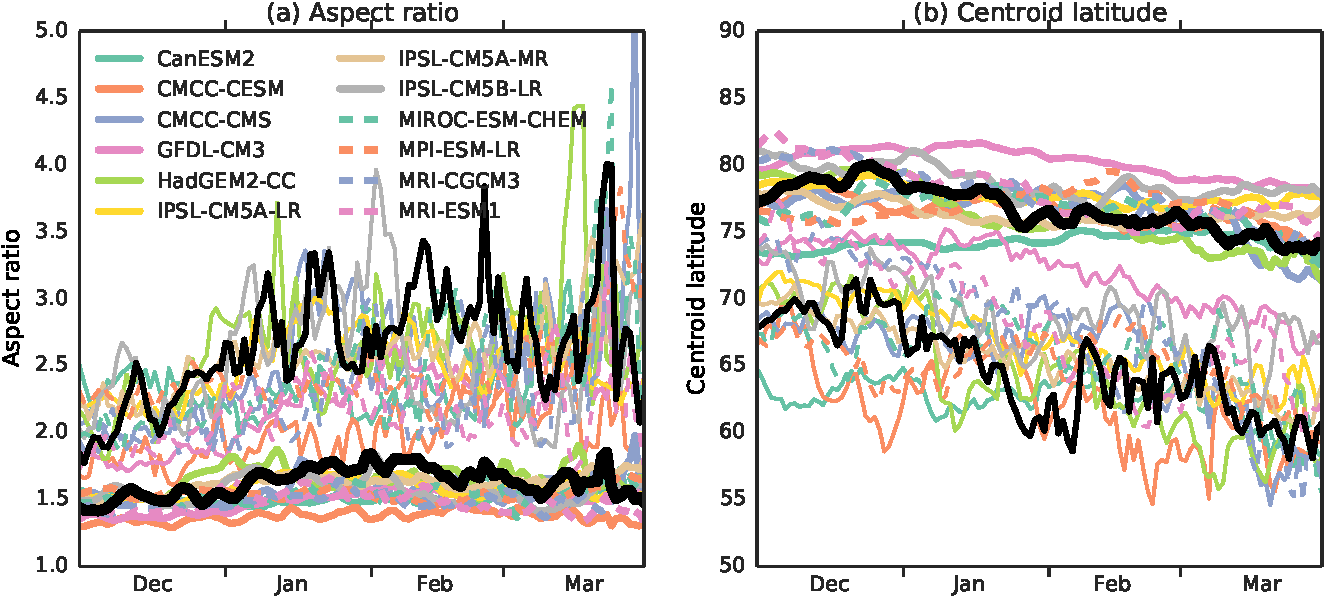
\includegraphics[width=\textwidth]{figures/chapter-models/moments_seasonal_stats.pdf}
 \caption[Seasonal cycle of moment diagnostics in the CMIP5 models]{Seasonal
   cycle of aspect ratio and centroid latitude in ERA (black) and the CMIP5
   models (colours). Thick lines represent the mean and thin lines the 95th or
   5th percentile for aspect ratio and centroid latitude respectively.}
 \label{fig:cmip5_moments_stats_seas}
\end{figure}


\subsection{Displaced and split vortex events}

Displaced and split vortex events are identified within the CMIP5 ensemble using
the threshold-based method described in Section \ref{sec:event-definition}. The
same thresholds as used for ERA (66$^{\circ}$N for centroid latitude and 2.4 for
aspect ratio) are used for the models in order to identify, as much as possible,
geometrically equivalent events. The same persistence of 7 days was also used.
The frequency of displaced and split vortex events for each model is shown in
Figure \ref{fig:cmip5_events_bar_stacked}.

\begin{figure}[htbp]
 \centering
 \noindent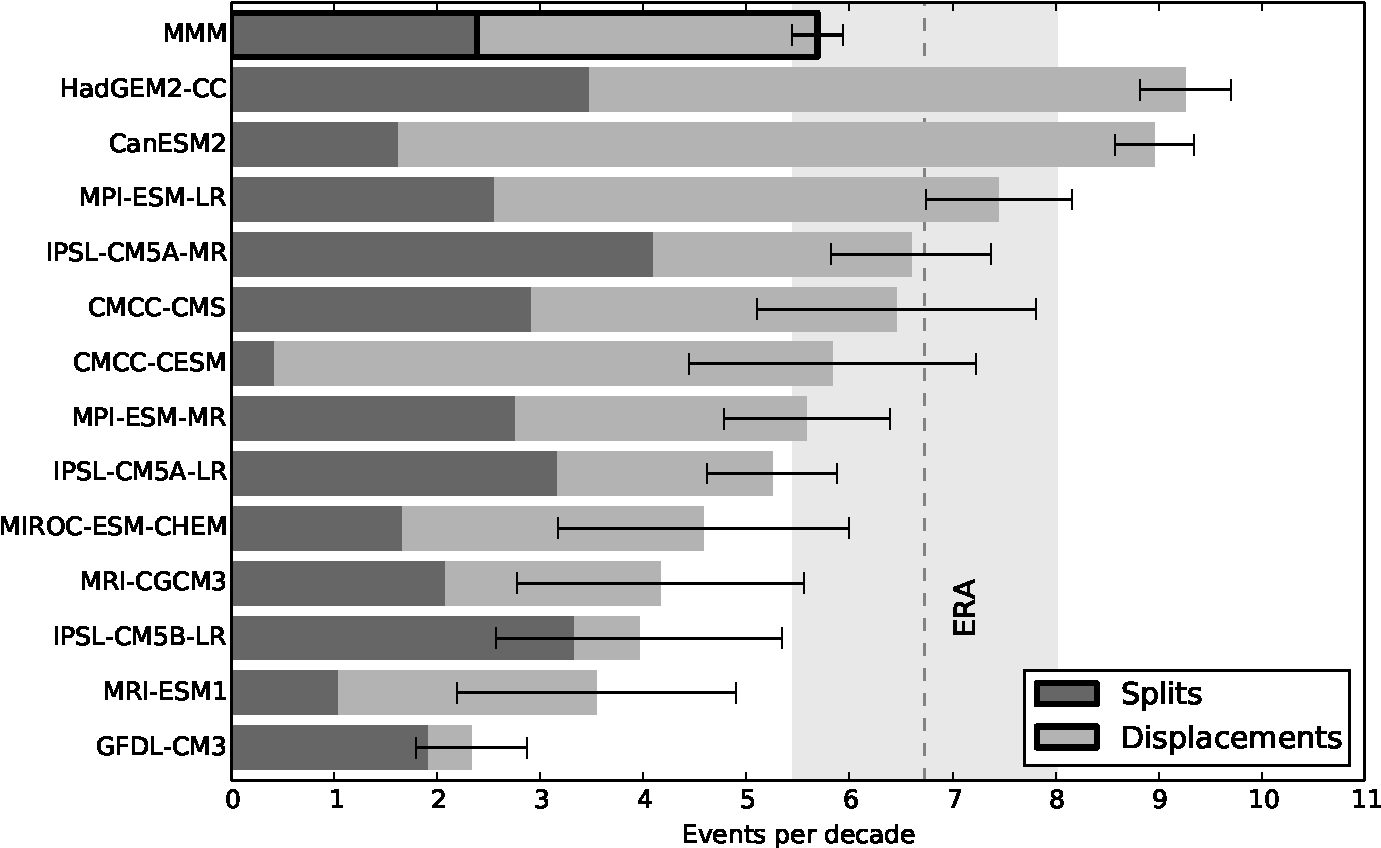
\includegraphics[width=\textwidth]{figures/chapter-models/events_bar_stacked.pdf}
 \caption[Frequency of split and displaced vortex events in the CMIP5
 models]{Frequency of split and displaced vortex events in the CMIP5 models,
   ERA, and the multi-model mean (MMM). Error bars are for the frequency of all
   events, and represent one $\sigma$ range, assuming a binomial distribution of
   events. The grey shaded region represents the one $\sigma$ range for ERA,
   along with the mean (dashed line.) }
 \label{fig:cmip5_events_bar_stacked}
\end{figure}

The total frequency of displaced and split vortex events for each of the CMIP5
models agrees well with the equivalent SSW frequency calculated by
\citet{Charlton-Perez2013}, who identified events based on the reversal of
zonal-mean zonal wind at 60$^{\circ}$N and 10~hPa. They also found HadGEM2-CC to
have the highest frequency of events within the CMIP5 ensemble, while MRI-CGCM3
is the model with the lowest frequency of SSWs in their study (excluding GFDL-CM3
and MRI-ESM1 which \citet{Charlton-Perez2013} did not analyse, MRI-CGCM3 is the
second-lowest frequency in the present study). This similarity between
\citet{Charlton-Perez2013} and the present study indicates that the close
relationship between moment diagnostics-defined events and SSWs defined by
zonal-mean zonal wind, as described in Chapter \ref{cha:moments}, also holds for
climate models (although this is not explicitly studied here).

As well as the large differences in the total frequency of displaced and split
vortex events, it can be seen in Figure \ref{fig:cmip5_events_bar_stacked} that
the ratio of frequencies of these events varies significantly between
models. For instance CanESM2 and CMCC-CESM simulate almost entirely displaced
vortex events, while IPSL-CM5B-LR and GFDL-CM3 simulate almost entirely split
vortex events. In the multi-model mean (MMM) these biases largely cancel, to
give a approximately equal ratio of displaced to split vortex events, which is
in agreement with reanalysis.

The seasonal distribution of these displaced and split vortex events is
illustrated in Figure \ref{fig:cmip5_events_seasonal}. Some models (CMCC-CMS,
HadGEM2-CC and IPSL-CM5A-LR) replicate the observed distribution, with split
vortex events being more likely in early winter, and displaced vortex events in
late winter. Other models, however, have a very different
distribution of events. CanESM2, CMCC-CESM and MPI-ESM-LR all show little
seasonal variability in the frequency of events. 


\begin{figure}
 \centering
 \noindent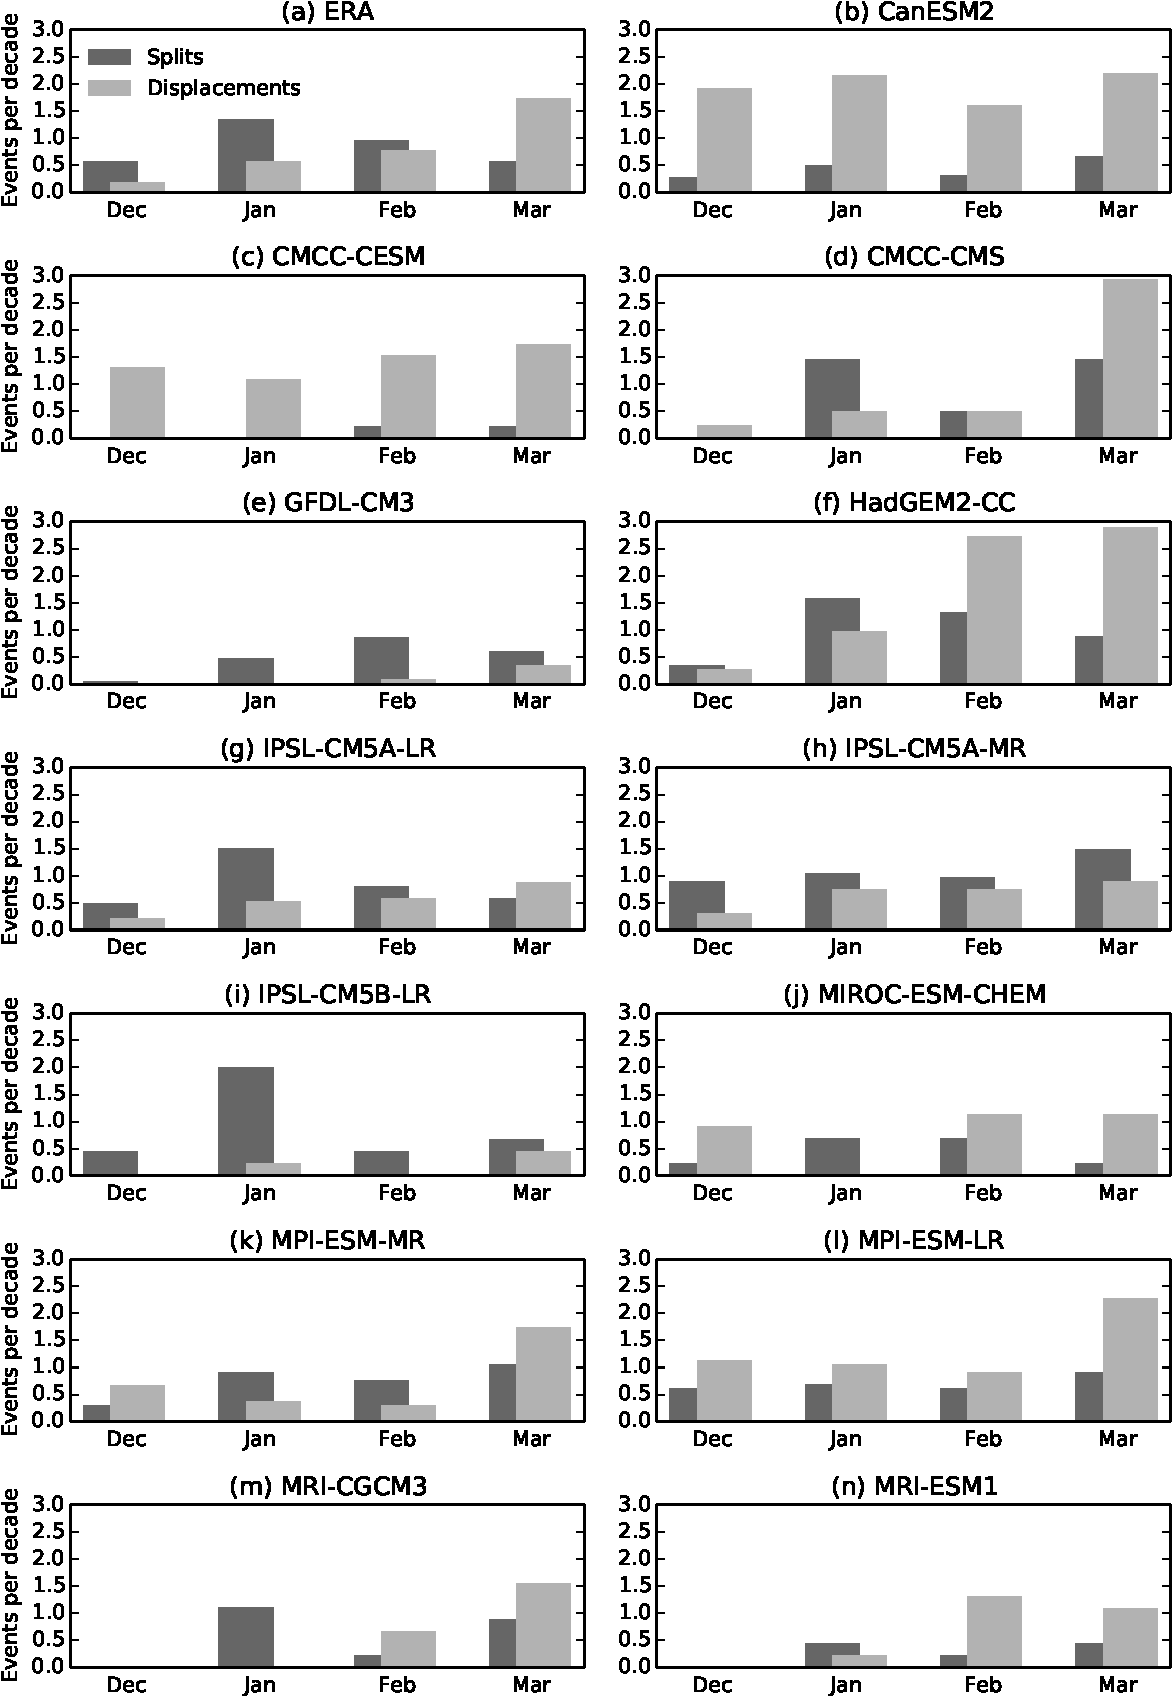
\includegraphics[width=\textwidth]{figures/chapter-models/events_seasonal.pdf}
 \caption[Seasonal distribution of splits and displacements in the CMIP5
 models]{Seasonal distribution of the occurrence of split and displaced vortex
   events in ERA (a) and the CMIP5 models.}
 \label{fig:cmip5_events_seasonal}
\end{figure}

\bigskip It is now considered how model biases in the climatology of the
stratospheric polar vortex, discussed in Section \ref{sec:moment-diagnostics},
affect the frequency of split and displaced vortex events. The climatological
average state of the vortex is defined by the mode -- the peak of the
probability distribution function -- of the aspect ratio and centroid
latitude. Unlike the mean, this quantity is not affected by extreme values and
it represents the average undisturbed state of the vortex. The peak can be
estimated by the maximum value of a histogram, however this introduces
significant random errors and is sensitive to the selection of bin size. A more
accurate estimation of the mode can be made by fitting the aspect ratio and
centroid latitude with a theoretical distribution and then finding the peak of
that distribution. Following \citet{Mitchell2011}, we fit the aspect ratio with
a generalised extreme value (GEV) distribution of the form
\begin{equation}
f(x;\mu,\sigma,\xi) = \frac{a^{(-1/\xi)-1}}{\sigma}\mathrm{e}^{{-a}^{-1/\xi}}
\quad , 
\end{equation}
with
\begin{equation} 
a = 1 + \xi \frac{x-\mu}{\sigma} \quad ,
\end{equation}
where $\mu$ determines the position of the peak along the $x$-axis, $\sigma$
determines the variance of the distribution and $\xi$ the skewness. These
parameters are determined using the method of maximum-likelihood estimation
\citep{Wilks}. This method is also used to fit a Gaussian distribution of the
form
\begin{equation}
f(x;\mu,\sigma) = \frac{1}{\sigma\sqrt{2\pi}} \left(
  -\frac{(x-\mu)^2}{2\sigma^{2}} \right) \quad ,
\end{equation}
where $\mu$ determines the position of the peak along the $x$-axis and $\sigma$
is the standard deviation, to the cube of the centroid latitude, and then the
cube root taken to return the original distribution. \citet{Mitchell2011} found
that these distributions accurately fit the histograms of centroid latitude and
aspect ratio in reanalysis data, apart from the extreme tails of the
distribution. Qualitative inspection of the distribution for each model confirms
that they also provide a similarly good fit to each of the model's histograms.

Figure \ref{fig:cmip5_moments_scatter} shows the relationship between the modal
aspect ratio and centroid latitude and frequency of split and displaced vortex
events. It can be seen that strong linear relationships exist; the modal aspect
ratio accounts for 79\% of the variance in the frequency of split vortex events
and the modal centroid latitude accounts for 76\% of the variance in the
frequency of displaced vortex events. This demonstrates that biases in the
average undisturbed state of the vortex account for the vast majority of
inter-model spread in the representation of extremes. An implication of this is
that the models are consistent in their representation of the variability of
aspect ratio and centroid latitude, relative to the model climatology.

It can also be seen in Figure \ref{fig:cmip5_moments_scatter} that the values
for ERA lie very close to the best fit lines of the CMIP5 models. This implies
that the accuracy of a model's representation of the frequency of displaced and
split vortex events can be significantly improved by a more accurate average
undisturbed vortex state. Furthermore, while the ERA value for modal centroid
latitude lies approximately in the middle of that for the CMIP5 models, only two
models have a larger modal aspect ratio than ERA, indicating that a too
circularly-symmetric vortex is a common bias among models.

\begin{figure}
 \centering
 \noindent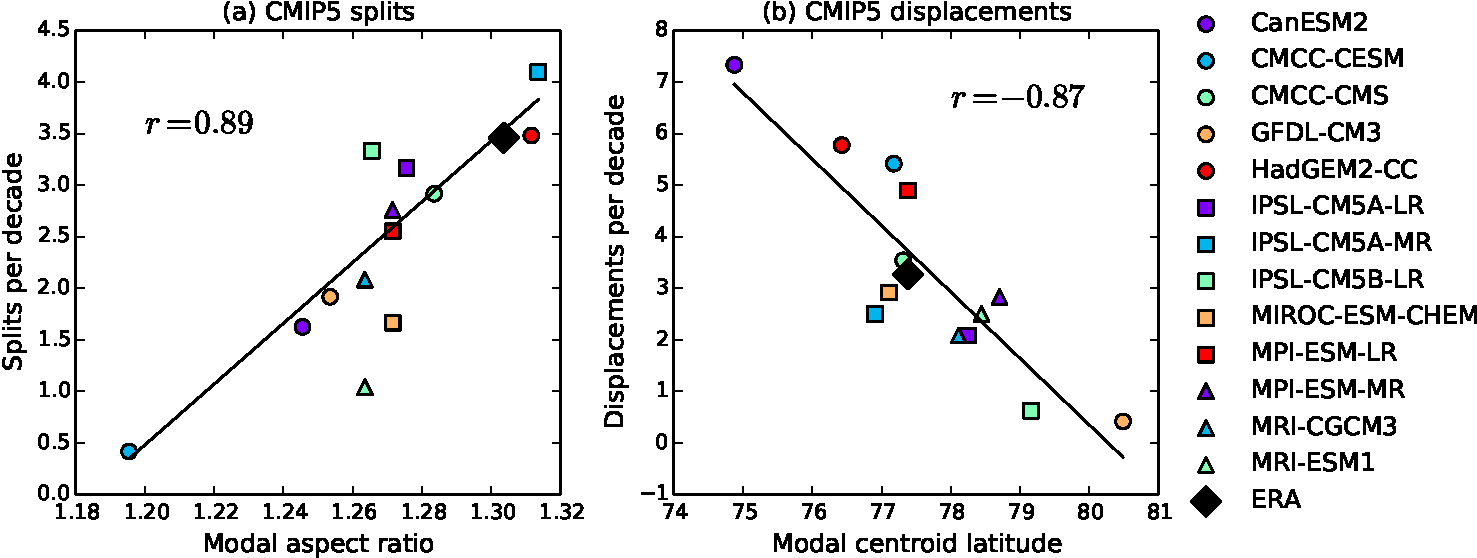
\includegraphics[width=\textwidth]{figures/chapter-models/CMIP5_moments_scatter.pdf}
 \caption[Comparison of moment diagnostics and frequency of split and displaced
 vortex events.]{Comparison of the DJFM mean aspect ratio with frequency of
   split vortex events (a) and DJFM mean centroid latitude with frequency of
   displaced vortex events (b) in the CMIP5 ensemble and ERA. Linear best fits
   and the correlation coefficients for all the models are also shown.}
 \label{fig:cmip5_moments_scatter}
\end{figure}

The structure of the stratospheric polar vortex during split and displaced
vortex events in the CMIP5 ensemble is shown in Figure
\ref{fig:10hPa_GPH_comp}. This displays composites of 10~hPa geopotential height
at the onset date of the events for each model. It can be seen that the majority
of models accurately reproduce splitting events as occurring along the
$90^{\circ}$W-$90^{\circ}$E axis, and displacement events with a vortex shifted
towards Scandinavia and Siberia. CanESM2 is an exception to this, with split
vortex events which are elliptical but centred quite far from the pole. The
IPSL-CM5B-LR model also has a very different appearance of displaced vortex
events, although this composite only consists of three events so differences are
unlikely to be statistically significant. There is also significant inter-model
spread in the relative strengths of the Aleutian and Azores highs during split
vortex events. Several models (GFDL-CM3, IPSL-CM5A-LR, IPSL-CM5B-LR, MRI-ESM1)
show an approximately equal strength Aleutian and Azores highs, while others
(CMCC-CMS, HadGEM2-CC, IPSL-CM5A-MR, MPI-ESM-LR, MPI-ESM-MR, MRI-CGCM2) show a
weaker Azores high, which is in closer agreement with reanalysis. The more
symmetrical Aleutian and Azores highs indicate a greater dominance of wave-2
activity in split vortex events than is found in observations, where not all
split vortex events are dominated by wave-2 activity
\citep{Waugh1997,Mitchell2013}.

\begin{figure}
 \centering
 \noindent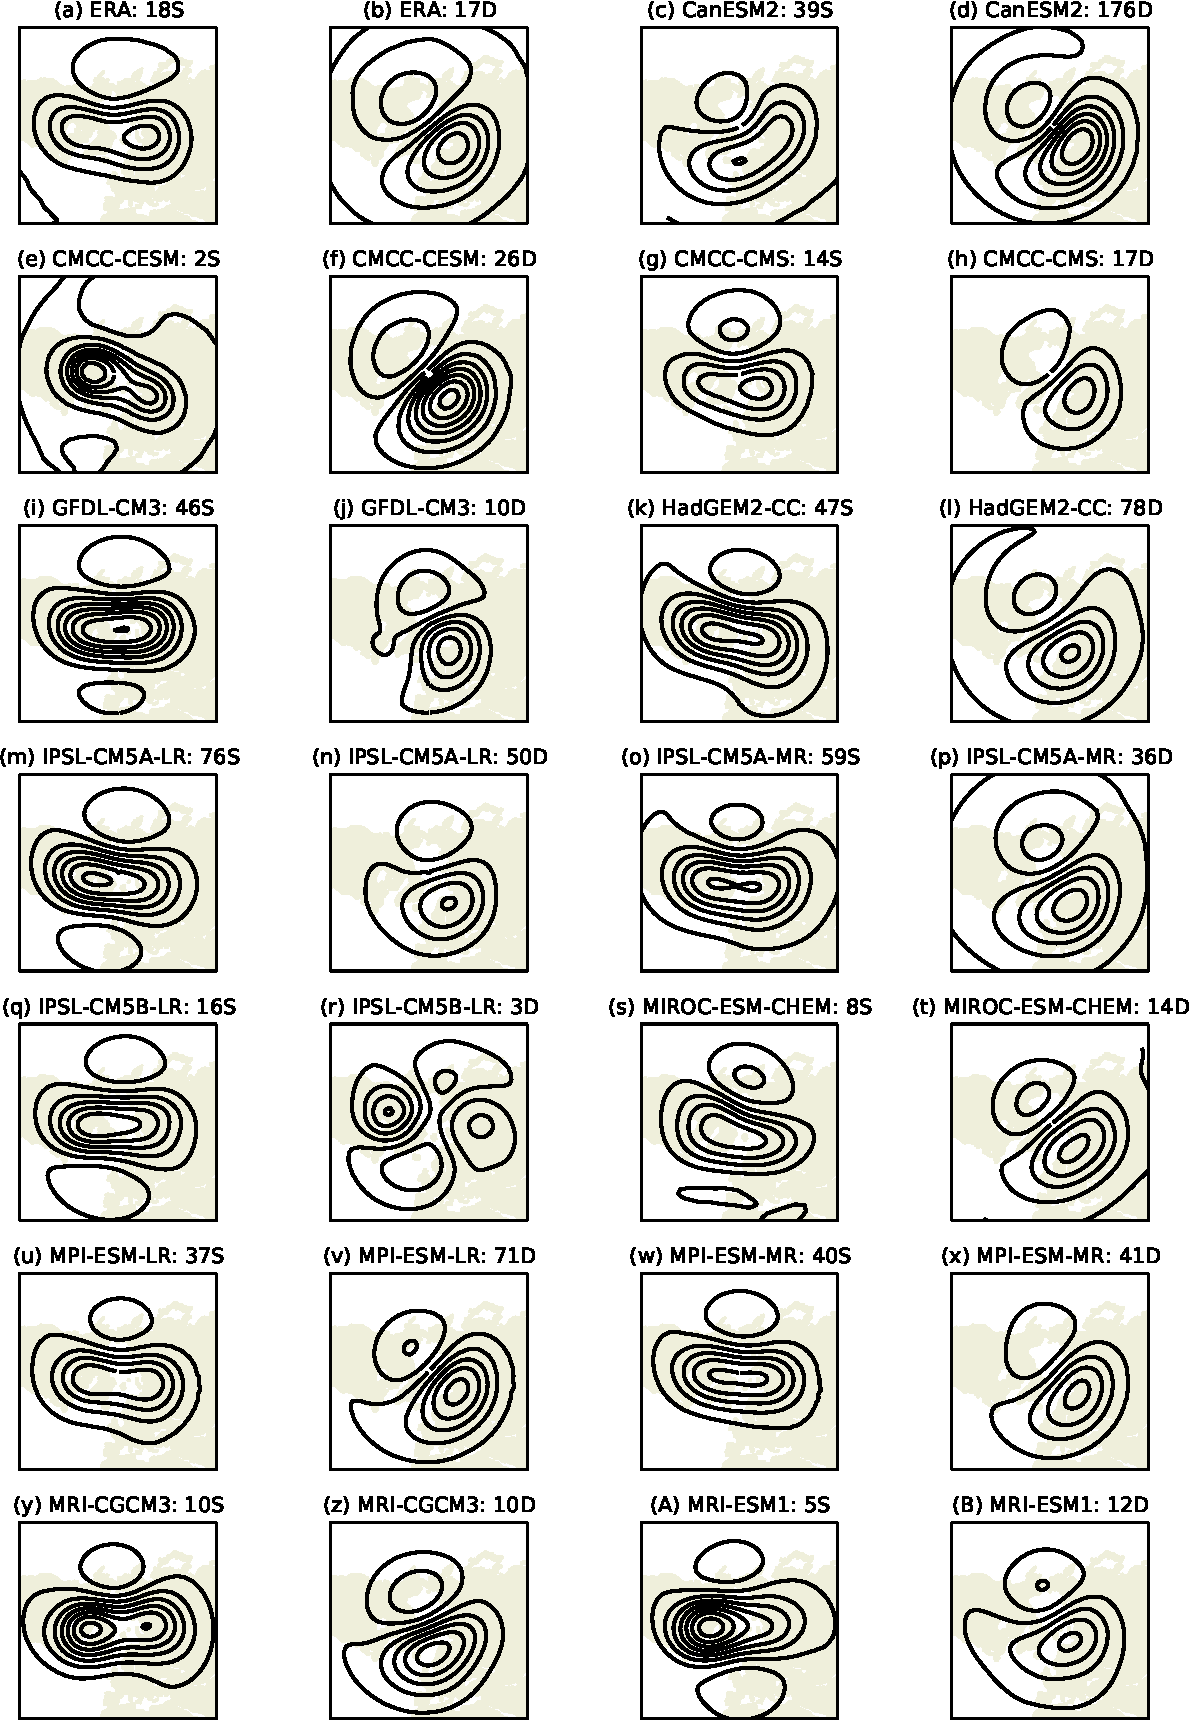
\includegraphics[width=\textwidth]{figures/chapter-models/10hPa_GPH_composites.pdf}
 \caption[Composites of 10~hPa $Z$ at the onset date split and displaced vortex
 events in the CMIP5 models.]{Composites of 10~hPa $Z$ at the onset date of
   split (S) and displaced (D) vortex events in ERA (a,b) and the CMIP5
   models. The number of events entering the composite and their type are
   shown in the title of each plot. The contour interval is 0.3~km.}
 \label{fig:10hPa_GPH_comp}
\end{figure}




\section{Stratosphere-troposphere coupling}
\subsection{Zonal-mean response to displaced and split vortex events}

The time-height evolution of the atmosphere around split and displaced vortex
events in each of the CMIP5 models is displayed in Figure
\ref{fig:cmip5_dripping_paint}. This shows composites of polar cap
($60^{\circ}$-$90^{\circ}$N) geopotential height ($Z$) anomalies from 90 days
before to 90 days following events. The anomalies are calculated from the
climatology of each day for each model. The figures extend downwards only to
500~hPa (rather than 1000~hPa). This is because models differ in their
representation of geopotential height which is below ground level; some allow
negative values, while others set this as an undefined value. This introduces
significant errors in the calculation of a climatology and anomalies at levels
where the geopotential height is occasionally below ground level. Polar cap $Z$
is highly correlated with the NAM (calculated from zonal mean $Z$ according to
the method of \citet{Baldwin2009}) over the levels shown in Figure
\ref{fig:cmip5_dripping_paint}. Indeed, comparing Figures
\ref{fig:cmip5_dripping_paint} (a) and (b) with Figure \ref{fig:dripping_paint}
shows that the ERA composites for polar cap $Z$ and the NAM are very similar. In
Figure \ref{fig:cmip5_dripping_paint} the number of events entering each
composite is shown in the upper right-hand corner, and it should be noted that
composites of a small number of events are likely to be subject to significant
statistical uncertainty.

It can be seen that there are large inter-model differences in the evolution of
polar cap $Z$ following split and displaced vortex events. For some models
(e.g. CanESM2, CMCC-CMS) lower stratospheric anomalies persist for about 45
days, similar to reanalysis, while for others (e.g. IPSL-CM5A-LR, GFDL-CM3)
these persist for much longer, beyond 60 days. There are also differences in the
stratospheric precursors to events; while some models (e.g. CanESM2, GFDL-CM3,
MRI-CGCM3) simulate a stronger negative anomaly prior to displacement events,
similar to reanalysis, others (HadGEM2-CC, IPSL-CM5A-MR, MRI-ESM1), show more
negative anomalies prior to split vortex events. 

Most significantly, there is a large spread in the tropospheric anomalies over
the 10-90 days following split and displaced vortex events. Several models
(e.g. IPSL-CM5A-LR, IPSL-CM5A-MR, MPI-ESM-LR) show only very weak anomalies
below approximately 200~hPa, while others (e.g., CMCC-CESM, GFDL-CM3, MRI-ESM1)
show stronger anomalies. Among those models which do show stronger tropospheric
anomalies, there are also differences in the relative magnitude following split
and displaced vortex events. For instance, for GFDL-CM3, and MRI-ESM1
tropospheric anomalies following displaced vortex events are stronger, while for
MIROC-ESM-CHEM and MPI-ESM-MR anomalies following split vortex events are
stronger, in closer agreement with reanalysis. 

As well as these large inter-model differences, there are also some consistent
features among models. Almost all models show a barotropic onset to split vortex
events, with anomalies occurring at the same time throughout the depth of the
atmosphere. In contrast, displaced vortex events apprear more baroclinic, with
onset occurring first near the uppermost level. This is consistent with the
difference found in reanalysis, indicating that this is likley to be a robust
difference between the response to split and displaced vortex events. These
features are also apparent in the multi-model mean (MMM) (Figures
\ref{fig:cmip5_dripping_paint} C and D). This mean is calculated so as to give
each event an equal weight (rather than each model), and so does not give undue
weight to models with only a small number of events. On the other hand this does
mean that greater weight is given to models with more ensemble members and more
events (almost one third of all displaced vortex events come from CanESM2), but
the difference in baroclinicity of split and displaced vortex events is observed
to be very consistent among models.

\begin{figure}
 \centering
 \noindent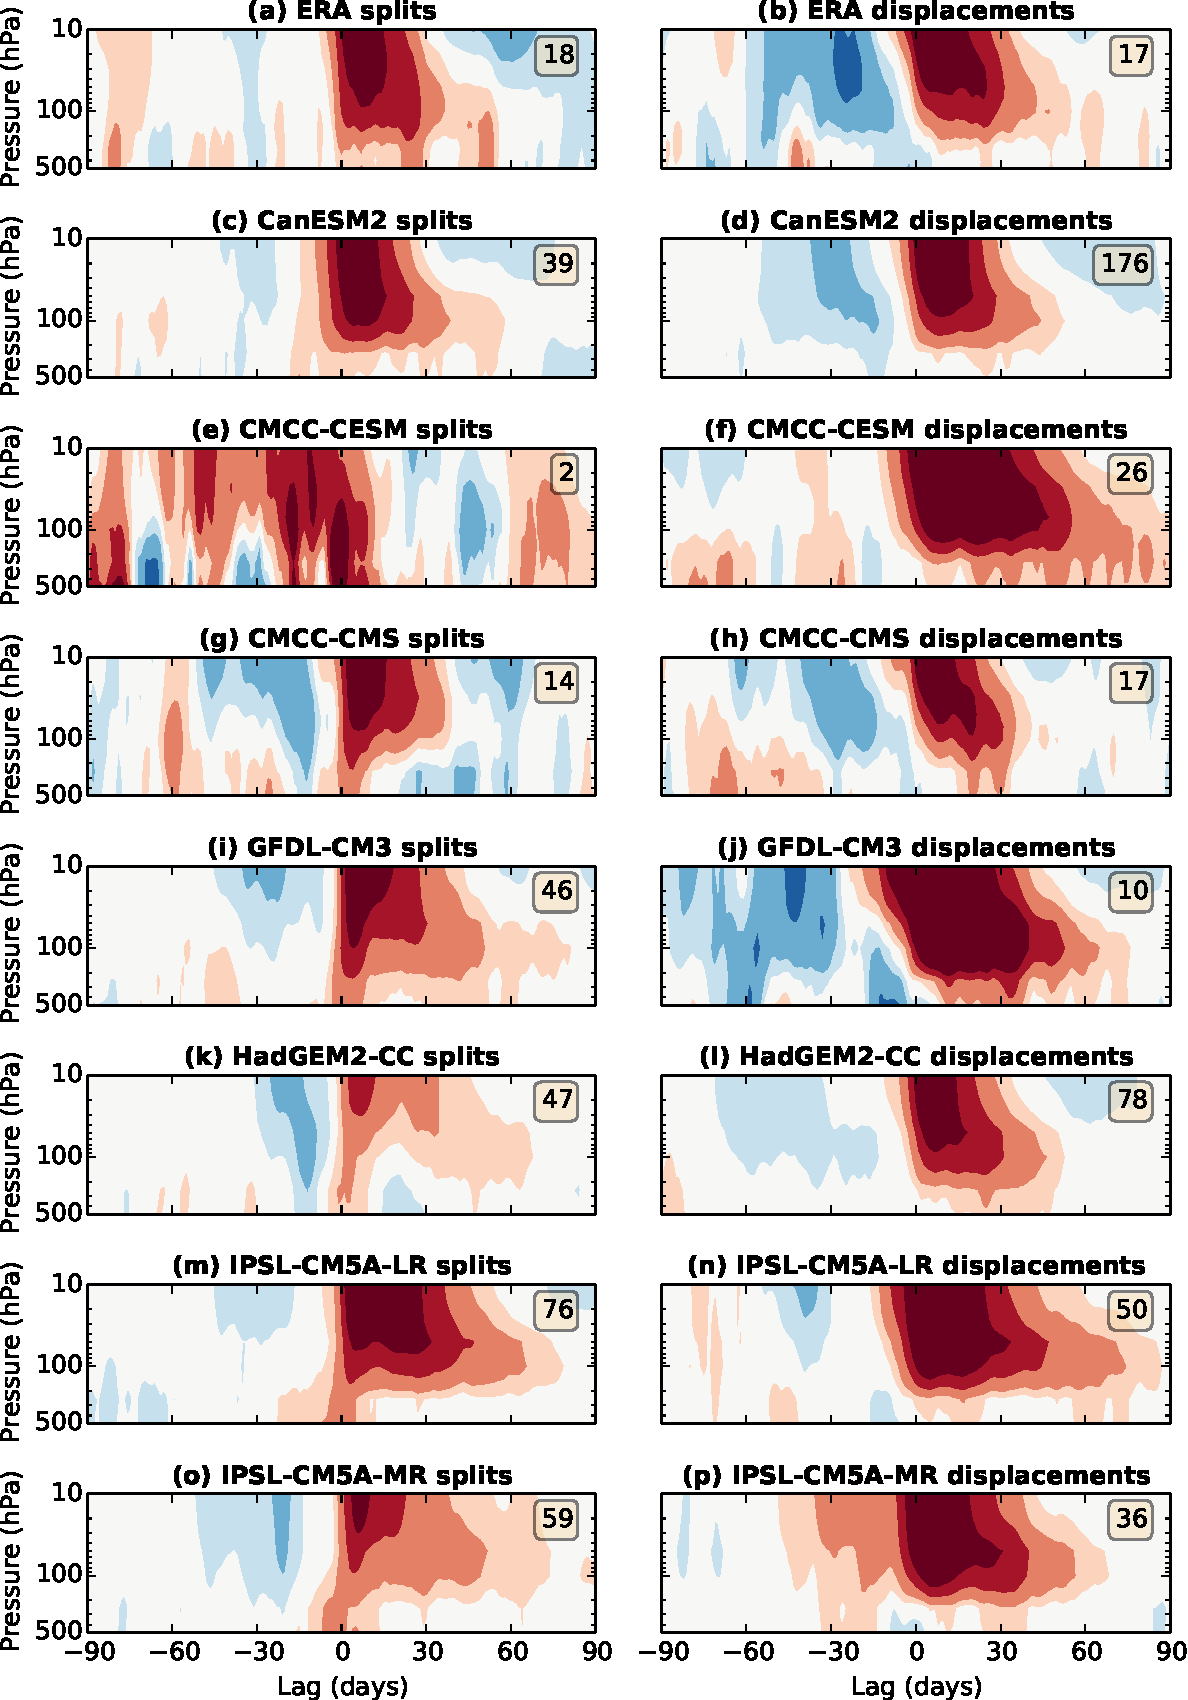
\includegraphics[width=\textwidth]{figures/chapter-models/dripping_paint1.pdf}
 \caption[NAM composites for splits and displacements in the CMIP5
 models]{Composites of normalised polar cap averaged $Z$ anomalies following
   split and displaced vortex events in ERA (a,b), the CMIP5 models, and the
   multi-model mean (C,D). Numbers in the upper right of each plot represent the
   number of events entering the composite.}
 \label{fig:cmip5_dripping_paint}
\end{figure}

\begin{figure}
 \ContinuedFloat
 \centering
 \noindent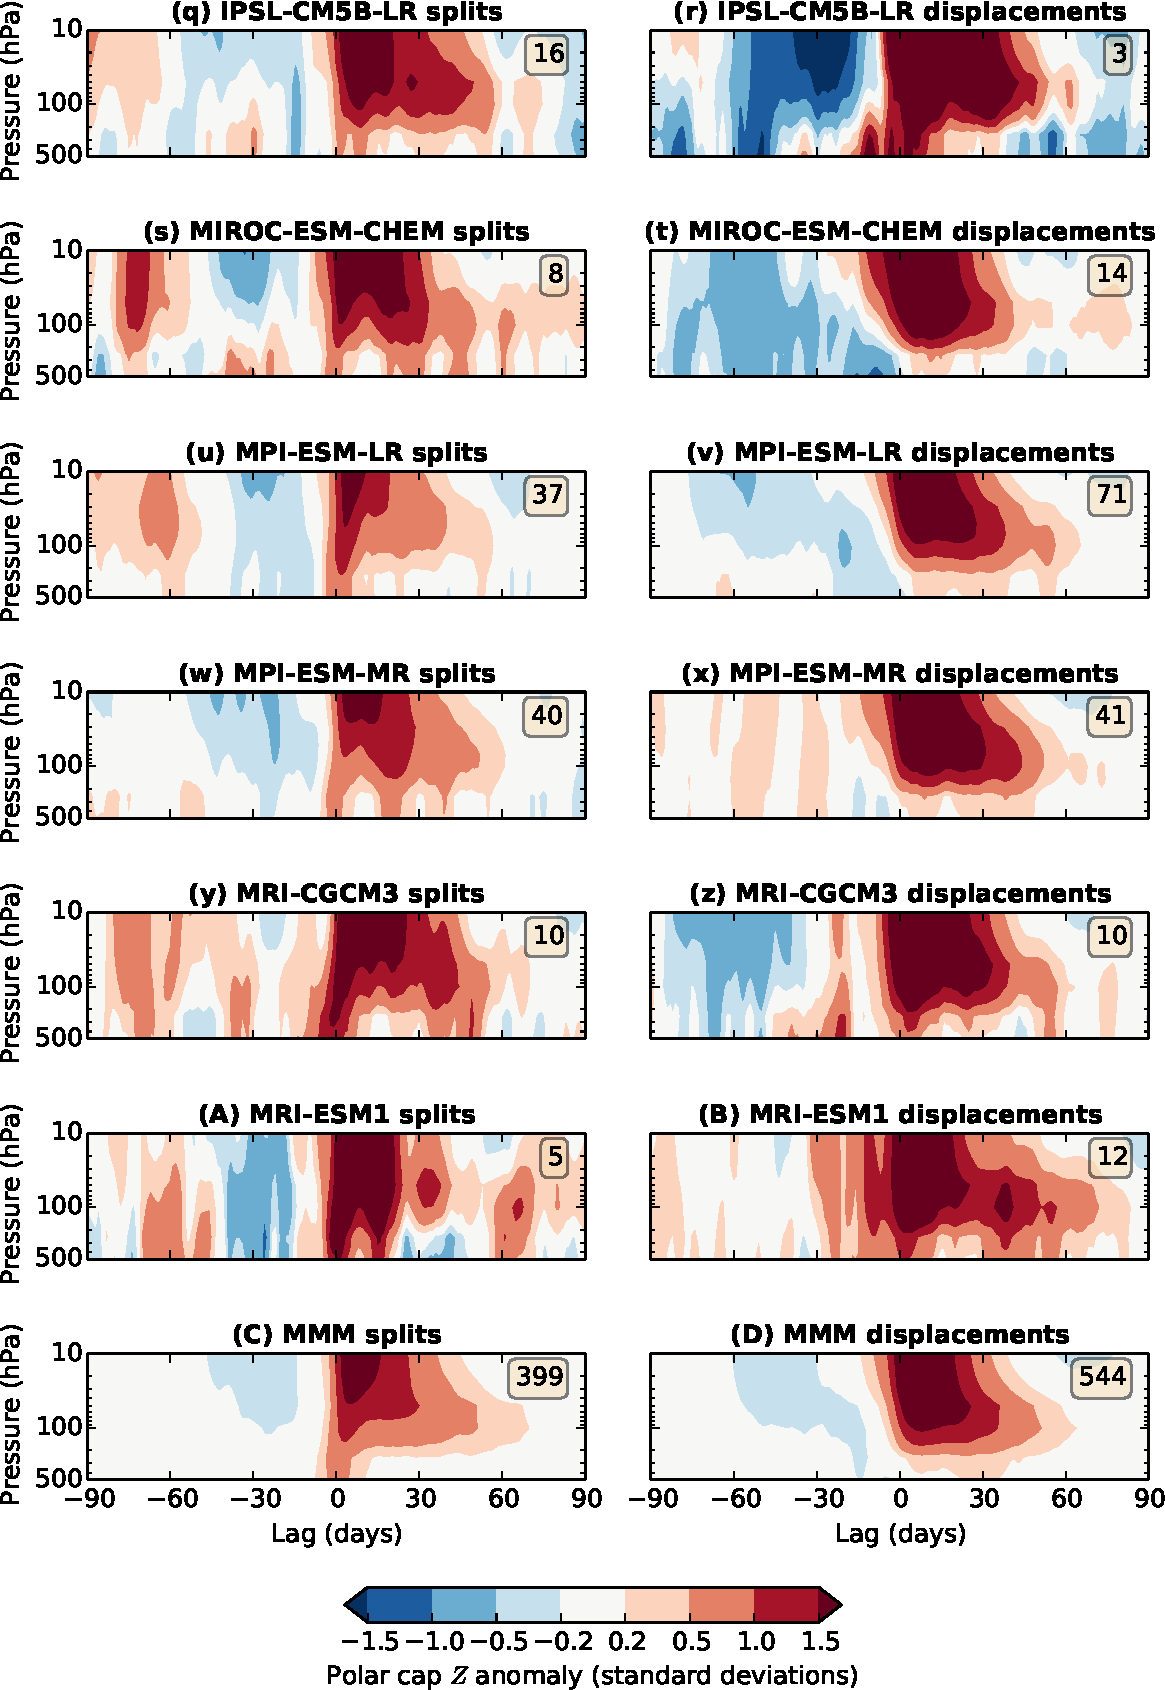
\includegraphics[width=\textwidth]{figures/chapter-models/dripping_paint2.pdf}
 \caption[]{(Continued)}
\end{figure}


\subsection{Spatial response to displaced and split vortex events}

\begin{figure}
 \centering
 \noindent\includegraphics[width=\textwidth]{figures/chapter-models/mslp_composites.pdf}
 \caption[MSLP composites following splits and displacements in the CMIP5
 models]{Composites of mean sea-level pressure anomalies averaged 0-30 days
   following split (S) and displaced (D) vortex events in the CMIP5
   ensemble. Also shown are the ERA composite (a,b) and the multi-model mean
   (C,D). The multi-model mean is calculated as to give each event an equal
   weighting.}
 \label{fig:cmip5_mslp_comp}
\end{figure}

\begin{figure}
 \centering
 \noindent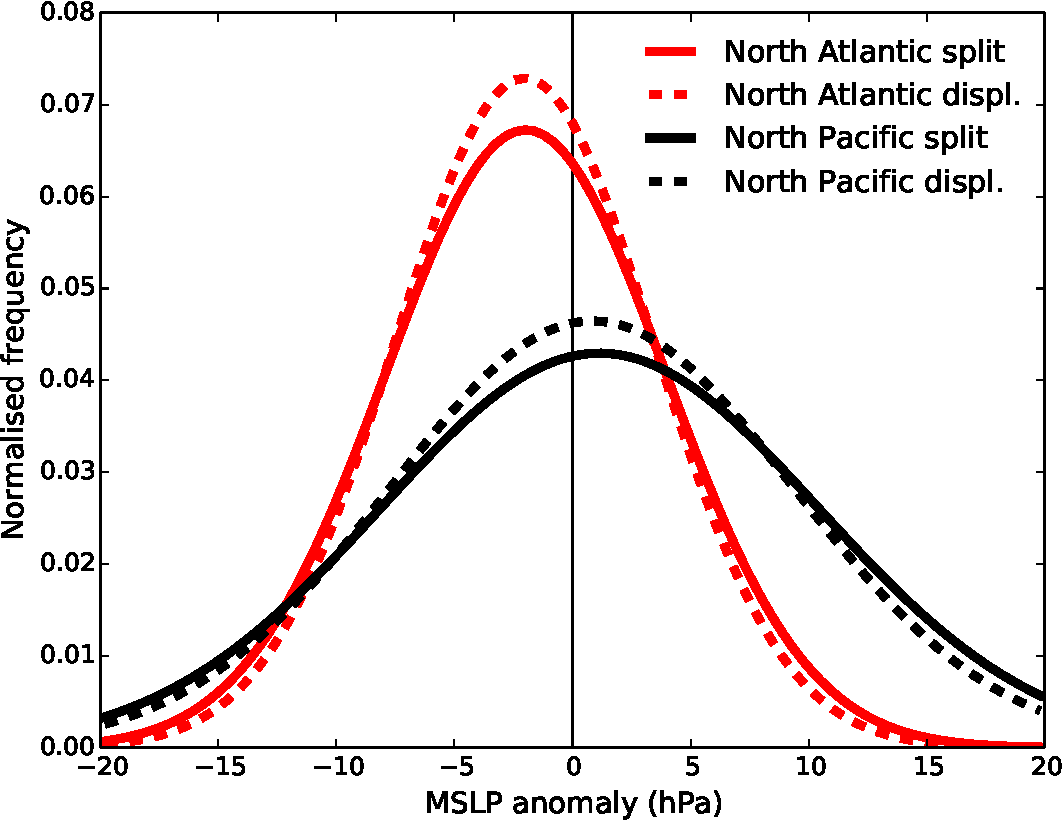
\includegraphics[width=0.7\textwidth]{figures/chapter-models/NAO_PNA_histogram.pdf}
 \caption[Distribution of MSLP anomalies in North Pacific and Atlantic following
 splits and displacements.]{Distribution of mean sea-level pressure anomalies in
   the central North Atlantic ($38^{\circ}$N, $26^{\circ}$W) and central North
   Pacific ($45^{\circ}$N, $165^{\circ}$W) averaged over the 30 days following
   split and displacement events in all the CMIP5 models. These two locations
   correspond to centres of action of the NAO and PNA patterns
   respectively. Data are fitted with a Gaussian distribution.}
 \label{fig:cmip5_nao_pna}
\end{figure}

Mean sea-level pressure (MSLP) anomalies averaged over the 30 days following
split and displaced vortex events for each of the CMIP5 models are displayed in
Figure \ref{fig:cmip5_mslp_comp}. Also shown are the anomalies for ERA (a,b)
(the same as Figure \ref{fig:mslp_composites}) as well as the multi-model mean
(c,d), again calculated so as to give each event an equal weight. The
climatology from which anomalies are calculated is determined by a 10-day
running mean of the average for each day of the year at each spatial
location. The number of events entering each composite is shown, and again, care
must be taken interpreting composites of a small number of events due to
statistical uncertainty.

Following both split and displaced vortex events, all models show a positive
MSLP anomaly near the North Pole, and a negative anomaly centred over Western
Europe and the North Atlantic. This pattern is consistent with a negative
projection onto the North Atlantic Oscillation. Less consistent among models are
anomalies over the North Pacific; many models (e.g. MRI-CGCM3, IPSL-CM5A-LR)
show positive anomalies, while MPI-ESM-LR a MPI-ESM-MR have negative anomalies
following both split and displaced vortex events. MIROC-ESM-CHEM has different
sign anomalies in the North Pacific following split (negative) and displaced
(positive) vortex events. In the multi-model mean, a weakly positive North
Pacific anomaly is seen.

Figure \ref{fig:cmip5_nao_pna} illustrates that this difference in consistency
of the Atlantic and Pacific MSLP anomalies also exists in the multi-model
ensemble of all events. It shows the distribution of MSLP anomalies averaged 30
days following all modelled split and displaced vortex events at the approximate
centres of action of the NAO (over the Azores at $38^{\circ}$N, $26^{\circ}$)
and the Pacific-North American (PNA) pattern (central North Pacific at
$45^{\circ}$N, $165^{\circ}$W). The North Atlantic distribution is centred
further from zero and has a lower variance than the North Pacific distribution
for both split and displaced vortex events. This is despite the fact that the
standard deviation in monthly winter MSLP is approximately equal in the two
regions \citep{Allan2006}, and so again indicates the more consistent North
Atlantic response.

This inconsistency in the Pacific anomalies has important consequences for the
interpretation of zonal mean anomalies following split and displaced vortex
events. For instance, the IPSL-CM5A-LR model shows weak tropospheric anomalies
(relative to other models) of polar cap averaged $Z$ following split and
displaced vortex events (Figure \ref{fig:cmip5_dripping_paint} (m,n)), but a
relatively strong NAO signal (Figure \ref{fig:cmip5_mslp_comp} (m,n)),
particularly following split vortex events. The reason for this difference is
that the model also shows relatively strong positive North Pacific anomalies,
that to some extent cancel the North Atlantic anomalies in the polar cap
average. Such an effect would also be seen in the NAM, even if calculated from
non zonally-averaged $Z$, since the surface NAM pattern (the leading EOF of
MSLP) has centres of action of the same sign in the North Atlantic and North
Pacific \citep[e.g.,][]{Ambaum2001}.

A robust difference found between MSLP anomalies following split and displaced
vortex events in almost all models and the multi-model mean is that anomalies
over Russia and Eastern Europe are more strongly negative following displaced
vortex events. In the multi-model mean, this difference has a magnitude of about
2-3~hPa across most of Russia. In order to understand the possible stratospheric
influence on this difference, lower stratospheric anomalies are studied. Figure
\ref{fig:cmip5_100hPa_comp} shows composites of 100~hPa $Z$ averaged over the 10
days following the onset of split and displaced vortex events. This shorter time
period (rather than the 30 days used for the MSLP composites) is chosen to
represent the typical time scale of a split or displacement of the vortex, which
is shorter than the time scale taken for the re-formation of the vortex and
return towards the climatological mean. However, it should be noted that
composites taken over the 30 days show similar structure, but with reduced
magnitude (not shown). 

As well as the composite for each model, and the split minus displaced vortex
difference, a multi-model mean is also shown in Figure
\ref{fig:cmip5_100hPa_comp} (Q,R,S). Because this is a mean of model absolute
values, and models have different climatologies, the MMMs for split and
displaced vortices are scaled to have the same hemispheric mean magnitude. This
avoids introducing a bias in the climatology of any particular model into the
MMM difference. 

For all models with the exception of CanESM2, the 100~hPa $Z$ split vortex
composite shows an elliptical vortex with the major axis aligned along the
$90^{\circ}$W-$90^{\circ}$E line which is similar to the composite at 10~hPa
(Figure \ref{fig:10hPa_GPH_comp}). For the displaced vortex composite the
100~hPa vortex is centred over Siberia for almost all models, eastward of the
10~hPa composite which is centred over Scandinavia. This again highlights the
more barotropic nature of split vortex events compared to baroclinic displaced
vortex events, in which the vortex shows a westward tilt with height (as also
demonstrated by \citet{Matthewman2009}).

In the split minus displaced vortex difference, the majority of models show a
large positive region over Russia and Eastern Europe and a negative region
centred over northern Canada. The positive region over Siberia has a minimum,
which is negative in some cases, located near $90^{\circ}$E, which is consistent
with the position of minimum in the split vortex composite. It can be seen that
the multi-model mean difference (Figure \ref{fig:cmip5_100hPa_comp} (S)) is
remarkably similar to the reanalysis difference (Figure
\ref{fig:cmip5_100hPa_comp}), both in terms of the location and magnitude of
anomalies. This suggests that the CMIP5 models, on average, realistically
represent the evolution of split and displaced vortex events through the depth
of the stratosphere. Again, this result is consistent among the majority of
models, and so not highly sensitive to the exclusion or inclusion of any
particular model. 

\begin{figure}
 \centering
 \noindent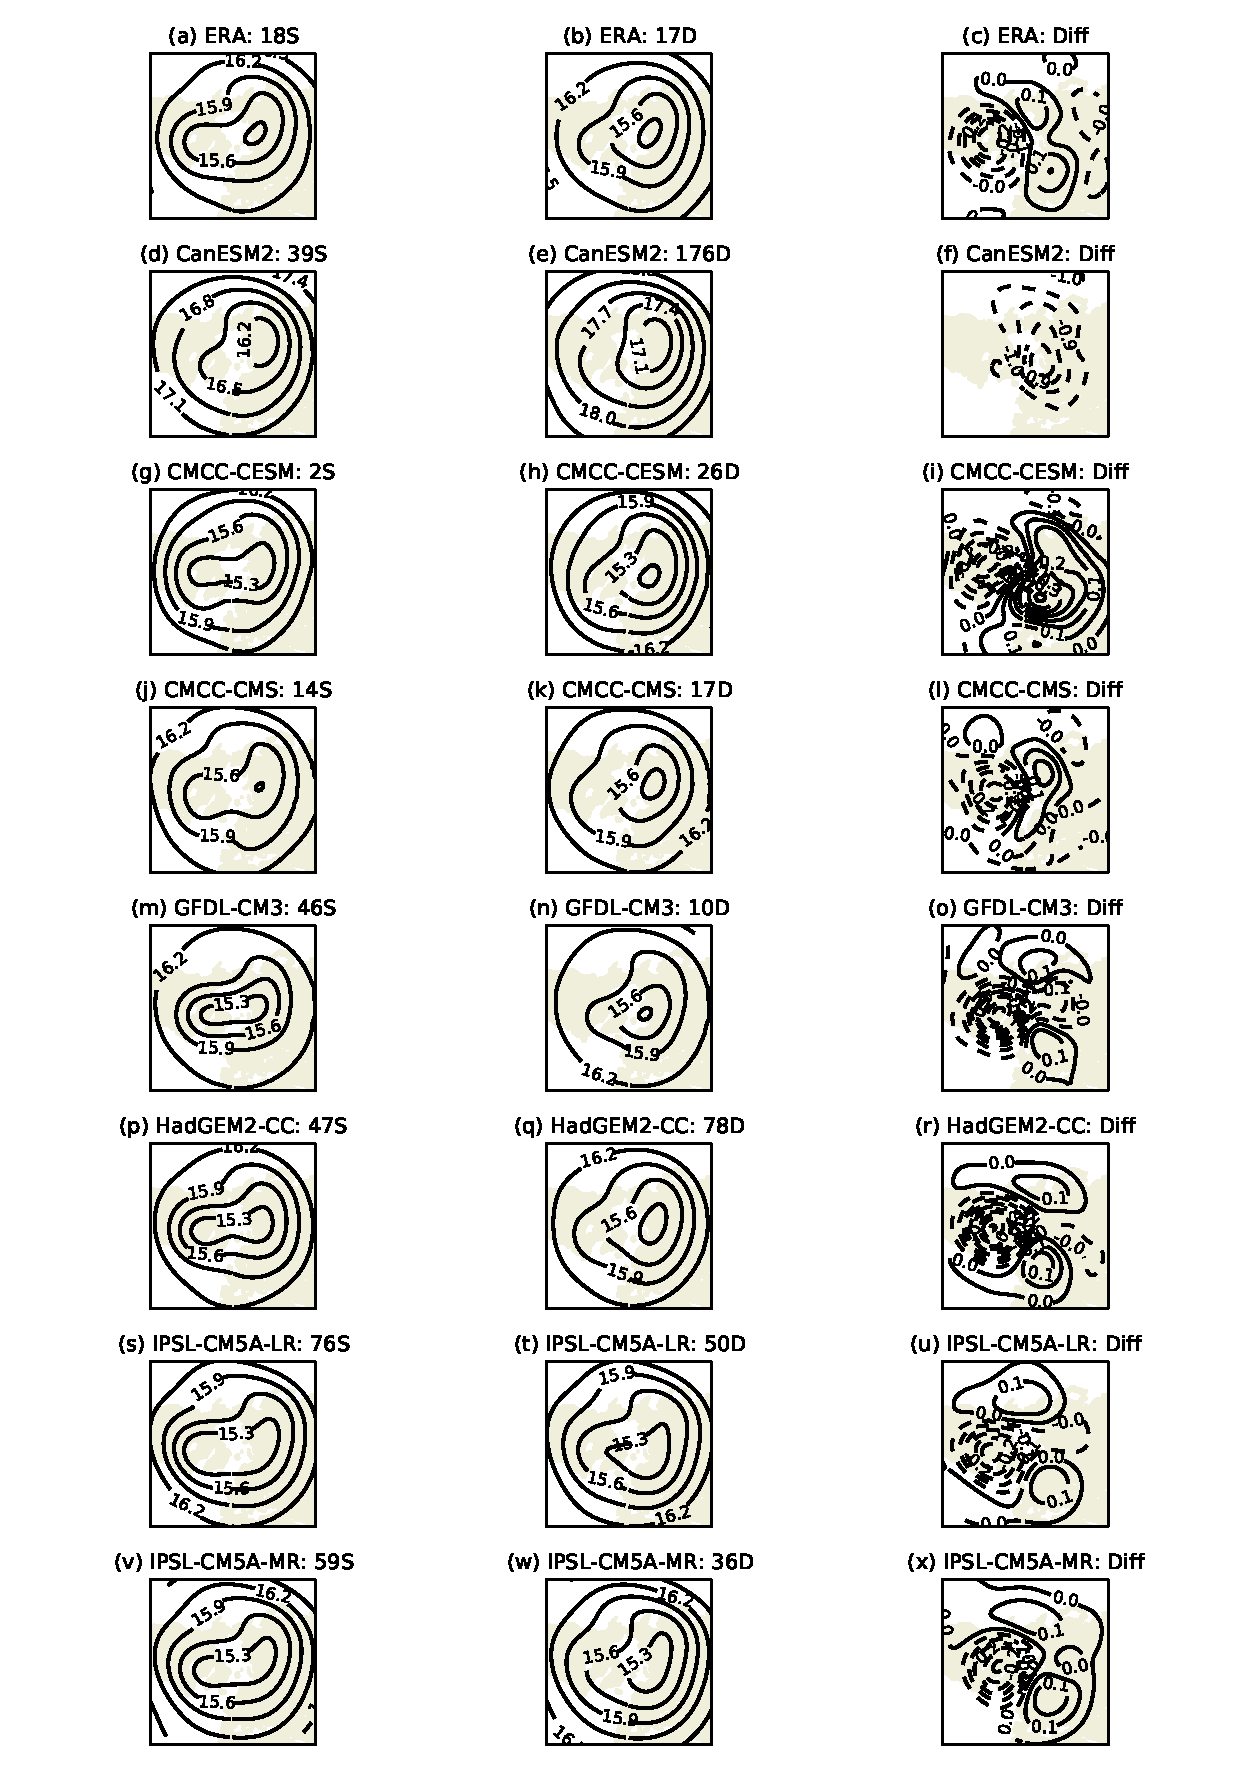
\includegraphics[width=\textwidth]{figures/chapter-models/100hPa_GPH1.pdf}
 \caption[NAM composites for splits and displacements in the CMIP5
 models]{Composites of 100~hPa geopotential height (km) averaged in the 10 days
   following the onset of split (S) and displaced (D) vortex events in ERA, each
   of the CMIP5 models, and the multi-model mean (MMM). The right hand column
   displays the difference of splits minus displacements. The multi-model mean
   is calculated so as to give each event an equal weighting.}
 \label{fig:cmip5_100hPa_comp}
\end{figure}

\begin{figure}
 \ContinuedFloat
 \centering
 \noindent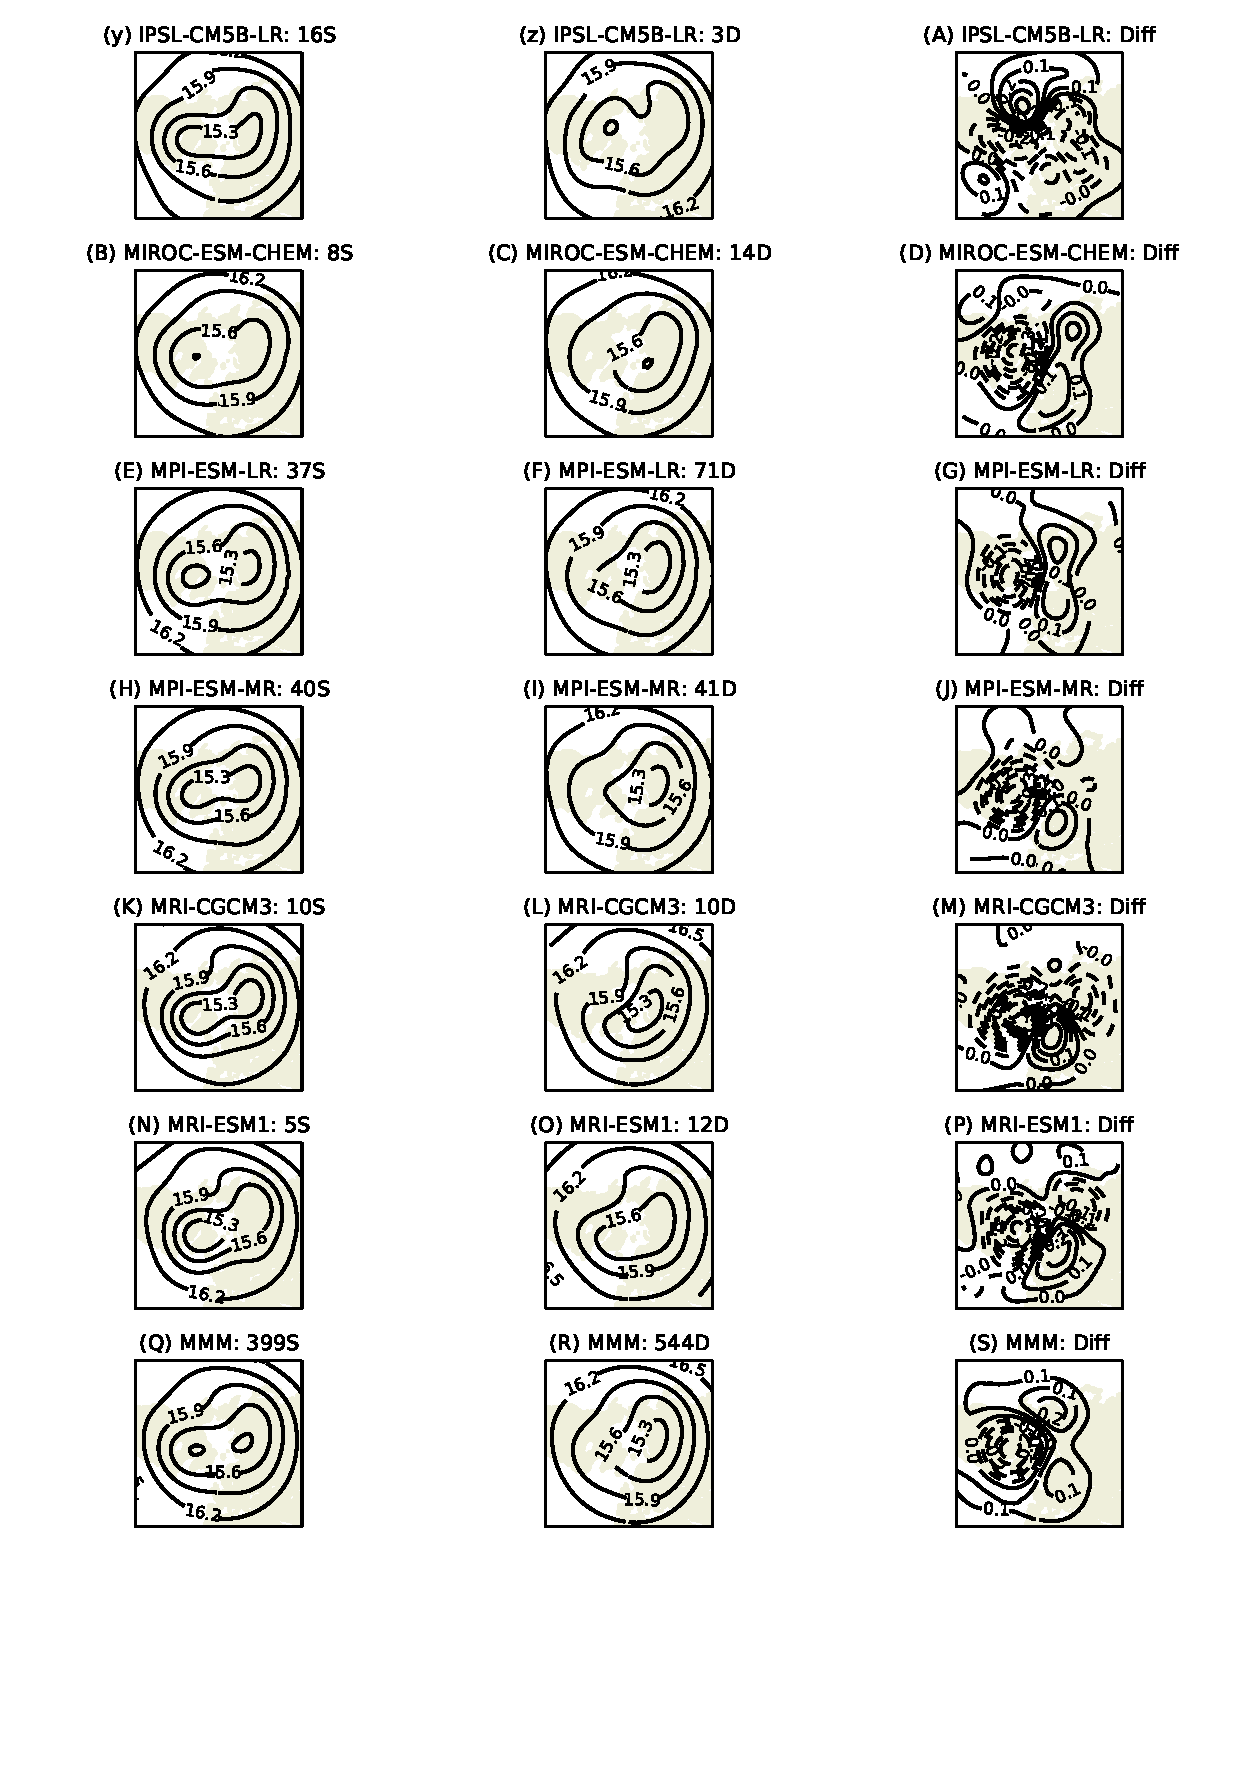
\includegraphics[width=\textwidth]{figures/chapter-models/100hPa_GPH2.pdf}
 \caption[]{(Continued)}
\end{figure}


\bigskip Figure \ref{fig:cmip5_mslp_diff} shows the split minus displaced vortex
composite difference for MSLP averaged 0-30 days following onset and the 100~hPa
$Z$ composite difference averaged 0-10 days following onset, for both ERA and
the CMIP5 MMM. Statistical significance in the MSLP difference is calculated by
a two-tailed bootstrap test with the null hypothesis that the anomalies
following split and displaced vortex events are populations from the same
probability distribution. The following procedure is used:
\begin{enumerate}
\item All events are grouped together and selected from them, with replacement,
  are two random subsets which are equal in size to the total number of split
  and displaced vortex events respectively.
\item The difference of the averages of these two subsets is taken.
\item The above is repeated 5000 times to form a distribution of random
  composite differences.
\item If the actual composite difference lies lower than the 2.5\% or higher
  than the 97.5\% levels of this distribution then it can be said there is a
  less than 95\% chance that an anomaly at least this large would arise if
  anomalies following split and displaced vortex events are populations from the
  same distribution. Hence the null hypothesis can be rejected.
\end{enumerate}
For the case of ERA, very little statistical significance in the
composite difference is seen, while in the CMIP5 MMM there are large
statistically significant regions. This is due to the greatly increased sample
size in CMIP5; a total of 943 events compared to just 35 in ERA. 

In the CMIP5 MMM difference the largest feature is the large positive anomaly (a
result of a more negative anomaly following displaced vortex events) over
Scandinavia, Eastern Europe and Russia. There is also a significant negative
anomaly over northern Canada and a positive anomaly in the western
Atlantic. This pattern is zonally asymmetric and so does not project strongly
onto the polar cap average, therefore explaining the small difference in polar
cap averaged $Z$ (Figure \ref{fig:cmip5_dripping_paint} (C,D)). The CMIP5
difference pattern also does not strongly project onto the NAO as there is a
similarly negative NAO following both split and displaced vortex events (Figure
\ref{fig:cmip5_mslp_comp} (C,D)). For the ERA MSLP difference there are stronger
negative anomalies over Europe (although not statistically significant) and
positive anomalies over the North Pole, which does project more strongly onto
the NAO, as discussed in Section \ref{sec:moments_analysis}. 

The CMIP5 difference of Figure \ref{fig:cmip5_mslp_diff} shows the positive
100~hPa $Z$ anomalies over Siberia over-lie the positive MSLP anomalies, while
the negative 100~hPa $Z$ over northern Canada over-lies negative MSLP
anomalies. A somewhat similar, but not statistically significant pattern is seen
in ERA, although the Siberian anomaly is more polewards and the negative anomaly
over Canada is much weaker. Importantly, the 100~hPa pressure surface lies
close to the tropopause, and 100~hPa $Z$ can therefore give an indication of
tropopause height. Indeed, comparing the 100~hPa $Z$ and tropopause height
anomalies for ERA (Figures \ref{fig:cmip5_100hPa_comp} (a,b) and
\ref{fig:tropopause_height} (c,d)) shows that anomalous negative $Z$ is
approximately co-located with an anomalously high tropopause, although the
tropopause height field is much noisier. 



\begin{figure}
 \centering
 \noindent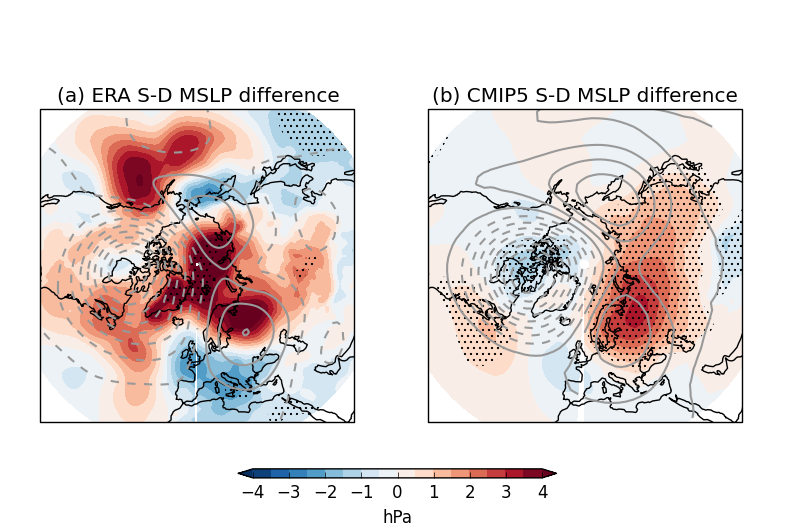
\includegraphics[width=\textwidth]{figures/chapter-models/mslp_diff.png}
 \caption[Difference of MSLP following split and displaced vortex
 events.]{Difference (S-D) of composites of mean sea-level pressure averaged
   0-30 days following split (S) and displaced (D) vortex events in ERA and the
   CMIP5 ensemble. Stippling indicates regions that are $>$95\% significant
   according to a two-tailed bootstrap test. Grey contours represent the
   difference in 100~hPa geopotential height averaged 0-10 days following events
   the contour interval is 40~m, dashed contours represent negative values and
   the lowest magnitude contours are $\pm$20~m. }
 \label{fig:cmip5_mslp_diff}
\end{figure}





\section{Discussion}
\subsection{Effect of model resolution}


\begin{figure}
 \centering
 \noindent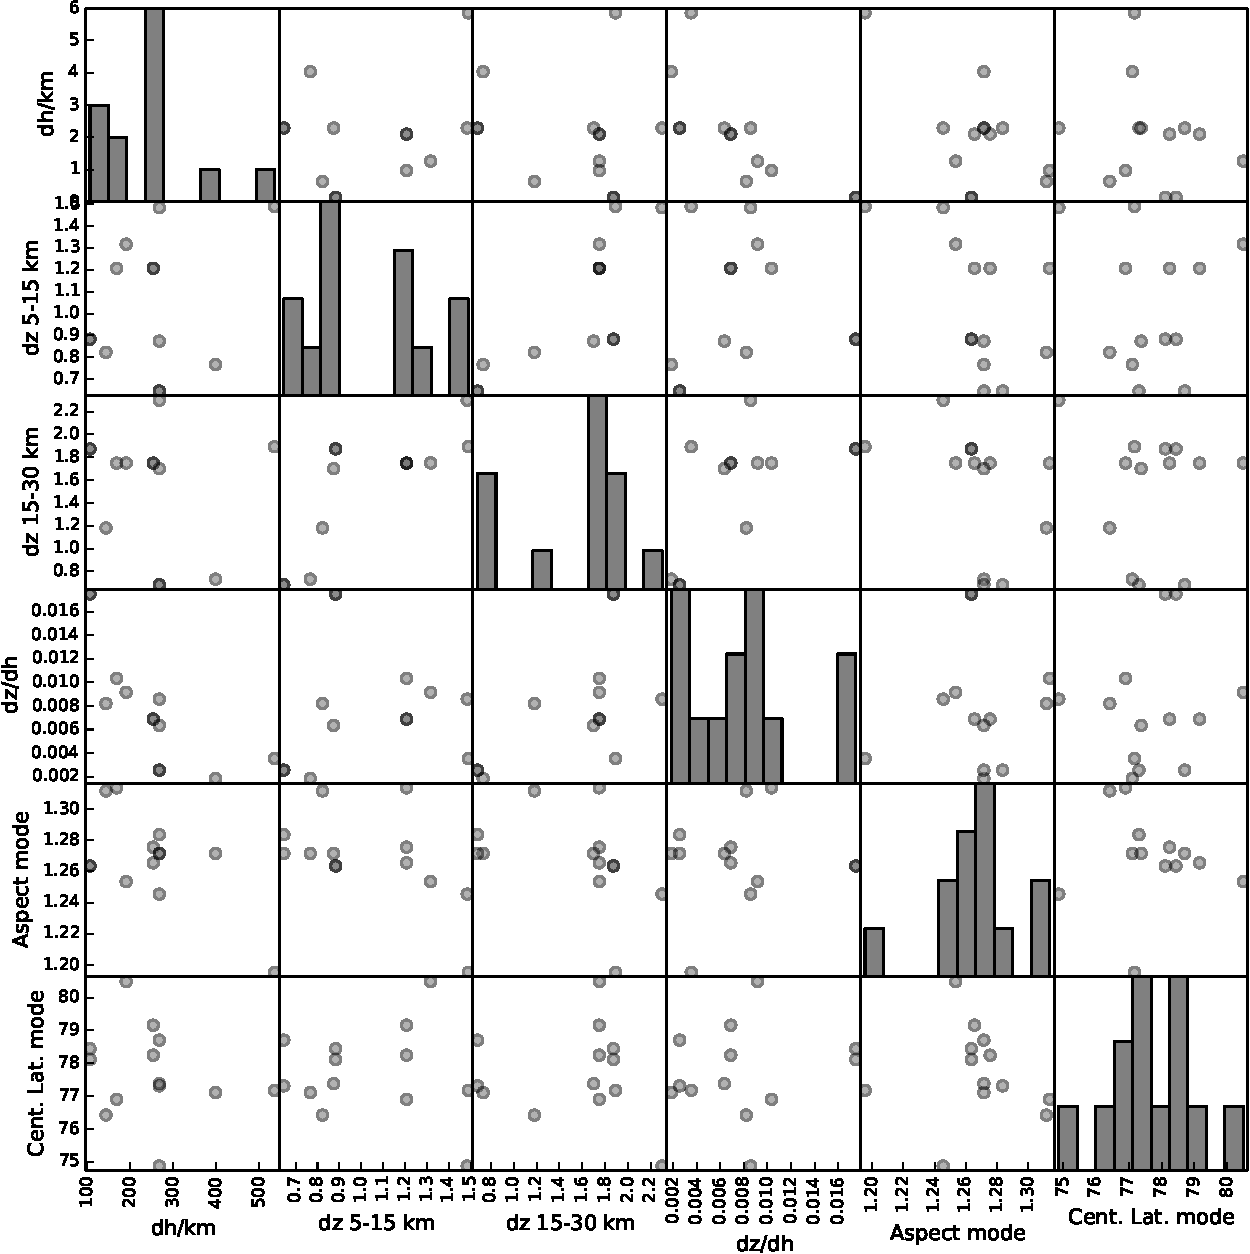
\includegraphics[width=\textwidth]{figures/chapter-models/scatter_matrix.pdf}
 \caption[Relationship between model resolution and moment diagnostics in the
 CMIP5 models.]{Relationship between model resolution, moment diagnostics, and
   stratosphere-troposphere coupling in the CMIP5 models. Model resolution is
   shown as horizontal resolution ($\mathrm{d}h$), vertical resolution
   ($\mathrm{d}z$) over 5-15~km and 15-30~km, and aspect ratio
   ($\mathrm{d}z$(5-15~km)$ / \mathrm{d}h$). Histograms for the relevant
   quantities are shown along the leading diagonal.}
 \label{fig:scatter_matrix}
\end{figure}

We have demonstrated that there are large differences in the representation of
the average undisturbed state of the stratospheric polar vortex among high-top
CMIP5 models. This amounts to an inter-model range in the modal centroid
latitude of more that 5$^{\circ}$ and in the aspect ratio of 0.12, which
corresponds to (77\% and 22\% of the ERA standard deviation
respectively). Because a similar number of models have a poleward as an
equatorward centroid latitude bias, the multi-model mean is approximately
accurate. In contrast, only two of 14 models have higher modal aspect ratio than
reanalysis.

Importantly, we have shown that these biases in the undisturbed state of the
vortex are closely related to biases in the frequency of split and displaced
vortex events. As a corollary, models therefore have a realistic representation
of variability relative to the average state. In order to understand the origin
of these biases we now consider whether any of the model horizontal and vertical
resolution properties listed in Table \ref{tab:models} are related to models'
polar vortex climatology. Figure \ref{fig:scatter_matrix} shows the correlations
between model resolution and modal aspect ratio and centroid latitude.

There are no statistically significant correlations between the modal aspect
ratio or centroid latitude and horizontal resolution or between the centroid
latitude and vertical resolution. However, a stronger relationship is found
between vertical resolution and the modal aspect ratio and this is shown in more
detail in Figure \ref{fig:aspect_vert_res}. The relatively wide scatter of
points as well as the small correlation coefficient values indicate that
vertical resolution fails to account for a substantial fraction of inter-model
variability in the modal aspect ratio. However, the $p$-values shown indicate a
relatively high level of statistical significance for both correlations. It
should be noted that these correlations are not highly influenced by
outliers. This can be seen by the bootstrap test $p$-values, as well as the rank
correlations which are $-0.60$ (96.9\%) and $-0.75$ (99.7\%) for vertical
resolutions over 5-15~km and 15-30~km respectively.

The two measures of vertical resolution, $\mathrm{d}z$ (5-15~km) and
$\mathrm{d}z$ (15-30~km), are themselves correlated (see Figure
\ref{fig:scatter_matrix}), so it is difficult to interpret which region (if any)
has the largest impact on the modal aspect ratio. It is interesting to note,
however, that \citet{Anstey2013} found vertical resolution among CMIP5 models to
correlate with increased NH winter blocking frequency. They found the strongest
relationship to be with upper-troposphere/lower-stratosphere (UTLS) vertical
resolution, which is where we find the strongest correlation with modal aspect
ratio (although slightly lower statistical significance; see Figure
\ref{fig:aspect_vert_res}). Blocking events are known to be closely linked to
stratospheric variability; they influence upwards wave propagation into the
stratosphere \citep{Polvani2004,Woollings2010c}, and may also be affected by
downwards the propagation of stratospheric anomalies
\citep{Tomassini2012,Mitchell2013,Vial2013}. Hence, the combination of the
present study with \citet{Anstey2013} may suggest that UTLS vertical resolution
is an important factor in the representation of stratosphere-troposphere
coupling.

Two important caveats should be noted in interpreting these correlations. First,
comparing pairs of models from the same family but with different resolutions
does not show a correlation between vertical resolution and modal aspect
ratio. In the present ensemble this comparison is limited to
IPSL-CM5A-LR/IPSL-CM5A-MR and MPI-ESM-LR/MPI-ESM-MR. It can be seen from Figure
\ref{fig:aspect_vert_res}(a) that the IPSL models have the same vertical
resolution but different modal aspect ratios and the MPI models have different
vertical resolutions but very similar modal aspect ratios. A similar effect is
also seen in comparing vertical resolution and blocking frequency
\citep{Anstey2013}. While this is a very limited comparison of only two pairs of
models, it may suggest that it is in fact other model differences which may give
rise to the correlations shown in Figure \ref{fig:aspect_vert_res}.

A second caveat is that interpreting this significance, it should be noted that
six different relationships between model resolution parameters and moment
diagnostics have been tested in Figure \ref{fig:scatter_matrix} (treating the
measures of vertical resolution as a single parameter since they are highly
correlated). Assuming these parameters to be independent (i.e. a binomial
distribution), there is an approximately 26\% chance of finding at least one
95\% significant correlation among those tested if the data are sampled from an
uncorrelated distribution. 

On the other hand, there is some physical motivation for the importance of UTLS
vertical resolution in the representation of stratosphere-troposphere coupling
because of the sensitivity of planetary wave propagation to vertical gradients
in this region. This sensitivity can be measured by the quasi-geostrophic
refractive index, $n_{s}$ \citep{Matsuno1970}, with planetary waves tending to
propagate towards regions of high $n_{s}$ and becoming evanescent in regions
where $n_{s}<0$. It is given by
\begin{equation}
  n_{s}^{2} = \frac{\overline{q}_{\phi}}{a\overline{u}} -
  \frac{s^{2}}{a^{2}\mathrm{cos}^{2}\phi} - \frac{f^{2}}{4N^{2}H^{2}} \, ,
\label{eq:refractive_index}
\end{equation}
where $N^{2}$ is the static stability, $H$ scale height, $s$ wavenumber, and
\begin{equation}
  \overline{q}_{\phi} = 2\Omega\mathrm{cos}\phi - \left[
    \frac{(\overline{u}\mathrm{cos}\phi)_{\phi}}{a\mathrm{cos}\phi} \right]_{\phi} -
  \frac{a}{\rho_{0}}\left(\frac{\rho_{0}f^{2}}{N^{2}}\overline{u}_{z}\right)_{z}
  \, .
\end{equation}
It is therefore apparent that $n_{s}$ is sensitive both to the vertical
gradient in static stability and the vertical shear of zonal wind. Using a
linear primitive equation numerical model, \citet{Chen1992} found a large
vertical gradient in static stability near the tropopause as well as a strong
vertical shear of the zonal flow. They found that small changes in these
quantities have a large effect on $n_{s}$, and therefore that the tropopause
acts as a ``valve'' for the propagation of planetary waves between the
troposphere and stratosphere. In a more recent observational study,
\citet{Grise2010} have confirmed the existence of fine-scale structure in static
stability near the tropopause. It therefore may be the case that a higher model
vertical resolution near the tropopause is necessary to capture this structure
and hence more accurately represent planetary wave propagation from troposphere
to stratosphere. 

The fact that there is not a significant relationship between the modal centroid
latitude and vertical resolution may suggest that wave-2 propagation is more
sensitive to vertical resolution than wave-1. This is because aspect ratio is
highly correlated with wave-2 activity and centroid latitude with wave-1
\citep{Waugh1999}. It might be expected that wave-2 propagation is more
sensitive to near-tropopause resolution because the `window' for permissible
wave-2 propagation is narrower (\citet{Charney1961}; Equation ??). Hence
smaller differences in vertical gradients are required to exclude wave-2
propagation than wave-1 propagation.

Overall, a more systematic study is necessary to understand the importance of
UTLS vertical resolution in the representation of stratosphere-troposphere
coupling by climate models. This should consist of a `clean comparison' of
models in which only vertical resolution is varied, and which therefore avoids
the difficulty of interpreting results when many parameters are varied at once
as in the CMIP5 ensemble.


% Z 500hPa


\begin{figure}
 \centering
 \noindent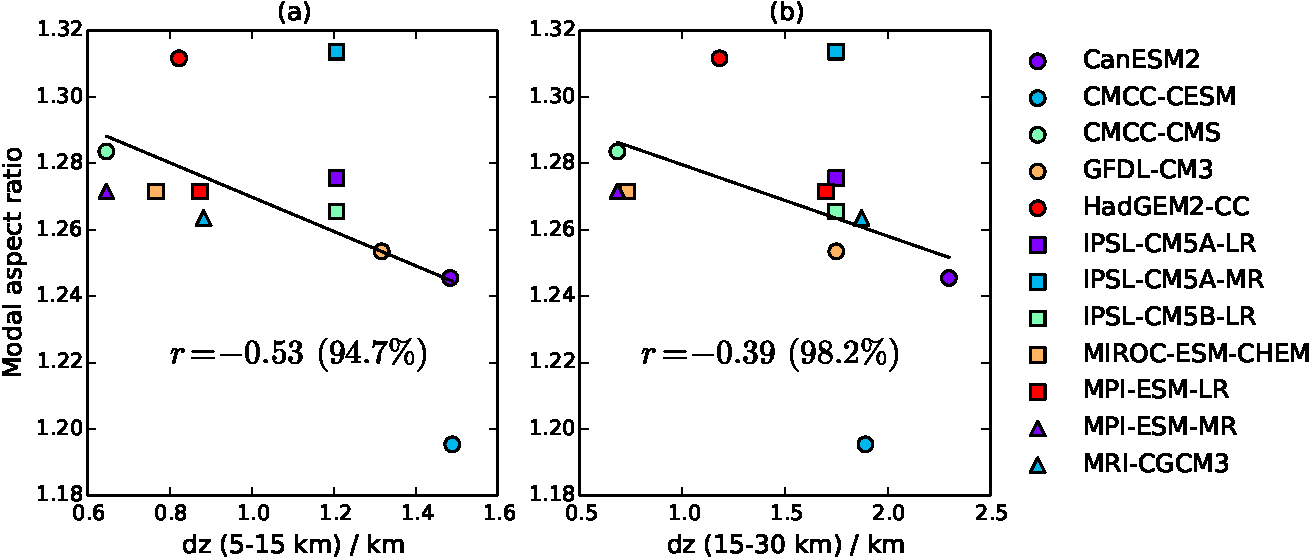
\includegraphics[width=\textwidth]{figures/chapter-models/aspect_ratio_resolution.pdf}
 \caption[Vertical resolution and modal aspect ratio.]{Expansion from Figure
   \ref{fig:scatter_matrix} of the correlation between modal aspect ratio and
   model vertical resolution over two regions (5-15~km and
   15-30~km). Correlations, $r$, are shown along with the $p$-value calculated by a
   bootstrap test with null hypothesis $r=0$.}
 \label{fig:aspect_vert_res}
\end{figure}


\subsection{Measures of stratosphere-troposphere coupling}

We have shown that zonally-averaged quantities such as polar cap $Z$ (which is
highly correlated with the NAM) following split and displaced vortex events are
much less consistent among models than the NAO. This inconsistency is dominated
by differences in the North Pacific, with some models showing positive MSLP
anomalies and others negative.

Following \citet{Baldwin2001a}, many studies of stratosphere-troposphere
coupling have focused on the lag-height behaviour the NAM. For instance the
comparison of stratosphere-troposphere coupling in high-top and low-top CMIP5
models by \citet{Charlton-Perez2013}. This and several other studies make
further approximations as to the zonal nature of the coupling by calculating the
NAM based on zonal-mean geopotential height, according to the method of
\citet{Baldwin2009}. Our results suggest that because of the difference in model
consistency over the two ocean basins, zonal-mean diagnostics or the NAM alone
are not a good descriptors of inter-model variability. Therefore, we suggest
that the NAO index or the full two-dimensional surface fields should be shown
alongside the NAM when making inter-model comparisons.

This difference between the NAM and NAO signals in CMIP5 models may also give
some insight into the physical relevance of these two modes of variability. Some
studies have suggested that the NAO is in fact a regional manifestation of the
planetary-scale annular structure of the NAM \citep[e.g.,][]{Thompson1998,
  Wallace2002}. Furthermore, many observational studies have asserted that
tropospheric anomalies following SSWs represent the NAM
\citep[e.g.,][]{Baldwin1999,Baldwin2001a,Thompson2000}. 

On the other hand, \citet{Ambaum2001} suggested that the NAO paradigm is a more
physically relevant measure of NH variability than the NAM. They found that MSLP
anomalies over the North Atlantic and Pacific are not significantly correlated
and argued that that the annular NAM pattern is a statistical
artifact. \citet{Huth2006} also showed that principal component analysis favours
the NAO as the more physically relevant mode of variability. Furthermore,
\citet{Ambaum2002} found that changes in North Pacific tropospheric subtropical
and polar jets are much less correlated with the strength of the stratospheric
polar vortex than are the North Atlantic jets.

Under the significant assumption that the CMIP5 models can accurately represent
the physics underlying these modes of variability, our results tend to favour
the NAO rather than the NAM as the more physically relevant mode, at least in
terms of stratosphere-troposphere coupling. 


% Fluctuation-dissipation
%Discuss NAO vs NAM



\subsection{Difference between split and displaced vortex events}
\label{sec:cmip5_discuss_split_displ}

As well as the consistent NAO signal following split and displaced vortex
events, we have found that there are also some consistent differences in
anomalies following the two types of event. In particular, MSLP anomalies
following displaced vortex events are more negative over Scandinavia and Siberia
than following split vortex events. From the fact that these MSLP differences
are co-located with 100~hPa $Z$ (Figure \ref{fig:cmip5_mslp_diff}), which is in
turn related to tropopause height, it may be possible to gain some understanding
of the mechanism behind the difference in the surface response to split and
displaced vortex events. 

This co-location of surface anomalies and tropopause height is consistent with a
localised spinup/spindown caused by stretching/compression of the tropospheric
column. Changes in tropopause height are, in turn, caused by the bending of
isentropic surfaces towards PV anomalies resulting from the movement of the
stratospheric polar vortex. Such a mechanism was discussed by
\citet{Hartley1998}, \citet{Ambaum2002}, \citet{Black2002}, and in Section
\ref{sec:mechanisms}.

Other mechanisms that have been proposed for stratosphere-troposphere coupling
fail to account for these regional differences. For instance, the amplification
of intrinsic modes of variability \citep{Robinson1991} can only explain
differences which project onto these modes such as the NAO or NAM, unlike
observed difference. Stratosphere-troposphere coupling by the reflection of
planetary waves \citep{JudithPerlwitz2003,Shaw2010} also cannot explain the
observed difference since it  does not project onto the dominant tropospheric
planetary wave modes. 

This argument relates only to the mechanism underlying the \emph{difference}
between the surface responses to split and displaced vortex events, and not to
the overall responses. It is important to note that there are many similarities
in the responses, especially in the NAO region. All the mechanisms discussed in
Section ?? can be used to explain a stratospheric influence on the NAO, and
since they are not physically inconsistent with one another, it is possible that
a number may operate at the same time. 

Unfortunately, the small number of observed split and displaced vortex events
combined with large tropospheric noise means there is very little statistical
significance in the observed difference of MSLP anomalies (see Figure
\ref{fig:cmip5_mslp_diff}(a)). Hence it is not possible to compare our model and
observational results for this difference, and there remains the
possibility that CMIP5 models do not realistically represent the surface
responses to split and displaced vortex events. Therefore, it is possible that
stratosphere-troposphere coupling mechanisms in models are different to those in
the real world. 

\section{Conclusions}

Applying the method developed in Chapter \ref{cha:moments}, the climatology of
the stratospheric polar vortex and its coupling with the troposphere has been
analysed in stratosphere-resolving CMIP5 simulations. Returning to the three
main objectives of this chapter (Section \ref{sec:models_introduction}), the
following conclusions have been reached:
\begin{enumerate}

\item \textbf{How do models represent the stratospheric polar vortex and
    stratosphere-troposphere coupling?}

  A wide range of biases among CMIP5 models has been found in the average state
  of the stratospheric polar vortex. Some models have a vortex which is too
  equatorward, while others too poleward. The majority of models have a vortex
  which is too circularly symmetric. These biases have been shown to relate
  closely to biases in the frequency of split and displaced vortex events. In
  the multi-model mean, however, the frequency of these events is in agreement
  with observations. 

  Almost all models accurately simulate the more barotropic nature of split
  vortex events compared to displaced vortex events. MSLP anomalies following
  these events consistently show a negative NAO in line with observations, but
  are much less consistent in the North Pacific, leading to a large spread when
  zonal mean quantities are investigated.

\item \textbf{Is model resolution related to vortex variability?}

  There is a statistically significant correlation between near-tropopause
  vertical resolution and modal aspect ratio among models. However, this
  relationship is not seen among the two pairs of models from the same
  family. On the other hand, the tropopause region is known to be important for
  the propagation of planetary waves due to high vertical gradients of zonal
  wind shear and static stability. This may be suggestive of the need for high
  vertical resolution to accurately simulate stratospheric planetary wave
  activity and hence vortex aspect ratio. No relationships have been found
  between horizontal resolution and vortex variability.

\item \textbf{Can models be used to understand mechanisms behind
    stratosphere-troposphere coupling?}

  Consistent differences in the MSLP anomalies following split and displaced
  vortex events in the CMIP5 models have been found to be co-located with the
  difference in near-tropopause $Z$ anomalies. This is consistent with a
  localised tropospheric response to stretching or compression of the
  tropospheric column being the mechanism behind the different responses to the
  two events. It also excludes mechanisms which rely on projections onto major
  modes of variability such as the NAO or NAM. This result only applies to the
  difference between responses to split and displaced vortex events, not the
  individual responses, which share many similarities.
\end{enumerate}

% Re-address aims from introduction

%%% Local Variables:
%%% mode: latex
%%% TeX-master: "thesis"
%%% End:

\chapter{The role of the stratosphere in seasonal prediction}
\label{cha:seas}

\begin{quotation}
  Most of work in this chapter which relates to the Southern Hemisphere was
  published in \emph{Journal of Climate} \citep{Seviour2014}.
\end{quotation}


\section{Introduction}
\label{sec:seas-introduction}

Accurate prediction of the atmospheric circulation several months in advance
relies on the presence of low-frequency predictable signals in the climate
system. It has now been demonstrated that the stratosphere is an important
pathway for the communication of predictable tropical signals across the globe;
in particular, the El Ni\~no-Southern Oscillation (ENSO) \citep{Bell2009,
  Ineson2009, Hurwitz2011}, Quasi-Biennial Oscillation (QBO)
\citep{Marshall2009, Garfinkel2011}, and 11-year solar cycle \citep{Haigh2003,
  Gray2013}. These teleconnections allow for the possibility of significant
predictability in regions remote from the direct effect of the signal. Despite
this, many operational seasonal forecast models include only a poor
representation of the stratosphere \citep{Maycock2011}, and it has been
suggested that this contributes to their lack of seasonal forecast skill in the
extratropics \citep{Smith2012}.

Furthermore, because stratospheric anomalies persist for longer than those in
the troposphere and can influence surface weather patterns, the initial
conditions of the stratosphere itself can act as a source of enhanced
predictability \citep{Baldwin2003a, Charlton2003, Christiansen2005,
  Hardiman2011}. Because the effect of the stratosphere on the troposphere is
especially pronounced following SSW events, past work has focused on the
influence of these events on forecast skill. For instance, both
\citet{Kuroda2008} and \citet{Sigmond2013} found that enhanced tropospheric
predictability can be obtained if forecasts are initialised at the onset of SSW
events. However, SSWs are highly nonlinear events which previous studies have
not found predictable beyond about two weeks in advance
\citep{Marshall2010,Taguchi2014}. This may therefore limit their usefulness in
seasonal prediction. SSWs also occur almost exclusively in the NH, with only one
event in the approximately 60 year record having been observed in the SH, in
September 2002 \citep{Roscoe2005}.

As discussed in Section \ref{sec:strat-sudd-warm}, the rarity of SSWs in the SH
is a result of less dynamical forcing from vertically propagating planetary
waves in the SH relative to the NH stratosphere. This reduced dynamical forcing
also means that anomalies in the Antarctic stratosphere persist for longer than
those in the Arctic \citep{Simpson2011}. Hence, the SH stratospheric circulation
may be predictable on longer time scales, and thus more useful for seasonal
forecasts despite the lack of SSWs. Indeed, \citet{Thompson2005} and
\citet{Son2013a} have found that smaller-amplitude variations in the Antarctic
stratospheric polar vortex are followed by coherent temperature and pressure
anomalies at the Earth's surface which resemble the Southern Annular Mode (SAM)
pattern. These observations led \citet{Roff2011} to find that improved forecasts
of the SAM up to 30 days ahead may be achieved with a stratosphere-resolving
model. As the dominant mode of variability in the extratropical SH, the SAM
affects the position of storm tracks, rainfall, surface air temperature, and
ocean temperatures across the extratropics \citep[e.g.,][]{Silvestri2003,
  Reason2005, Hendon2007}. As such, there are considerable societal benefits and
interests in its prediction \citep{Lim2013}.

Another reason for interest in the prediction of the Antarctic stratosphere is
the interannual variability in springtime ozone depletion, which can
significantly affect the amount of harmful ultraviolet radiation reaching the
Earth's surface over the Southern Hemisphere. The magnitude of this interannual
variability is a significant fraction of the magnitude of long-term depletion
caused by emission of chlorofluorocarbons (CFCs) and other ozone-depleting
substances. While ozone-depleted air is confined over the polar region by the
stratospheric polar vortex during winter and spring (resulting in the ozone
hole), this air is released to mid-latitudes following the ultimate breakdown of
the vortex (final warming) in late spring/early summer. The extent of the
resulting summertime ozone depletion is largely determined by the total deficit
in ozone over the Antarctic during spring \citep{Bodeker2005}.

As discussed in Section \ref{sec:polar-strat-ozone}, dynamics play an important
role in ozone depletion. Indeed, \citet{Salby2012} have shown that interannual
variations in Antarctic ozone depletion are highly correlated with changes in
planetary wave forcing of the stratosphere. They found that the anomalous
vertical EP flux at 70~hPa poleward of 40$^{\circ}$S during August-September
explains almost all the interannual variance of anomalous ozone depletion during
September--November. Using this relationship, they postulate that accurate
prediction of planetary wave forcing could allow skillful seasonal forecasts of
ozone depletion.

% The influence of planetary wave forcing on ozone depletion comes about through
% both chemical and dynamical mechanisms. Planetary wave breaking causes an
% increase of the strength of the stratospheric residual mean meridional
% circulation \citep{Haynes1991}, with a resultant increase in large-scale descent
% and adiabatic warming over the pole. This warming inhibits the formation of
% polar stratospheric clouds which have a vital role in the activation of halogen
% species that cause the chemical depletion of ozone. The increased meridional
% circulation as well as an enhancement of horizontal two-way mixing caused by
% planetary wave breaking, also causes an increase in the dynamical transport of
% tropical ozone-rich air to the polar regions, further increasing ozone
% concentrations.  Breaking planetary waves can also modify the geometry of the
% stratospheric polar vortex, stripping away elements of ozone-depleted air
% \citep{Waugh1994}, or in the extreme case of the 2002 SSW causing the ozone hole
% to split in two \citep{Charlton2005a}.

In this chapter, we address directly the predictability of the stratospheric
polar vortices using a set of hindcasts (or historical re-forecasts) from a new
operational seasonal forecast system with a fully stratosphere-resolving general
circulation model. The system accurately simulates the climatology of the NH
stratospheric polar vortex including the aspect ratio and centroid
latitude. However, we find it does not skilfully predict the winter mean vortex
strength, the occurence of SSWs, or split and displaced vortex events. On the
other hand, we find significant skill in the prediction of the Antarctic
stratospheric polar vortex up to four months in advance, including for the 2002
SSW. Using the observed relationship between column ozone quantities and the
stratospheric circulation, we are then able to infer skillful predictions of
springtime ozone depletion, confirming the hypothesis of \citet{Salby2012}. This
exceeds the lead-time of other contemporary ozone forecasts, which are typically
no more than two weeks \citep{Eskes2005}. The forecast system also shows
significant levels of skill in the prediction of the surface SAM at seasonal
lead times. By studying the variation of hindcast skill with time and height, we
demonstrate that this skill is significantly influenced by the descent of
predictable stratospheric circulation anomalies.

\section{Seasonal forecast system}
\label{sec:seas-forec-syst}

The analysis in this chapter is based on results from a set of hindcast
predictions produced by the Met Office Global Seasonal Forecast System 5
(GloSea5) \citep{MacLachlan2014}. This system is based upon the HadGEM3 coupled
general circulation model \citep{Hewitt2011}, with an atmospheric resolution of
0.83$^{\circ}$ longitude by 0.56$^{\circ}$ latitude, 85 quasi-horizontal
atmospheric levels and an upper boundary at 85~km. The ocean resolution is
0.25$^{\circ}$ in longitude and latitude, with 75 quasi-horizontal levels.

Initial conditions for the atmosphere and land surface were taken from the
ERA-Interim reanalysis \citep{Dee2011}, and initial ocean and sea-ice
concentrations from the GloSea5 Ocean and Sea Ice Analysis, based on the FOAM
data assimilation system \citep{Blockley2013}. The ERA-Interim data are linearly
interpolated onto model levels between the surface and 64.56~km (near 0.1~hPa),
and the 64.56~km values are then replicated onto the four subsequent levels up
to 85~km. FOAM data are on the same grid as the ocean model. Beyond
initialisation the model takes no further observational data, and contains no
flux corrections or relaxations to climatology. The model lacks interactive
chemistry and ozone concentrations are fixed to observed climatological values
averaged over 1994--2005, including a seasonal cycle from the
Stratosphere-troposphere Processes and their Role in Climate (SPARC) climatology
\citep{Cionni2011}. Climate forcings such as CO$_2$ and CH$_4$ concentrations
are set to observed values up to 2005 and then follow the IPCC RCP4.5 scenario. 

\citet{Scaife2013} have shown that this seasonal forecast system produces highly
skillful forecasts of the North Atlantic Oscillation (NAO) during the Northern
Hemisphere winter. They found the correlation of the ensemble mean DJF average
NAO with observed values to be $r=0.62$, which is statistically significant from
zero at the 99\% level. They argue that the combined effects of ENSO, QBO and
sea-ice teleconnections, as well as the increased ocean resolution which has
improved the representation of Northern Hemisphere blocking events
\citep{Scaife2011a}, contribute to this skill.

Hindcast accuracy is verified by comparison to the ERA-Interim reanalysis
\citep{Dee2011}. As discussed in Chapter \ref{cha:moments}, the ERA-Interim data
set has been demonstrated to have realistic representation of the stratospheric
meridional circulation \citep{Seviour2012, Monge-Sanz2013}. It also assimilates
observations of ozone concentrations, and this assimilation has been
demonstrated to be in close agreement with independent satellite data
\citep{Dragani2011}

In this chapter, hindcasts are anaysed for two seasons; December--February (DJF)
for prediction of the Northern Hemisphere winter stratospheric polar vortex, and
September--November (SON) for the Southern Hemisphere. The SON season is chosen
because it represents the time of maximum SH ozone depletion and stratospheric
polar vortex variability. For SON a 15-member ensemble of hindcasts was run for
each year in the period 1996--2009, while for the DJF analysis a longer
24-member ensemble is available for the winters 1992/1993--2011/2012. The
hindcast length is approximately four months from three separate start dates
spaced two weeks apart and centered on 1st August (SON) or 1st November (DJF),
with an equal number of members initialised on each start date. Members
initialised on the same start date differ only by stochastic parameterisation of
model physics, using the Stochastic Kinetic Energy Backscatter v2
\citep[SKEB;][]{Bowler2009} scheme. Details of the hindcast runs for these two
seasons are summarised in Table \ref{tab:seas_runs}.
\begin{table}[h]
\centering
\begin{tabular}{llll} \hline
  Season & Hindcast period                & Initialisation dates & Ensemble size
  \\ \hline
  DJF    & 92/93--11/12 (20 years) & 25/10, 01/11, 09/11  & 24 (8 on each date) \\
  SON    & 1996--2009 (14 years)           & 25/07, 01/08, 09/08  & 15 (5 on each
                                                                   date) \\ \hline
\end{tabular}
\caption{Summary table of the two sets of hindcast simulations analysed.}
\label{tab:seas_runs}
\end{table}

It should be noted that the 20-year, 20-member ensemble hindcasts of DJF were
extended from a 14-year, 15-member ensemble, the same as as the SON
hindcasts. These extended simulations are, however, slightly shorter than the
original ensemble; ending at the beginning of March rather than the beginning of
April. This therefore limits our analysis of the full ensemble so as not to
include March. Furthermore, some variables were not produced by the extended DJF
ensemble and so the original sorter ensemble must be used in some cases, which
is made clear in the text where necessary.

\begin{figure}[p] \vspace*{-3cm} \centering
   \noindent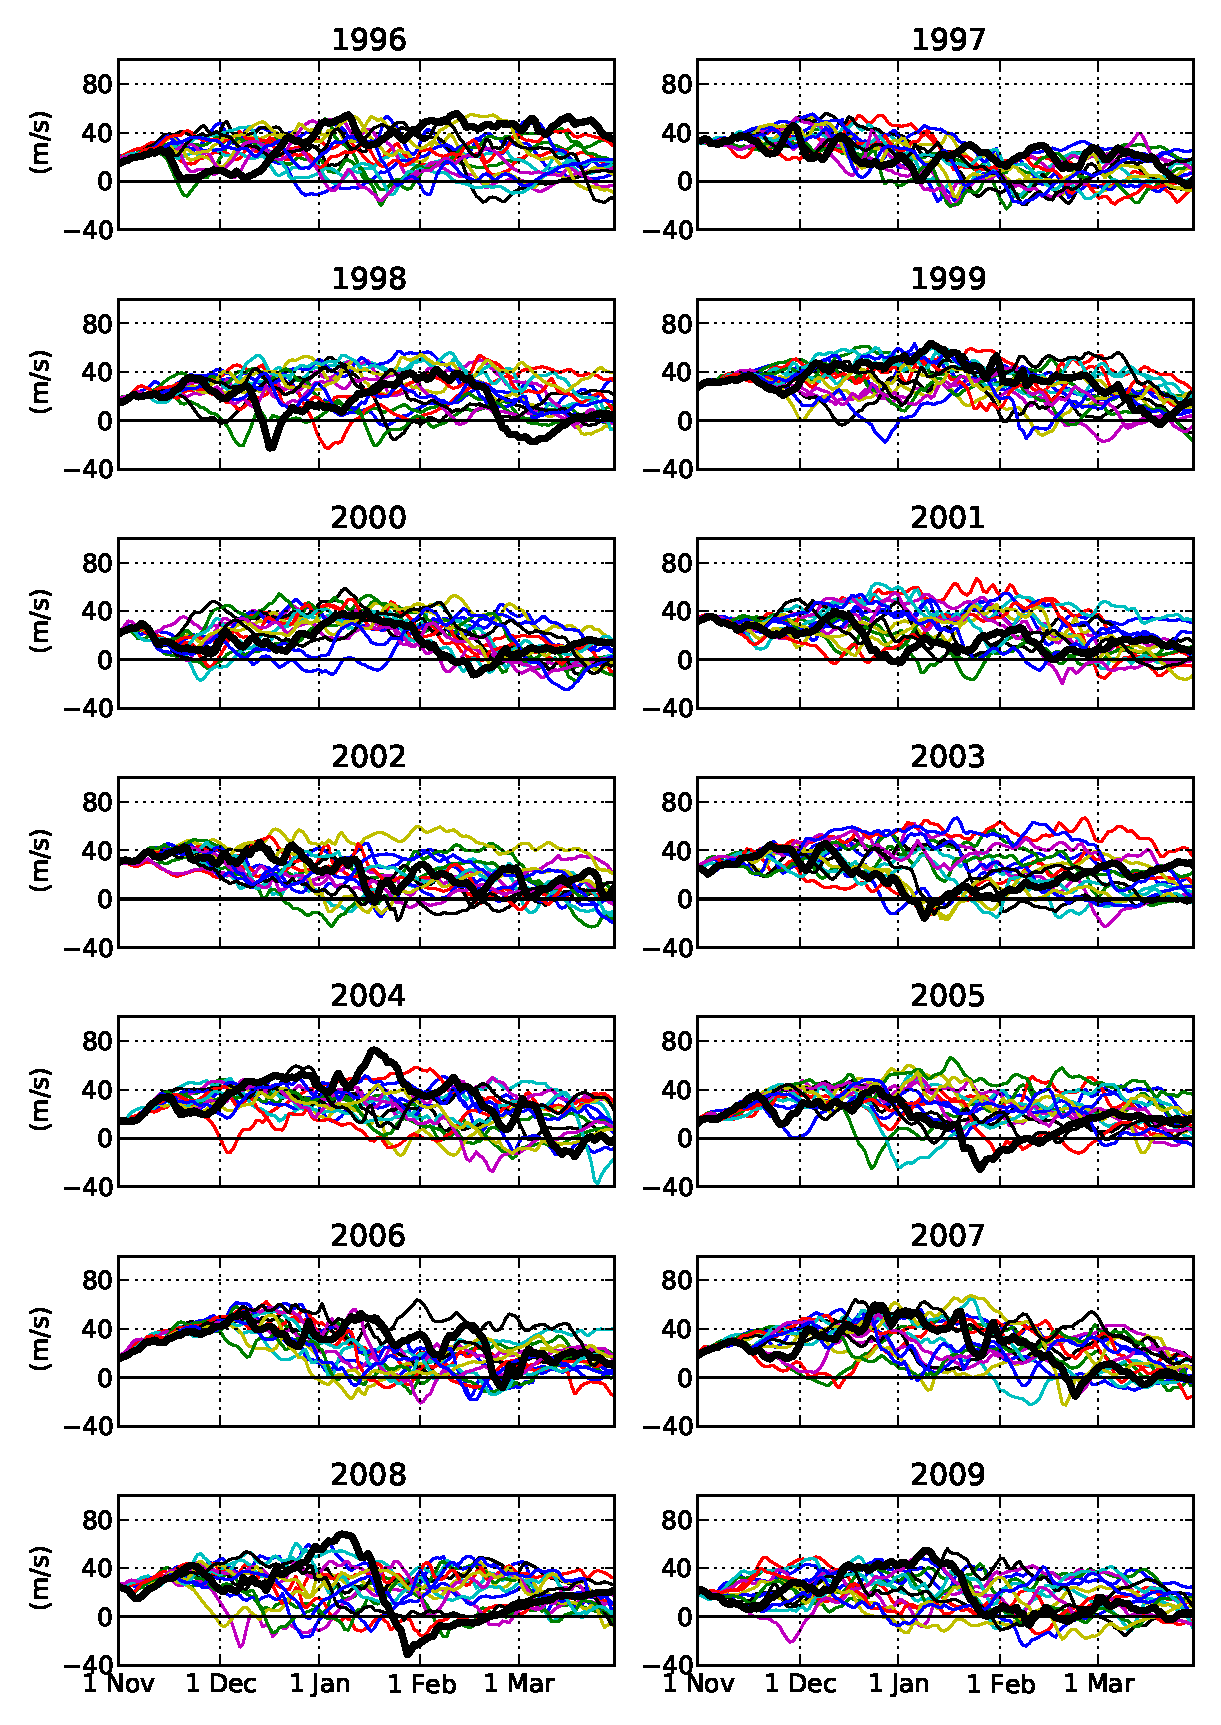
\includegraphics[width=\textwidth]{figures/chapter-seasonal/zm_winds_nh_poststamp.pdf}
   \caption[Timeseries of $\overline{u}$ at 60$^{\circ}$N, 10~hPa, for all
   GloSea5 ensemble members.]{Timeseries of zonal-mean zonal wind in the Arctic
     polar vortex ($60^{\circ}$N, 10~hPa) in the ERA-Interim reanalysis (thick
     black lines) and the GloSea5 ensemble hindcasts (thin coloured
     lines). Individual ensemble members are initialised from dates centred on
     November 1st. Years refer to the year of the initialisation date.}
   \label{fig:nh_poststamp}
\end{figure}

\begin{figure}[p] \vspace*{-3cm} \centering
  \noindent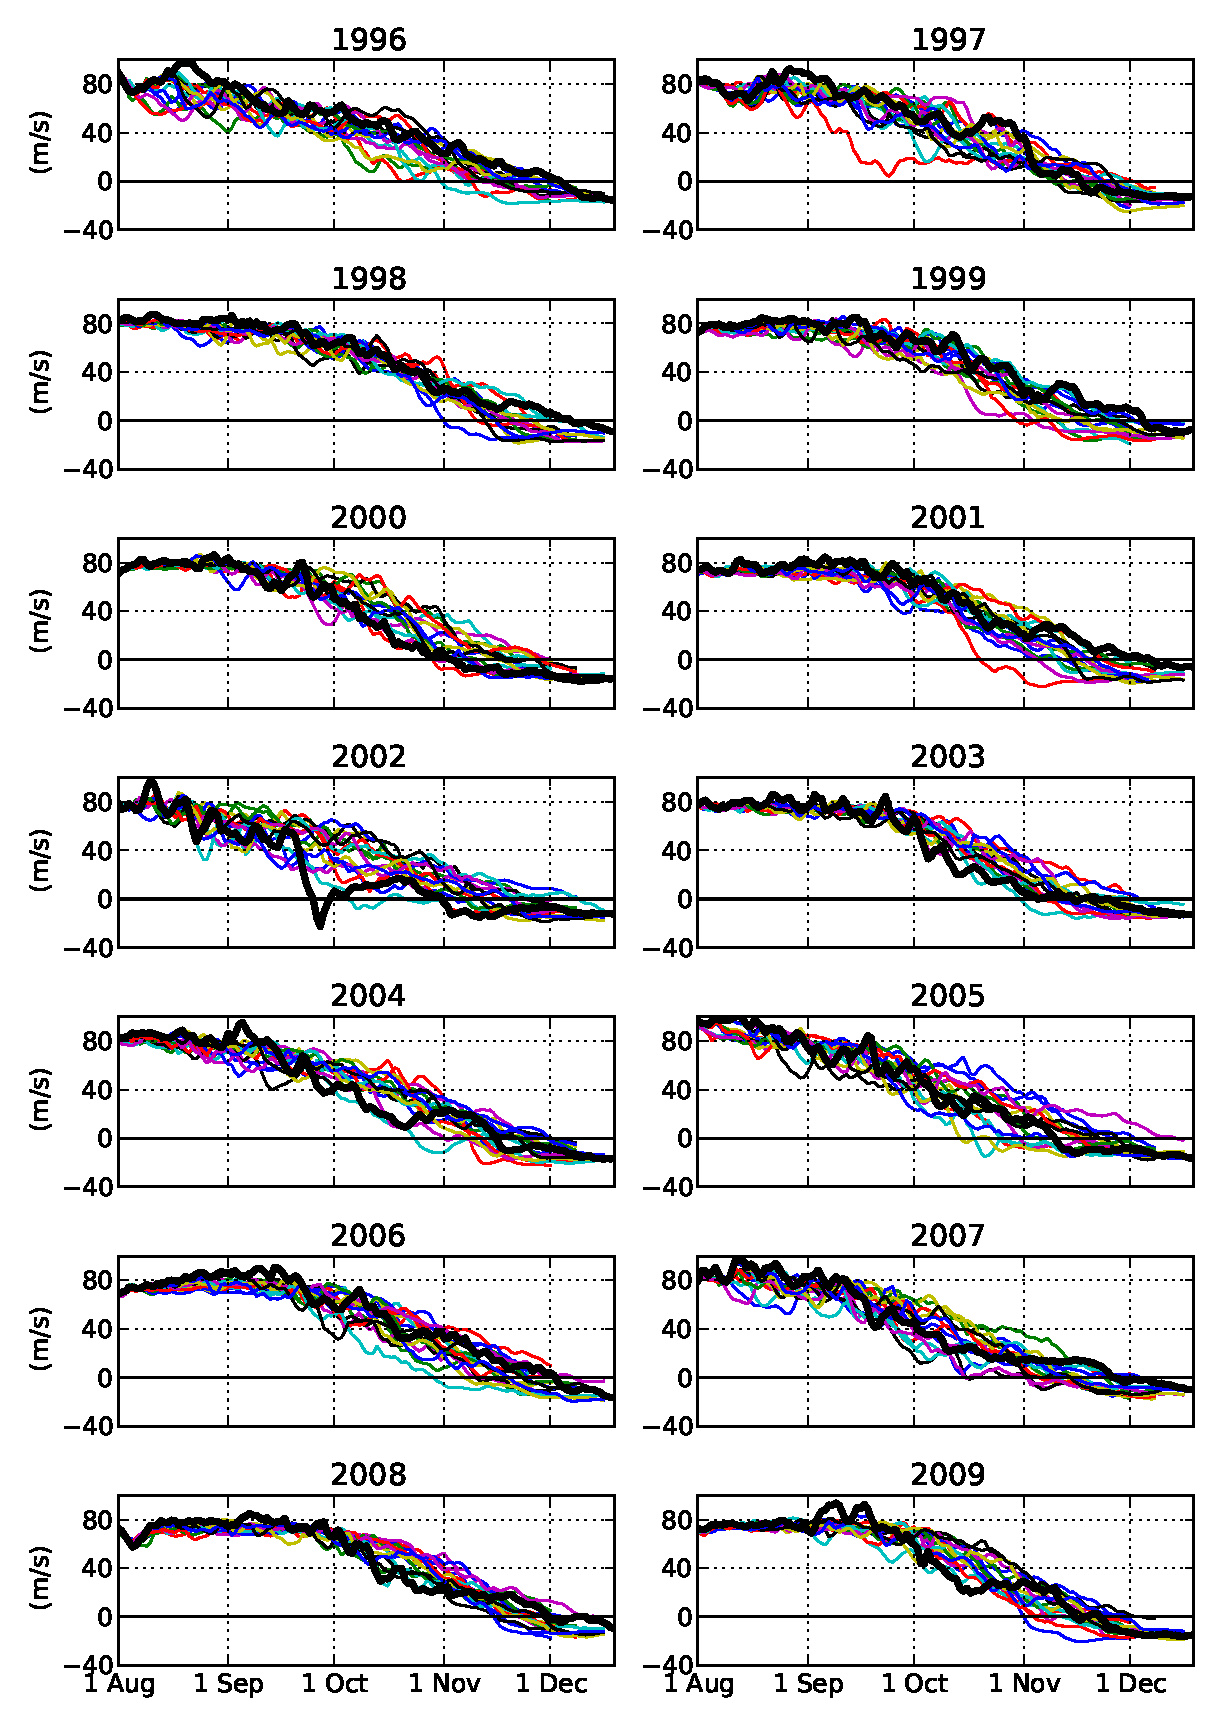
\includegraphics[width=\textwidth]{figures/chapter-seasonal/zm_winds_sh_poststamp.pdf}
  \caption[Timeseries of $\overline{u}$ at 60$^{\circ}$S, 10~hPa, for all
  GloSea5 ensemble members.]{As figure \ref{fig:nh_poststamp} but for the
    zonal-mean zonal wind in the Antarctic polar vortex ($60^{\circ}$S, 10~hPa),
    and ensemble members initialised from dates centred on August 1st.}
  \label{fig:sh_poststamp}
\end{figure}

In order to illustrate these hindcast simulations, timeseries of zonal-mean
zonal wind ($\overline{u}$) at 10~hPa are shown for $60^{\circ}$N from
November--March (Figure \ref{fig:nh_poststamp}) and $60^{\circ}$S from
August--December (Figure \ref{fig:sh_poststamp}). ERA-Interim values are also
shown in both cases (black lines). These are the approximate positions of the
centre of the mean position of the stratospheric polar vortex in the
mid-stratosphere, and therefore indicate the strength of the stratospheric polar
vortex. In order to make the figures comparable, the shorter 14-year, 15-member
ensemble is shown for the NH. It can immediately be seen that there is a much
greater ensemble spread in the NH, owing to the much greater dynamical
variability of the NH stratospheric polar vortex. In both cases it can also be
seen that the ensemble spread is initially small and increases rapidly after
approximately 15-30 days. This demonstrates the initial constraint to
ERA-Interim and the rapid growth of small differences in initial conditions,
because of the chaotic nature of the atmosphere. The predictive skill of for the
Northern Hemisphere (DJF) is analysed in the next section, and the Southern
Hemisphere (SON) in Section \ref{sec:south-hemisph-result}.


\section{Northern Hemisphere results}
\label{sec:north-hemisph-result}
% NH data
% 8.5 events/decade - 3.5 splits, 5.0 displs 
% min 47% (01/02) max 100% (97/98) (any event in winter)

The climatology of Arctic stratospheric polar vortex winds in the GloSea5
hindcasts is compared to the ERA-Interim reanalysis climatology in Figure
\ref{fig:sh_zmzw_clim}. As in Figure \ref{fig:nh_poststamp}, the strength of the
stratospheric polar vortex is measured by the zonal-mean zonal wind
($\overline{u}$) at 60$^{\circ}$N and 10~hPa. The composite for the GloSea5
hindcasts is formed from all the individual ensemble members over the winters
1992/1993--2011/2012 (a total of 480), while that from ERA-Interim is a
composite of the same 20 winters. It can be seen that the mean, interquartile
range and 95th percentile range of the GloSea5 values agree well with the
ERA-Interim values, although the ERA-Interim values are noisier as would be
expected from a sample size consisting of fewer years.

\begin{figure}[t]
  \noindent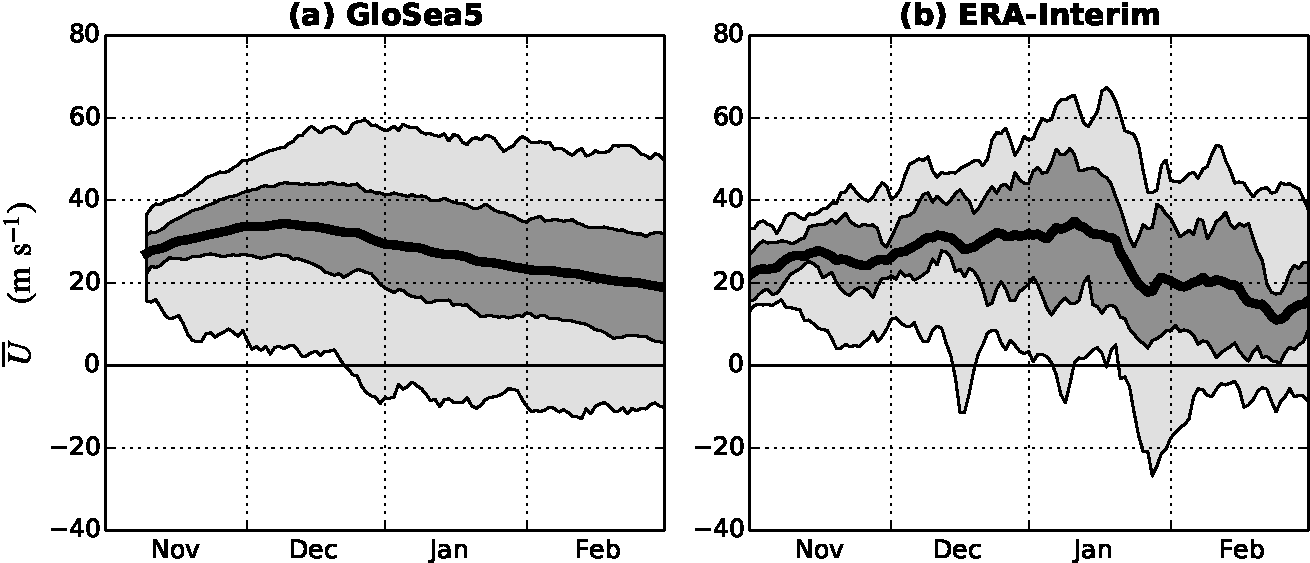
\includegraphics[width=\textwidth,angle=0]{figures/chapter-seasonal/zmzw_climatologies_nh.pdf}\\
  \caption[NH comparison of GloSea5 and ERA-Interim zonal-mean zonal wind
  climatologies.]{Time series of daily 10~hPa zonal-mean zonal wind
    ($\overline{u}$) at 60$^{\circ}$N for all GloSea5 ensemble members (a) and
    ERA-Interim (b) from 1992--2011. The thick black line indicates the mean,
    dark grey shading the interquartile range and light grey the 95th percentile
    range.}\label{fig:nh_zmzw_clim}
\end{figure}

Figure \ref{fig:nh_moments_glosea} shows the joint distribution of the apsect
ratio and centroid latitude moment diagnostics calculated over DJF from the
GloSea5 hindcasts, along with the equivalent values from ERA-Interim. These
diagnostics have been calculated from geopotential height following the method
described in Chapter \ref{cha:moments}. Both aspect ratio and centroid latitude
distributions closely match those of ERA-Interim, and the joint distribution
shows the characteristic triangular shape which is related to the occurrence of
split and displaced vortex events. Together, Figures \ref{fig:nh_zmzw_clim} and
\ref{fig:nh_moments_glosea} demonstrate that GloSea5 accurately simulates the
mean state and variability of the stratospheric polar vortex in the
mid-stratosphere.  

\begin{figure}[t] \centering
  \noindent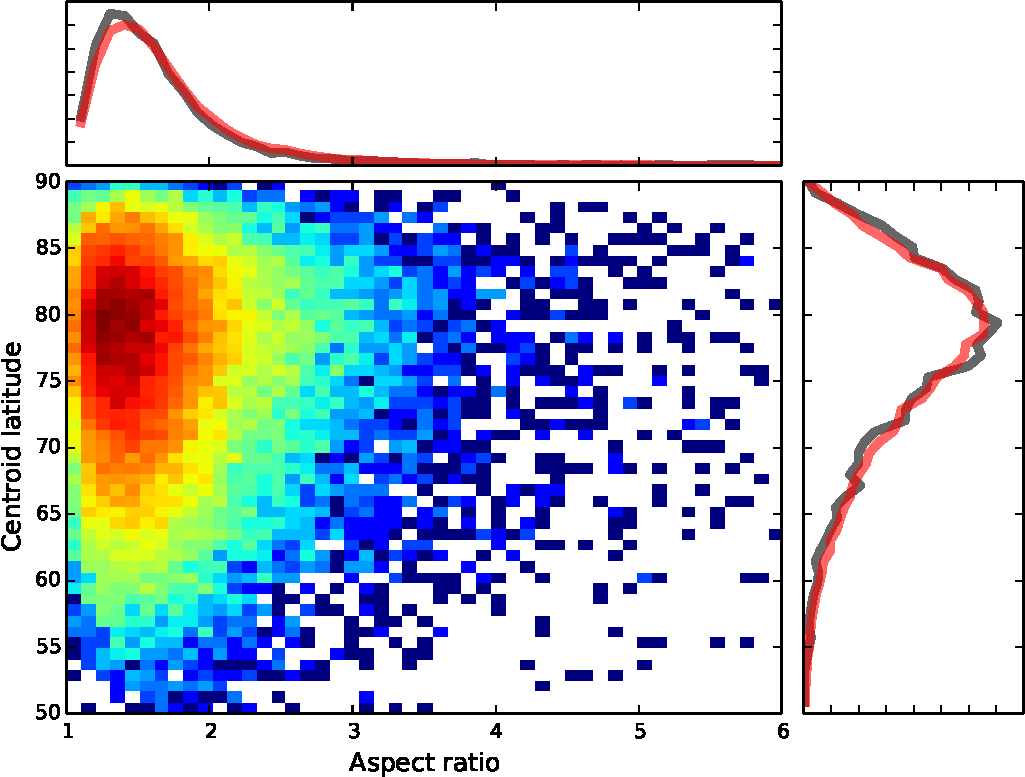
\includegraphics[width=0.7\textwidth,angle=0]{figures/chapter-seasonal/GloSea_moments_histogram.pdf}\\
  \caption[Moment diagnostics for GloSea5.]{Distribution (see Figure
    \ref{fig:cmip5_moments_stats}) of the centroid latitude and aspect ratio
    diagnostics derived from geopotential height for all GloSea5 ensemble
    members (red lines) and ERA-Interim (grey lines) over 1992--2011. The joint
    distribution is plotted with a logarithmic colour scale such that red
    represents the densest regions.}\label{fig:nh_moments_glosea}
\end{figure}

The GloSea5 hindcast predictions of interannual variability of the NH
stratospheric polar vortex winds are shown in Figure
\ref{fig:nh_zmzw_timeseries}. Anomalies are defined from the relevant
climatology of either GloSea5 or ERA-Interim. For GloSea5, this climatology is
calculated from the mean of each day across all ensemble members in all years,
while for ERA-Interim the climatology is the mean of each day, smoothed with a
30-day running mean (in order to account for its increased noise due to the
reduced sample size). Results are shown for DJF averages, corresponding to a 1
month average lead time. The correlation between the GloSea5 ensemble mean and
ERA-Interim is $r=0.24$ which is not statistically significant at the 95\% level
(under the null hypthesis that the two timeseries are
uncorrelated). Significance is calculated using a two-tailed bootstrap test,
whereby the percentile of the observed correlation is calculated from the
distribution of correlations of a large number ($\sim 10~000$) of pairs of time
series formed by re-sampling with replacement from the original time series. As
elswhere in this thesis, these significance tests are used because they make
fewer assumptions about the underlying structure of the data than parametric
tests \citep{Wilks}.

\begin{figure}[t]
  \noindent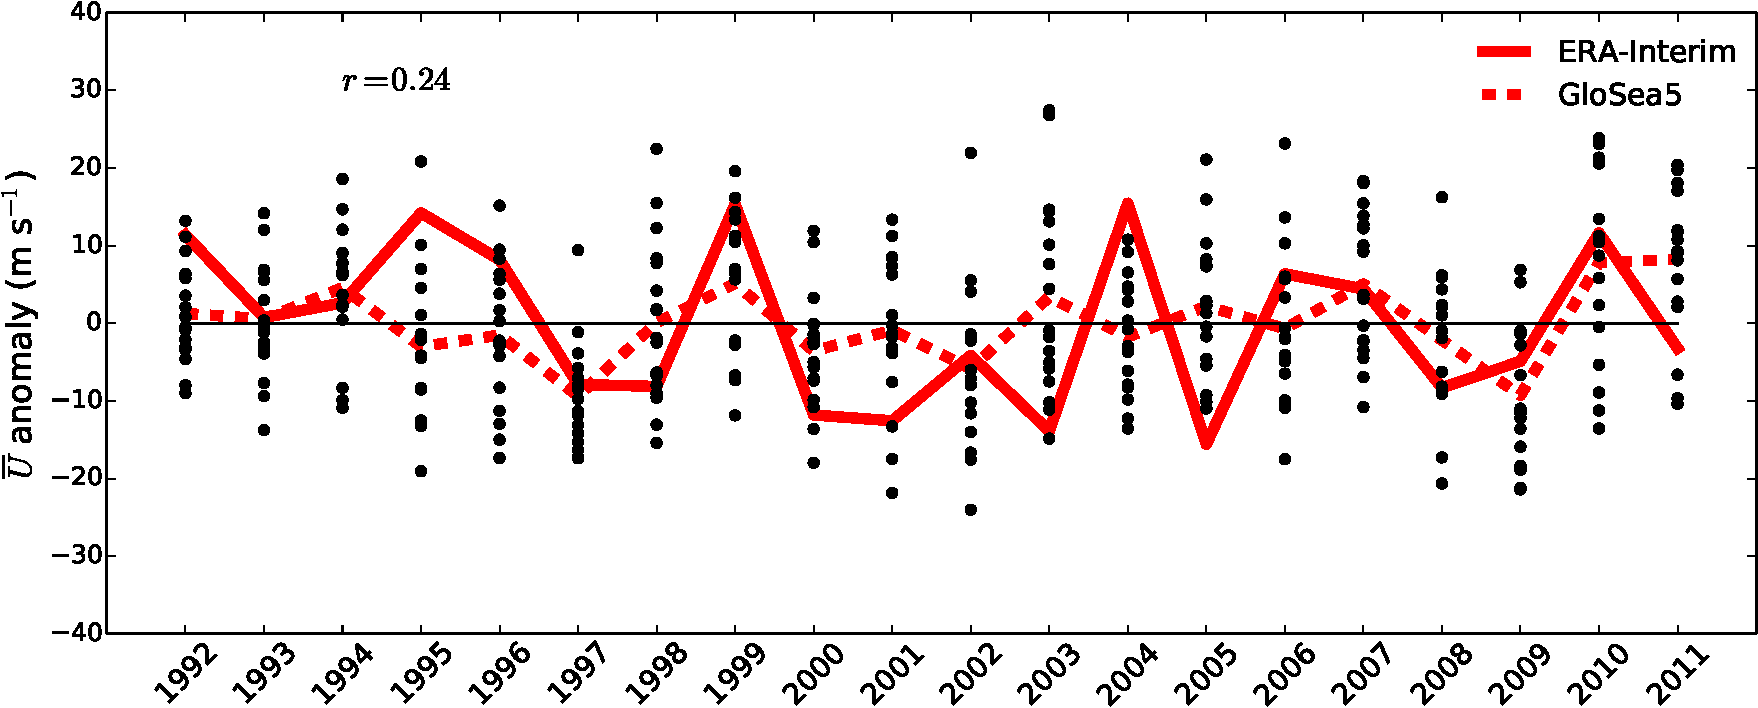
\includegraphics[width=\textwidth,angle=0]{figures/chapter-seasonal/DJF_ZMZW_NH.pdf}\\
  \caption[DJF $\overline{u}$ anomalies for GloSea5.]{DJF mean anomalies of
    $\overline{u}$ at $60^{\circ}$N and 10~hPa for the GloSea5 ensemble mean and
    ERA-Interim. Black dots represent individual ensemble members. The
    correlation between the GloSea5 ensemble mean and ERA-Interim is $r=0.24$,
    which is not statistically significant from zero. Years refer to the year of
    the initialisation date.}\label{fig:nh_zmzw_timeseries}
\end{figure}

Although no significant skill is found in the prediction of the seasonal mean
strength of the stratospheric polar vortex, it might nonetheless be the case
that skilful predictions of SSW events can be made. This is assessed using
receiver operating characteristic (ROC) curves, a standard method in forecast
evaluation, particularly of binary events \citep[e.g.,][]{Wilks}. In order to
calculate the ROC curve, the following procedure is followed:
\begin{enumerate}[1.]
\item For each ensemble member in each year, determine whether an SSW occurs
  (winters with one SSW and two SSWs are treated the same). 
\item Select a threshold for the prediction of an SSW (e.g., 60\% of ensemble
  members forecast an SSW). 
\item For the given threshold determine the fraction of years for which a SSW
  was correctly predicted (``hit rate'') and the fraction for which a SSW was
  predicted but none occurred (``false alarm rate''). 
\item Repeat the steps 2-3 for a range of thresholds from 0-100\%.
\end{enumerate}
In a skilful system the ROC curve should indicate a higher hit rate than false
alarm rate, bending towards the upper left corner of the graph, while a random
forecast will pass along the 1-1 line. 

\begin{figure}[t] \centering
  \noindent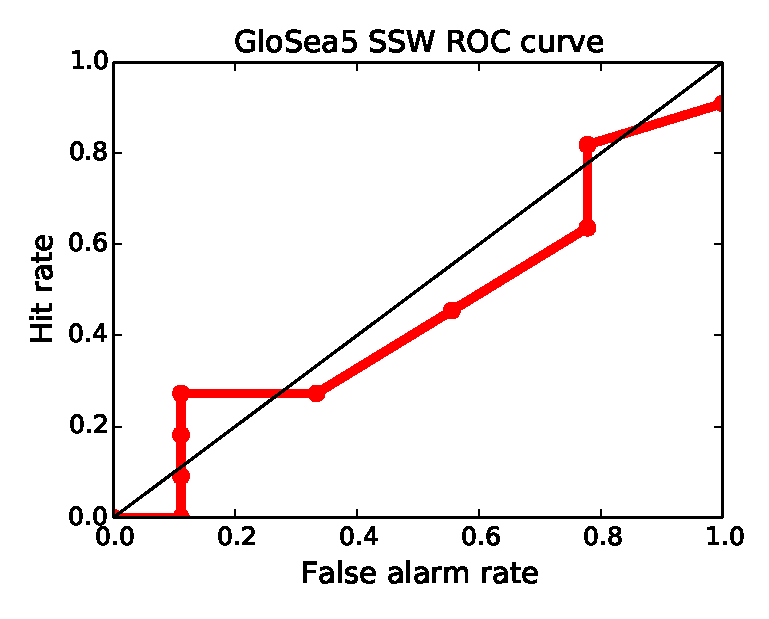
\includegraphics[width=0.7\textwidth,angle=0]{figures/chapter-seasonal/SSW_ROC.pdf}\\
  \caption[ROC curve for the prediction of SSWs.]{Receiver operating
    characteristic (ROC) curve for the prediction of SSW events during DJF for
    1992--2011. SSWs are defined as a reversal to easterly $\overline{u}$ at
    60$^{\circ}$N 10~hPa, and must be separated by at least 30
    days.}\label{fig:ssw_roc}
\end{figure}

Figure \ref{fig:ssw_roc} shows the ROC curve for SSWs during DJF, determined by
the traditional reversal of $\overline{u}$ at 60$^\circ$N 10~hPa, with the
additional criterion that events must be separated by at least 30 days. It can
be seen that the calculated ROC curve lies close to the 1-1 line indicating
little skill in these predictions. This is despite quite large variations in the
fraction of ensemble members predicting SSWS; from 47\% (winter 2001/2002) to
100\% (winter 1997/1998). 

\begin{figure}[t] \centering
  \noindent\includegraphics[width=\textwidth,angle=0]{figures/chapter-seasonal/glosea_split_displ_ROC_any.pdf}\\
  \caption[ROC curves for the prediction of split and displaced vortex
  events.]{Receiver operating characteristic (ROC) curves for the prediction of
    split (a) and displaced (b) vortex events in all GloSea5 ensemble members
    over 1992--2011. Split and displaced vortex events are identified from
    geopotential height-derived moment diagnostics using the method described in
    Chapter \ref{cha:moments}.}\label{fig:split_displ_roc}
\end{figure}

A similar analysis for the prediction of split and displaced vortex events is
shown in Figure \ref{fig:split_displ_roc}. These events have been calculated
from the geopotential height-derived moment diagnostics, using the same
procedure as decribed in Chapter \ref{cha:moments}. Again, little skill can be
seen in the predictions of these events, with both ROC curves lying close to the
1-1 line. It should be noted that GloSea5 predicts a high frequency of split and
displaced vortex events (8.5 events/decade; 3.5 split, 5.0 displaced), compared
to the observed value of 7 events/decade. This is perhaps not surprising given
the HadGEM3 model used in GloSea5 is of the same family as HadGEM2-CC, which was
found to have the highest frequency of events in Chapter \ref{cha:models}.

\begin{figure}[t] \centering
  \noindent\includegraphics[width=\textwidth,angle=0]{figures/chapter-seasonal/NH_lag_height_corr.pdf}\\
  \caption[Lag-height correlation of NH polar cap geopotential
  height.]{Correlation of GloSea5 ensemble mean polar cap (60-90$^{\circ}$N)
    geopotential height anomalies ($Z'$) with ERA-Interim values from
    1996--2009, as a function of time and height. All values are smoothed with a
    30-day running mean before correlations are calculated. The contour interval
    is 0.1 and all colored regions are greater than zero at the 95\% confidence
    interval, using a bootstrap test at each time at height. The blue dashed
    line indicates the approximate polar cap mean tropopause level
    \citep{Wilcox2012}.}\label{fig:nh_pc_gph_corr}
\end{figure}

\bigskip The evolution of NH hindcast skill as a function of lag and height is
evaluated in Figure \ref{fig:nh_pc_gph_corr}. This shows the correlation of
ERA-Interm and GloSea5 ensemble mean polar cap (60-90$^\circ$N) average
geopotential height anomalies ($Z'$; which is highly correlated with the NAM
\citep{Kushner2010}). Values of $Z'$ are smoothed with a 30-day running mean
before correlations are calculated, and plotted such that values for the 15th
December represent the correlation of the ERA-Interim and GloSea5 ensemble mean
December mean values (without this smoothing, a noisier but similar pattern of
correlations is seen). Geopotential height data on several levels in the
stratosphere is only available in the shorter 14-year, 15-member ensemble, and
so the analysis in this figure is limited to these data. Between 1st-9th
November the ensemble mean is taken as the average of the 10 initialised
ensemble members, and the average of all 15 ensemble members is used after this
date.

In mid-November, significant correlations are seen in Figure
\ref{fig:nh_pc_gph_corr} in both the stratosphere and troposphere, as would be
expected from the initialisation of the hindcasts from ERA-Interim data (skill
is seen to rapidly decay in the tropopause region, however). This skill persists
for longer in the stratosphere than the troposphere, owing to the longer
timescales of stratospheric variability \citep[e.g.,][]{Simpson2011}, however,
by mid-December no significant correlations are seen in the stratosphere or
troposphere. 

Significant correlations return in the troposphere in late Janurary/February,
and to a lesser extent in the stratosphere. This result is similar to that for
the NAO prediction in the same system, which has a greater skill in February
than January (Adam Scaife, Met Office Hadley Centre, personal communication,
2013). A possible explanation for this behaviour is due to the influence of
ENSO, which has been determined to have the greatest effect on the NH
extratropics during late Janurary and February \citep{Bell2009}. If indeed the
influence of ENSO is important, it is not clear whether this arises from a
tropospheric or stratospheric pathway, although the fact that tropospheric skill
is greater than stratospheric may suggest the tropospheric pathway is more
important.

Detailed analysis of the mechanisms behind the NH surface skill is beyond the
scope of this chapter which investigates the role of the stratosphere. Because
skill in the prediction of the NH stratosphere has been demonstrated to be low,
attention is now turned to the SH. However, the implications of these results
are discussed further in Section \ref{sec:seas-discussion}. 


\section{Southern Hemisphere results}
\label{sec:south-hemisph-result}

\subsection{Stratospheric polar vortex}


The climatology of Antarctic stratospheric polar vortex winds in the GloSea5
hindcasts is compared to the ERA-Interim reanalysis climatology in Figure
\ref{fig:sh_zmzw_clim}. The strength of the stratospheric polar vortex is
measured by the zonal-mean zonal wind ($\overline{u}$) at 60$^{\circ}$S and
10~hPa, which is approximately the center of the mean position of the vortex in
the mid-stratosphere. The composite for the GloSea5 hindcasts is formed from all
the individual ensemble members over 1996--2009 (a total of 210), while that
from ERA-Interim is a composite of all years from 1979--2010 (a total of 32
years). It can be seen that the mean of the GloSea5 hindcasts agrees very
closely with ERA-Interim throughout the spring, with only a slight bias towards
weaker winds in August and September. The interquartile and 95th percentile
ranges of GloSea5 and ERA-Interim also agree well, although the ERA-Interim
values are noisier as would be expected from a sample size consisting of fewer
years.

\begin{figure}[t]
  \noindent\includegraphics[width=\textwidth,angle=0]{figures/chapter-seasonal/zmzw_climatologies_crop.pdf}\\
  \caption[Comparison of GloSea5 and ERA-Interim zonal-mean zonal wind
  climatologies.]{Time series of daily 10~hPa zonal-mean zonal wind
    ($\overline{u}$) at 60$^{\circ}$S for all GloSea5 ensemble members from
    1996--2009 (a) and ERA-Interim from 1979--2010 (b). The thick black line
    indicates the mean, dark gray shading the interquartile range and light gray
    the 95th percentile range. Individual time series of the ensemble member of
    GloSea5 for 2002 which simulated an SSW, and 1997 which simulated a
    near-SSW, and the year with an observed SSW (2002) are shown in
    red.}\label{fig:sh_zmzw_clim}
\end{figure}

The GloSea5 hindcast predictions of interannual variability of the Antarctic
stratospheric polar vortex winds are shown in Figure
\ref{fig:zmzw_ozone}(a). Anomalies are defined from the relevant climatology of
either GloSea5 or ERA-Interim. For GloSea5, this climatology is calculated from
the mean of each day across all ensemble members in all years, while for
ERA-Interim the climatology is the mean of each day, smoothed with a 30-day
running mean (in order to account for its increased noise due to the reduced
sample size). Results are shown for September--November (SON) averages,
corresponding to a 1 month average lead time. The correlation between the
GloSea5 ensemble mean and ERA-Interim is 0.73, which is statistically
significant from zero at the 99\% confidence level, and has a 95\% confidence
interval of (0.37,0.90). This correlation does not depend strongly on particular
years; the correlation remains significant at the 95\% level ($r=0.57$) if the
year 2002 (which has the greatest anomaly) is excluded. Significance is
calculated using a two-tailed bootstrap test, whereby the percentile of the
observed correlation is calculated from the distribution of correlations of a
large number ($\sim 10,000$) of pairs of time series formed by re-sampling with
replacement from the original time series. These significance tests make fewer
assumptions about the underlying structure of the data than parametric tests
\citep{Wilks}, and are used throughout this study.

\begin{figure}[t]
  \noindent\includegraphics[width=\textwidth,angle=0]{figures/chapter-seasonal/zmzw_ozone_crop.pdf}\\
  \caption[GloSea5 forecast skill for the stratospheric polar vortex strength
  and column ozone.]{(a) SON mean anomalies at 10~hPa and 60$^{\circ}$S in
    ERA-Interim and the GloSea5 hindcast ensemble mean. (b) SON mean polar cap
    averaged (60--90$^{\circ}$S) total column ozone anomalies from ERA-Interim
    and those derived from the GloSea5 anomalies as described in the
    text. Individual ensemble members are shown as black dots. Hindcasts are
    initialized near 1st August.}\label{fig:zmzw_ozone}
\end{figure}

The skill shown in Figure \ref{fig:zmzw_ozone}(a) cannot be accounted for by
persistence of initial anomalies. In fact, there is a negative correlation
between $\overline{u}$ on 9th August, when the last ensemble member is
initialised, and the SON mean ($r=-0.54$). Hence, a persistence forecast would
be negatively correlated with observed values. This relationship may be
consistent with ideas of a pre-conditioning of the polar vortex
\citep[e.g.,][]{McIntyre1983}. The standard deviation of all GloSea5 ensemble
members is $7.5~\mathrm{m~s^{-1}}$ and that of ERA-Interim is
$9.7~\mathrm{m~s^{-1}}$ indicating that the GloSea5 ensemble spread may be too
small. However, there are large uncertainties in these values due to the short
hindcast period and the large 2002 anomaly.

Following \citet{Charlton2007}, SSWs are defined as a temporary reversal of
$\overline{u}$ at 60$^{\circ}$S and 10~hPa, occurring before the final
transition to summer easterlies (final warming). Under this definition, one SSW
event was simulated in the GloSea5 hindcasts, in 2002. A similar magnitude event
(in terms of departure from climatology) occurred in a 1997 ensemble member,
although $\overline{u}$ did not quite become easterly. Time series of
stratospheric polar vortex winds for these two events are shown in Figure
\ref{fig:sh_zmzw_clim}(a) along with the observed 2002 SSW in Figure
\ref{fig:sh_zmzw_clim}(b). It can also be seen in Figure
\ref{fig:sh_zmzw_clim}(a) that 2002 has the most anomalous stratospheric polar
vortex in the GloSea5 hindcasts, with 14 of 15 ensemble members simulating
negative anomalies, and the most negative ensemble mean. It is therefore
possible that an increased likelihood the 2002 event was to some degree
detectable about two months in advance, although it has not been determined
whether this predictability comes from a preconditioning of the vortex, as
suggested by \citet{Scaife2005c}, or the result of external forcing.

Both the SSW events simulated by GloSea5 were vortex displacement events, in
contrast to the vortex splitting event which occurred in 2002
\citep{Charlton2005a}. This is demonstrated in Figure \ref{fig:sh_ssws}, which
shows geopotential height in the mid-stratosphere at the date of minimum
$\overline{u}$ at 60$^{\circ}$S and 10~hPa, for the two simulated events in
GloSea5 and the observed event in ERA-Interim. A detailed quantitative anaysis
using moment diagnostics was not found necessary in this case because a
qualitative inspection is possible with only two events.

\begin{figure}[t]
  \noindent\includegraphics[width=\textwidth,angle=0]{figures/chapter-seasonal/ssws_crop.pdf}\\
  \caption[Comparison of GloSea5 and observed SSWs.]{Geopotential height at
    10~hPa on the date at which $\overline{u}$ at 60$^{\circ}$S and 10~hPa is at
    its minimum value, for the two GloSea5 ensemble members which simulate a SSW
    (a,b), and for ERA-Interim at the central date of the 2002 SSW (c). Units
    are km and the contour interval is 0.3~km.}\label{fig:sh_ssws}
\end{figure}

The timing of the final warming of the stratospheric polar vortex also has a
significant effect on stratospheric temperature and ozone concentrations
\citep{Yamazaki1987}, as well as on the coupling of the stratosphere to the
troposphere \citep{Black2007}. The predictability of these events was
investigated in GloSea5, but not found to be highly significant. This is
probably because the mean timing of the final warming is towards the end of the
four month hindcast simulation (around 20th November at 10~hPa), and the final
warming does not occur before the end of the hindcast for some ensemble members,
thereby introducing a bias in the mean.

\subsection{Ozone depletion}
\label{sec:ozone-depletion}

GloSea5 does not include interactive ozone chemistry, so in order to make ozone
forecasts concentrations must be inferred from other meteorological
variables. Total ozone quantities over the Antarctic polar cap have been found
to be highly correlated with vertical EP flux poleward of 40$^{\circ}$S
\citep{Weber2011, Salby2012}. EP flux diagnostics are not routinely produced
directly by operational seasonal forecast systems and requires high frequency
output at high spatial resolution to calculate. However, vertical EP flux
dominates variability of the stratospheric polar vortex, so it may be possible
to use the strength of the vortex to infer ozone quantities.

SON mean total column ozone quantities area-weighted averaged over the polar cap
(60--90$^{\circ}$S) are shown in Figure \ref{fig:zmzw_scatter}(a) for
ERA-Interim and the Total Ozone Mapping Spectrometer (TOMS) satellite instrument
\citep{Kroon2008}. ERA-Interim data are highly correlated with TOMS, verifying
the accuracy of ERA-Interim against direct satellite measurements (TOMS values
are slightly higher than ERA-Interim; this is probably because TOMS cannot make
observations during the polar night). The long-term trend in polar cap total
column ozone is calculated by fitting a second-order polynomial to the
data. This long-term trend is due to changes in concentrations of CFCs and other
ozone-depleting substances, and largely unrelated to dynamical variability. On
the other hand, shorter-term interannual changes are strongly related to
dynamical variability. In Figure \ref{fig:zmzw_scatter}(b) anomalies of polar
cap total column ozone from the long-term trend are plotted against anomalies of
the SON mean $\overline{u}$ at 60$^{\circ}$S and 10~hPa. It can be seen that
these two quantities are highly correlated ($r=-0.92$), meaning polar vortex
variability explains approximately 85\% of the variance of polar cap total
column ozone anomalies.

\begin{figure}[t]
  \noindent\includegraphics[width=\textwidth,angle=0]{figures/chapter-seasonal/zmzw_ozone_scatter_crop.pdf}\\
  \caption[Relation between stratospheric polar vortex strenth and column
  ozone.]{(a) Time series of SON mean polar cap averaged (60-90$^{\circ}$S)
    total column ozone in ERA-Interim and the TOMS satellite instrument. The
    ERA-Interim data are fitted with a 2nd-order polynomial. (b) Anomalies of
    ERA-Interim column ozone from the polynomial fit plotted against SON mean
    anomalies at 10~hPa and 60$^{\circ}$S for each year from
    1979--2009.} \label{fig:zmzw_scatter}
\end{figure}

This strong correlation makes it possible to use GloSea5 forecasts of polar
vortex winds to produce inferred predictions of polar cap total column ozone
quantities. This is carried out by a leave-one-out cross-validation procedure
\citep{Wilks}; the linear regression of ERA-Interim ozone and $\overline{u}$
anomalies for all years 1979--2009 except the hindcast year is used to produce
the hindcast for each ensemble member. Thus no information from the hindcast
year enters the hindcast itself. Figure \ref{fig:zmzw_ozone}(b) shows the
GloSea5 ozone hindcasts along with the assimilated values from ERA-Interim. The
correlation between the GloSea5 ensemble mean and ERA-Interim is 0.73, which is
statistically significant at the 99\% level, and has a 95\% confidence interval
of $(0.38,0.91)$. Errors from the regression in Figure \ref{fig:zmzw_ozone}(b)
for the inferred ozone quantities for each ensemble member are small compared to
the spread between ensemble members, and so are not plotted in this figure.

\subsection{Southern Annular Mode}

The SAM index in both GloSea5 and ERA-Interim is depicted as the difference
between the normalized anomalies of zonally averaged mean sea-level pressure at
40$^{\circ}$S and 65$^{\circ}$S \citep{Gong1999}. These anomalies are calculated
from the respective climatologies of GloSea5 and ERA-Interim. The ERA-Interim
SAM index calculated in this way is also highly correlated with other measures
of the SAM, such as the station-based index of \citet{Marshall2003}. The GloSea5
hindcast skill for the prediction of the seasonal (SON) mean SAM index is shown
in Figure \ref{fig:sam_ts} . The correlation of the GloSea5 ensemble mean and
ERA-Interim is 0.64, which is statistically significant at the 95\% level, and
has a 95\% confidence interval of (0.18,0.92) confirming skillful prediction of
the SAM at 1 month average lead times. This is similar to the value for the
December--February (DJF) NAO correlation skill of 0.62 found by
\citet{Scaife2013} in the same seasonal forecast system. The 1-year lag
autocorrelation of the SON mean SAM is negative ($r=-0.36$), and accounting for
this by sampling pairs of consecutive years in the bootstrap test leads to a
narrower confidence interval than presented above. The variability of the SAM
simulated by GloSea5 is broadly realistic with a standard deviation of all
ensemble members of 0.98 compared to 0.90 in ERA-Interim over the same period.

The SAM is strongly related to surface temperatures over much of the SH
extratropics. Figure \ref{fig:mslp_tsrf_map}(a) shows the correlation of the SON
mean SAM from ERA-Interim over 1996--2009 with SON mean gridded station-based
surface temperature data from the HadCRUT4 data set \citep{Morice2012}. The
HadCRUT4 data set has been chosen to demonstrate the relationship between the
SAM and surface temperature because of the scarcity of temperature observations
in the Southern Hemisphere, meaning reanalysis data is poorly constrained in
many regions. The same relationship between surface temperatures and the SAM is
shown for the GloSea5 ensemble mean in Figure \ref{fig:mslp_tsrf_map}(b). Many
of the observed correlations are reproduced in the hindcasts, such as the
opposite signed correlations over east Antarctica and the Antarctic
Peninsula/Patagonia, as well as between eastern Australia and New Zealand. These
results are in agreement with \citet{Gillett2006} who analysed the temperature
patterns associated with the SAM over the longer observational record of
1957--2005.

\begin{figure}[t]
  \noindent\includegraphics[width=\textwidth,angle=0]{figures/chapter-seasonal/sam_crop.pdf}\\
  \caption[GloSea5 predictions of the SAM.]{SON mean Southern Annular Mode (SAM)
    index in individual GloSea5 hindcast ensemble members (dots), ensemble mean
    (dashed green curve) and ERA-Interim (solid green curve). The SAM is
    calculated from mean sea-level pressure data, and hindcasts initialized near
    1st August. The correlation of the ensemble mean and ERA-Interim values is
    0.64, which is statistically significant at the 95\%
    level.}\label{fig:sam_ts}
\end{figure}

The GloSea5 ensemble mean SON surface temperature correlation with HadCRUT4 is
shown in Figure \ref{fig:mslp_tsrf_map}(c). Also highlighted (black circles) are
the points with the strongest observed correlations with the SAM ($|r| > 0.5$).
Regions of significant positive correlations are found over east Antarctica,
Patagonia, New Zealand, and eastern Australia. These are regions which also have
a strong correlation with the SAM, indicating that the significant surface
temperature skill is related to skill in prediction of the SAM. On the other
hand, there are also some significant negative correlations in subtropical
regions, which may indicate a model bias in the temperature pattern associated
with the SAM in these regions.

\begin{figure}[t]
  \noindent\includegraphics[width=\textwidth,angle=0]{figures/chapter-seasonal/mslp_tsrf_maps_crop.pdf}\\
  \caption[Correlation of GloSea5 forecasts of sea-level pressure and
  temperature.]{(a) Correlation of the ERA-Interim SON mean SAM with SON mean
    HadCRUT4 gridded station-based temperature observations over 1996--2009. (b)
    Correlation of the SON GloSea5 ensemble mean hindcast SAM with the SON
    hindcast ensemble mean near-surface temperature. (c) Correlation of observed
    SON mean HadCRUT4 and hindcast GloSea5 ensemble mean temperature. In (c)
    only correlations which are significant from zero at the 95\% level
    according to a bootstrap test at each gridpoint are shown. Black circles
    represent points which have an observed correlation with the SAM with
    magnitude greater than 0.5.}\label{fig:mslp_tsrf_map}
\end{figure}


\subsection{Stratosphere-troposphere coupling}
\label{sec:seas-strat-trop-coupl}

It is now investigated whether the statistically significant skill in hindcasts
of the stratospheric polar vortex affects that of the surface SAM. Forecast
skill as a function of lead-time and height is studied for polar cap
(60-90$^{\circ}$S) mean geopotential height anomalies ($Z'$)\footnote{Throughout
  the troposphere and stratosphere daily $Z'$ is highly correlated ($r>0.9$)
  with the SAM index calculated from zonal mean geopotential height
  \citep{Baldwin2009}.}. Figure \ref{fig:gph_lag_corr}(a) shows the correlation
of $Z'$ in ERA-Interim with the GloSea5 ensemble mean hindcast values. Values
are smoothed with a 30-day running mean before correlations are calculated, and
plotted such that values for 15th September represent the correlation of the
ERA-Interim and GloSea5 ensemble mean September mean values (without this
smoothing, there are noisier but still significant correlations in a similar
pattern). Between 1st-9th August the ensemble mean is taken as the average of
the 10 initialized ensemble members, and the average of all 15 ensemble members
is used after this date.

\begin{figure}
  \centering
  \noindent\includegraphics[width=0.7\textwidth,angle=0]{figures/chapter-seasonal/lag_corr_crop_vert.pdf}\\
  \caption[Lag-height correlation of GloSea5 polar cap geopotential height]{(a)
    Correlation of GloSea5 ensemble mean polar cap (60-90$^{\circ}$S)
    geopotential height anomalies ($Z'$) with ERA-Interim values from
    1996--2009, as a function of time and height. (b) Correlation of ERA-Interim
    from 1979--2010 values with those predicted by a linear statistical model
    based on $Z'$ at 10~hPa on 1st August. (c) As (b) but based on the July-mean
    Ni\~no-4 index. All values are smoothed with a 30-day running mean before
    correlations are calculated. The contour interval is 0.1 and all colored
    regions are greater than zero at the 95\% confidence interval, using a
    bootstrap test at each time at height. The blue dashed line indicates the
    approximate polar cap mean tropopause level
    \citep{Wilcox2012}.} \label{fig:gph_lag_corr}
\end{figure}


As would be expected from the initialization of GloSea5 from ERA-Interim data,
correlations are high in both the troposphere and the stratosphere for the
August mean, due to predictability on weather timescales. However, tropospheric
and lower-stratospheric skill rapidly decays and becomes statistically
insignificant throughout September. In contrast, stratospheric correlations
remain statistically significant throughout the hindcast simulation, and as high
as 0.8 through to mid-October (corresponding to a 2 month lead time). 

Importantly, the region of high levels of stratospheric skill descends with time
and is present at the tropopause at the same time as a re-emergence of
significant tropospheric skill in mid-October. This re-emergence cannot be
accounted for by the persistence of tropospheric anomalies, so must be the
result of the effect of another predictable signal on the extratropical
tropospheric circulation. An obvious candidate for such a signal is the polar
stratosphere, since this remains predictable throughout the hindcast period. The
re-emergence of tropospheric skill also occurs at the same time as the strongest
observed coupling between the stratosphere and troposphere found in other
studies \citep[e.g.,][]{Thompson2005, Simpson2011}.

In order to determine the stratospheric influence on tropospheric skill, a
simple statistical forecast model is formed, which has as its only input the
initial conditions of the Antarctic stratosphere. A leave-one-out cross
validation (LOOCV) \citep{Wilks} procedure is employed as follows:
\begin{enumerate}[i.]
\item Remove the predictand year, $i$, from the set of all $N$ years, leaving
  $N-1$ predictor years. 
\item Calculate the linear regressions of $Z'$ at 10~hPa on 1st August with $Z'$
  at all other times and heights using the $N-1$ predictor years.
\item Given the value of $Z'$ at 10~hPa on 1st August for year $i$ (the
  predictand year), use the linear regressions to produce a forecast for $Z'$ at
  all other times and heights for this year. 
\item Repeat the above steps for $i=1,2,\dots,N$ to produce $N$ forecasts, each
  with slightly different regression coefficients.
\end{enumerate}
The method ensures that no information from the predictor year enters the
regression, and provides an estimate of the predictability of an unknown year
given the available observations. Here, ERA-Interim values are used from
1979--2009; giving $N=32$ years.


Figure \ref{fig:gph_lag_corr}(b) shows the correlation of 30-day running means
of these statistical hindcasts with ERA-Interim values. As might be expected,
skill is initially high in the mid-stratosphere but not the troposphere. As with
the GloSea5 hindcasts, the region of high skill descends with time, and
statistically significant correlations re-emerge in the troposphere throughout
October. This demonstrates that skillful forecasts of the Antarctic troposphere
during October can be produced based only on knowledge of $Z'$ in the
mid-stratosphere on 1st August. It also suggests that the re-emergence of
tropospheric skill in the GloSea5 hindcasts in October is likely to be caused by
predictable stratospheric anomalies which descend with time.

However, it is also possible that a third factor both influences the 1st August
stratosphere and the October and November tropsophere. ENSO may be such a
factor, since it has been shown to influence both the surface SAM
\citep{Lim2013} and the polar stratosphere \citep{Hurwitz2011}. The influence of
ENSO is therefore assessed using the same leave-one-out cross-validation
procedure, and shown in Figure \ref{fig:gph_lag_corr}(c). The input to the
statistical model is the July mean Ni\~no-4 index (sea-surface temperatures
averaged over $5^{\circ}$S-$5^{\circ}$N, $160^{\circ}$-$150^{\circ}$W) from the
HadISST1 data set \citep{Rayner2003}. Similar results are obtained using the
July mean Ni\~no-3.4 index or Southern Oscillation Index. The Ni\~no-4
index-based statistical hindcasts show some significant tropospheric
correlations around 1st September and in November, but not during
October. Hence, ENSO cannot account for the October re-emergence of tropospheric
skill in the GloSea5 hindcasts, at least in this statistical model.

Importantly, the longer 32-year (1979--2010) period of the ERA-Interim
reanalysis (rather than the 14-year (1996--2009) period of the GloSea5
hindcasts) is used for the statistical analysis presented in Figures
\ref{fig:gph_lag_corr}(b) and (c). The correlation between both the 1st August
$Z'$ at 10~hPa and the July mean Ni\~no-4 index with the SON SAM is not
statistically significantly different during 1996--2009 compared with
1979--2010. This was tested using a bootstrap test, which correlates subsets of
14 years from the (detrended) 32 years. Hence correlations found for the shorter
period are deemed to be a marginal distribution of those over the longer period,
so a more robust measure of sources of predictability can be obtained by
studying the longer observational record. A more detailed justification for this
choice of analysis period in the statistical hindcasts is given in Appendix
\ref{sec:app-choice-time-period}.

Similar features are seen if the statistical hindcasts are repeated using the
shorter period, although tropospheric skill from the polar vortex emerges later
(in November), and that from Ni\~no-4 earlier (in October). These statistical
hindcasts also show lower skill than the GloSea5 hindcasts at almost all times
in both the tropsophere and stratosphere, which may indicate the importance of
non-linearities or the influence of other external factors which can be captured
by the full dynamical model.

\section{Discussion}
\label{sec:seas-discussion}
\subsection{Northern Hemisphere}
% Mention NH result surprising - perhaps less skill in Pacific?

The fact that hindcasts of the NH stratospheric polar vortex have been shown to
be less skilful than those of the SH is not unexpected because of the much
greater dynamical variability and chaotic nature of the NH. Indeed, previous
studies have not found SSWs to be predictable (in a deterministic sense) beyond
about two weeks \citep{Marshall2010,Taguchi2014}. However, given the fact that
the GloSea5 hindcasts have been shown to produce skilful predictions of the DJF
NAO \citep{Scaife2013}, it is perhaps surprising that somewhat greater skill was
not found in Section \ref{sec:north-hemisph-result}. Even if the vortex was to
respond passively to NAO variability, a greater degree of skill might be
expected.

A possible explanation for this may be that GloSea5 does not produce skilful
forecasts of the North Pacific, so that the North Pacific and North Atlantic
`destructively interfere' in their infuence on the stratosphere. However,
\citet{MacLachlan2014} found GloSea forecasts of DJF surface temperatures to
have similar skill in the North Atlantic and North Pacific, as well as the
surface NAM to have similar skill as the NAO. Therefore, the reason for the
relative lack of skill in hindcasts of the NH stratospheric polar vortex remains
unknown. This does, however, suggest that the source of skilful DJF NAO
hindcasts in GloSea5 is unlikely to be of tropospheric origin, and other model
improvements such as the increased ocean resolution may be more important.


\subsection{Southern Hemisphere}
\subsubsection{Model limitations}

We have demonstrated that Antarctic total column ozone amounts are predictable
up to four months in advance during the austral spring, even with a model which
lacks interactive chemistry. While using such a model has the advantage of being
less computationally expensive than a chemistry-climate model, there are also
some drawbacks. Primarily, the model will not be able to simulate zonal
asymmetries in ozone concentrations and their influence on the stratospheric
circulation or the feedback between ozone concentrations and stratospheric
temperatures. Both these factors have been shown to be important in driving
long-term trends in the SAM as a result of ozone depletion \citep{Thompson2002a,
  Crook2008, Waugh2009}.

Perhaps more relevant for seasonal forecasts is the fact that we have not been
able to determine whether the observed strong correlation between the
stratospheric circulation and Antarctic ozone concentrations is dominated by a
chemical or dynamical mechanism. If the relationship is dominated by a chemical
mechanism, whereby enhanced descent over the pole inhibits the activation of
ozone-depleting substances, we would expect the correlation to weaken as
concentrations of these substances return to pre-industrial levels. Accurate
forecasts of ozone with models lacking interactive chemistry would then not be
possible. On the other hand, if the mechanism is largely dynamical, whereby
transport of ozone-rich air from the tropics is the important factor, we would
not expect the relationship to change in time.  Although a study to distinguish
these mechanisms has been carried out for chemistry-climate models
\citep{Garny2011}, it has not been possible to do so in observations. In either
case, we do not expect the relationship to break down soon, as concentrations of
ozone-depleting substances are not projected to return to 1980 levels until the
late 21st century \citep{WMO2010}.

\subsubsection{Statistical significance and ensemble size}

The correlation skill of 0.64 (95\% confidence interval: [0.18,0.92]) for the
SON mean SAM in the GloSea5 hindcasts is greater but not inconsistent with that
found by \citet{Lim2013}. They report a correlation of 0.40 for the SON mean SAM
from 1st August initialized forecasts over 1981--2010 using the Predictive Ocean
and Atmosphere Model for Australia, version 2 (POAMA2). Over the comparable
period of 1996--2009, they find a correlation of 0.54 (Harry Hendon, Australian
Bureau of Meteorology, personal communication, 2014).  Significantly, POAMA2 has
only two model levels in the stratosphere, and so may be unable to simulate the
stratosphere-troposphere coupling described here. \citet{Lim2013} attribute
their results to the influence of ENSO through a tropospheric
teleconnection. This is not inconsistent with our result shown in Figure
\ref{fig:gph_lag_corr}(c), since we find significant tropospheric predictability
from ENSO during November, the same time that \citet{Lim2013} find the strongest
correlation between ENSO and the SAM. The lack of discrepancy between these two
systems despite their different stratospheric resolutions may be a result of the
ENSO/SAM connection being too weak in GloSea5, or simply that the relatively
short hindcast period used here prevents a statistically significant difference
being detected.

Despite this significant correlation skill in hindcasts of the SAM, it is clear
from Figure \ref{fig:sam_ts} that the standard deviation of the GloSea5 ensemble
mean SAM is much less than that of observations. The signal-to-noise ratio
(ratio of the standard deviation of the ensemble mean to that of all ensemble
members) is just 0.4. For a `perfect' forecast system (one in which observations
are indistinguishable from an ensemble member), the signal-to-noise ratio, $s$,
and correlation, $r$, are directly related by 
\begin{equation}
r = \frac{s^2}{\sqrt{(s^2+1)(s^2+n^{-1})}} \, , 
\end{equation}
where n is the ensemble size \citep{Sardeshmukh2000,Kumar2009}. Hence, given the
value of $s=0.4$, the expected correlation would be just 0.3, rather than the
0.64 found. This discrepancy can be explained from the fact that the average
correlation between ensemble members and observations (0.27) is much greater
than that between pairs of ensemble members (0.13). A similar but smaller
difference is also found for the stratospheric polar vortex forecasts, and this
is also observed by \citet{Scaife2013} for the NAO in the same system. These
results mean that individual ensemble members have a smaller predictable signal
than observations. This effect was recently discussed by \citet{Eade2014}, who
proposed a rescaling of the ensemble mean to have the same variance as the
predictable component of the observed variance (which can be estimated by
$\sigma^2_{obs}r^2$, where $\sigma^2_{obs}$ is the observed variance). However,
this procedure is most applicable to forecasts where the scaling can be
determined from hindcasts, so that information from the observations does not
enter the forecasts themselves. Furthermore, this rescaling does not affect
correlation skill scores, and so it is not applied in the current analysis.

\begin{figure}[t]
  \centering
  \noindent\includegraphics[width=0.6\textwidth,angle=0]{figures/chapter-seasonal/corr_ens_size_crop.pdf}\\
  \caption[Variation of GloSea5 forecast skill with ensemble size]{GloSea5
    ensemble mean correlation with ERA-Interim as a function of ensemble size
    for the SON mean $\overline{u}$ at 10~hPa and 60$^{\circ}$S and SON mean SAM
    (thick lines). A theoretical estimate of the variation of correlation with
    ensemble size is shown in each case (thin solid lines), along with its
    asymptote for an infinite sized ensemble (dashed lines). Error bars
    represent the 95\% uncertainty range for the correlation of the full
    15-member ensemble, calculated using a bootstrap
    test.}\label{fig:corr_ens_size_sh}
\end{figure}

Given the above result, it might be expected that more skilful predictions could
be obtained with a larger ensemble size. To illustrate the variation of hindcast
skill with ensemble size we systematically sample smaller sets of forecasts from
the full 15 members for each year, following the method of
\citet{Scaife2013}. This is repeated many times ($\sim 10~000$) and an average
value for a given sample size calculated. This variation of correlation skill
with ensemble size for both the SON mean SAM and stratospheric polar vortex
winds is shown in Figure \ref{fig:corr_ens_size_sh}. These curves closely follow
the theoretical relationship of \citet{Murphy1990}, which relies only on the
mean correlation between pairs of ensemble members, $\langle r_{mm} \rangle$,
and the mean correlation between individual ensemble members and observations,
$\langle r_{mo} \rangle$, given by
\begin{equation}
r = \frac{\langle r_{mo} \rangle \sqrt{n}}{\sqrt{1+(n-1)\langle r_{mm} \rangle}}
\, .
\end{equation} 
These curves are shown in Figure \ref{fig:corr_ens_size_sh}, along with their
asymptote for an infinite sized ensemble. This shows that the stratospheric
forecasts cannot be greatly improved with a larger ensemble size in the current
system, but greater correlation scores of the SAM could be achieved with an
ensemble size near 30. Although the large uncertainty range does not allow a
strong statement about potential predictability, the asymptote near 0.8 is
similar to that found by \citet{Scaife2013} using a longer hindcast and greater
ensemble size for the DJF NAO.

\subsubsection{Application to other seasons}

The dynamics of other seasons are different to those of the austral spring, so
results presented here for SON do not imply significant skill in prediction of
the SAM at other times. Indeed, the 1-month lead time ensemble mean correlation
of the DJF SAM with ERA-Interim is lower than that for SON at $r=0.39$ (95\%
confidence interval: [0.15,0.63]), as shown in Figure \ref{fig:djf_sam_ts}. The
low signal-to-noise ratio found in Figure \ref{fig:sam_ts} for SON can also be
seen in Figure \ref{fig:djf_sam_ts}. 

\begin{figure}[t]
  \noindent\includegraphics[width=\textwidth,angle=0]{figures/chapter-seasonal/DJF_SAM.pdf}\\
  \caption[GloSea5 predictions of the SAM.]{DJF mean Southern Annular Mode (SAM)
    index in individual GloSea5 hindcast ensemble members (dots), ensemble mean
    (dashed green curve) and ERA-Interim (solid green curve). The SAM is
    calculated from mean sea-level pressure data, and hindcasts initialised near
    1st November. The correlation of the ensemble mean and ERA-Interim values is
    0.39.}\label{fig:djf_sam_ts}
\end{figure}

\citet{Shaw2010} found that the strongest downward wave coupling between the
stratosphere and troposphere is present during September to December in the
SH. They attribute this to the fact that the lower stratospheric vortex is
westerly during this time, but the mid-upper stratospheric vortex is easterly
(because the final warming occurs first in the upper stratosphere) and acts as a
relecting surface for planetary waves. Following the final warming in the lower
stratosphere, \citet{Shaw2010} find wave coupling to be much
weaker. \citet{Shaw2011} extended this analysis to also demonstrate that the
dynamical influence of stratospheric ozone depletion on the troposphere through
wave coupling is greatest during September-December.

On the other hand, separate studies have found that the largest tropospheric
signals associated with stratospheric ozone depletion occur later, in DJF
\citep{WMO2010}. This may seem to contradict the findings of \citet{Shaw2010},
but the two results can be reconciled if a different mechanism is dominant at
this later time. Indeed, as well as an effect on the dynamical coupling between
the stratosphere and troposphere, \citet{Grise2009} proposed that stratospheric
ozone depletion can perturb radiative heating rates in the troposphere which
can, in turn, trigger changes in tropospheric dynamics. They used a radiative
model to investigate this effect and, importantly, found the largest influence
on polar tropospheric temperatures to occur during DJF. A possible physical
explanation for this is that it is only after the final warming, when the ozone
depleted polar stratospheric air is mixed with lower latitudes, that the
radiative effect on the troposphere is significant. While this was only an
idealised study which lacked tropospheric dynamics, it may suggest a
reconciliation with dynamical coupling being strongest from September-December
and radiative from December-February.

\begin{figure}[p] \vspace*{-3cm} \centering
   \noindent\includegraphics[width=\textwidth]{figures/chapter-seasonal/lag_height_corr_obs.pdf}
 \caption[Lag-height correlation of $Z'$ at 10~hPa and 1000~hPa.]{Correlation of
   ERA-Interim (1979--2010) Z' at 10~hPa, 70~hPa, and 1000~hPa with Z' at other
   times and lags. Values are smoothed with a 30-day running mean before
   correlations are calculated, and colours represent correlations that are 95\%
   significant from zero according to a bootstrap test.}
 \label{fig:lag_height_corr_obs}
\end{figure}

The time depedency of SH stratosphere-troposphere coupling is further
investigated in Figure \ref{fig:lag_height_corr_obs}. This shows lag-height
correlations of polar cap $Z'$ in the midstratosphere (10~hPa),
lower-stratosphere (70~hPa) and surface (1000~hPa) at the first of each month
from August--January using ERA-Interim data (1979--2010). As in Figure
\ref{fig:gph_lag_corr}, values are smoothed with a 30-day running mean before
correlations are calculated. Midstratosphere-leading significant correlations
with the October-November troposphere are seen from 1st August (Figure
\ref{fig:lag_height_corr_obs}(a)), as also shown in Figure
\ref{fig:gph_lag_corr}. Furthermore the strongest negative lag correlations of
the surface with the stratosphere occur at 1st November (Figure
\ref{fig:lag_height_corr_obs}(l)). This supports the result of
\citet{Shaw2010} that September-December is the time of strongest
stratosphere-troposphere dynamical coupling. 

Similar, but weaker lag correlations are seen at 1st Janurary (Figure
\ref{fig:lag_height_corr_obs}(r)). This is unlikely to be due to dynamical
coupling since it comes after the stratospheric final warming, and so may be a
result of the radiative effect described above. It is important to note that
GloSea5 does not contain interactive ozone chemistry, so the radiative effects
of ozone variability will not be captured by the model. This may explain, to
some extent, the reduced skill in the prediction of DJF SAM compared to the SON
SAM, since the predictable effects of the stratosphere on the troposphere are
not captured during DJF. Consequently, more skilful forecasts of the DJF SAM may
be possible with a model including interactive ozone chemistry. 



\section{Conclusions}
\label{sec:seas-conclusions}

Motivated by the results of Chapters \ref{cha:moments} and \ref{cha:models}, we
have analysed the predictability of the polar stratosphere and its influence on
the troposphere in a set of hindcasts produced by a stratosphere-resolving
seasonal prediction system. Analsysis has focussed on the NH for the boreal
winter (DJF) and SH for the austral spring (SON), with forcasts initialised at a
1-month lead time.

No statistically significant skill was found in the prediction of the seasonal
mean strength of the NH stratospheric polar vortex, or the occurrence of SSWs,
split or displaced vortex events. This result may be surprising given that the
same system produces skilful hindcasts of the winter NAO, which is known to
influence the polar stratosphere. It does, however, suggest that this NAO skill
is unlikely to be influenced by the troposphere and may be attributable to other
model improvements. 

On the other hand, skillful prediction of the interannual variability of the
spring Antarctic stratospheric polar vortex at seasonal lead times. This
includes capturing an increased likelihood of the 2002 SSW which is the most
extreme year in the ensemble mean and has the only ensemble member in 14 years
which simulates a SSW (although another is close to simulating a SSW in
1997). Because this variability is observed to be closely correlated with
Antarctic column ozone amounts, we are able to perform skillful predictions of
interannual variability in Antarctic ozone depletion.

We also find significant skill in hindcasts of the spring mean SAM index.  By
studying the variation of this skill with time and height, we suggest that this
skill is influenced by stratospheric anomalies which descend with time and are
coupled with the troposphere in October and November. In fact, the influence of
the stratosphere is such that skillful statistical predictions of the October
SAM can be made using only information from 1st August in the mid-stratosphere.

Assuming that the 14 year period studied here is representative of future years,
these results suggest that it may now be possible to make skillful seasonal
forecasts of interannual variations in springtime ozone depletion and large
scale weather patterns across the Southern Hemisphere.




\pagebreak

\begin{subappendices}
\section{Choice of time period for statistical forecast}
\label{sec:app-choice-time-period}

The aim of the LOOCV statistical analysis presented in Section
\ref{sec:seas-strat-trop-coupl} was to estimate the degree of predictability
which arises from both the midstratosphere at the start of August and the
July-mean Ni\~no-4 index. Importantly, this analysis used the longer ERA-Interim
period of 1979-2009 rather than the same 1996-2010 period over which the
hindcast simulations were run. A choice of the longer period would be
justafiable (and, indeed, preferable) if the relationships between these
parameters and the forecast perameter ($Z'$) are not physically different over
the shorter period. That is, if the shorter period is a marginal distribution of
the longer period. This is shown to be the case below.

We use the monthly Southern Oscillation Index (MSLP difference between Darwin
and Tahiti, which is highly correlated with the Ni\~no-4 index) data obtained
from the Australian Bureau of Meteorology
\url{http://www.bom.gov.au/climate/current/soihtm1.shtml}, and a station-based
SAM index from the British Antarctic Survey \citep{Marshall2003}. For the
1996-2009 hindcast period we find the correlation of June-July SOI with Oct-Nov
SAM to be $r=0.63$. For 1979-2010 (the ERA-Interim period) $r=0.32$. In order to
justify using the shorter hindcast period (with higher correlation), it would
need to be the case that the SAM/SOI correlation is statistically significantly
stronger during the hindcast period than the ERA-Interim period, so that these
different correlations are not a result of random variability.

To test whether this is the case, we use a bootstrap test which randomly samples
(with replacement) 14 years of detrended SAM and SOI from 1979-2013, and
calculates the correlation. Figure \ref{fig:sam_soi_corr} shows a histogram of
these correlations along with the 1996-2009 correlation. The 1996-2009 value is
not inconsistent with random variability at the 95\% level for either a one- or
two-tailed test. Therefore we conclude that the SAM/SOI correlation is not
statistically significantly greater for 1996-2009. As such the 1996-2009
correlation is a marginal distribution of 1979-2013 so we include the longer
ERA-Interim period in our analysis to provide a more robust measure of sources
of predictability. 

For completeness we include a figure with the same analysis limited to
1996--2009 in this appendix (Figure \ref{fig:lag_height_short}). Similar
features as Figure \ref{fig:gph_lag_corr} can be seen although tropospheric
skill emerges later in Figure \ref{fig:lag_height_short}(b) and earlier in
Figure \ref{fig:lag_height_short}(c).

% (and for the full 1957-2013 extent of the SAM record, $r=0.01$)

\begin{figure}[t]
  \centering
  \noindent\includegraphics[width=0.7\textwidth,angle=0]{figures/chapter-seasonal/SAM_SOI_corr.pdf}\\
  \caption[Correlation of the SOI with the SAM.]{Histogram of correlations of
    random 14-year samples of detrended June-July SOI with October-November
    SAM. Also shown is the correlation over the 1996--2009 hindcast period. Grey
  shading indicates the $<2.5$\% and $>97.5$\% ranges.}\label{fig:sam_soi_corr}
\end{figure}

\begin{figure}[t]
  \noindent\includegraphics[width=\textwidth,angle=0]{figures/chapter-seasonal/lag_height_short.pdf}\\
  \caption[Lag-height correlation of GloSea5 polar cap geopotential height]{As
    Figure \ref{fig:gph_lag_corr} but all analysis restricted to the 1996--2009
    period.}\label{fig:lag_height_short}
\end{figure}

\end{subappendices}


%%% Local Variables:
%%% mode: latex
%%% TeX-master: "thesis"
%%% End:

\chapter{Conclusions}
\label{cha:conclusions}

\section{Summary of results}

The main findings of this thesis are summarised as follows: 
%\begin{enumerate}

\paragraph{Application of moment diagnostics.} It has been demonstrated that
vortex moment diagnostics can be successfully applied to the geopotential height
field, giving similar results as when applied to conservative fields such as
PV. This provides a semi-Lagrangian (or vortex-centric) method which can be
readily used to describe the geometry of the stratospheric polar vortex in
climate model simulations.

It has been further shown that a simple threshold-based method can be applied to
the vortex moment diagnostics in order to identify split and displaced vortex
events. The majority of events identified in this way coincide with events
defined by other methods, and capture equally extreme vortex states.

\paragraph{The stratospheric polar vortex in climate models.} The first
multi-model comparison of stratospheric polar vortex geometry and split an
displaced vortex events has been carried out using the stratosphere-resolving
CMIP5 models. A wide range of biases have been identified in the geometry of the
stratospheric polar vortex among models. Some models have a vortex which is on
average too equatorward, others too poleward, while the majority of models have
a vortex which is too circularly symmetric. Models also vary widely in their
frequency of split and displaced vortex events. However, the nature of these
events is largely in agreement with observations, in particular the fact that
split vortex events appear more barotropic and displaced vortex events
baroclinic. The consistency of this difference in baroclinicity among models
lends weight to the view that split vortex events are caused by a resonant
excitation of the barotropic mode, as suggested by \citet{Esler2005} and
\citet{Matthewman2011}, rather than relying on strong transient tropospheric
forcing. Significantly, the frequency of split and displaced vortex events has
been demonstrated to be highly correlated respectively with the aspect ratio and
centroid latitude of the average vortex state. It therefore follows that an
improvement in the mean state of the vortex is likely to lead to a more accurate
representation of these extremes.

\paragraph{Stratosphere-troposphere coupling in climate models and
  observations.}  In reanalysis data, using the geopotential height-based vortex
moments method, a stronger tropospheric NAM signal is seen following split
vortex events than displaced vortex vortex events. This is in agreement with the
results of \citet{Mitchell2013}. However, a bootstrap significance test of the
surface NAM over the month following these events cannot exclude the possibility
that this observed difference is due to chance.

In the CMIP5 models, the tropospheric NAM signal following both split and
displaced vortex events is weak on average. There is no consistent difference
between the two apart from close to the onset of events when there is a negative
anomaly for split vortex events which extends barotropically through the depth
of the atmosphere. However, looking at two-dimensional tropospheric anomalies in
mean sea-level pressure following split and displaced vortex events shows some
consistent features. A negative NAO-like signal is seen which is of similar
magnitude following both types of event. The Pacific response is much less
robust, with some models simulating negative pressure anomalies, and others
positive. The discrepancy between the Atlantic and Pacific responses suggests
that the annular mode may not be a good metric for stratosphere-troposphere
coupling in the NH.

Almost all models show more negative sea-level pressure anomalies over Siberia
following displaced vortex events than split vortex events. Overall, the
differences in the surface signals following the two types of events are
approximately co-located with the difference in lower-stratospheric geopotential
height, which in turn follow stratospheric PV anomalies. A similar pattern is
also seen in tropopause height in reanalysis data. This suggests the mechanism
behind the different surface responses to split and displaced vortex events is
one local to lower stratospheric PV anomalies, as proposed by
\citet{Ambaum2002}. However, it should be stressed that the similarities in the
NAO response suggest that other mechanisms more sensitive to zonal-mean
anomalies, such as baroclinic instability or planetary wave reflection, also
play a role.

\paragraph{Predictability of the polar stratosphere.} Using hindcast simulations
produced by a stratosphere-resolving seasonal forecast system, no skill has been
found in the prediction of NH SSWs or split or displaced vortex events at lead
times beyond one month. This suggests that the skillful seasonal prediction of
the winter NAO in the same system \citep{Scaife2013} is not highly influenced by
the stratosphere. It may, however, be attributable to other model improvements
such as increased atmospheric and oceanic horizontal resolution.

On the other hand, skillful prediction of the SH stratospheric polar vortex
during the austral spring at seasonal lead times has been found. This skill is
greater than a persistence forecast; indeed, a strong late-summer polar vortex
is related to a weak spring vortex, indicating the importance of
preconditioning. Using the observed relationship between the strength of the
stratospheric polar vortex and polar ozone, it was possible to produce skillful
forecasts of interannual variations in polar stratospheric ozone depletion. This
prediction is at longer lead times than previous forecasts. Because interannual
variability is significant when compared to the long-term ozone depletion trend,
and has a significant impact on UV radiation reaching the Earth's surface, such
forecasts may be of some interest for populations in the SH.

A further feature of the hindcast simulations is that the year 2002, in which
the only observed SH SSW occurred, is also the most extreme of the hindcasts
with almost all ensemble members simulating negative stratospheric wind
anomalies. It also has one of the two out of 210 ensemble members which simulate
SH SSW-like events (although these are displaced vortex events, rather than the
split that occurred). This suggests that an increased likelihood of the 2002
event may have been detectable almost two months in advance.

\paragraph{Stratospheric influence on tropospheric predictability.} The same
seasonal forecast system produces skillful forecasts of the austral spring mean
surface SAM at one month lead times. It also accurately simulates the surface
temperature pattern associated with the SAM, such that the SAM forecast skill
leads directly to skilful surface temperature forecasts over much of Antarctica,
New Zealand, and eastern Australia. Interestingly, these forecasts were found to
be more skilful during October--November (2 month lead time), than September (1
month lead time). The same pattern is replicated in a statistical hindcast which
takes as its only input the polar-cap mean geopotential height at 10~hPa on 1st
August. The pattern cannot, however, be replicated by a statistical forecast
based on the ENSO index. This suggests, therefore, that the tropospheric skill
during October-November is largely attributable to the influence of the
predictable stratosphere during this time. The October--November stratospheric
SAM is, in turn, highly predictable due to a strong negative correlation with
the 1st August stratospheric SAM. The fact that the stratospheric influence is
greatest in October-November is also backed-up by observational evidence which
shows the largest stratosphere-leading correlations with the surface during this
time. These results highlight the importance of including a well-resolved
stratosphere and accurate stratospheric initial conditions in seasonal forecast
systems.

%\end{enumerate}

\section{Limitations and further investigations}

The work presented in this thesis has raised a number of questions, and its
limitations have motivated future investigations. Some of these ideas are
discussed below:

\paragraph{What is required for a realistic stratosphere?} Several studies over
the past decade have demonstrated a more realistic climate and improved weather
forecasts can be achieved using models which resolve the stratosphere. This has
proved persuasive to modelling centres, leading an ever increasing number to
include a representation of the stratosphere. Much of the work in this thesis
has reaffirmed and provided a more detailed picture of the important role of the
stratosphere in surface weather and climate. However, we have also clearly seen
that a high-top is not a sufficient condition for a realistic stratosphere. A
major challenge for the stratospheric community is to identify where limited
computing resources should be best spent in simulating the stratosphere.

It was shown in Figure \ref{fig:aspect_vert_res} that there appears to be a
relationship between the average aspect ratio of the stratospheric polar vortex
and vertical resolution among the CMIP5 models. Although this relationship is
backed up by the physical understanding of the influence fine-scale vertical
structure on planetary wave propagation in this region, it is not highly
statistically significant. Furthermore, the relationship does not hold when
models of the same family but different resolution are compared. This highlights
a general limitation of multi-model, `ensemble of opportunity', studies such as
that in Chapter \ref{cha:models}; so many variables are changed between
different model simulations it is difficult to attribute model differences to
any one factor (also discussed by \citet{Tebaldi2007}).

These issues could be addressed by performing a series of model integrations in
which resolution is systematically varied. This should involve horizontal as
well as vertical resolution, since it is likely that horizontal resolution is
important for resolving steep PV gradients at the vortex edge which affect wave
propagation (although no significant relationships with horizontal resolution
were found in Chapter \ref{cha:models}). Such a study need not be very
computationally expensive, since it was shown in Figure
\ref{fig:cmip5_moments_scatter} that the average state of the vortex is strongly
related to the frequency of extreme events. Hence, it is only necessary to
simulate enough years to determine the average state, which is far fewer than is
necessary to determine a realistic climatology of extremes. If such a study
finds any thresholds in resolution, beyond which stratospheric biases are much
reduced, then this could act as a recommended resolution for modelling centres.


\paragraph{Synchronisation of the stratosphere and troposphere?} A large part of
this thesis has focussed on developing an increased understanding of the spatial
stucture of stratosphere-troposphere coupling. However, the mechanisms discussed
have retained the traditional temporal chain of causation of the form: \emph{A
  causes B; B casues C} etc.. In the real, chaotic atmosphere, it is unlikely
that such a simple mechanism exists. A new approach to understanding
stratosphere-troposphere coupling could focus on the synchronisation of modes of
variability. Indeed, we have seen here that such modes may be important because
of the barotropic nature of split vortex events, suggesting an excitation of the
barotropic mode during these events.

The instantaneous phase of an arbitrary signal can be calculated through the
Hilbert transform \citep{Pikovsky2001}, and several recent studies have applied
this technique to investigate the phase synchronisation of modes of climate
variability. For example, \citet{Maraun2005} found evidence for intermittent
synchronization of ENSO and in Indian Monsoon, which they suggested were
initiated by volcanic eruptions. \citet{Read2012} also found phase
synchronisation between the QBO and the semi-annual oscillation (a oscillation
of upper stratosheric equatorial zonal winds with a period of six months), but
with a non-stationary ratio of frequencies between the two oscillations.

In principle, a similar technique can be applied to study
stratosphere-troposphere coupling; looking, for instance, at whether
stratospheric and tropospheric modes are synchronised following particular
events, such as SSWs. A difficuly in this case is deciding which are the
relevant modes of variability. We could choose the NAM, although, as discussed
previously, this has different physical interpretations in the troposphere and
stratosphere. \citet{Thompson2014} suggested the existence of barotropic and
baroclinic annular modes; defined as the leading modes of variability of
zonal-mean kinetic energy and eddy kinetic energy respectively. However, they
found that this separation is less easy to perform in the NH than the SH.

Modes of variability can also be separated by their temporal structure. This is
traditionally carried out through a Fourier spectrum analysis, however, the more
modern technique of empirical mode decomposition (EMD) \citep{Huang1998} may be
better suited to studying stratosphere-troposphere coupling. EMD has also been
used in atmospheric science by \citet{Coughlin2004} to study the influence of
solar variability on the stratosphere. The method decomposes a given time series
into a finite number of `modes', each of which have a characteristic
frequency. Unlike Fourier analysis, this frequency is allowed to vary to some
degree, so the modes need not be perfectly periodic. As such, it is more
applicable to time series of finite length and with a pronounced seasonal
variability, such as is seen in the atmosphere. Figure \ref{fig:emd} shows an
example of EMD applied to NH polar-cap average geopotential height. It can be
seen that the technique identifies different time scale, quasi-periodic modes of
variability, and that these modes occasionally appear coherent through the
stratosphere and troposphere. Closer inspection also reveals mode~2 to be more
baroclinic than mode~1, consistent with \citet{Thompson2014} who found their
periodic baroclinic mode to have a longer time scale than the barotropic mode
(although this analysis was for the SH). Further investigations could be carried
out to analyse the physical relevance of the modes and to quantify
synchronisation between the stratosphere and troposphere. Also, given the
results in this thesis which suggest the NAO is a more relevant metric than the
NAM in stratosphere-troposphere coupling, it may be more appropriate to study
local rather than hemispheric modes of variability in the troposphere.

\begin{figure}[t]
  \centering
  \noindent\includegraphics[width=\textwidth,angle=0]{figures/chapter-conclusions/EMD2.pdf}\\
  \caption[EMD timeseries]{Time slice of empirical modes 1 and 2 of NH polar-cap
    averaged (60-90$^{\circ}$N) geopotential height in ERA-Interim data. Yellow
    and green stars represent the onset of displaced and split vortex events
    respectively.}\label{fig:emd}
\end{figure}


\paragraph{What factors influence seasonal forecast skill?} In Chapter
\ref{cha:seas} an increase tropospheric seasonal forecast skill was attributed
to the influence of the stratosphere through analysis of a statistical
forecast. As previously discussed, this method has the disadvantage that it
cannot rule out a third factor which separately influences both the stratosphere
and troposphere (it was shown that ENSO can be ruled out as such a factor, but
it would be impossible to consider all potential influences). A more robust
understanding of the factors influencing seasonal forecast skill can be gained
by performing a series of hindcasts in which these factors are systematically
changed.

An interesting case study for this investigation would the 2002 austral spring,
since it was shown that the anomalous nature of this season was, to some degree,
captured two months in advance. For instance, the 2002 hindcasts could be re-run
with an opposite phase of the QBO, different tropical Pacific or Southern Ocean
SSTs, or different polar stratospheric initial conditions. The change in
forecasts of the stratospheric polar vortex and the surface SAM could then be
analysed, indicating which factors are most important. The main difficulty in
this ivestigation would probably come in imposing these different initial
conditions in a physically consistent manner (e.g., conserving angular
momentum).

\paragraph{Would interactive ozone chemistry improve seasonal forecast skill?}
The seasonal forecast system analysed in Chapter \ref{cha:seas} did not include
interactive chemistry, with ozone concentrations set to a climatology. It is
therefore unable to capture the feedback between ozone concentrations and the
stratospheric circulation, or zonal asymmetries in ozone. \citet{Waugh2009}
suggested that such asymmetries could have a significant impact on tropospheric
climate. This motivates an additional investigation as to whether improved
stratospheric or tropospheric forecasts may be achieved by including interactive
chemistry in a seasonal forecast system. Such a chemistry scheme is likely to be
expensive, so the investigation should determine which reactions have the most
impact on forecast skill.


% \paragraph{Is there decadal variability in SSWs?} Looking by eye at the events
% detected in Chapter \ref{cha:moments}, it appears that they cluster in time. For
% instance, there are 10 events in the 1970s, but only 4 in the 1990s. Figure
% \ref{fig:decadal} shows an attempt to analyse whether this decadal variability
% is statistically significant. It shows (solid black line) the frequency of given
% numbers of split/displaced vortex events within a 10-year moving window
% (shifting by one year at a time) in the ERA data set. Also shown (dashed black
% line) is the same calculation applied to randomly shuffled events. Error bars
% are calculated from the distribution of frequencies of the randomly shuffled
% events. It can be seen that the frequencies of 8/9 events and 3 events per
% decade are sightly statistically significant from the random variability, so it
% might be inferred that there is statistically significant decadal variability.

% Figure \ref{fig:decadal} also shows the same calculation applied to a 2 ensemble
% member 1860--2005 historical simulation of the HadGEM2-CC model (a total of 290
% years). It can be seen in this case that the simulation is not distinct from
% random variability. However, \citet{Schimanke2011} did find significant decadal
% variability in a coupled ocean-atmosphere GCM, although their model simulated
% only 2 events per decade. A future investigation could aim to resolve this issue
% by studying decadal variability in a greater number of models (such as the CMIP5
% ensemble). Longer simulations than those studied in Chapter \ref{cha:models}
% would be required in order to achieve statistically signifiant results. It would
% also be interesting to compare historical and control simulations in order to
% determine if any decadal variability is externally driven or internally
% generated.

% \begin{figure}[t]
%   \centering
%   \noindent\includegraphics[width=0.6\textwidth,angle=0]{figures/chapter-conclusions/events_decadal.pdf}\\
%   \caption[Decadal variability of SSWs]{(solid lines) Normalised frequency of
%     the number of SSWs detected in a 10-year moving window. (dashed lines)
%     Average of 10-year moving window frequency of SSWs whose timing is shuffled
%     randomly 1000 times. Error bars depict the 2.5--97.5\%
%     range of the randomly shuffled events.}\label{fig:decadal}
% \end{figure}


%\paragraph{NAM or NAO?}



% \section{Personal outlook}

% The Earth's atmosphere contains complex three-dimensional variability that is
% both difficult to conceptualise and to visualise. Historically, because of a
% relative lack of data and computing power, this has restricted our understanding
% of this variabiliy to simplified metrics such as the zonal mean wind, Fourier
% decomposition, or the annular modes. However, as our resources have increased
% there has been a clear trend towards the development of more complex diagnostic
% tools, such as feature tracking algorithms or empirical mode decomposition. I
% hope that the moment diagnostic tools and their application developed in this
% thesis contributes towards this trend.

% Numerous studies over the past decade have demonstrated a more realistic climate
% and improved weather forecasts can be achieved using models which resolve the
% stratosphere. This has proved persuasive to modelling centres, and although
% there is still some way to go, I believe it is now a matter of time before
% almost all weather and climate prediction models include a stratosphere. Much of
% the work in this thesis has reaffirmed the importance of the stratosphere in
% surface weather and climate (although providing a more detailed
% picture). However, we have also clearly seen that a ``high-top'' is not a
% sufficient condition for a realistic stratosphere. The next major challenge for
% the stratospheric community is to identify where limited computing resources
% should be best spent in simulating the stratosphere; is vertical resolution near
% the tropopause most important? Or horizontal resolution to resolve steep PV
% gradients near the vortex edge? Or are gravity wave parametrisations the largest
% source of error? It is likely that different factors will affect different
% aspects of stratospheric variability, and so we must choose which to
% prioritise. 



%%% Local Variables:
%%% mode: latex
%%% TeX-master: "thesis"
%%% End:


%now enable appendix numbering format and include any appendices
%\appendix
%\include{appendix1}
%\include{appendix2}


\baselineskip=14pt plus4pt % as HA
%next line adds the Bibliography to the contents page
\addcontentsline{toc}{chapter}{Bibliography}
%uncomment next line to change bibliography name to references
%\renewcommand{\bibname}{References}
\bibliography{library}        %use a bibtex bibliography file refs.bib
%\bibliographystyle{plain}  %use the plain bibliography style

\end{document}

